\documentclass[twoside]{book}

% Packages required by doxygen
\usepackage{fixltx2e}
\usepackage{calc}
\usepackage{doxygen}
\usepackage[export]{adjustbox} % also loads graphicx
\usepackage{graphicx}
\usepackage[utf8]{inputenc}
\usepackage{makeidx}
\usepackage{multicol}
\usepackage{multirow}
\PassOptionsToPackage{warn}{textcomp}
\usepackage{textcomp}
\usepackage[nointegrals]{wasysym}
\usepackage[table]{xcolor}

% NLS support packages
Portuguese
% Font selection
\usepackage[T1]{fontenc}
\usepackage[scaled=.90]{helvet}
\usepackage{courier}
\usepackage{amssymb}
\usepackage{sectsty}
\renewcommand{\familydefault}{\sfdefault}
\allsectionsfont{%
  \fontseries{bc}\selectfont%
  \color{darkgray}%
}
\renewcommand{\DoxyLabelFont}{%
  \fontseries{bc}\selectfont%
  \color{darkgray}%
}
\newcommand{\+}{\discretionary{\mbox{\scriptsize$\hookleftarrow$}}{}{}}

% Page & text layout
\usepackage{geometry}
\geometry{%
  a4paper,%
  top=2.5cm,%
  bottom=2.5cm,%
  left=2.5cm,%
  right=2.5cm%
}
\tolerance=750
\hfuzz=15pt
\hbadness=750
\setlength{\emergencystretch}{15pt}
\setlength{\parindent}{0cm}
\setlength{\parskip}{3ex plus 2ex minus 2ex}
\makeatletter
\renewcommand{\paragraph}{%
  \@startsection{paragraph}{4}{0ex}{-1.0ex}{1.0ex}{%
    \normalfont\normalsize\bfseries\SS@parafont%
  }%
}
\renewcommand{\subparagraph}{%
  \@startsection{subparagraph}{5}{0ex}{-1.0ex}{1.0ex}{%
    \normalfont\normalsize\bfseries\SS@subparafont%
  }%
}
\makeatother

% Headers & footers
\usepackage{fancyhdr}
\pagestyle{fancyplain}
\fancyhead[LE]{\fancyplain{}{\bfseries\thepage}}
\fancyhead[CE]{\fancyplain{}{}}
\fancyhead[RE]{\fancyplain{}{\bfseries\leftmark}}
\fancyhead[LO]{\fancyplain{}{\bfseries\rightmark}}
\fancyhead[CO]{\fancyplain{}{}}
\fancyhead[RO]{\fancyplain{}{\bfseries\thepage}}
\fancyfoot[LE]{\fancyplain{}{}}
\fancyfoot[CE]{\fancyplain{}{}}
\fancyfoot[RE]{\fancyplain{}{\bfseries\scriptsize Gerado por Doxygen }}
\fancyfoot[LO]{\fancyplain{}{\bfseries\scriptsize Gerado por Doxygen }}
\fancyfoot[CO]{\fancyplain{}{}}
\fancyfoot[RO]{\fancyplain{}{}}
\renewcommand{\footrulewidth}{0.4pt}
\renewcommand{\chaptermark}[1]{%
  \markboth{#1}{}%
}
\renewcommand{\sectionmark}[1]{%
  \markright{\thesection\ #1}%
}

% Indices & bibliography
\usepackage{natbib}
\usepackage[titles]{tocloft}
\setcounter{tocdepth}{3}
\setcounter{secnumdepth}{5}
\makeindex

% Hyperlinks (required, but should be loaded last)
\usepackage{ifpdf}
\ifpdf
  \usepackage[pdftex,pagebackref=true]{hyperref}
\else
  \usepackage[ps2pdf,pagebackref=true]{hyperref}
\fi
\hypersetup{%
  colorlinks=true,%
  linkcolor=blue,%
  citecolor=blue,%
  unicode%
}

% Custom commands
\newcommand{\clearemptydoublepage}{%
  \newpage{\pagestyle{empty}\cleardoublepage}%
}

\usepackage{caption}
\captionsetup{labelsep=space,justification=centering,font={bf},singlelinecheck=off,skip=4pt,position=top}

%===== C O N T E N T S =====

\begin{document}

% Titlepage & ToC
\hypersetup{pageanchor=false,
             bookmarksnumbered=true,
             pdfencoding=unicode
            }
\pagenumbering{roman}
\begin{titlepage}
\vspace*{7cm}
\begin{center}%
{\Large J\+VM -\/ Java Virtual Machine }\\
\vspace*{1cm}
{\large Gerado por Doxygen 1.8.11}\\
\end{center}
\end{titlepage}
\clearemptydoublepage
\tableofcontents
\clearemptydoublepage
\pagenumbering{arabic}
\hypersetup{pageanchor=true}

%--- Begin generated contents ---
\chapter{Índice das estruturas de dados}
\section{Estruturas de dados}
Lista das estruturas de dados com uma breve descrição\+:\begin{DoxyCompactList}
\item\contentsline{section}{\hyperlink{structatt__Code__info}{att\+\_\+\+Code\+\_\+info} }{\pageref{structatt__Code__info}}{}
\item\contentsline{section}{\hyperlink{structatt__ConstantValue__info}{att\+\_\+\+Constant\+Value\+\_\+info} }{\pageref{structatt__ConstantValue__info}}{}
\item\contentsline{section}{\hyperlink{structatt__Exceptions__info}{att\+\_\+\+Exceptions\+\_\+info} }{\pageref{structatt__Exceptions__info}}{}
\item\contentsline{section}{\hyperlink{structatt__InnerClasses__info}{att\+\_\+\+Inner\+Classes\+\_\+info} }{\pageref{structatt__InnerClasses__info}}{}
\item\contentsline{section}{\hyperlink{structatt__LineNumberTable__info}{att\+\_\+\+Line\+Number\+Table\+\_\+info} }{\pageref{structatt__LineNumberTable__info}}{}
\item\contentsline{section}{\hyperlink{structatt__SourceFile__info}{att\+\_\+\+Source\+File\+\_\+info} }{\pageref{structatt__SourceFile__info}}{}
\item\contentsline{section}{\hyperlink{structattribute__info}{attribute\+\_\+info} }{\pageref{structattribute__info}}{}
\item\contentsline{section}{\hyperlink{structcp__info}{cp\+\_\+info} }{\pageref{structcp__info}}{}
\item\contentsline{section}{\hyperlink{structExceptionTableEntry}{Exception\+Table\+Entry} }{\pageref{structExceptionTableEntry}}{}
\item\contentsline{section}{\hyperlink{structfield__info}{field\+\_\+info} }{\pageref{structfield__info}}{}
\item\contentsline{section}{\hyperlink{structFrame}{Frame} }{\pageref{structFrame}}{}
\item\contentsline{section}{\hyperlink{structFrameStack}{Frame\+Stack} }{\pageref{structFrameStack}}{}
\item\contentsline{section}{\hyperlink{structInnerClassInfo}{Inner\+Class\+Info} }{\pageref{structInnerClassInfo}}{}
\item\contentsline{section}{\hyperlink{structJavaClass}{Java\+Class} }{\pageref{structJavaClass}}{}
\item\contentsline{section}{\hyperlink{structJavaVirtualMachine}{Java\+Virtual\+Machine} }{\pageref{structJavaVirtualMachine}}{}
\item\contentsline{section}{\hyperlink{structLineNumberTableEntry}{Line\+Number\+Table\+Entry} }{\pageref{structLineNumberTableEntry}}{}
\item\contentsline{section}{\hyperlink{structLoadedClasses}{Loaded\+Classes} }{\pageref{structLoadedClasses}}{}
\item\contentsline{section}{\hyperlink{structmethod__info}{method\+\_\+info} }{\pageref{structmethod__info}}{}
\item\contentsline{section}{\hyperlink{structOperandStack}{Operand\+Stack} }{\pageref{structOperandStack}}{}
\end{DoxyCompactList}

\chapter{Índice dos ficheiros}
\section{Lista de ficheiros}
Lista de todos os ficheiros com uma breve descrição\+:\begin{DoxyCompactList}
\item\contentsline{section}{src/\hyperlink{attributes_8c}{attributes.\+c} }{\pageref{attributes_8c}}{}
\item\contentsline{section}{src/\hyperlink{attributes_8h}{attributes.\+h} }{\pageref{attributes_8h}}{}
\item\contentsline{section}{src/\hyperlink{constantpool_8c}{constantpool.\+c} }{\pageref{constantpool_8c}}{}
\item\contentsline{section}{src/\hyperlink{constantpool_8h}{constantpool.\+h} }{\pageref{constantpool_8h}}{}
\item\contentsline{section}{src/\hyperlink{fields_8c}{fields.\+c} }{\pageref{fields_8c}}{}
\item\contentsline{section}{src/\hyperlink{fields_8h}{fields.\+h} }{\pageref{fields_8h}}{}
\item\contentsline{section}{src/\hyperlink{framestack_8c}{framestack.\+c} }{\pageref{framestack_8c}}{}
\item\contentsline{section}{src/\hyperlink{framestack_8h}{framestack.\+h} }{\pageref{framestack_8h}}{}
\item\contentsline{section}{src/\hyperlink{instructions_8c}{instructions.\+c} }{\pageref{instructions_8c}}{}
\item\contentsline{section}{src/\hyperlink{instructions_8h}{instructions.\+h} }{\pageref{instructions_8h}}{}
\item\contentsline{section}{src/\hyperlink{javaclass_8c}{javaclass.\+c} }{\pageref{javaclass_8c}}{}
\item\contentsline{section}{src/\hyperlink{javaclass_8h}{javaclass.\+h} }{\pageref{javaclass_8h}}{}
\item\contentsline{section}{src/\hyperlink{jvm_8c}{jvm.\+c} }{\pageref{jvm_8c}}{}
\item\contentsline{section}{src/\hyperlink{jvm_8h}{jvm.\+h} }{\pageref{jvm_8h}}{}
\item\contentsline{section}{src/\hyperlink{main_8c}{main.\+c} }{\pageref{main_8c}}{}
\item\contentsline{section}{src/\hyperlink{methods_8c}{methods.\+c} }{\pageref{methods_8c}}{}
\item\contentsline{section}{src/\hyperlink{methods_8h}{methods.\+h} }{\pageref{methods_8h}}{}
\item\contentsline{section}{src/\hyperlink{opcodes_8c}{opcodes.\+c} }{\pageref{opcodes_8c}}{}
\item\contentsline{section}{src/\hyperlink{opcodes_8h}{opcodes.\+h} }{\pageref{opcodes_8h}}{}
\item\contentsline{section}{src/\hyperlink{operandstack_8c}{operandstack.\+c} }{\pageref{operandstack_8c}}{}
\item\contentsline{section}{src/\hyperlink{operandstack_8h}{operandstack.\+h} }{\pageref{operandstack_8h}}{}
\item\contentsline{section}{src/\hyperlink{readfunctions_8c}{readfunctions.\+c} }{\pageref{readfunctions_8c}}{}
\item\contentsline{section}{src/\hyperlink{readfunctions_8h}{readfunctions.\+h} }{\pageref{readfunctions_8h}}{}
\item\contentsline{section}{src/\hyperlink{utf8_8c}{utf8.\+c} }{\pageref{utf8_8c}}{}
\item\contentsline{section}{src/\hyperlink{utf8_8h}{utf8.\+h} }{\pageref{utf8_8h}}{}
\item\contentsline{section}{src/\hyperlink{validity_8c}{validity.\+c} }{\pageref{validity_8c}}{}
\item\contentsline{section}{src/\hyperlink{validity_8h}{validity.\+h} }{\pageref{validity_8h}}{}
\end{DoxyCompactList}

\chapter{Documentação da classe}
\hypertarget{structatt__Code__info}{}\section{Referência à estrutura att\+\_\+\+Code\+\_\+info}
\label{structatt__Code__info}\index{att\+\_\+\+Code\+\_\+info@{att\+\_\+\+Code\+\_\+info}}


{\ttfamily \#include $<$attributes.\+h$>$}



Diagrama de colaboração para att\+\_\+\+Code\+\_\+info\+:\nopagebreak
\begin{figure}[H]
\begin{center}
\leavevmode
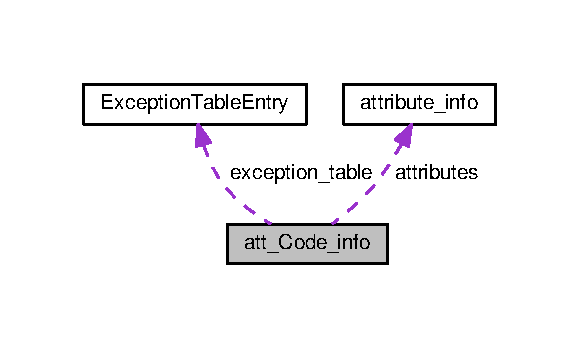
\includegraphics[width=278pt]{structatt__Code__info__coll__graph}
\end{center}
\end{figure}
\subsection*{Campos de Dados}
\begin{DoxyCompactItemize}
\item 
uint16\+\_\+t \hyperlink{structatt__Code__info_aa2d5de07b8832d1cd18a3e4779348fe3}{max\+\_\+stack}
\item 
uint16\+\_\+t \hyperlink{structatt__Code__info_acc9a5f7316ef5c5e051f88646bacf445}{max\+\_\+locals}
\item 
uint32\+\_\+t \hyperlink{structatt__Code__info_a24832826292dff47147e23f9d440bd2a}{code\+\_\+length}
\item 
uint8\+\_\+t $\ast$ \hyperlink{structatt__Code__info_a8fb8f2fa609ccf1786492efca32d3be9}{code}
\item 
uint16\+\_\+t \hyperlink{structatt__Code__info_aacd07775342d4f5ace7485e36e2e5e3b}{exception\+\_\+table\+\_\+length}
\item 
\hyperlink{structExceptionTableEntry}{Exception\+Table\+Entry} $\ast$ \hyperlink{structatt__Code__info_af5c5d84bb1f725dc949981cc752c45d2}{exception\+\_\+table}
\item 
uint16\+\_\+t \hyperlink{structatt__Code__info_a9bed6599acdfbf0b3391c827272a5502}{attributes\+\_\+count}
\item 
\hyperlink{structattribute__info}{attribute\+\_\+info} $\ast$ \hyperlink{structatt__Code__info_a09d52ef82f22bf27c4b5e3f2ab021f79}{attributes}
\end{DoxyCompactItemize}


\subsection{Documentação dos campos e atributos}
\index{att\+\_\+\+Code\+\_\+info@{att\+\_\+\+Code\+\_\+info}!attributes@{attributes}}
\index{attributes@{attributes}!att\+\_\+\+Code\+\_\+info@{att\+\_\+\+Code\+\_\+info}}
\subsubsection[{\texorpdfstring{attributes}{attributes}}]{\setlength{\rightskip}{0pt plus 5cm}{\bf attribute\+\_\+info}$\ast$ att\+\_\+\+Code\+\_\+info\+::attributes}\hypertarget{structatt__Code__info_a09d52ef82f22bf27c4b5e3f2ab021f79}{}\label{structatt__Code__info_a09d52ef82f22bf27c4b5e3f2ab021f79}
\index{att\+\_\+\+Code\+\_\+info@{att\+\_\+\+Code\+\_\+info}!attributes\+\_\+count@{attributes\+\_\+count}}
\index{attributes\+\_\+count@{attributes\+\_\+count}!att\+\_\+\+Code\+\_\+info@{att\+\_\+\+Code\+\_\+info}}
\subsubsection[{\texorpdfstring{attributes\+\_\+count}{attributes_count}}]{\setlength{\rightskip}{0pt plus 5cm}uint16\+\_\+t att\+\_\+\+Code\+\_\+info\+::attributes\+\_\+count}\hypertarget{structatt__Code__info_a9bed6599acdfbf0b3391c827272a5502}{}\label{structatt__Code__info_a9bed6599acdfbf0b3391c827272a5502}
\index{att\+\_\+\+Code\+\_\+info@{att\+\_\+\+Code\+\_\+info}!code@{code}}
\index{code@{code}!att\+\_\+\+Code\+\_\+info@{att\+\_\+\+Code\+\_\+info}}
\subsubsection[{\texorpdfstring{code}{code}}]{\setlength{\rightskip}{0pt plus 5cm}uint8\+\_\+t$\ast$ att\+\_\+\+Code\+\_\+info\+::code}\hypertarget{structatt__Code__info_a8fb8f2fa609ccf1786492efca32d3be9}{}\label{structatt__Code__info_a8fb8f2fa609ccf1786492efca32d3be9}
\index{att\+\_\+\+Code\+\_\+info@{att\+\_\+\+Code\+\_\+info}!code\+\_\+length@{code\+\_\+length}}
\index{code\+\_\+length@{code\+\_\+length}!att\+\_\+\+Code\+\_\+info@{att\+\_\+\+Code\+\_\+info}}
\subsubsection[{\texorpdfstring{code\+\_\+length}{code_length}}]{\setlength{\rightskip}{0pt plus 5cm}uint32\+\_\+t att\+\_\+\+Code\+\_\+info\+::code\+\_\+length}\hypertarget{structatt__Code__info_a24832826292dff47147e23f9d440bd2a}{}\label{structatt__Code__info_a24832826292dff47147e23f9d440bd2a}
\index{att\+\_\+\+Code\+\_\+info@{att\+\_\+\+Code\+\_\+info}!exception\+\_\+table@{exception\+\_\+table}}
\index{exception\+\_\+table@{exception\+\_\+table}!att\+\_\+\+Code\+\_\+info@{att\+\_\+\+Code\+\_\+info}}
\subsubsection[{\texorpdfstring{exception\+\_\+table}{exception_table}}]{\setlength{\rightskip}{0pt plus 5cm}{\bf Exception\+Table\+Entry}$\ast$ att\+\_\+\+Code\+\_\+info\+::exception\+\_\+table}\hypertarget{structatt__Code__info_af5c5d84bb1f725dc949981cc752c45d2}{}\label{structatt__Code__info_af5c5d84bb1f725dc949981cc752c45d2}
\index{att\+\_\+\+Code\+\_\+info@{att\+\_\+\+Code\+\_\+info}!exception\+\_\+table\+\_\+length@{exception\+\_\+table\+\_\+length}}
\index{exception\+\_\+table\+\_\+length@{exception\+\_\+table\+\_\+length}!att\+\_\+\+Code\+\_\+info@{att\+\_\+\+Code\+\_\+info}}
\subsubsection[{\texorpdfstring{exception\+\_\+table\+\_\+length}{exception_table_length}}]{\setlength{\rightskip}{0pt plus 5cm}uint16\+\_\+t att\+\_\+\+Code\+\_\+info\+::exception\+\_\+table\+\_\+length}\hypertarget{structatt__Code__info_aacd07775342d4f5ace7485e36e2e5e3b}{}\label{structatt__Code__info_aacd07775342d4f5ace7485e36e2e5e3b}
\index{att\+\_\+\+Code\+\_\+info@{att\+\_\+\+Code\+\_\+info}!max\+\_\+locals@{max\+\_\+locals}}
\index{max\+\_\+locals@{max\+\_\+locals}!att\+\_\+\+Code\+\_\+info@{att\+\_\+\+Code\+\_\+info}}
\subsubsection[{\texorpdfstring{max\+\_\+locals}{max_locals}}]{\setlength{\rightskip}{0pt plus 5cm}uint16\+\_\+t att\+\_\+\+Code\+\_\+info\+::max\+\_\+locals}\hypertarget{structatt__Code__info_acc9a5f7316ef5c5e051f88646bacf445}{}\label{structatt__Code__info_acc9a5f7316ef5c5e051f88646bacf445}
\index{att\+\_\+\+Code\+\_\+info@{att\+\_\+\+Code\+\_\+info}!max\+\_\+stack@{max\+\_\+stack}}
\index{max\+\_\+stack@{max\+\_\+stack}!att\+\_\+\+Code\+\_\+info@{att\+\_\+\+Code\+\_\+info}}
\subsubsection[{\texorpdfstring{max\+\_\+stack}{max_stack}}]{\setlength{\rightskip}{0pt plus 5cm}uint16\+\_\+t att\+\_\+\+Code\+\_\+info\+::max\+\_\+stack}\hypertarget{structatt__Code__info_aa2d5de07b8832d1cd18a3e4779348fe3}{}\label{structatt__Code__info_aa2d5de07b8832d1cd18a3e4779348fe3}


A documentação para esta estrutura foi gerada a partir do seguinte ficheiro\+:\begin{DoxyCompactItemize}
\item 
src/\hyperlink{attributes_8h}{attributes.\+h}\end{DoxyCompactItemize}

\hypertarget{structatt__ConstantValue__info}{}\section{Referência à estrutura att\+\_\+\+Constant\+Value\+\_\+info}
\label{structatt__ConstantValue__info}\index{att\+\_\+\+Constant\+Value\+\_\+info@{att\+\_\+\+Constant\+Value\+\_\+info}}


{\ttfamily \#include $<$attributes.\+h$>$}

\subsection*{Campos de Dados}
\begin{DoxyCompactItemize}
\item 
uint16\+\_\+t \hyperlink{structatt__ConstantValue__info_a6d9c6fc03274f8dc77c2ea8c53744dfa}{constantvalue\+\_\+index}
\end{DoxyCompactItemize}


\subsection{Documentação dos campos e atributos}
\index{att\+\_\+\+Constant\+Value\+\_\+info@{att\+\_\+\+Constant\+Value\+\_\+info}!constantvalue\+\_\+index@{constantvalue\+\_\+index}}
\index{constantvalue\+\_\+index@{constantvalue\+\_\+index}!att\+\_\+\+Constant\+Value\+\_\+info@{att\+\_\+\+Constant\+Value\+\_\+info}}
\subsubsection[{\texorpdfstring{constantvalue\+\_\+index}{constantvalue_index}}]{\setlength{\rightskip}{0pt plus 5cm}uint16\+\_\+t att\+\_\+\+Constant\+Value\+\_\+info\+::constantvalue\+\_\+index}\hypertarget{structatt__ConstantValue__info_a6d9c6fc03274f8dc77c2ea8c53744dfa}{}\label{structatt__ConstantValue__info_a6d9c6fc03274f8dc77c2ea8c53744dfa}


A documentação para esta estrutura foi gerada a partir do seguinte ficheiro\+:\begin{DoxyCompactItemize}
\item 
src/\hyperlink{attributes_8h}{attributes.\+h}\end{DoxyCompactItemize}

\hypertarget{structatt__Exceptions__info}{}\section{Referência à estrutura att\+\_\+\+Exceptions\+\_\+info}
\label{structatt__Exceptions__info}\index{att\+\_\+\+Exceptions\+\_\+info@{att\+\_\+\+Exceptions\+\_\+info}}


{\ttfamily \#include $<$attributes.\+h$>$}

\subsection*{Campos de Dados}
\begin{DoxyCompactItemize}
\item 
uint16\+\_\+t \hyperlink{structatt__Exceptions__info_aa118cef845f2ff9472572598b79ef635}{number\+\_\+of\+\_\+exceptions}
\item 
uint16\+\_\+t $\ast$ \hyperlink{structatt__Exceptions__info_ae713b303537b79289f22216ddbcbfd56}{exception\+\_\+index\+\_\+table}
\end{DoxyCompactItemize}


\subsection{Documentação dos campos e atributos}
\index{att\+\_\+\+Exceptions\+\_\+info@{att\+\_\+\+Exceptions\+\_\+info}!exception\+\_\+index\+\_\+table@{exception\+\_\+index\+\_\+table}}
\index{exception\+\_\+index\+\_\+table@{exception\+\_\+index\+\_\+table}!att\+\_\+\+Exceptions\+\_\+info@{att\+\_\+\+Exceptions\+\_\+info}}
\subsubsection[{\texorpdfstring{exception\+\_\+index\+\_\+table}{exception_index_table}}]{\setlength{\rightskip}{0pt plus 5cm}uint16\+\_\+t$\ast$ att\+\_\+\+Exceptions\+\_\+info\+::exception\+\_\+index\+\_\+table}\hypertarget{structatt__Exceptions__info_ae713b303537b79289f22216ddbcbfd56}{}\label{structatt__Exceptions__info_ae713b303537b79289f22216ddbcbfd56}
\index{att\+\_\+\+Exceptions\+\_\+info@{att\+\_\+\+Exceptions\+\_\+info}!number\+\_\+of\+\_\+exceptions@{number\+\_\+of\+\_\+exceptions}}
\index{number\+\_\+of\+\_\+exceptions@{number\+\_\+of\+\_\+exceptions}!att\+\_\+\+Exceptions\+\_\+info@{att\+\_\+\+Exceptions\+\_\+info}}
\subsubsection[{\texorpdfstring{number\+\_\+of\+\_\+exceptions}{number_of_exceptions}}]{\setlength{\rightskip}{0pt plus 5cm}uint16\+\_\+t att\+\_\+\+Exceptions\+\_\+info\+::number\+\_\+of\+\_\+exceptions}\hypertarget{structatt__Exceptions__info_aa118cef845f2ff9472572598b79ef635}{}\label{structatt__Exceptions__info_aa118cef845f2ff9472572598b79ef635}


A documentação para esta estrutura foi gerada a partir do seguinte ficheiro\+:\begin{DoxyCompactItemize}
\item 
src/\hyperlink{attributes_8h}{attributes.\+h}\end{DoxyCompactItemize}

\hypertarget{structatt__InnerClasses__info}{}\section{Referência à estrutura att\+\_\+\+Inner\+Classes\+\_\+info}
\label{structatt__InnerClasses__info}\index{att\+\_\+\+Inner\+Classes\+\_\+info@{att\+\_\+\+Inner\+Classes\+\_\+info}}


{\ttfamily \#include $<$attributes.\+h$>$}



Diagrama de colaboração para att\+\_\+\+Inner\+Classes\+\_\+info\+:\nopagebreak
\begin{figure}[H]
\begin{center}
\leavevmode
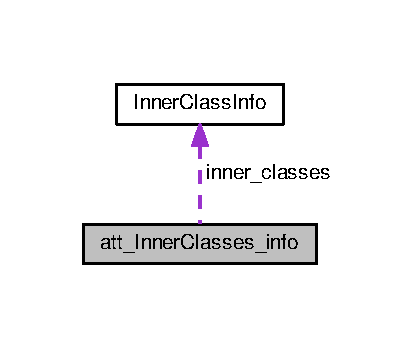
\includegraphics[width=200pt]{structatt__InnerClasses__info__coll__graph}
\end{center}
\end{figure}
\subsection*{Campos de Dados}
\begin{DoxyCompactItemize}
\item 
uint16\+\_\+t \hyperlink{structatt__InnerClasses__info_a8bb396e50023f850c80a70e0b736cc77}{number\+\_\+of\+\_\+classes}
\item 
\hyperlink{structInnerClassInfo}{Inner\+Class\+Info} $\ast$ \hyperlink{structatt__InnerClasses__info_a68beb2632952ef867172bfcfa327d256}{inner\+\_\+classes}
\end{DoxyCompactItemize}


\subsection{Documentação dos campos e atributos}
\index{att\+\_\+\+Inner\+Classes\+\_\+info@{att\+\_\+\+Inner\+Classes\+\_\+info}!inner\+\_\+classes@{inner\+\_\+classes}}
\index{inner\+\_\+classes@{inner\+\_\+classes}!att\+\_\+\+Inner\+Classes\+\_\+info@{att\+\_\+\+Inner\+Classes\+\_\+info}}
\subsubsection[{\texorpdfstring{inner\+\_\+classes}{inner_classes}}]{\setlength{\rightskip}{0pt plus 5cm}{\bf Inner\+Class\+Info}$\ast$ att\+\_\+\+Inner\+Classes\+\_\+info\+::inner\+\_\+classes}\hypertarget{structatt__InnerClasses__info_a68beb2632952ef867172bfcfa327d256}{}\label{structatt__InnerClasses__info_a68beb2632952ef867172bfcfa327d256}
\index{att\+\_\+\+Inner\+Classes\+\_\+info@{att\+\_\+\+Inner\+Classes\+\_\+info}!number\+\_\+of\+\_\+classes@{number\+\_\+of\+\_\+classes}}
\index{number\+\_\+of\+\_\+classes@{number\+\_\+of\+\_\+classes}!att\+\_\+\+Inner\+Classes\+\_\+info@{att\+\_\+\+Inner\+Classes\+\_\+info}}
\subsubsection[{\texorpdfstring{number\+\_\+of\+\_\+classes}{number_of_classes}}]{\setlength{\rightskip}{0pt plus 5cm}uint16\+\_\+t att\+\_\+\+Inner\+Classes\+\_\+info\+::number\+\_\+of\+\_\+classes}\hypertarget{structatt__InnerClasses__info_a8bb396e50023f850c80a70e0b736cc77}{}\label{structatt__InnerClasses__info_a8bb396e50023f850c80a70e0b736cc77}


A documentação para esta estrutura foi gerada a partir do seguinte ficheiro\+:\begin{DoxyCompactItemize}
\item 
src/\hyperlink{attributes_8h}{attributes.\+h}\end{DoxyCompactItemize}

\hypertarget{structatt__LineNumberTable__info}{}\section{Referência à estrutura att\+\_\+\+Line\+Number\+Table\+\_\+info}
\label{structatt__LineNumberTable__info}\index{att\+\_\+\+Line\+Number\+Table\+\_\+info@{att\+\_\+\+Line\+Number\+Table\+\_\+info}}


{\ttfamily \#include $<$attributes.\+h$>$}



Diagrama de colaboração para att\+\_\+\+Line\+Number\+Table\+\_\+info\+:\nopagebreak
\begin{figure}[H]
\begin{center}
\leavevmode
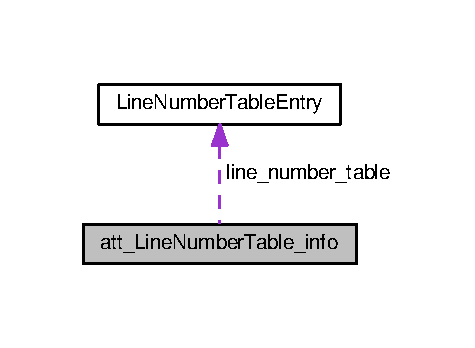
\includegraphics[width=228pt]{structatt__LineNumberTable__info__coll__graph}
\end{center}
\end{figure}
\subsection*{Campos de Dados}
\begin{DoxyCompactItemize}
\item 
uint16\+\_\+t \hyperlink{structatt__LineNumberTable__info_a6c335e2b6b14577d9a0e063cd5a361e0}{line\+\_\+number\+\_\+table\+\_\+length}
\item 
\hyperlink{structLineNumberTableEntry}{Line\+Number\+Table\+Entry} $\ast$ \hyperlink{structatt__LineNumberTable__info_ac9c52cc4b931ea8cfc746ea0a1d573ac}{line\+\_\+number\+\_\+table}
\end{DoxyCompactItemize}


\subsection{Documentação dos campos e atributos}
\index{att\+\_\+\+Line\+Number\+Table\+\_\+info@{att\+\_\+\+Line\+Number\+Table\+\_\+info}!line\+\_\+number\+\_\+table@{line\+\_\+number\+\_\+table}}
\index{line\+\_\+number\+\_\+table@{line\+\_\+number\+\_\+table}!att\+\_\+\+Line\+Number\+Table\+\_\+info@{att\+\_\+\+Line\+Number\+Table\+\_\+info}}
\subsubsection[{\texorpdfstring{line\+\_\+number\+\_\+table}{line_number_table}}]{\setlength{\rightskip}{0pt plus 5cm}{\bf Line\+Number\+Table\+Entry}$\ast$ att\+\_\+\+Line\+Number\+Table\+\_\+info\+::line\+\_\+number\+\_\+table}\hypertarget{structatt__LineNumberTable__info_ac9c52cc4b931ea8cfc746ea0a1d573ac}{}\label{structatt__LineNumberTable__info_ac9c52cc4b931ea8cfc746ea0a1d573ac}
\index{att\+\_\+\+Line\+Number\+Table\+\_\+info@{att\+\_\+\+Line\+Number\+Table\+\_\+info}!line\+\_\+number\+\_\+table\+\_\+length@{line\+\_\+number\+\_\+table\+\_\+length}}
\index{line\+\_\+number\+\_\+table\+\_\+length@{line\+\_\+number\+\_\+table\+\_\+length}!att\+\_\+\+Line\+Number\+Table\+\_\+info@{att\+\_\+\+Line\+Number\+Table\+\_\+info}}
\subsubsection[{\texorpdfstring{line\+\_\+number\+\_\+table\+\_\+length}{line_number_table_length}}]{\setlength{\rightskip}{0pt plus 5cm}uint16\+\_\+t att\+\_\+\+Line\+Number\+Table\+\_\+info\+::line\+\_\+number\+\_\+table\+\_\+length}\hypertarget{structatt__LineNumberTable__info_a6c335e2b6b14577d9a0e063cd5a361e0}{}\label{structatt__LineNumberTable__info_a6c335e2b6b14577d9a0e063cd5a361e0}


A documentação para esta estrutura foi gerada a partir do seguinte ficheiro\+:\begin{DoxyCompactItemize}
\item 
src/\hyperlink{attributes_8h}{attributes.\+h}\end{DoxyCompactItemize}

\hypertarget{structatt__SourceFile__info}{}\section{Referência à estrutura att\+\_\+\+Source\+File\+\_\+info}
\label{structatt__SourceFile__info}\index{att\+\_\+\+Source\+File\+\_\+info@{att\+\_\+\+Source\+File\+\_\+info}}


{\ttfamily \#include $<$attributes.\+h$>$}

\subsection*{Campos de Dados}
\begin{DoxyCompactItemize}
\item 
uint16\+\_\+t \hyperlink{structatt__SourceFile__info_a8cd88fda3147c1e7b1270dcc39754f1c}{sourcefile\+\_\+index}
\end{DoxyCompactItemize}


\subsection{Documentação dos campos e atributos}
\index{att\+\_\+\+Source\+File\+\_\+info@{att\+\_\+\+Source\+File\+\_\+info}!sourcefile\+\_\+index@{sourcefile\+\_\+index}}
\index{sourcefile\+\_\+index@{sourcefile\+\_\+index}!att\+\_\+\+Source\+File\+\_\+info@{att\+\_\+\+Source\+File\+\_\+info}}
\subsubsection[{\texorpdfstring{sourcefile\+\_\+index}{sourcefile_index}}]{\setlength{\rightskip}{0pt plus 5cm}uint16\+\_\+t att\+\_\+\+Source\+File\+\_\+info\+::sourcefile\+\_\+index}\hypertarget{structatt__SourceFile__info_a8cd88fda3147c1e7b1270dcc39754f1c}{}\label{structatt__SourceFile__info_a8cd88fda3147c1e7b1270dcc39754f1c}


A documentação para esta estrutura foi gerada a partir do seguinte ficheiro\+:\begin{DoxyCompactItemize}
\item 
src/\hyperlink{attributes_8h}{attributes.\+h}\end{DoxyCompactItemize}

\hypertarget{structattribute__info}{}\section{Referência à estrutura attribute\+\_\+info}
\label{structattribute__info}\index{attribute\+\_\+info@{attribute\+\_\+info}}


{\ttfamily \#include $<$attributes.\+h$>$}

\subsection*{Campos de Dados}
\begin{DoxyCompactItemize}
\item 
uint16\+\_\+t \hyperlink{structattribute__info_a7e925cf3d7a72731f1b6a6e4d1c24cc2}{name\+\_\+index}
\item 
uint32\+\_\+t \hyperlink{structattribute__info_a9528b298d46309f571f1f58c84cbd57c}{length}
\item 
void $\ast$ \hyperlink{structattribute__info_a7f168925308e418b7b44c9f11fdf42ae}{info}
\item 
uint8\+\_\+t \hyperlink{structattribute__info_aba7285ff2ef220420c41b51470921544}{attribute\+Type}
\end{DoxyCompactItemize}


\subsection{Documentação dos campos e atributos}
\index{attribute\+\_\+info@{attribute\+\_\+info}!attribute\+Type@{attribute\+Type}}
\index{attribute\+Type@{attribute\+Type}!attribute\+\_\+info@{attribute\+\_\+info}}
\subsubsection[{\texorpdfstring{attribute\+Type}{attributeType}}]{\setlength{\rightskip}{0pt plus 5cm}uint8\+\_\+t attribute\+\_\+info\+::attribute\+Type}\hypertarget{structattribute__info_aba7285ff2ef220420c41b51470921544}{}\label{structattribute__info_aba7285ff2ef220420c41b51470921544}
\index{attribute\+\_\+info@{attribute\+\_\+info}!info@{info}}
\index{info@{info}!attribute\+\_\+info@{attribute\+\_\+info}}
\subsubsection[{\texorpdfstring{info}{info}}]{\setlength{\rightskip}{0pt plus 5cm}void$\ast$ attribute\+\_\+info\+::info}\hypertarget{structattribute__info_a7f168925308e418b7b44c9f11fdf42ae}{}\label{structattribute__info_a7f168925308e418b7b44c9f11fdf42ae}
\index{attribute\+\_\+info@{attribute\+\_\+info}!length@{length}}
\index{length@{length}!attribute\+\_\+info@{attribute\+\_\+info}}
\subsubsection[{\texorpdfstring{length}{length}}]{\setlength{\rightskip}{0pt plus 5cm}uint32\+\_\+t attribute\+\_\+info\+::length}\hypertarget{structattribute__info_a9528b298d46309f571f1f58c84cbd57c}{}\label{structattribute__info_a9528b298d46309f571f1f58c84cbd57c}
\index{attribute\+\_\+info@{attribute\+\_\+info}!name\+\_\+index@{name\+\_\+index}}
\index{name\+\_\+index@{name\+\_\+index}!attribute\+\_\+info@{attribute\+\_\+info}}
\subsubsection[{\texorpdfstring{name\+\_\+index}{name_index}}]{\setlength{\rightskip}{0pt plus 5cm}uint16\+\_\+t attribute\+\_\+info\+::name\+\_\+index}\hypertarget{structattribute__info_a7e925cf3d7a72731f1b6a6e4d1c24cc2}{}\label{structattribute__info_a7e925cf3d7a72731f1b6a6e4d1c24cc2}


A documentação para esta estrutura foi gerada a partir do seguinte ficheiro\+:\begin{DoxyCompactItemize}
\item 
src/\hyperlink{attributes_8h}{attributes.\+h}\end{DoxyCompactItemize}

\hypertarget{structcp__info}{}\section{Referência à estrutura cp\+\_\+info}
\label{structcp__info}\index{cp\+\_\+info@{cp\+\_\+info}}


{\ttfamily \#include $<$constantpool.\+h$>$}

\subsection*{Campos de Dados}
\begin{DoxyCompactItemize}
\item 
uint8\+\_\+t \hyperlink{structcp__info_a29d87595bc993eb6cd53f30e8305ec74}{tag}
\item 
\begin{tabbing}
xx\=xx\=xx\=xx\=xx\=xx\=xx\=xx\=xx\=\kill
union \{\\
\>struct \{\\
\>\>uint16\_t \hyperlink{structcp__info_a3c8912fe67e7d3f9ce150aa6f5bec22d}{name\_index}\\
\>\} \hyperlink{structcp__info_aeb14fdcb3ba2363a18f2ecbeac15ac41}{Class}\\
\>struct \{\\
\>\>uint16\_t \hyperlink{structcp__info_aa63dfc7668d7eff682f88b09c48eddc8}{string\_index}\\
\>\} \hyperlink{structcp__info_a0e7c2a98e0cf4ffeb32047c7d78d835c}{String}\\
\>struct \{\\
\>\>uint16\_t \hyperlink{structcp__info_ab2b48e96f2178c47f9f6b683c9b2fc59}{class\_index}\\
\>\>uint16\_t \hyperlink{structcp__info_ad7a8733b3b078818a59cc33eb1fa7dc3}{name\_and\_type\_index}\\
\>\} \hyperlink{structcp__info_ac2cdad99f486a8e1bd1a66a06556a945}{Fieldref}\\
\>struct \{\\
\>\>uint16\_t \hyperlink{structcp__info_ab2b48e96f2178c47f9f6b683c9b2fc59}{class\_index}\\
\>\>uint16\_t \hyperlink{structcp__info_ad7a8733b3b078818a59cc33eb1fa7dc3}{name\_and\_type\_index}\\
\>\} \hyperlink{structcp__info_a3a2f2fccc08f122c44a2cd3405ee6264}{Methodref}\\
\>struct \{\\
\>\>uint16\_t \hyperlink{structcp__info_ab2b48e96f2178c47f9f6b683c9b2fc59}{class\_index}\\
\>\>uint16\_t \hyperlink{structcp__info_ad7a8733b3b078818a59cc33eb1fa7dc3}{name\_and\_type\_index}\\
\>\} \hyperlink{structcp__info_aa83f8676e24f088925c6502b78765d04}{InterfaceMethodref}\\
\>struct \{\\
\>\>uint16\_t \hyperlink{structcp__info_a3c8912fe67e7d3f9ce150aa6f5bec22d}{name\_index}\\
\>\>uint16\_t \hyperlink{structcp__info_aef3c90a1a874ca4acbc49029aaa0d4cb}{descriptor\_index}\\
\>\} \hyperlink{structcp__info_a992e807724524d5cdd537a646478e7c3}{NameAndType}\\
\>struct \{\\
\>\>uint32\_t \hyperlink{structcp__info_abdf544fc1b14cb7bfcb5ecabb74a0e84}{value}\\
\>\} \hyperlink{structcp__info_af859585c09920ad4589135731a78e772}{Integer}\\
\>struct \{\\
\>\>uint32\_t \hyperlink{structcp__info_a34ed0f597e452fbeb97cb0f551a678bb}{bytes}\\
\>\} \hyperlink{structcp__info_aa58271cb0f8e9d8827b2e99380f4b777}{Float}\\
\>struct \{\\
\>\>uint32\_t \hyperlink{structcp__info_a73d116220b0d9e7674ab0bd34bcb155a}{high}\\
\>\>uint32\_t \hyperlink{structcp__info_ae325e667e647b781e0691686049e50ec}{low}\\
\>\} \hyperlink{structcp__info_a000e2b8074c512960f81e10a1946ae94}{Long}\\
\>struct \{\\
\>\>uint32\_t \hyperlink{structcp__info_a73d116220b0d9e7674ab0bd34bcb155a}{high}\\
\>\>uint32\_t \hyperlink{structcp__info_ae325e667e647b781e0691686049e50ec}{low}\\
\>\} \hyperlink{structcp__info_aa42214f97b75a51fadba707aa3c29749}{Double}\\
\>struct \{\\
\>\>uint16\_t \hyperlink{structcp__info_afa18d3ff419ce300281ca759a20a2cc3}{length}\\
\>\>uint8\_t $\ast$ \hyperlink{structcp__info_a34c1da9248b884af89b5c91d55087100}{bytes}\\
\>\} \hyperlink{structcp__info_a25ee4592009bd74535de00796abf40eb}{Utf8}\\
\}; \\

\end{tabbing}\end{DoxyCompactItemize}


\subsection{Documentação dos campos e atributos}
\subsubsection[{\texorpdfstring{"@1}{@1}}]{\setlength{\rightskip}{0pt plus 5cm}union \{ ... \} }\hypertarget{structcp__info_ab2df10b8ac24e6e4dc2e383a68c00447}{}\label{structcp__info_ab2df10b8ac24e6e4dc2e383a68c00447}
\index{cp\+\_\+info@{cp\+\_\+info}!bytes@{bytes}}
\index{bytes@{bytes}!cp\+\_\+info@{cp\+\_\+info}}
\subsubsection[{\texorpdfstring{bytes}{bytes}}]{\setlength{\rightskip}{0pt plus 5cm}uint32\+\_\+t cp\+\_\+info\+::bytes}\hypertarget{structcp__info_a34ed0f597e452fbeb97cb0f551a678bb}{}\label{structcp__info_a34ed0f597e452fbeb97cb0f551a678bb}
\index{cp\+\_\+info@{cp\+\_\+info}!bytes@{bytes}}
\index{bytes@{bytes}!cp\+\_\+info@{cp\+\_\+info}}
\subsubsection[{\texorpdfstring{bytes}{bytes}}]{\setlength{\rightskip}{0pt plus 5cm}uint8\+\_\+t$\ast$ cp\+\_\+info\+::bytes}\hypertarget{structcp__info_a34c1da9248b884af89b5c91d55087100}{}\label{structcp__info_a34c1da9248b884af89b5c91d55087100}
\index{cp\+\_\+info@{cp\+\_\+info}!Class@{Class}}
\index{Class@{Class}!cp\+\_\+info@{cp\+\_\+info}}
\subsubsection[{\texorpdfstring{Class}{Class}}]{\setlength{\rightskip}{0pt plus 5cm}struct \{ ... \}   cp\+\_\+info\+::\+Class}\hypertarget{structcp__info_aeb14fdcb3ba2363a18f2ecbeac15ac41}{}\label{structcp__info_aeb14fdcb3ba2363a18f2ecbeac15ac41}
\index{cp\+\_\+info@{cp\+\_\+info}!class\+\_\+index@{class\+\_\+index}}
\index{class\+\_\+index@{class\+\_\+index}!cp\+\_\+info@{cp\+\_\+info}}
\subsubsection[{\texorpdfstring{class\+\_\+index}{class_index}}]{\setlength{\rightskip}{0pt plus 5cm}uint16\+\_\+t cp\+\_\+info\+::class\+\_\+index}\hypertarget{structcp__info_ab2b48e96f2178c47f9f6b683c9b2fc59}{}\label{structcp__info_ab2b48e96f2178c47f9f6b683c9b2fc59}
\index{cp\+\_\+info@{cp\+\_\+info}!descriptor\+\_\+index@{descriptor\+\_\+index}}
\index{descriptor\+\_\+index@{descriptor\+\_\+index}!cp\+\_\+info@{cp\+\_\+info}}
\subsubsection[{\texorpdfstring{descriptor\+\_\+index}{descriptor_index}}]{\setlength{\rightskip}{0pt plus 5cm}uint16\+\_\+t cp\+\_\+info\+::descriptor\+\_\+index}\hypertarget{structcp__info_aef3c90a1a874ca4acbc49029aaa0d4cb}{}\label{structcp__info_aef3c90a1a874ca4acbc49029aaa0d4cb}
\index{cp\+\_\+info@{cp\+\_\+info}!Double@{Double}}
\index{Double@{Double}!cp\+\_\+info@{cp\+\_\+info}}
\subsubsection[{\texorpdfstring{Double}{Double}}]{\setlength{\rightskip}{0pt plus 5cm}struct \{ ... \}   cp\+\_\+info\+::\+Double}\hypertarget{structcp__info_aa42214f97b75a51fadba707aa3c29749}{}\label{structcp__info_aa42214f97b75a51fadba707aa3c29749}
\index{cp\+\_\+info@{cp\+\_\+info}!Fieldref@{Fieldref}}
\index{Fieldref@{Fieldref}!cp\+\_\+info@{cp\+\_\+info}}
\subsubsection[{\texorpdfstring{Fieldref}{Fieldref}}]{\setlength{\rightskip}{0pt plus 5cm}struct \{ ... \}   cp\+\_\+info\+::\+Fieldref}\hypertarget{structcp__info_ac2cdad99f486a8e1bd1a66a06556a945}{}\label{structcp__info_ac2cdad99f486a8e1bd1a66a06556a945}
\index{cp\+\_\+info@{cp\+\_\+info}!Float@{Float}}
\index{Float@{Float}!cp\+\_\+info@{cp\+\_\+info}}
\subsubsection[{\texorpdfstring{Float}{Float}}]{\setlength{\rightskip}{0pt plus 5cm}struct \{ ... \}   cp\+\_\+info\+::\+Float}\hypertarget{structcp__info_aa58271cb0f8e9d8827b2e99380f4b777}{}\label{structcp__info_aa58271cb0f8e9d8827b2e99380f4b777}
\index{cp\+\_\+info@{cp\+\_\+info}!high@{high}}
\index{high@{high}!cp\+\_\+info@{cp\+\_\+info}}
\subsubsection[{\texorpdfstring{high}{high}}]{\setlength{\rightskip}{0pt plus 5cm}uint32\+\_\+t cp\+\_\+info\+::high}\hypertarget{structcp__info_a73d116220b0d9e7674ab0bd34bcb155a}{}\label{structcp__info_a73d116220b0d9e7674ab0bd34bcb155a}
\index{cp\+\_\+info@{cp\+\_\+info}!Integer@{Integer}}
\index{Integer@{Integer}!cp\+\_\+info@{cp\+\_\+info}}
\subsubsection[{\texorpdfstring{Integer}{Integer}}]{\setlength{\rightskip}{0pt plus 5cm}struct \{ ... \}   cp\+\_\+info\+::\+Integer}\hypertarget{structcp__info_af859585c09920ad4589135731a78e772}{}\label{structcp__info_af859585c09920ad4589135731a78e772}
\index{cp\+\_\+info@{cp\+\_\+info}!Interface\+Methodref@{Interface\+Methodref}}
\index{Interface\+Methodref@{Interface\+Methodref}!cp\+\_\+info@{cp\+\_\+info}}
\subsubsection[{\texorpdfstring{Interface\+Methodref}{InterfaceMethodref}}]{\setlength{\rightskip}{0pt plus 5cm}struct \{ ... \}   cp\+\_\+info\+::\+Interface\+Methodref}\hypertarget{structcp__info_aa83f8676e24f088925c6502b78765d04}{}\label{structcp__info_aa83f8676e24f088925c6502b78765d04}
\index{cp\+\_\+info@{cp\+\_\+info}!length@{length}}
\index{length@{length}!cp\+\_\+info@{cp\+\_\+info}}
\subsubsection[{\texorpdfstring{length}{length}}]{\setlength{\rightskip}{0pt plus 5cm}uint16\+\_\+t cp\+\_\+info\+::length}\hypertarget{structcp__info_afa18d3ff419ce300281ca759a20a2cc3}{}\label{structcp__info_afa18d3ff419ce300281ca759a20a2cc3}
\index{cp\+\_\+info@{cp\+\_\+info}!Long@{Long}}
\index{Long@{Long}!cp\+\_\+info@{cp\+\_\+info}}
\subsubsection[{\texorpdfstring{Long}{Long}}]{\setlength{\rightskip}{0pt plus 5cm}struct \{ ... \}   cp\+\_\+info\+::\+Long}\hypertarget{structcp__info_a000e2b8074c512960f81e10a1946ae94}{}\label{structcp__info_a000e2b8074c512960f81e10a1946ae94}
\index{cp\+\_\+info@{cp\+\_\+info}!low@{low}}
\index{low@{low}!cp\+\_\+info@{cp\+\_\+info}}
\subsubsection[{\texorpdfstring{low}{low}}]{\setlength{\rightskip}{0pt plus 5cm}uint32\+\_\+t cp\+\_\+info\+::low}\hypertarget{structcp__info_ae325e667e647b781e0691686049e50ec}{}\label{structcp__info_ae325e667e647b781e0691686049e50ec}
\index{cp\+\_\+info@{cp\+\_\+info}!Methodref@{Methodref}}
\index{Methodref@{Methodref}!cp\+\_\+info@{cp\+\_\+info}}
\subsubsection[{\texorpdfstring{Methodref}{Methodref}}]{\setlength{\rightskip}{0pt plus 5cm}struct \{ ... \}   cp\+\_\+info\+::\+Methodref}\hypertarget{structcp__info_a3a2f2fccc08f122c44a2cd3405ee6264}{}\label{structcp__info_a3a2f2fccc08f122c44a2cd3405ee6264}
\index{cp\+\_\+info@{cp\+\_\+info}!name\+\_\+and\+\_\+type\+\_\+index@{name\+\_\+and\+\_\+type\+\_\+index}}
\index{name\+\_\+and\+\_\+type\+\_\+index@{name\+\_\+and\+\_\+type\+\_\+index}!cp\+\_\+info@{cp\+\_\+info}}
\subsubsection[{\texorpdfstring{name\+\_\+and\+\_\+type\+\_\+index}{name_and_type_index}}]{\setlength{\rightskip}{0pt plus 5cm}uint16\+\_\+t cp\+\_\+info\+::name\+\_\+and\+\_\+type\+\_\+index}\hypertarget{structcp__info_ad7a8733b3b078818a59cc33eb1fa7dc3}{}\label{structcp__info_ad7a8733b3b078818a59cc33eb1fa7dc3}
\index{cp\+\_\+info@{cp\+\_\+info}!name\+\_\+index@{name\+\_\+index}}
\index{name\+\_\+index@{name\+\_\+index}!cp\+\_\+info@{cp\+\_\+info}}
\subsubsection[{\texorpdfstring{name\+\_\+index}{name_index}}]{\setlength{\rightskip}{0pt plus 5cm}uint16\+\_\+t cp\+\_\+info\+::name\+\_\+index}\hypertarget{structcp__info_a3c8912fe67e7d3f9ce150aa6f5bec22d}{}\label{structcp__info_a3c8912fe67e7d3f9ce150aa6f5bec22d}
\index{cp\+\_\+info@{cp\+\_\+info}!Name\+And\+Type@{Name\+And\+Type}}
\index{Name\+And\+Type@{Name\+And\+Type}!cp\+\_\+info@{cp\+\_\+info}}
\subsubsection[{\texorpdfstring{Name\+And\+Type}{NameAndType}}]{\setlength{\rightskip}{0pt plus 5cm}struct \{ ... \}   cp\+\_\+info\+::\+Name\+And\+Type}\hypertarget{structcp__info_a992e807724524d5cdd537a646478e7c3}{}\label{structcp__info_a992e807724524d5cdd537a646478e7c3}
\index{cp\+\_\+info@{cp\+\_\+info}!String@{String}}
\index{String@{String}!cp\+\_\+info@{cp\+\_\+info}}
\subsubsection[{\texorpdfstring{String}{String}}]{\setlength{\rightskip}{0pt plus 5cm}struct \{ ... \}   cp\+\_\+info\+::\+String}\hypertarget{structcp__info_a0e7c2a98e0cf4ffeb32047c7d78d835c}{}\label{structcp__info_a0e7c2a98e0cf4ffeb32047c7d78d835c}
\index{cp\+\_\+info@{cp\+\_\+info}!string\+\_\+index@{string\+\_\+index}}
\index{string\+\_\+index@{string\+\_\+index}!cp\+\_\+info@{cp\+\_\+info}}
\subsubsection[{\texorpdfstring{string\+\_\+index}{string_index}}]{\setlength{\rightskip}{0pt plus 5cm}uint16\+\_\+t cp\+\_\+info\+::string\+\_\+index}\hypertarget{structcp__info_aa63dfc7668d7eff682f88b09c48eddc8}{}\label{structcp__info_aa63dfc7668d7eff682f88b09c48eddc8}
\index{cp\+\_\+info@{cp\+\_\+info}!tag@{tag}}
\index{tag@{tag}!cp\+\_\+info@{cp\+\_\+info}}
\subsubsection[{\texorpdfstring{tag}{tag}}]{\setlength{\rightskip}{0pt plus 5cm}uint8\+\_\+t cp\+\_\+info\+::tag}\hypertarget{structcp__info_a29d87595bc993eb6cd53f30e8305ec74}{}\label{structcp__info_a29d87595bc993eb6cd53f30e8305ec74}
\index{cp\+\_\+info@{cp\+\_\+info}!Utf8@{Utf8}}
\index{Utf8@{Utf8}!cp\+\_\+info@{cp\+\_\+info}}
\subsubsection[{\texorpdfstring{Utf8}{Utf8}}]{\setlength{\rightskip}{0pt plus 5cm}struct \{ ... \}   cp\+\_\+info\+::\+Utf8}\hypertarget{structcp__info_a25ee4592009bd74535de00796abf40eb}{}\label{structcp__info_a25ee4592009bd74535de00796abf40eb}
\index{cp\+\_\+info@{cp\+\_\+info}!value@{value}}
\index{value@{value}!cp\+\_\+info@{cp\+\_\+info}}
\subsubsection[{\texorpdfstring{value}{value}}]{\setlength{\rightskip}{0pt plus 5cm}uint32\+\_\+t cp\+\_\+info\+::value}\hypertarget{structcp__info_abdf544fc1b14cb7bfcb5ecabb74a0e84}{}\label{structcp__info_abdf544fc1b14cb7bfcb5ecabb74a0e84}


A documentação para esta estrutura foi gerada a partir do seguinte ficheiro\+:\begin{DoxyCompactItemize}
\item 
src/\hyperlink{constantpool_8h}{constantpool.\+h}\end{DoxyCompactItemize}

\hypertarget{structExceptionTableEntry}{}\section{Referência à estrutura Exception\+Table\+Entry}
\label{structExceptionTableEntry}\index{Exception\+Table\+Entry@{Exception\+Table\+Entry}}


{\ttfamily \#include $<$attributes.\+h$>$}

\subsection*{Campos de Dados}
\begin{DoxyCompactItemize}
\item 
uint16\+\_\+t \hyperlink{structExceptionTableEntry_a2b590ee5474b087686f851f10e3f8f06}{start\+\_\+pc}
\item 
uint16\+\_\+t \hyperlink{structExceptionTableEntry_a876e2f736b1b5f4f081ce96b2923f23e}{end\+\_\+pc}
\item 
uint16\+\_\+t \hyperlink{structExceptionTableEntry_a3fd0ed5cca1781e941594ef0af475add}{handler\+\_\+pc}
\item 
uint16\+\_\+t \hyperlink{structExceptionTableEntry_a7c5ab5cc44557c2e4b92c4643683205d}{catch\+\_\+type}
\end{DoxyCompactItemize}


\subsection{Documentação dos campos e atributos}
\index{Exception\+Table\+Entry@{Exception\+Table\+Entry}!catch\+\_\+type@{catch\+\_\+type}}
\index{catch\+\_\+type@{catch\+\_\+type}!Exception\+Table\+Entry@{Exception\+Table\+Entry}}
\subsubsection[{\texorpdfstring{catch\+\_\+type}{catch_type}}]{\setlength{\rightskip}{0pt plus 5cm}uint16\+\_\+t Exception\+Table\+Entry\+::catch\+\_\+type}\hypertarget{structExceptionTableEntry_a7c5ab5cc44557c2e4b92c4643683205d}{}\label{structExceptionTableEntry_a7c5ab5cc44557c2e4b92c4643683205d}
\index{Exception\+Table\+Entry@{Exception\+Table\+Entry}!end\+\_\+pc@{end\+\_\+pc}}
\index{end\+\_\+pc@{end\+\_\+pc}!Exception\+Table\+Entry@{Exception\+Table\+Entry}}
\subsubsection[{\texorpdfstring{end\+\_\+pc}{end_pc}}]{\setlength{\rightskip}{0pt plus 5cm}uint16\+\_\+t Exception\+Table\+Entry\+::end\+\_\+pc}\hypertarget{structExceptionTableEntry_a876e2f736b1b5f4f081ce96b2923f23e}{}\label{structExceptionTableEntry_a876e2f736b1b5f4f081ce96b2923f23e}
\index{Exception\+Table\+Entry@{Exception\+Table\+Entry}!handler\+\_\+pc@{handler\+\_\+pc}}
\index{handler\+\_\+pc@{handler\+\_\+pc}!Exception\+Table\+Entry@{Exception\+Table\+Entry}}
\subsubsection[{\texorpdfstring{handler\+\_\+pc}{handler_pc}}]{\setlength{\rightskip}{0pt plus 5cm}uint16\+\_\+t Exception\+Table\+Entry\+::handler\+\_\+pc}\hypertarget{structExceptionTableEntry_a3fd0ed5cca1781e941594ef0af475add}{}\label{structExceptionTableEntry_a3fd0ed5cca1781e941594ef0af475add}
\index{Exception\+Table\+Entry@{Exception\+Table\+Entry}!start\+\_\+pc@{start\+\_\+pc}}
\index{start\+\_\+pc@{start\+\_\+pc}!Exception\+Table\+Entry@{Exception\+Table\+Entry}}
\subsubsection[{\texorpdfstring{start\+\_\+pc}{start_pc}}]{\setlength{\rightskip}{0pt plus 5cm}uint16\+\_\+t Exception\+Table\+Entry\+::start\+\_\+pc}\hypertarget{structExceptionTableEntry_a2b590ee5474b087686f851f10e3f8f06}{}\label{structExceptionTableEntry_a2b590ee5474b087686f851f10e3f8f06}


A documentação para esta estrutura foi gerada a partir do seguinte ficheiro\+:\begin{DoxyCompactItemize}
\item 
src/\hyperlink{attributes_8h}{attributes.\+h}\end{DoxyCompactItemize}

\hypertarget{structfield__info}{}\section{Referência à estrutura field\+\_\+info}
\label{structfield__info}\index{field\+\_\+info@{field\+\_\+info}}


{\ttfamily \#include $<$fields.\+h$>$}



Diagrama de colaboração para field\+\_\+info\+:\nopagebreak
\begin{figure}[H]
\begin{center}
\leavevmode
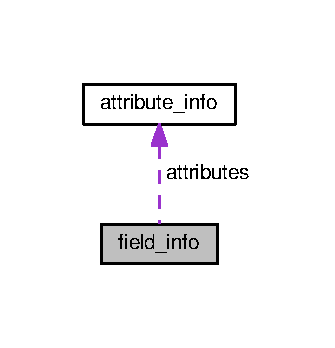
\includegraphics[width=161pt]{structfield__info__coll__graph}
\end{center}
\end{figure}
\subsection*{Campos de Dados}
\begin{DoxyCompactItemize}
\item 
uint16\+\_\+t \hyperlink{structfield__info_a97bcc8f6647cee71ea02bdd4183ba1da}{access\+\_\+flags}
\item 
uint16\+\_\+t \hyperlink{structfield__info_a3041f6a85347269c5253f7d377384b06}{name\+\_\+index}
\item 
uint16\+\_\+t \hyperlink{structfield__info_a56345eae0135047540b60ca34c91eb46}{descriptor\+\_\+index}
\item 
uint16\+\_\+t \hyperlink{structfield__info_a26aebef0abc97afef9e9a34701e6b550}{attributes\+\_\+count}
\item 
\hyperlink{structattribute__info}{attribute\+\_\+info} $\ast$ \hyperlink{structfield__info_afdda114944ae5eaae78c237f99257108}{attributes}
\end{DoxyCompactItemize}


\subsection{Documentação dos campos e atributos}
\index{field\+\_\+info@{field\+\_\+info}!access\+\_\+flags@{access\+\_\+flags}}
\index{access\+\_\+flags@{access\+\_\+flags}!field\+\_\+info@{field\+\_\+info}}
\subsubsection[{\texorpdfstring{access\+\_\+flags}{access_flags}}]{\setlength{\rightskip}{0pt plus 5cm}uint16\+\_\+t field\+\_\+info\+::access\+\_\+flags}\hypertarget{structfield__info_a97bcc8f6647cee71ea02bdd4183ba1da}{}\label{structfield__info_a97bcc8f6647cee71ea02bdd4183ba1da}
\index{field\+\_\+info@{field\+\_\+info}!attributes@{attributes}}
\index{attributes@{attributes}!field\+\_\+info@{field\+\_\+info}}
\subsubsection[{\texorpdfstring{attributes}{attributes}}]{\setlength{\rightskip}{0pt plus 5cm}{\bf attribute\+\_\+info}$\ast$ field\+\_\+info\+::attributes}\hypertarget{structfield__info_afdda114944ae5eaae78c237f99257108}{}\label{structfield__info_afdda114944ae5eaae78c237f99257108}
\index{field\+\_\+info@{field\+\_\+info}!attributes\+\_\+count@{attributes\+\_\+count}}
\index{attributes\+\_\+count@{attributes\+\_\+count}!field\+\_\+info@{field\+\_\+info}}
\subsubsection[{\texorpdfstring{attributes\+\_\+count}{attributes_count}}]{\setlength{\rightskip}{0pt plus 5cm}uint16\+\_\+t field\+\_\+info\+::attributes\+\_\+count}\hypertarget{structfield__info_a26aebef0abc97afef9e9a34701e6b550}{}\label{structfield__info_a26aebef0abc97afef9e9a34701e6b550}
\index{field\+\_\+info@{field\+\_\+info}!descriptor\+\_\+index@{descriptor\+\_\+index}}
\index{descriptor\+\_\+index@{descriptor\+\_\+index}!field\+\_\+info@{field\+\_\+info}}
\subsubsection[{\texorpdfstring{descriptor\+\_\+index}{descriptor_index}}]{\setlength{\rightskip}{0pt plus 5cm}uint16\+\_\+t field\+\_\+info\+::descriptor\+\_\+index}\hypertarget{structfield__info_a56345eae0135047540b60ca34c91eb46}{}\label{structfield__info_a56345eae0135047540b60ca34c91eb46}
\index{field\+\_\+info@{field\+\_\+info}!name\+\_\+index@{name\+\_\+index}}
\index{name\+\_\+index@{name\+\_\+index}!field\+\_\+info@{field\+\_\+info}}
\subsubsection[{\texorpdfstring{name\+\_\+index}{name_index}}]{\setlength{\rightskip}{0pt plus 5cm}uint16\+\_\+t field\+\_\+info\+::name\+\_\+index}\hypertarget{structfield__info_a3041f6a85347269c5253f7d377384b06}{}\label{structfield__info_a3041f6a85347269c5253f7d377384b06}


A documentação para esta estrutura foi gerada a partir do seguinte ficheiro\+:\begin{DoxyCompactItemize}
\item 
src/\hyperlink{fields_8h}{fields.\+h}\end{DoxyCompactItemize}

\hypertarget{structFrame}{}\section{Referência à estrutura Frame}
\label{structFrame}\index{Frame@{Frame}}


{\ttfamily \#include $<$framestack.\+h$>$}



Diagrama de colaboração para Frame\+:\nopagebreak
\begin{figure}[H]
\begin{center}
\leavevmode
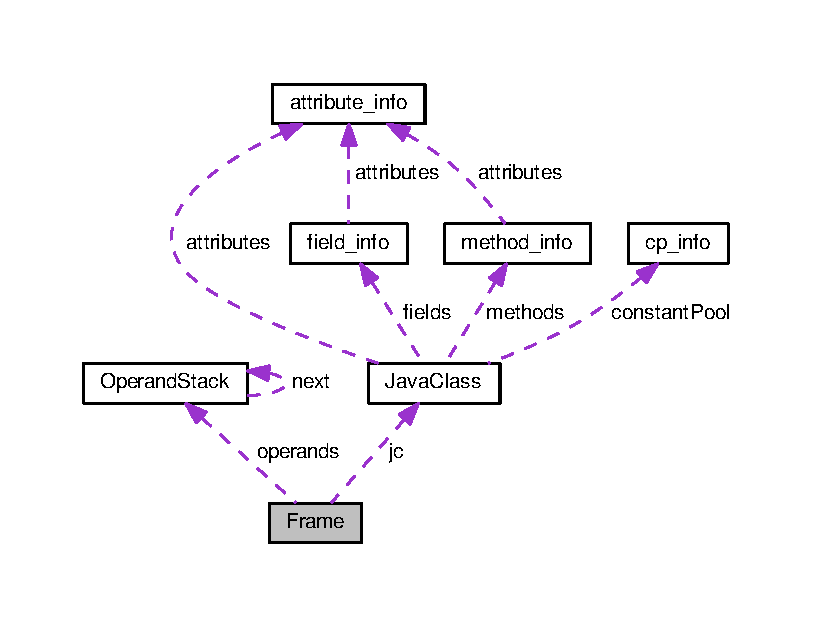
\includegraphics[width=350pt]{structFrame__coll__graph}
\end{center}
\end{figure}
\subsection*{Campos de Dados}
\begin{DoxyCompactItemize}
\item 
\hyperlink{structJavaClass}{Java\+Class} $\ast$ \hyperlink{structFrame_a6a053c391bc6b65491e72d2fc8ef360f}{jc}
\item 
uint32\+\_\+t \hyperlink{structFrame_a91e50d2091184efb52b6d7c0c21fd4b2}{pc}
\item 
uint32\+\_\+t \hyperlink{structFrame_a33a0dd3a739e1dcfd8b03621c752bb28}{code\+\_\+length}
\item 
uint8\+\_\+t $\ast$ \hyperlink{structFrame_a9de8be272246d00c7a0c2ddc899fe8f2}{code}
\item 
\hyperlink{structOperandStack}{Operand\+Stack} $\ast$ \hyperlink{structFrame_a0be587b8515083ff6d3c4e55918a7657}{operands}
\item 
int32\+\_\+t $\ast$ \hyperlink{structFrame_a9047c9524d44fc81cb6311de8a2a8b77}{local\+Variables}
\end{DoxyCompactItemize}


\subsection{Documentação dos campos e atributos}
\index{Frame@{Frame}!code@{code}}
\index{code@{code}!Frame@{Frame}}
\subsubsection[{\texorpdfstring{code}{code}}]{\setlength{\rightskip}{0pt plus 5cm}uint8\+\_\+t$\ast$ Frame\+::code}\hypertarget{structFrame_a9de8be272246d00c7a0c2ddc899fe8f2}{}\label{structFrame_a9de8be272246d00c7a0c2ddc899fe8f2}
\index{Frame@{Frame}!code\+\_\+length@{code\+\_\+length}}
\index{code\+\_\+length@{code\+\_\+length}!Frame@{Frame}}
\subsubsection[{\texorpdfstring{code\+\_\+length}{code_length}}]{\setlength{\rightskip}{0pt plus 5cm}uint32\+\_\+t Frame\+::code\+\_\+length}\hypertarget{structFrame_a33a0dd3a739e1dcfd8b03621c752bb28}{}\label{structFrame_a33a0dd3a739e1dcfd8b03621c752bb28}
\index{Frame@{Frame}!jc@{jc}}
\index{jc@{jc}!Frame@{Frame}}
\subsubsection[{\texorpdfstring{jc}{jc}}]{\setlength{\rightskip}{0pt plus 5cm}{\bf Java\+Class}$\ast$ Frame\+::jc}\hypertarget{structFrame_a6a053c391bc6b65491e72d2fc8ef360f}{}\label{structFrame_a6a053c391bc6b65491e72d2fc8ef360f}
\index{Frame@{Frame}!local\+Variables@{local\+Variables}}
\index{local\+Variables@{local\+Variables}!Frame@{Frame}}
\subsubsection[{\texorpdfstring{local\+Variables}{localVariables}}]{\setlength{\rightskip}{0pt plus 5cm}int32\+\_\+t$\ast$ Frame\+::local\+Variables}\hypertarget{structFrame_a9047c9524d44fc81cb6311de8a2a8b77}{}\label{structFrame_a9047c9524d44fc81cb6311de8a2a8b77}
\index{Frame@{Frame}!operands@{operands}}
\index{operands@{operands}!Frame@{Frame}}
\subsubsection[{\texorpdfstring{operands}{operands}}]{\setlength{\rightskip}{0pt plus 5cm}{\bf Operand\+Stack}$\ast$ Frame\+::operands}\hypertarget{structFrame_a0be587b8515083ff6d3c4e55918a7657}{}\label{structFrame_a0be587b8515083ff6d3c4e55918a7657}
\index{Frame@{Frame}!pc@{pc}}
\index{pc@{pc}!Frame@{Frame}}
\subsubsection[{\texorpdfstring{pc}{pc}}]{\setlength{\rightskip}{0pt plus 5cm}uint32\+\_\+t Frame\+::pc}\hypertarget{structFrame_a91e50d2091184efb52b6d7c0c21fd4b2}{}\label{structFrame_a91e50d2091184efb52b6d7c0c21fd4b2}


A documentação para esta estrutura foi gerada a partir do seguinte ficheiro\+:\begin{DoxyCompactItemize}
\item 
src/\hyperlink{framestack_8h}{framestack.\+h}\end{DoxyCompactItemize}

\hypertarget{structFrameStack}{}\section{Referência à estrutura Frame\+Stack}
\label{structFrameStack}\index{Frame\+Stack@{Frame\+Stack}}


{\ttfamily \#include $<$framestack.\+h$>$}



Diagrama de colaboração para Frame\+Stack\+:\nopagebreak
\begin{figure}[H]
\begin{center}
\leavevmode
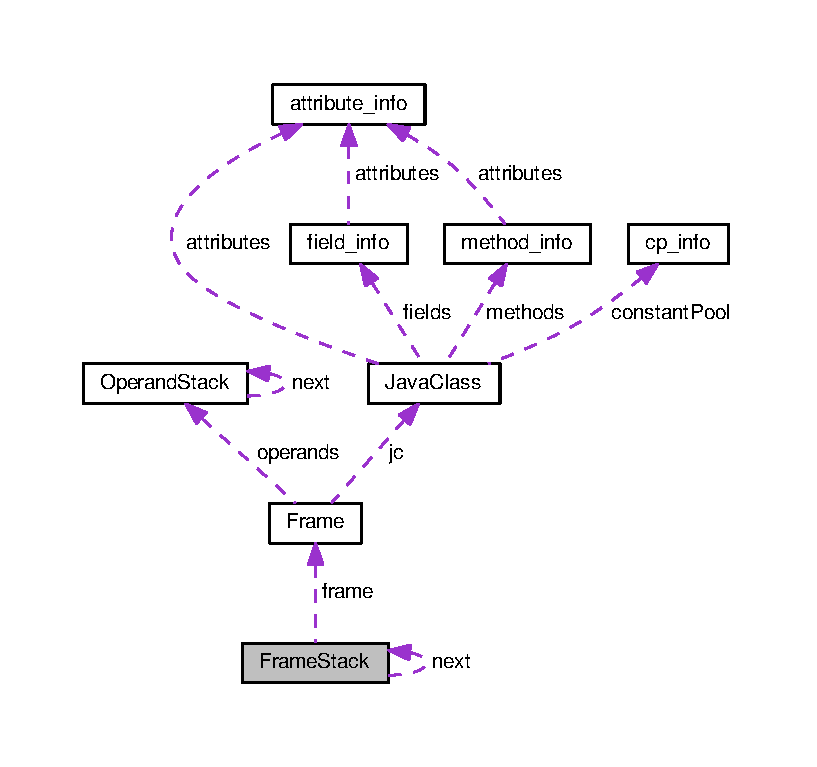
\includegraphics[width=350pt]{structFrameStack__coll__graph}
\end{center}
\end{figure}
\subsection*{Campos de Dados}
\begin{DoxyCompactItemize}
\item 
\hyperlink{structFrame}{Frame} $\ast$ \hyperlink{structFrameStack_a6175986505277602d1e3cdc9fbbfb8b4}{frame}
\item 
struct \hyperlink{structFrameStack}{Frame\+Stack} $\ast$ \hyperlink{structFrameStack_a7b333d40fd3fda54503169413dec8ddd}{next}
\end{DoxyCompactItemize}


\subsection{Documentação dos campos e atributos}
\index{Frame\+Stack@{Frame\+Stack}!frame@{frame}}
\index{frame@{frame}!Frame\+Stack@{Frame\+Stack}}
\subsubsection[{\texorpdfstring{frame}{frame}}]{\setlength{\rightskip}{0pt plus 5cm}{\bf Frame}$\ast$ Frame\+Stack\+::frame}\hypertarget{structFrameStack_a6175986505277602d1e3cdc9fbbfb8b4}{}\label{structFrameStack_a6175986505277602d1e3cdc9fbbfb8b4}
\index{Frame\+Stack@{Frame\+Stack}!next@{next}}
\index{next@{next}!Frame\+Stack@{Frame\+Stack}}
\subsubsection[{\texorpdfstring{next}{next}}]{\setlength{\rightskip}{0pt plus 5cm}struct {\bf Frame\+Stack}$\ast$ Frame\+Stack\+::next}\hypertarget{structFrameStack_a7b333d40fd3fda54503169413dec8ddd}{}\label{structFrameStack_a7b333d40fd3fda54503169413dec8ddd}


A documentação para esta estrutura foi gerada a partir do seguinte ficheiro\+:\begin{DoxyCompactItemize}
\item 
src/\hyperlink{framestack_8h}{framestack.\+h}\end{DoxyCompactItemize}

\hypertarget{structInnerClassInfo}{}\section{Referência à estrutura Inner\+Class\+Info}
\label{structInnerClassInfo}\index{Inner\+Class\+Info@{Inner\+Class\+Info}}


{\ttfamily \#include $<$attributes.\+h$>$}

\subsection*{Campos de Dados}
\begin{DoxyCompactItemize}
\item 
uint16\+\_\+t \hyperlink{structInnerClassInfo_a3383bc5bea2999b6bd91b9dfc095264f}{inner\+\_\+class\+\_\+index}
\item 
uint16\+\_\+t \hyperlink{structInnerClassInfo_a8449c27dc3cac6e437f4e1c1132ea229}{outer\+\_\+class\+\_\+index}
\item 
uint16\+\_\+t \hyperlink{structInnerClassInfo_a6d008047cb2df8aa856666169f625026}{inner\+\_\+class\+\_\+name\+\_\+index}
\item 
uint16\+\_\+t \hyperlink{structInnerClassInfo_a3810439736cc7ad5cdd1d2cb7aa7c885}{inner\+\_\+class\+\_\+access\+\_\+flags}
\end{DoxyCompactItemize}


\subsection{Documentação dos campos e atributos}
\index{Inner\+Class\+Info@{Inner\+Class\+Info}!inner\+\_\+class\+\_\+access\+\_\+flags@{inner\+\_\+class\+\_\+access\+\_\+flags}}
\index{inner\+\_\+class\+\_\+access\+\_\+flags@{inner\+\_\+class\+\_\+access\+\_\+flags}!Inner\+Class\+Info@{Inner\+Class\+Info}}
\subsubsection[{\texorpdfstring{inner\+\_\+class\+\_\+access\+\_\+flags}{inner_class_access_flags}}]{\setlength{\rightskip}{0pt plus 5cm}uint16\+\_\+t Inner\+Class\+Info\+::inner\+\_\+class\+\_\+access\+\_\+flags}\hypertarget{structInnerClassInfo_a3810439736cc7ad5cdd1d2cb7aa7c885}{}\label{structInnerClassInfo_a3810439736cc7ad5cdd1d2cb7aa7c885}
\index{Inner\+Class\+Info@{Inner\+Class\+Info}!inner\+\_\+class\+\_\+index@{inner\+\_\+class\+\_\+index}}
\index{inner\+\_\+class\+\_\+index@{inner\+\_\+class\+\_\+index}!Inner\+Class\+Info@{Inner\+Class\+Info}}
\subsubsection[{\texorpdfstring{inner\+\_\+class\+\_\+index}{inner_class_index}}]{\setlength{\rightskip}{0pt plus 5cm}uint16\+\_\+t Inner\+Class\+Info\+::inner\+\_\+class\+\_\+index}\hypertarget{structInnerClassInfo_a3383bc5bea2999b6bd91b9dfc095264f}{}\label{structInnerClassInfo_a3383bc5bea2999b6bd91b9dfc095264f}
\index{Inner\+Class\+Info@{Inner\+Class\+Info}!inner\+\_\+class\+\_\+name\+\_\+index@{inner\+\_\+class\+\_\+name\+\_\+index}}
\index{inner\+\_\+class\+\_\+name\+\_\+index@{inner\+\_\+class\+\_\+name\+\_\+index}!Inner\+Class\+Info@{Inner\+Class\+Info}}
\subsubsection[{\texorpdfstring{inner\+\_\+class\+\_\+name\+\_\+index}{inner_class_name_index}}]{\setlength{\rightskip}{0pt plus 5cm}uint16\+\_\+t Inner\+Class\+Info\+::inner\+\_\+class\+\_\+name\+\_\+index}\hypertarget{structInnerClassInfo_a6d008047cb2df8aa856666169f625026}{}\label{structInnerClassInfo_a6d008047cb2df8aa856666169f625026}
\index{Inner\+Class\+Info@{Inner\+Class\+Info}!outer\+\_\+class\+\_\+index@{outer\+\_\+class\+\_\+index}}
\index{outer\+\_\+class\+\_\+index@{outer\+\_\+class\+\_\+index}!Inner\+Class\+Info@{Inner\+Class\+Info}}
\subsubsection[{\texorpdfstring{outer\+\_\+class\+\_\+index}{outer_class_index}}]{\setlength{\rightskip}{0pt plus 5cm}uint16\+\_\+t Inner\+Class\+Info\+::outer\+\_\+class\+\_\+index}\hypertarget{structInnerClassInfo_a8449c27dc3cac6e437f4e1c1132ea229}{}\label{structInnerClassInfo_a8449c27dc3cac6e437f4e1c1132ea229}


A documentação para esta estrutura foi gerada a partir do seguinte ficheiro\+:\begin{DoxyCompactItemize}
\item 
src/\hyperlink{attributes_8h}{attributes.\+h}\end{DoxyCompactItemize}

\hypertarget{structJavaClass}{}\section{Referência à estrutura Java\+Class}
\label{structJavaClass}\index{Java\+Class@{Java\+Class}}


{\ttfamily \#include $<$javaclass.\+h$>$}



Diagrama de colaboração para Java\+Class\+:\nopagebreak
\begin{figure}[H]
\begin{center}
\leavevmode
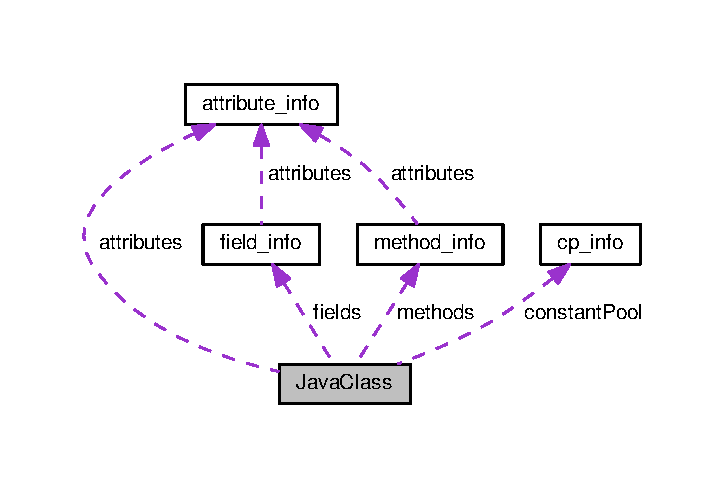
\includegraphics[width=349pt]{structJavaClass__coll__graph}
\end{center}
\end{figure}
\subsection*{Campos de Dados}
\begin{DoxyCompactItemize}
\item 
F\+I\+LE $\ast$ \hyperlink{structJavaClass_a24301fe0d812773595ca16c4ee658318}{file}
\item 
enum \hyperlink{javaclass_8h_a9b332e6330d199c30e246d4ad8bff5ac}{Java\+Class\+Status} \hyperlink{structJavaClass_aba868ba95744ed4200bd5bba1ad31ffc}{status}
\item 
uint16\+\_\+t \hyperlink{structJavaClass_a3961e984041068a78fa5b45414a94a00}{minor\+Version}
\item 
uint16\+\_\+t \hyperlink{structJavaClass_a7e6bc5cab0ffc5091e940cdb3b63e4eb}{major\+Version}
\item 
uint16\+\_\+t \hyperlink{structJavaClass_a89731a6218fb65b228ee1e056c368628}{constant\+Pool\+Count}
\item 
\hyperlink{structcp__info}{cp\+\_\+info} $\ast$ \hyperlink{structJavaClass_ad56dc000ce07c5c6ef57a1ef6f4859e0}{constant\+Pool}
\item 
uint16\+\_\+t \hyperlink{structJavaClass_a305af686b39aafe8248cb4b5af0f5ad4}{access\+Flags}
\item 
uint16\+\_\+t \hyperlink{structJavaClass_ac9af41263ddeabcfafd6464fd82c736f}{this\+Class}
\item 
uint16\+\_\+t \hyperlink{structJavaClass_a08240a259178c4576a82c688f4d3f8a8}{super\+Class}
\item 
uint16\+\_\+t \hyperlink{structJavaClass_a0abfb912729bc17c129e5460ae02dcd3}{interface\+Count}
\item 
uint16\+\_\+t $\ast$ \hyperlink{structJavaClass_a582289dae1229db46bbb8d733edf6a0a}{interfaces}
\item 
uint16\+\_\+t \hyperlink{structJavaClass_ac1568f2faaa136f0877d8a2962c00626}{field\+Count}
\item 
\hyperlink{structfield__info}{field\+\_\+info} $\ast$ \hyperlink{structJavaClass_a84f183bb9d29d499a5e910b9041acd14}{fields}
\item 
uint16\+\_\+t \hyperlink{structJavaClass_a4451678a1ac1921ddb929aced262d1d9}{method\+Count}
\item 
\hyperlink{structmethod__info}{method\+\_\+info} $\ast$ \hyperlink{structJavaClass_ab923c8f31c71ce1602ca21576a48bcb8}{methods}
\item 
uint16\+\_\+t \hyperlink{structJavaClass_ad04e4bd9744078e4f1f739f51295480e}{attribute\+Count}
\item 
\hyperlink{structattribute__info}{attribute\+\_\+info} $\ast$ \hyperlink{structJavaClass_ae90496c9f9b340ef216b24359cb2ff63}{attributes}
\item 
uint32\+\_\+t \hyperlink{structJavaClass_a58b471dbb758d2a3c1bbd6e0e90fb6e2}{total\+Bytes\+Read}
\item 
uint8\+\_\+t \hyperlink{structJavaClass_a57b0443668351c7380e3d8cdb3e97d7d}{last\+Tag\+Read}
\item 
int32\+\_\+t \hyperlink{structJavaClass_adedfcc5044efcb1c0798a87d52d30360}{current\+Constant\+Pool\+Entry\+Index}
\item 
int32\+\_\+t \hyperlink{structJavaClass_a7e50281e01408da883645af7d983570c}{constant\+Pool\+Entries\+Read}
\item 
int32\+\_\+t \hyperlink{structJavaClass_a45a51f67c49e0c528c212a65051bc349}{current\+Interface\+Entry\+Index}
\item 
int32\+\_\+t \hyperlink{structJavaClass_ad62c5545a3b4151e71bdc7b742606c55}{current\+Field\+Entry\+Index}
\item 
int32\+\_\+t \hyperlink{structJavaClass_a2a78abe9f88e0538b2912e6c72c22426}{current\+Method\+Entry\+Index}
\item 
int32\+\_\+t \hyperlink{structJavaClass_a26d4612d384289588b48be393c9705ac}{current\+Attribute\+Entry\+Index}
\item 
int32\+\_\+t \hyperlink{structJavaClass_aefcb0a0fbf6d98692680922792d74401}{attribute\+Entries\+Read}
\item 
int32\+\_\+t \hyperlink{structJavaClass_a785953f9978e474e59dada8ed5b17b25}{current\+Validity\+Entry\+Index}
\end{DoxyCompactItemize}


\subsection{Documentação dos campos e atributos}
\index{Java\+Class@{Java\+Class}!access\+Flags@{access\+Flags}}
\index{access\+Flags@{access\+Flags}!Java\+Class@{Java\+Class}}
\subsubsection[{\texorpdfstring{access\+Flags}{accessFlags}}]{\setlength{\rightskip}{0pt plus 5cm}uint16\+\_\+t Java\+Class\+::access\+Flags}\hypertarget{structJavaClass_a305af686b39aafe8248cb4b5af0f5ad4}{}\label{structJavaClass_a305af686b39aafe8248cb4b5af0f5ad4}
\index{Java\+Class@{Java\+Class}!attribute\+Count@{attribute\+Count}}
\index{attribute\+Count@{attribute\+Count}!Java\+Class@{Java\+Class}}
\subsubsection[{\texorpdfstring{attribute\+Count}{attributeCount}}]{\setlength{\rightskip}{0pt plus 5cm}uint16\+\_\+t Java\+Class\+::attribute\+Count}\hypertarget{structJavaClass_ad04e4bd9744078e4f1f739f51295480e}{}\label{structJavaClass_ad04e4bd9744078e4f1f739f51295480e}
\index{Java\+Class@{Java\+Class}!attribute\+Entries\+Read@{attribute\+Entries\+Read}}
\index{attribute\+Entries\+Read@{attribute\+Entries\+Read}!Java\+Class@{Java\+Class}}
\subsubsection[{\texorpdfstring{attribute\+Entries\+Read}{attributeEntriesRead}}]{\setlength{\rightskip}{0pt plus 5cm}int32\+\_\+t Java\+Class\+::attribute\+Entries\+Read}\hypertarget{structJavaClass_aefcb0a0fbf6d98692680922792d74401}{}\label{structJavaClass_aefcb0a0fbf6d98692680922792d74401}
\index{Java\+Class@{Java\+Class}!attributes@{attributes}}
\index{attributes@{attributes}!Java\+Class@{Java\+Class}}
\subsubsection[{\texorpdfstring{attributes}{attributes}}]{\setlength{\rightskip}{0pt plus 5cm}{\bf attribute\+\_\+info}$\ast$ Java\+Class\+::attributes}\hypertarget{structJavaClass_ae90496c9f9b340ef216b24359cb2ff63}{}\label{structJavaClass_ae90496c9f9b340ef216b24359cb2ff63}
\index{Java\+Class@{Java\+Class}!constant\+Pool@{constant\+Pool}}
\index{constant\+Pool@{constant\+Pool}!Java\+Class@{Java\+Class}}
\subsubsection[{\texorpdfstring{constant\+Pool}{constantPool}}]{\setlength{\rightskip}{0pt plus 5cm}{\bf cp\+\_\+info}$\ast$ Java\+Class\+::constant\+Pool}\hypertarget{structJavaClass_ad56dc000ce07c5c6ef57a1ef6f4859e0}{}\label{structJavaClass_ad56dc000ce07c5c6ef57a1ef6f4859e0}
\index{Java\+Class@{Java\+Class}!constant\+Pool\+Count@{constant\+Pool\+Count}}
\index{constant\+Pool\+Count@{constant\+Pool\+Count}!Java\+Class@{Java\+Class}}
\subsubsection[{\texorpdfstring{constant\+Pool\+Count}{constantPoolCount}}]{\setlength{\rightskip}{0pt plus 5cm}uint16\+\_\+t Java\+Class\+::constant\+Pool\+Count}\hypertarget{structJavaClass_a89731a6218fb65b228ee1e056c368628}{}\label{structJavaClass_a89731a6218fb65b228ee1e056c368628}
\index{Java\+Class@{Java\+Class}!constant\+Pool\+Entries\+Read@{constant\+Pool\+Entries\+Read}}
\index{constant\+Pool\+Entries\+Read@{constant\+Pool\+Entries\+Read}!Java\+Class@{Java\+Class}}
\subsubsection[{\texorpdfstring{constant\+Pool\+Entries\+Read}{constantPoolEntriesRead}}]{\setlength{\rightskip}{0pt plus 5cm}int32\+\_\+t Java\+Class\+::constant\+Pool\+Entries\+Read}\hypertarget{structJavaClass_a7e50281e01408da883645af7d983570c}{}\label{structJavaClass_a7e50281e01408da883645af7d983570c}
\index{Java\+Class@{Java\+Class}!current\+Attribute\+Entry\+Index@{current\+Attribute\+Entry\+Index}}
\index{current\+Attribute\+Entry\+Index@{current\+Attribute\+Entry\+Index}!Java\+Class@{Java\+Class}}
\subsubsection[{\texorpdfstring{current\+Attribute\+Entry\+Index}{currentAttributeEntryIndex}}]{\setlength{\rightskip}{0pt plus 5cm}int32\+\_\+t Java\+Class\+::current\+Attribute\+Entry\+Index}\hypertarget{structJavaClass_a26d4612d384289588b48be393c9705ac}{}\label{structJavaClass_a26d4612d384289588b48be393c9705ac}
\index{Java\+Class@{Java\+Class}!current\+Constant\+Pool\+Entry\+Index@{current\+Constant\+Pool\+Entry\+Index}}
\index{current\+Constant\+Pool\+Entry\+Index@{current\+Constant\+Pool\+Entry\+Index}!Java\+Class@{Java\+Class}}
\subsubsection[{\texorpdfstring{current\+Constant\+Pool\+Entry\+Index}{currentConstantPoolEntryIndex}}]{\setlength{\rightskip}{0pt plus 5cm}int32\+\_\+t Java\+Class\+::current\+Constant\+Pool\+Entry\+Index}\hypertarget{structJavaClass_adedfcc5044efcb1c0798a87d52d30360}{}\label{structJavaClass_adedfcc5044efcb1c0798a87d52d30360}
\index{Java\+Class@{Java\+Class}!current\+Field\+Entry\+Index@{current\+Field\+Entry\+Index}}
\index{current\+Field\+Entry\+Index@{current\+Field\+Entry\+Index}!Java\+Class@{Java\+Class}}
\subsubsection[{\texorpdfstring{current\+Field\+Entry\+Index}{currentFieldEntryIndex}}]{\setlength{\rightskip}{0pt plus 5cm}int32\+\_\+t Java\+Class\+::current\+Field\+Entry\+Index}\hypertarget{structJavaClass_ad62c5545a3b4151e71bdc7b742606c55}{}\label{structJavaClass_ad62c5545a3b4151e71bdc7b742606c55}
\index{Java\+Class@{Java\+Class}!current\+Interface\+Entry\+Index@{current\+Interface\+Entry\+Index}}
\index{current\+Interface\+Entry\+Index@{current\+Interface\+Entry\+Index}!Java\+Class@{Java\+Class}}
\subsubsection[{\texorpdfstring{current\+Interface\+Entry\+Index}{currentInterfaceEntryIndex}}]{\setlength{\rightskip}{0pt plus 5cm}int32\+\_\+t Java\+Class\+::current\+Interface\+Entry\+Index}\hypertarget{structJavaClass_a45a51f67c49e0c528c212a65051bc349}{}\label{structJavaClass_a45a51f67c49e0c528c212a65051bc349}
\index{Java\+Class@{Java\+Class}!current\+Method\+Entry\+Index@{current\+Method\+Entry\+Index}}
\index{current\+Method\+Entry\+Index@{current\+Method\+Entry\+Index}!Java\+Class@{Java\+Class}}
\subsubsection[{\texorpdfstring{current\+Method\+Entry\+Index}{currentMethodEntryIndex}}]{\setlength{\rightskip}{0pt plus 5cm}int32\+\_\+t Java\+Class\+::current\+Method\+Entry\+Index}\hypertarget{structJavaClass_a2a78abe9f88e0538b2912e6c72c22426}{}\label{structJavaClass_a2a78abe9f88e0538b2912e6c72c22426}
\index{Java\+Class@{Java\+Class}!current\+Validity\+Entry\+Index@{current\+Validity\+Entry\+Index}}
\index{current\+Validity\+Entry\+Index@{current\+Validity\+Entry\+Index}!Java\+Class@{Java\+Class}}
\subsubsection[{\texorpdfstring{current\+Validity\+Entry\+Index}{currentValidityEntryIndex}}]{\setlength{\rightskip}{0pt plus 5cm}int32\+\_\+t Java\+Class\+::current\+Validity\+Entry\+Index}\hypertarget{structJavaClass_a785953f9978e474e59dada8ed5b17b25}{}\label{structJavaClass_a785953f9978e474e59dada8ed5b17b25}
\index{Java\+Class@{Java\+Class}!field\+Count@{field\+Count}}
\index{field\+Count@{field\+Count}!Java\+Class@{Java\+Class}}
\subsubsection[{\texorpdfstring{field\+Count}{fieldCount}}]{\setlength{\rightskip}{0pt plus 5cm}uint16\+\_\+t Java\+Class\+::field\+Count}\hypertarget{structJavaClass_ac1568f2faaa136f0877d8a2962c00626}{}\label{structJavaClass_ac1568f2faaa136f0877d8a2962c00626}
\index{Java\+Class@{Java\+Class}!fields@{fields}}
\index{fields@{fields}!Java\+Class@{Java\+Class}}
\subsubsection[{\texorpdfstring{fields}{fields}}]{\setlength{\rightskip}{0pt plus 5cm}{\bf field\+\_\+info}$\ast$ Java\+Class\+::fields}\hypertarget{structJavaClass_a84f183bb9d29d499a5e910b9041acd14}{}\label{structJavaClass_a84f183bb9d29d499a5e910b9041acd14}
\index{Java\+Class@{Java\+Class}!file@{file}}
\index{file@{file}!Java\+Class@{Java\+Class}}
\subsubsection[{\texorpdfstring{file}{file}}]{\setlength{\rightskip}{0pt plus 5cm}F\+I\+LE$\ast$ Java\+Class\+::file}\hypertarget{structJavaClass_a24301fe0d812773595ca16c4ee658318}{}\label{structJavaClass_a24301fe0d812773595ca16c4ee658318}
\index{Java\+Class@{Java\+Class}!interface\+Count@{interface\+Count}}
\index{interface\+Count@{interface\+Count}!Java\+Class@{Java\+Class}}
\subsubsection[{\texorpdfstring{interface\+Count}{interfaceCount}}]{\setlength{\rightskip}{0pt plus 5cm}uint16\+\_\+t Java\+Class\+::interface\+Count}\hypertarget{structJavaClass_a0abfb912729bc17c129e5460ae02dcd3}{}\label{structJavaClass_a0abfb912729bc17c129e5460ae02dcd3}
\index{Java\+Class@{Java\+Class}!interfaces@{interfaces}}
\index{interfaces@{interfaces}!Java\+Class@{Java\+Class}}
\subsubsection[{\texorpdfstring{interfaces}{interfaces}}]{\setlength{\rightskip}{0pt plus 5cm}uint16\+\_\+t$\ast$ Java\+Class\+::interfaces}\hypertarget{structJavaClass_a582289dae1229db46bbb8d733edf6a0a}{}\label{structJavaClass_a582289dae1229db46bbb8d733edf6a0a}
\index{Java\+Class@{Java\+Class}!last\+Tag\+Read@{last\+Tag\+Read}}
\index{last\+Tag\+Read@{last\+Tag\+Read}!Java\+Class@{Java\+Class}}
\subsubsection[{\texorpdfstring{last\+Tag\+Read}{lastTagRead}}]{\setlength{\rightskip}{0pt plus 5cm}uint8\+\_\+t Java\+Class\+::last\+Tag\+Read}\hypertarget{structJavaClass_a57b0443668351c7380e3d8cdb3e97d7d}{}\label{structJavaClass_a57b0443668351c7380e3d8cdb3e97d7d}
\index{Java\+Class@{Java\+Class}!major\+Version@{major\+Version}}
\index{major\+Version@{major\+Version}!Java\+Class@{Java\+Class}}
\subsubsection[{\texorpdfstring{major\+Version}{majorVersion}}]{\setlength{\rightskip}{0pt plus 5cm}uint16\+\_\+t Java\+Class\+::major\+Version}\hypertarget{structJavaClass_a7e6bc5cab0ffc5091e940cdb3b63e4eb}{}\label{structJavaClass_a7e6bc5cab0ffc5091e940cdb3b63e4eb}
\index{Java\+Class@{Java\+Class}!method\+Count@{method\+Count}}
\index{method\+Count@{method\+Count}!Java\+Class@{Java\+Class}}
\subsubsection[{\texorpdfstring{method\+Count}{methodCount}}]{\setlength{\rightskip}{0pt plus 5cm}uint16\+\_\+t Java\+Class\+::method\+Count}\hypertarget{structJavaClass_a4451678a1ac1921ddb929aced262d1d9}{}\label{structJavaClass_a4451678a1ac1921ddb929aced262d1d9}
\index{Java\+Class@{Java\+Class}!methods@{methods}}
\index{methods@{methods}!Java\+Class@{Java\+Class}}
\subsubsection[{\texorpdfstring{methods}{methods}}]{\setlength{\rightskip}{0pt plus 5cm}{\bf method\+\_\+info}$\ast$ Java\+Class\+::methods}\hypertarget{structJavaClass_ab923c8f31c71ce1602ca21576a48bcb8}{}\label{structJavaClass_ab923c8f31c71ce1602ca21576a48bcb8}
\index{Java\+Class@{Java\+Class}!minor\+Version@{minor\+Version}}
\index{minor\+Version@{minor\+Version}!Java\+Class@{Java\+Class}}
\subsubsection[{\texorpdfstring{minor\+Version}{minorVersion}}]{\setlength{\rightskip}{0pt plus 5cm}uint16\+\_\+t Java\+Class\+::minor\+Version}\hypertarget{structJavaClass_a3961e984041068a78fa5b45414a94a00}{}\label{structJavaClass_a3961e984041068a78fa5b45414a94a00}
\index{Java\+Class@{Java\+Class}!status@{status}}
\index{status@{status}!Java\+Class@{Java\+Class}}
\subsubsection[{\texorpdfstring{status}{status}}]{\setlength{\rightskip}{0pt plus 5cm}enum {\bf Java\+Class\+Status} Java\+Class\+::status}\hypertarget{structJavaClass_aba868ba95744ed4200bd5bba1ad31ffc}{}\label{structJavaClass_aba868ba95744ed4200bd5bba1ad31ffc}
\index{Java\+Class@{Java\+Class}!super\+Class@{super\+Class}}
\index{super\+Class@{super\+Class}!Java\+Class@{Java\+Class}}
\subsubsection[{\texorpdfstring{super\+Class}{superClass}}]{\setlength{\rightskip}{0pt plus 5cm}uint16\+\_\+t Java\+Class\+::super\+Class}\hypertarget{structJavaClass_a08240a259178c4576a82c688f4d3f8a8}{}\label{structJavaClass_a08240a259178c4576a82c688f4d3f8a8}
\index{Java\+Class@{Java\+Class}!this\+Class@{this\+Class}}
\index{this\+Class@{this\+Class}!Java\+Class@{Java\+Class}}
\subsubsection[{\texorpdfstring{this\+Class}{thisClass}}]{\setlength{\rightskip}{0pt plus 5cm}uint16\+\_\+t Java\+Class\+::this\+Class}\hypertarget{structJavaClass_ac9af41263ddeabcfafd6464fd82c736f}{}\label{structJavaClass_ac9af41263ddeabcfafd6464fd82c736f}
\index{Java\+Class@{Java\+Class}!total\+Bytes\+Read@{total\+Bytes\+Read}}
\index{total\+Bytes\+Read@{total\+Bytes\+Read}!Java\+Class@{Java\+Class}}
\subsubsection[{\texorpdfstring{total\+Bytes\+Read}{totalBytesRead}}]{\setlength{\rightskip}{0pt plus 5cm}uint32\+\_\+t Java\+Class\+::total\+Bytes\+Read}\hypertarget{structJavaClass_a58b471dbb758d2a3c1bbd6e0e90fb6e2}{}\label{structJavaClass_a58b471dbb758d2a3c1bbd6e0e90fb6e2}


A documentação para esta estrutura foi gerada a partir do seguinte ficheiro\+:\begin{DoxyCompactItemize}
\item 
src/\hyperlink{javaclass_8h}{javaclass.\+h}\end{DoxyCompactItemize}

\hypertarget{structJavaVirtualMachine}{}\section{Referência à estrutura Java\+Virtual\+Machine}
\label{structJavaVirtualMachine}\index{Java\+Virtual\+Machine@{Java\+Virtual\+Machine}}


{\ttfamily \#include $<$jvm.\+h$>$}



Diagrama de colaboração para Java\+Virtual\+Machine\+:\nopagebreak
\begin{figure}[H]
\begin{center}
\leavevmode
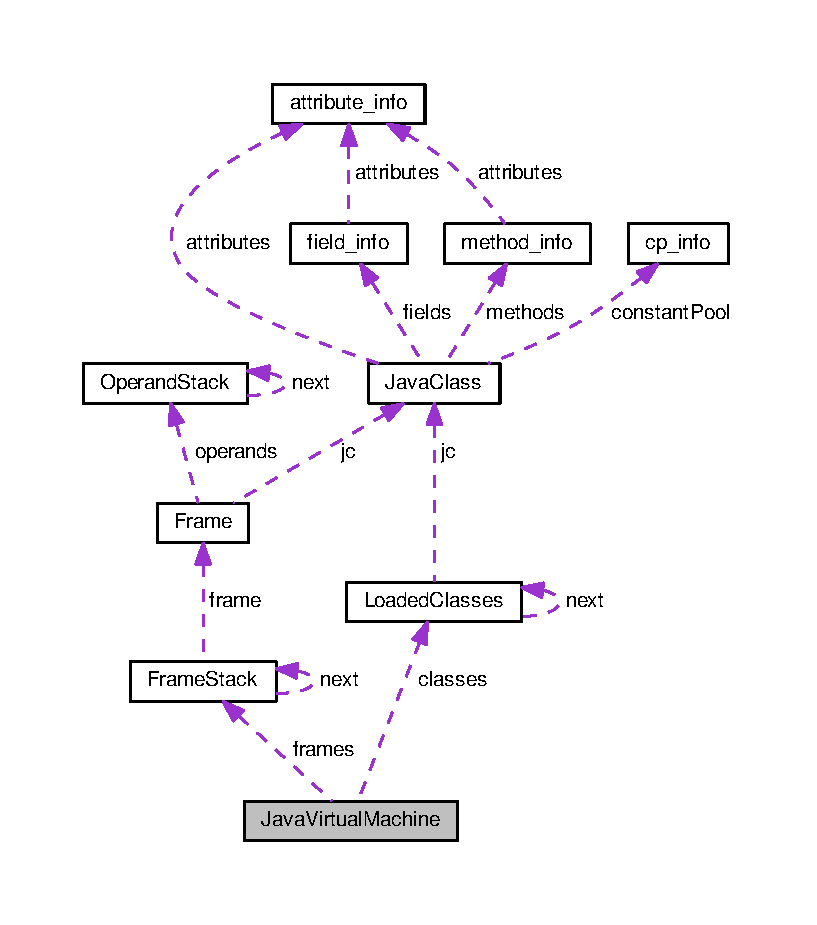
\includegraphics[width=350pt]{structJavaVirtualMachine__coll__graph}
\end{center}
\end{figure}
\subsection*{Campos de Dados}
\begin{DoxyCompactItemize}
\item 
uint8\+\_\+t \hyperlink{structJavaVirtualMachine_ae8571f20c0db273c88a5ce2d52d51a04}{status}
\item 
\hyperlink{structFrameStack}{Frame\+Stack} $\ast$ \hyperlink{structJavaVirtualMachine_a6a0d723bb649fabc57742221b01b3617}{frames}
\item 
\hyperlink{structLoadedClasses}{Loaded\+Classes} $\ast$ \hyperlink{structJavaVirtualMachine_a36266aec8ba9d25b4d9f67509967dd4c}{classes}
\end{DoxyCompactItemize}


\subsection{Documentação dos campos e atributos}
\index{Java\+Virtual\+Machine@{Java\+Virtual\+Machine}!classes@{classes}}
\index{classes@{classes}!Java\+Virtual\+Machine@{Java\+Virtual\+Machine}}
\subsubsection[{\texorpdfstring{classes}{classes}}]{\setlength{\rightskip}{0pt plus 5cm}{\bf Loaded\+Classes}$\ast$ Java\+Virtual\+Machine\+::classes}\hypertarget{structJavaVirtualMachine_a36266aec8ba9d25b4d9f67509967dd4c}{}\label{structJavaVirtualMachine_a36266aec8ba9d25b4d9f67509967dd4c}
\index{Java\+Virtual\+Machine@{Java\+Virtual\+Machine}!frames@{frames}}
\index{frames@{frames}!Java\+Virtual\+Machine@{Java\+Virtual\+Machine}}
\subsubsection[{\texorpdfstring{frames}{frames}}]{\setlength{\rightskip}{0pt plus 5cm}{\bf Frame\+Stack}$\ast$ Java\+Virtual\+Machine\+::frames}\hypertarget{structJavaVirtualMachine_a6a0d723bb649fabc57742221b01b3617}{}\label{structJavaVirtualMachine_a6a0d723bb649fabc57742221b01b3617}
\index{Java\+Virtual\+Machine@{Java\+Virtual\+Machine}!status@{status}}
\index{status@{status}!Java\+Virtual\+Machine@{Java\+Virtual\+Machine}}
\subsubsection[{\texorpdfstring{status}{status}}]{\setlength{\rightskip}{0pt plus 5cm}uint8\+\_\+t Java\+Virtual\+Machine\+::status}\hypertarget{structJavaVirtualMachine_ae8571f20c0db273c88a5ce2d52d51a04}{}\label{structJavaVirtualMachine_ae8571f20c0db273c88a5ce2d52d51a04}


A documentação para esta estrutura foi gerada a partir do seguinte ficheiro\+:\begin{DoxyCompactItemize}
\item 
src/\hyperlink{jvm_8h}{jvm.\+h}\end{DoxyCompactItemize}

\hypertarget{structLineNumberTableEntry}{}\section{Referência à estrutura Line\+Number\+Table\+Entry}
\label{structLineNumberTableEntry}\index{Line\+Number\+Table\+Entry@{Line\+Number\+Table\+Entry}}


{\ttfamily \#include $<$attributes.\+h$>$}

\subsection*{Campos de Dados}
\begin{DoxyCompactItemize}
\item 
uint16\+\_\+t \hyperlink{structLineNumberTableEntry_a85d30a6f76c8e89a3358b15e2c6597d4}{start\+\_\+pc}
\item 
uint16\+\_\+t \hyperlink{structLineNumberTableEntry_a1fc3df29fa0ec197a90eb50002a20f9a}{line\+\_\+number}
\end{DoxyCompactItemize}


\subsection{Documentação dos campos e atributos}
\index{Line\+Number\+Table\+Entry@{Line\+Number\+Table\+Entry}!line\+\_\+number@{line\+\_\+number}}
\index{line\+\_\+number@{line\+\_\+number}!Line\+Number\+Table\+Entry@{Line\+Number\+Table\+Entry}}
\subsubsection[{\texorpdfstring{line\+\_\+number}{line_number}}]{\setlength{\rightskip}{0pt plus 5cm}uint16\+\_\+t Line\+Number\+Table\+Entry\+::line\+\_\+number}\hypertarget{structLineNumberTableEntry_a1fc3df29fa0ec197a90eb50002a20f9a}{}\label{structLineNumberTableEntry_a1fc3df29fa0ec197a90eb50002a20f9a}
\index{Line\+Number\+Table\+Entry@{Line\+Number\+Table\+Entry}!start\+\_\+pc@{start\+\_\+pc}}
\index{start\+\_\+pc@{start\+\_\+pc}!Line\+Number\+Table\+Entry@{Line\+Number\+Table\+Entry}}
\subsubsection[{\texorpdfstring{start\+\_\+pc}{start_pc}}]{\setlength{\rightskip}{0pt plus 5cm}uint16\+\_\+t Line\+Number\+Table\+Entry\+::start\+\_\+pc}\hypertarget{structLineNumberTableEntry_a85d30a6f76c8e89a3358b15e2c6597d4}{}\label{structLineNumberTableEntry_a85d30a6f76c8e89a3358b15e2c6597d4}


A documentação para esta estrutura foi gerada a partir do seguinte ficheiro\+:\begin{DoxyCompactItemize}
\item 
src/\hyperlink{attributes_8h}{attributes.\+h}\end{DoxyCompactItemize}

\hypertarget{structLoadedClasses}{}\section{Referência à estrutura Loaded\+Classes}
\label{structLoadedClasses}\index{Loaded\+Classes@{Loaded\+Classes}}


{\ttfamily \#include $<$jvm.\+h$>$}



Diagrama de colaboração para Loaded\+Classes\+:\nopagebreak
\begin{figure}[H]
\begin{center}
\leavevmode
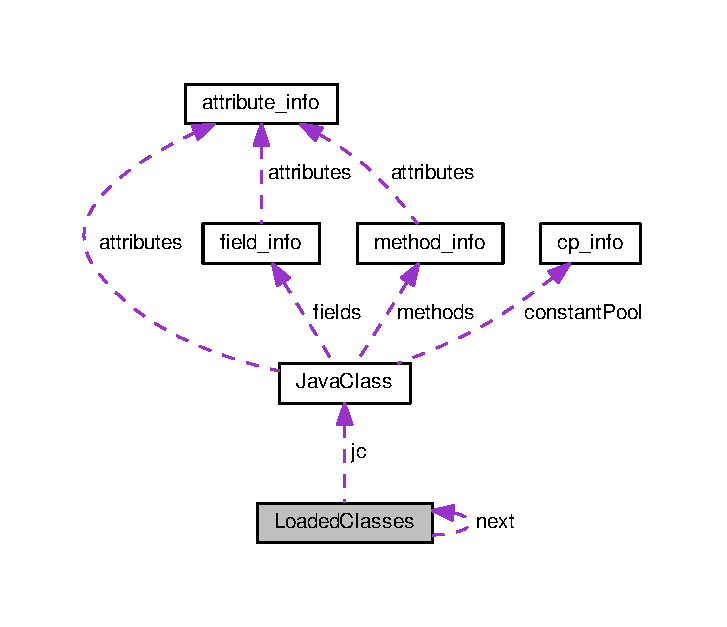
\includegraphics[width=349pt]{structLoadedClasses__coll__graph}
\end{center}
\end{figure}
\subsection*{Campos de Dados}
\begin{DoxyCompactItemize}
\item 
\hyperlink{structJavaClass}{Java\+Class} $\ast$ \hyperlink{structLoadedClasses_a9926f0f305ae1f117b2709b17c9084d8}{jc}
\item 
struct \hyperlink{structLoadedClasses}{Loaded\+Classes} $\ast$ \hyperlink{structLoadedClasses_a66c15555a97e890e2967fac61bb540b8}{next}
\end{DoxyCompactItemize}


\subsection{Documentação dos campos e atributos}
\index{Loaded\+Classes@{Loaded\+Classes}!jc@{jc}}
\index{jc@{jc}!Loaded\+Classes@{Loaded\+Classes}}
\subsubsection[{\texorpdfstring{jc}{jc}}]{\setlength{\rightskip}{0pt plus 5cm}{\bf Java\+Class}$\ast$ Loaded\+Classes\+::jc}\hypertarget{structLoadedClasses_a9926f0f305ae1f117b2709b17c9084d8}{}\label{structLoadedClasses_a9926f0f305ae1f117b2709b17c9084d8}
\index{Loaded\+Classes@{Loaded\+Classes}!next@{next}}
\index{next@{next}!Loaded\+Classes@{Loaded\+Classes}}
\subsubsection[{\texorpdfstring{next}{next}}]{\setlength{\rightskip}{0pt plus 5cm}struct {\bf Loaded\+Classes}$\ast$ Loaded\+Classes\+::next}\hypertarget{structLoadedClasses_a66c15555a97e890e2967fac61bb540b8}{}\label{structLoadedClasses_a66c15555a97e890e2967fac61bb540b8}


A documentação para esta estrutura foi gerada a partir do seguinte ficheiro\+:\begin{DoxyCompactItemize}
\item 
src/\hyperlink{jvm_8h}{jvm.\+h}\end{DoxyCompactItemize}

\hypertarget{structmethod__info}{}\section{Referência à estrutura method\+\_\+info}
\label{structmethod__info}\index{method\+\_\+info@{method\+\_\+info}}


{\ttfamily \#include $<$methods.\+h$>$}



Diagrama de colaboração para method\+\_\+info\+:\nopagebreak
\begin{figure}[H]
\begin{center}
\leavevmode
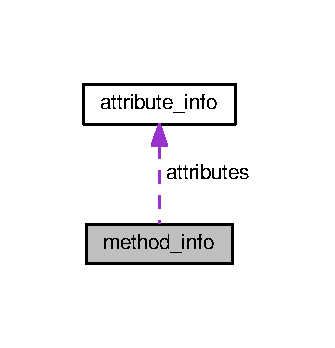
\includegraphics[width=161pt]{structmethod__info__coll__graph}
\end{center}
\end{figure}
\subsection*{Campos de Dados}
\begin{DoxyCompactItemize}
\item 
uint16\+\_\+t \hyperlink{structmethod__info_a8fc68aba419f2617deda879c467f5410}{access\+\_\+flags}
\item 
uint16\+\_\+t \hyperlink{structmethod__info_af0ba3d6d566432e74eed5c37cd998c14}{name\+\_\+index}
\item 
uint16\+\_\+t \hyperlink{structmethod__info_abccd6a5202d4c0ee1be6b89692d0352a}{descriptor\+\_\+index}
\item 
uint16\+\_\+t \hyperlink{structmethod__info_a9e711e4dfb8181f7dce16c6f640ba734}{attributes\+\_\+count}
\item 
\hyperlink{structattribute__info}{attribute\+\_\+info} $\ast$ \hyperlink{structmethod__info_a8ce4caaa03680c91f548558a38647ad8}{attributes}
\end{DoxyCompactItemize}


\subsection{Documentação dos campos e atributos}
\index{method\+\_\+info@{method\+\_\+info}!access\+\_\+flags@{access\+\_\+flags}}
\index{access\+\_\+flags@{access\+\_\+flags}!method\+\_\+info@{method\+\_\+info}}
\subsubsection[{\texorpdfstring{access\+\_\+flags}{access_flags}}]{\setlength{\rightskip}{0pt plus 5cm}uint16\+\_\+t method\+\_\+info\+::access\+\_\+flags}\hypertarget{structmethod__info_a8fc68aba419f2617deda879c467f5410}{}\label{structmethod__info_a8fc68aba419f2617deda879c467f5410}
\index{method\+\_\+info@{method\+\_\+info}!attributes@{attributes}}
\index{attributes@{attributes}!method\+\_\+info@{method\+\_\+info}}
\subsubsection[{\texorpdfstring{attributes}{attributes}}]{\setlength{\rightskip}{0pt plus 5cm}{\bf attribute\+\_\+info}$\ast$ method\+\_\+info\+::attributes}\hypertarget{structmethod__info_a8ce4caaa03680c91f548558a38647ad8}{}\label{structmethod__info_a8ce4caaa03680c91f548558a38647ad8}
\index{method\+\_\+info@{method\+\_\+info}!attributes\+\_\+count@{attributes\+\_\+count}}
\index{attributes\+\_\+count@{attributes\+\_\+count}!method\+\_\+info@{method\+\_\+info}}
\subsubsection[{\texorpdfstring{attributes\+\_\+count}{attributes_count}}]{\setlength{\rightskip}{0pt plus 5cm}uint16\+\_\+t method\+\_\+info\+::attributes\+\_\+count}\hypertarget{structmethod__info_a9e711e4dfb8181f7dce16c6f640ba734}{}\label{structmethod__info_a9e711e4dfb8181f7dce16c6f640ba734}
\index{method\+\_\+info@{method\+\_\+info}!descriptor\+\_\+index@{descriptor\+\_\+index}}
\index{descriptor\+\_\+index@{descriptor\+\_\+index}!method\+\_\+info@{method\+\_\+info}}
\subsubsection[{\texorpdfstring{descriptor\+\_\+index}{descriptor_index}}]{\setlength{\rightskip}{0pt plus 5cm}uint16\+\_\+t method\+\_\+info\+::descriptor\+\_\+index}\hypertarget{structmethod__info_abccd6a5202d4c0ee1be6b89692d0352a}{}\label{structmethod__info_abccd6a5202d4c0ee1be6b89692d0352a}
\index{method\+\_\+info@{method\+\_\+info}!name\+\_\+index@{name\+\_\+index}}
\index{name\+\_\+index@{name\+\_\+index}!method\+\_\+info@{method\+\_\+info}}
\subsubsection[{\texorpdfstring{name\+\_\+index}{name_index}}]{\setlength{\rightskip}{0pt plus 5cm}uint16\+\_\+t method\+\_\+info\+::name\+\_\+index}\hypertarget{structmethod__info_af0ba3d6d566432e74eed5c37cd998c14}{}\label{structmethod__info_af0ba3d6d566432e74eed5c37cd998c14}


A documentação para esta estrutura foi gerada a partir do seguinte ficheiro\+:\begin{DoxyCompactItemize}
\item 
src/\hyperlink{methods_8h}{methods.\+h}\end{DoxyCompactItemize}

\hypertarget{structOperandStack}{}\section{Referência à estrutura Operand\+Stack}
\label{structOperandStack}\index{Operand\+Stack@{Operand\+Stack}}


{\ttfamily \#include $<$operandstack.\+h$>$}



Diagrama de colaboração para Operand\+Stack\+:\nopagebreak
\begin{figure}[H]
\begin{center}
\leavevmode
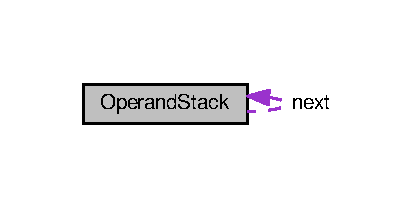
\includegraphics[width=199pt]{structOperandStack__coll__graph}
\end{center}
\end{figure}
\subsection*{Campos de Dados}
\begin{DoxyCompactItemize}
\item 
int32\+\_\+t \hyperlink{structOperandStack_a931d181370bfdb5b41edb8fe488c3b90}{value}
\item 
enum \hyperlink{operandstack_8h_aa4b9b8291a90b1a586c468110fb346a4}{Operand\+Type} \hyperlink{structOperandStack_a757f9fff730b28c1df05b0226d93416f}{type}
\item 
struct \hyperlink{structOperandStack}{Operand\+Stack} $\ast$ \hyperlink{structOperandStack_a6ebcd214896350aa3c1e300ab5ea6f8e}{next}
\end{DoxyCompactItemize}


\subsection{Documentação dos campos e atributos}
\index{Operand\+Stack@{Operand\+Stack}!next@{next}}
\index{next@{next}!Operand\+Stack@{Operand\+Stack}}
\subsubsection[{\texorpdfstring{next}{next}}]{\setlength{\rightskip}{0pt plus 5cm}struct {\bf Operand\+Stack}$\ast$ Operand\+Stack\+::next}\hypertarget{structOperandStack_a6ebcd214896350aa3c1e300ab5ea6f8e}{}\label{structOperandStack_a6ebcd214896350aa3c1e300ab5ea6f8e}
\index{Operand\+Stack@{Operand\+Stack}!type@{type}}
\index{type@{type}!Operand\+Stack@{Operand\+Stack}}
\subsubsection[{\texorpdfstring{type}{type}}]{\setlength{\rightskip}{0pt plus 5cm}enum {\bf Operand\+Type} Operand\+Stack\+::type}\hypertarget{structOperandStack_a757f9fff730b28c1df05b0226d93416f}{}\label{structOperandStack_a757f9fff730b28c1df05b0226d93416f}
\index{Operand\+Stack@{Operand\+Stack}!value@{value}}
\index{value@{value}!Operand\+Stack@{Operand\+Stack}}
\subsubsection[{\texorpdfstring{value}{value}}]{\setlength{\rightskip}{0pt plus 5cm}int32\+\_\+t Operand\+Stack\+::value}\hypertarget{structOperandStack_a931d181370bfdb5b41edb8fe488c3b90}{}\label{structOperandStack_a931d181370bfdb5b41edb8fe488c3b90}


A documentação para esta estrutura foi gerada a partir do seguinte ficheiro\+:\begin{DoxyCompactItemize}
\item 
src/\hyperlink{operandstack_8h}{operandstack.\+h}\end{DoxyCompactItemize}

\chapter{Documentação do ficheiro}
\hypertarget{attributes_8c}{}\section{Referência ao ficheiro src/attributes.c}
\label{attributes_8c}\index{src/attributes.\+c@{src/attributes.\+c}}
{\ttfamily \#include \char`\"{}attributes.\+h\char`\"{}}\\*
{\ttfamily \#include \char`\"{}readfunctions.\+h\char`\"{}}\\*
{\ttfamily \#include \char`\"{}utf8.\+h\char`\"{}}\\*
{\ttfamily \#include \char`\"{}opcodes.\+h\char`\"{}}\\*
{\ttfamily \#include $<$stdlib.\+h$>$}\\*
{\ttfamily \#include $<$inttypes.\+h$>$}\\*
Diagrama de dependências de inclusão para attributes.\+c\+:\nopagebreak
\begin{figure}[H]
\begin{center}
\leavevmode
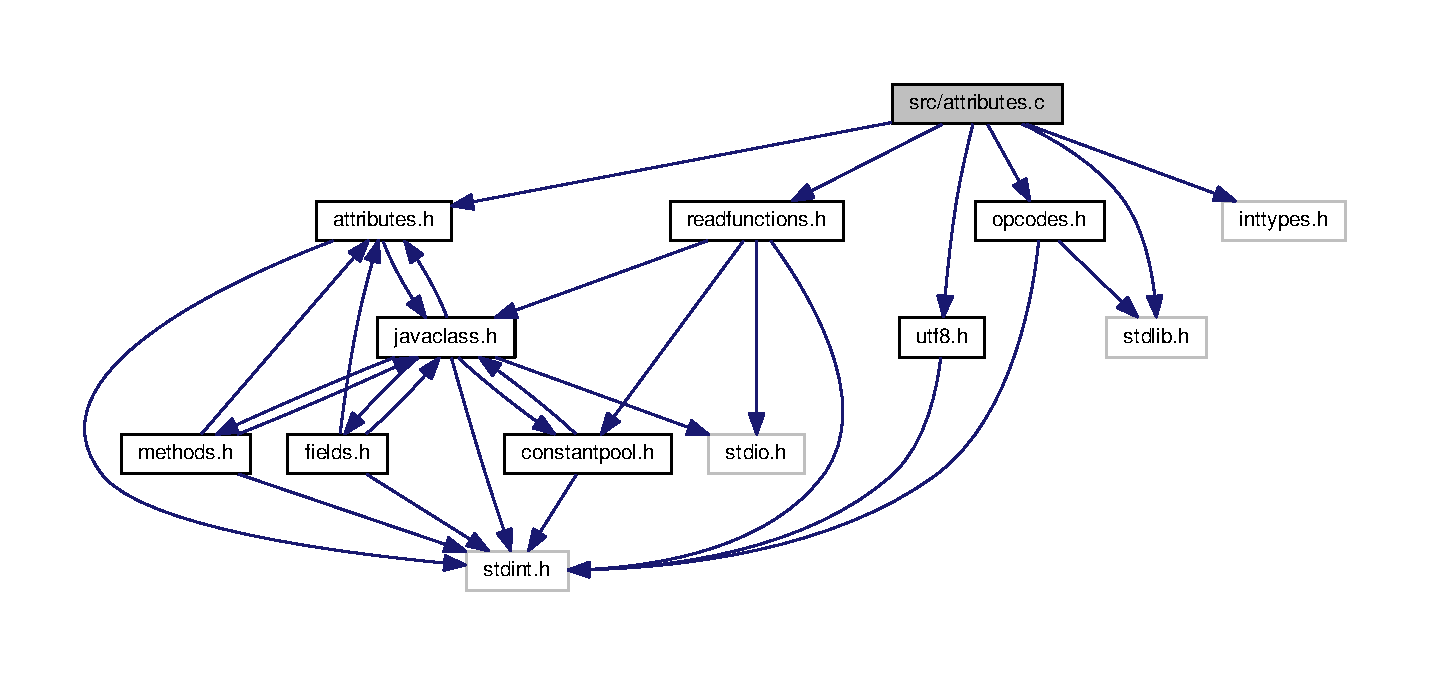
\includegraphics[width=350pt]{attributes_8c__incl}
\end{center}
\end{figure}
\subsection*{Macros}
\begin{DoxyCompactItemize}
\item 
\#define \hyperlink{attributes_8c_a1a4c6b25eeb17e81e6376d4a6383c158}{D\+E\+C\+L\+A\+R\+E\+\_\+\+A\+T\+T\+R\+\_\+\+F\+U\+N\+CS}(attr)
\item 
\#define \hyperlink{attributes_8c_afa2f48f44da881b9d32c1a7d1e4db4ab}{I\+F\+\_\+\+A\+T\+T\+R\+\_\+\+C\+H\+E\+CK}(name)
\item 
\#define \hyperlink{attributes_8c_acc32225b9d3eb1107b48de3cd4539075}{O\+P\+C\+O\+D\+E\+\_\+\+I\+N\+T\+E\+R\+V\+AL}(begin,  end)~(opcode $>$= opcode\+\_\+\#\#begin \&\& opcode $<$= opcode\+\_\+\#\#end)
\item 
\#define \hyperlink{attributes_8c_ab757e29ce18ed03f73c4b81a869e4b9a}{N\+E\+X\+T\+B\+Y\+TE}~($\ast$(info-\/$>$code + ++code\+\_\+offset))
\item 
\#define \hyperlink{attributes_8c_acd9132a8a41b59ee57e8326b1f516fa9}{A\+T\+T\+R\+\_\+\+C\+A\+SE}(attr)~case A\+T\+T\+R\+\_\+\#\#attr\+: free\+Attribute\#\#attr(entry); return;
\item 
\#define \hyperlink{attributes_8c_acd9132a8a41b59ee57e8326b1f516fa9}{A\+T\+T\+R\+\_\+\+C\+A\+SE}(attr)~case A\+T\+T\+R\+\_\+\#\#attr\+: \hyperlink{attributes_8h_aee295c33031c2ab941c9260654010db7}{print\+Attribute}\#\#attr(jc, entry, identation\+Level); break;
\end{DoxyCompactItemize}
\subsection*{Funções}
\begin{DoxyCompactItemize}
\item 
char \hyperlink{attributes_8c_a0aab7731ade76c16c2ff8b3bef1111d1}{read\+Attribute} (\hyperlink{structJavaClass}{Java\+Class} $\ast$jc, \hyperlink{structattribute__info}{attribute\+\_\+info} $\ast$entry)
\item 
void \hyperlink{attributes_8c_a01657db1f2f2e478b93e5329c666901e}{ident} (int level)
\item 
uint8\+\_\+t \hyperlink{attributes_8c_a5e568e134ff6fb82b263565076da0432}{read\+Attribute\+Deprecated} (\hyperlink{structJavaClass}{Java\+Class} $\ast$jc, \hyperlink{structattribute__info}{attribute\+\_\+info} $\ast$entry)
\item 
void \hyperlink{attributes_8c_ad80e46006ae1ca8e80f84735d331fc18}{print\+Attribute\+Deprecated} (\hyperlink{structJavaClass}{Java\+Class} $\ast$jc, \hyperlink{structattribute__info}{attribute\+\_\+info} $\ast$entry, int identation\+Level)
\item 
void \hyperlink{attributes_8c_ac122c1bdf1457e87c2cbdb8ec5ca1625}{free\+Attribute\+Deprecated} (\hyperlink{structattribute__info}{attribute\+\_\+info} $\ast$entry)
\item 
uint8\+\_\+t \hyperlink{attributes_8c_ac07fa201160b522b15c7353b4ff2ed44}{read\+Attribute\+Constant\+Value} (\hyperlink{structJavaClass}{Java\+Class} $\ast$jc, \hyperlink{structattribute__info}{attribute\+\_\+info} $\ast$entry)
\item 
void \hyperlink{attributes_8c_a5abd76089f5e6794d1ecc98cea55f158}{print\+Attribute\+Constant\+Value} (\hyperlink{structJavaClass}{Java\+Class} $\ast$jc, \hyperlink{structattribute__info}{attribute\+\_\+info} $\ast$entry, int identation\+Level)
\item 
void \hyperlink{attributes_8c_a3b65b1bc8966d4ad3a18e52ad7a3586b}{free\+Attribute\+Constant\+Value} (\hyperlink{structattribute__info}{attribute\+\_\+info} $\ast$entry)
\item 
uint8\+\_\+t \hyperlink{attributes_8c_a43bfb8cf040e623ccae73943a943a7f8}{read\+Attribute\+Source\+File} (\hyperlink{structJavaClass}{Java\+Class} $\ast$jc, \hyperlink{structattribute__info}{attribute\+\_\+info} $\ast$entry)
\item 
void \hyperlink{attributes_8c_a7566e0f5a2ba5992f6e8f84a7b5d0b8b}{print\+Attribute\+Source\+File} (\hyperlink{structJavaClass}{Java\+Class} $\ast$jc, \hyperlink{structattribute__info}{attribute\+\_\+info} $\ast$entry, int identation\+Level)
\item 
void \hyperlink{attributes_8c_ae0485d0a13108130dd232c001a4502fe}{free\+Attribute\+Source\+File} (\hyperlink{structattribute__info}{attribute\+\_\+info} $\ast$entry)
\item 
uint8\+\_\+t \hyperlink{attributes_8c_a7af979b9e909d50393f578f9cf230fae}{read\+Attribute\+Inner\+Classes} (\hyperlink{structJavaClass}{Java\+Class} $\ast$jc, \hyperlink{structattribute__info}{attribute\+\_\+info} $\ast$entry)
\item 
void \hyperlink{attributes_8c_a6c90c1dd47892d19d581ef9fcac24698}{print\+Attribute\+Inner\+Classes} (\hyperlink{structJavaClass}{Java\+Class} $\ast$jc, \hyperlink{structattribute__info}{attribute\+\_\+info} $\ast$entry, int identation\+Level)
\item 
void \hyperlink{attributes_8c_a21f76b789715d6055265e69dc63e4eeb}{free\+Attribute\+Inner\+Classes} (\hyperlink{structattribute__info}{attribute\+\_\+info} $\ast$entry)
\item 
uint8\+\_\+t \hyperlink{attributes_8c_a837af1196cf968ff688539be299648d5}{read\+Attribute\+Line\+Number\+Table} (\hyperlink{structJavaClass}{Java\+Class} $\ast$jc, \hyperlink{structattribute__info}{attribute\+\_\+info} $\ast$entry)
\item 
void \hyperlink{attributes_8c_a8c510d03555d15e558997e15e000c40f}{print\+Attribute\+Line\+Number\+Table} (\hyperlink{structJavaClass}{Java\+Class} $\ast$jc, \hyperlink{structattribute__info}{attribute\+\_\+info} $\ast$entry, int identation\+Level)
\item 
void \hyperlink{attributes_8c_af8c25d4cde9d8421cd4fefc8543d1ec7}{free\+Attribute\+Line\+Number\+Table} (\hyperlink{structattribute__info}{attribute\+\_\+info} $\ast$entry)
\item 
uint8\+\_\+t \hyperlink{attributes_8c_af3a1b04442990e1699afc5b2592c4c93}{read\+Attribute\+Code} (\hyperlink{structJavaClass}{Java\+Class} $\ast$jc, \hyperlink{structattribute__info}{attribute\+\_\+info} $\ast$entry)
\item 
void \hyperlink{attributes_8c_ae588cbde97553719c8b8612e8e42f4b4}{print\+Attribute\+Code} (\hyperlink{structJavaClass}{Java\+Class} $\ast$jc, \hyperlink{structattribute__info}{attribute\+\_\+info} $\ast$entry, int identation\+Level)
\item 
void \hyperlink{attributes_8c_a2e8c24440f4c49b6dd8a19cd9fe584c0}{free\+Attribute\+Code} (\hyperlink{structattribute__info}{attribute\+\_\+info} $\ast$entry)
\item 
uint8\+\_\+t \hyperlink{attributes_8c_a1aabfbdd22c8a11214ee3db33624b734}{read\+Attribute\+Exceptions} (\hyperlink{structJavaClass}{Java\+Class} $\ast$jc, \hyperlink{structattribute__info}{attribute\+\_\+info} $\ast$entry)
\item 
void \hyperlink{attributes_8c_a1aeef532497a7cc1a3dee89d104bd725}{print\+Attribute\+Exceptions} (\hyperlink{structJavaClass}{Java\+Class} $\ast$jc, \hyperlink{structattribute__info}{attribute\+\_\+info} $\ast$entry, int identation\+Level)
\item 
void \hyperlink{attributes_8c_a47063751996bba4e939a7d2bcebd2b10}{free\+Attribute\+Exceptions} (\hyperlink{structattribute__info}{attribute\+\_\+info} $\ast$entry)
\item 
void \hyperlink{attributes_8c_a136bdfadd787ebd62f1c721f99270cc9}{free\+Attribute\+Info} (\hyperlink{structattribute__info}{attribute\+\_\+info} $\ast$entry)
\item 
void \hyperlink{attributes_8c_aee295c33031c2ab941c9260654010db7}{print\+Attribute} (\hyperlink{structJavaClass}{Java\+Class} $\ast$jc, \hyperlink{structattribute__info}{attribute\+\_\+info} $\ast$entry, int identation\+Level)
\item 
void \hyperlink{attributes_8c_ae04e26b66957c879139f8a82e463674a}{print\+All\+Attributes} (\hyperlink{structJavaClass}{Java\+Class} $\ast$jc)
\item 
\hyperlink{structattribute__info}{attribute\+\_\+info} $\ast$ \hyperlink{attributes_8c_ae3ce1b33741046741c90a6f5592911a5}{get\+Attribute\+By\+Type} (\hyperlink{structattribute__info}{attribute\+\_\+info} $\ast$attributes, uint16\+\_\+t attributes\+\_\+length, enum \hyperlink{attributes_8h_a349a9cde14be8097df865ba0469c0ab2}{Attribute\+Type} type)
\end{DoxyCompactItemize}


\subsection{Documentação das macros}
\index{attributes.\+c@{attributes.\+c}!A\+T\+T\+R\+\_\+\+C\+A\+SE@{A\+T\+T\+R\+\_\+\+C\+A\+SE}}
\index{A\+T\+T\+R\+\_\+\+C\+A\+SE@{A\+T\+T\+R\+\_\+\+C\+A\+SE}!attributes.\+c@{attributes.\+c}}
\subsubsection[{\texorpdfstring{A\+T\+T\+R\+\_\+\+C\+A\+SE}{ATTR_CASE}}]{\setlength{\rightskip}{0pt plus 5cm}\#define A\+T\+T\+R\+\_\+\+C\+A\+SE(
\begin{DoxyParamCaption}
\item[{}]{attr}
\end{DoxyParamCaption}
)~case A\+T\+T\+R\+\_\+\#\#attr\+: free\+Attribute\#\#attr(entry); return;}\hypertarget{attributes_8c_acd9132a8a41b59ee57e8326b1f516fa9}{}\label{attributes_8c_acd9132a8a41b59ee57e8326b1f516fa9}
\index{attributes.\+c@{attributes.\+c}!A\+T\+T\+R\+\_\+\+C\+A\+SE@{A\+T\+T\+R\+\_\+\+C\+A\+SE}}
\index{A\+T\+T\+R\+\_\+\+C\+A\+SE@{A\+T\+T\+R\+\_\+\+C\+A\+SE}!attributes.\+c@{attributes.\+c}}
\subsubsection[{\texorpdfstring{A\+T\+T\+R\+\_\+\+C\+A\+SE}{ATTR_CASE}}]{\setlength{\rightskip}{0pt plus 5cm}\#define A\+T\+T\+R\+\_\+\+C\+A\+SE(
\begin{DoxyParamCaption}
\item[{}]{attr}
\end{DoxyParamCaption}
)~case A\+T\+T\+R\+\_\+\#\#attr\+: {\bf print\+Attribute}\#\#attr(jc, entry, identation\+Level); break;}\hypertarget{attributes_8c_acd9132a8a41b59ee57e8326b1f516fa9}{}\label{attributes_8c_acd9132a8a41b59ee57e8326b1f516fa9}
\index{attributes.\+c@{attributes.\+c}!D\+E\+C\+L\+A\+R\+E\+\_\+\+A\+T\+T\+R\+\_\+\+F\+U\+N\+CS@{D\+E\+C\+L\+A\+R\+E\+\_\+\+A\+T\+T\+R\+\_\+\+F\+U\+N\+CS}}
\index{D\+E\+C\+L\+A\+R\+E\+\_\+\+A\+T\+T\+R\+\_\+\+F\+U\+N\+CS@{D\+E\+C\+L\+A\+R\+E\+\_\+\+A\+T\+T\+R\+\_\+\+F\+U\+N\+CS}!attributes.\+c@{attributes.\+c}}
\subsubsection[{\texorpdfstring{D\+E\+C\+L\+A\+R\+E\+\_\+\+A\+T\+T\+R\+\_\+\+F\+U\+N\+CS}{DECLARE_ATTR_FUNCS}}]{\setlength{\rightskip}{0pt plus 5cm}\#define D\+E\+C\+L\+A\+R\+E\+\_\+\+A\+T\+T\+R\+\_\+\+F\+U\+N\+CS(
\begin{DoxyParamCaption}
\item[{}]{attr}
\end{DoxyParamCaption}
)}\hypertarget{attributes_8c_a1a4c6b25eeb17e81e6376d4a6383c158}{}\label{attributes_8c_a1a4c6b25eeb17e81e6376d4a6383c158}
{\bfseries Valor\+:}
\begin{DoxyCode}
uint8\_t \hyperlink{attributes_8c_a0aab7731ade76c16c2ff8b3bef1111d1}{readAttribute}##attr(\hyperlink{structJavaClass}{JavaClass}* jc, \hyperlink{structattribute__info}{attribute\_info}* entry); \(\backslash\)
    void \hyperlink{attributes_8c_aee295c33031c2ab941c9260654010db7}{printAttribute}##attr(\hyperlink{structJavaClass}{JavaClass}* jc, 
      \hyperlink{structattribute__info}{attribute\_info}* entry, \textcolor{keywordtype}{int} identationLevel); \(\backslash\)
    void freeAttribute##attr(\hyperlink{structattribute__info}{attribute\_info}* entry);
\end{DoxyCode}
\index{attributes.\+c@{attributes.\+c}!I\+F\+\_\+\+A\+T\+T\+R\+\_\+\+C\+H\+E\+CK@{I\+F\+\_\+\+A\+T\+T\+R\+\_\+\+C\+H\+E\+CK}}
\index{I\+F\+\_\+\+A\+T\+T\+R\+\_\+\+C\+H\+E\+CK@{I\+F\+\_\+\+A\+T\+T\+R\+\_\+\+C\+H\+E\+CK}!attributes.\+c@{attributes.\+c}}
\subsubsection[{\texorpdfstring{I\+F\+\_\+\+A\+T\+T\+R\+\_\+\+C\+H\+E\+CK}{IF_ATTR_CHECK}}]{\setlength{\rightskip}{0pt plus 5cm}\#define I\+F\+\_\+\+A\+T\+T\+R\+\_\+\+C\+H\+E\+CK(
\begin{DoxyParamCaption}
\item[{}]{name}
\end{DoxyParamCaption}
)}\hypertarget{attributes_8c_afa2f48f44da881b9d32c1a7d1e4db4ab}{}\label{attributes_8c_afa2f48f44da881b9d32c1a7d1e4db4ab}
{\bfseries Valor\+:}
\begin{DoxyCode}
\textcolor{keywordflow}{if} (\hyperlink{utf8_8c_a317c1d4f6b0e4b61b5f99baf9d673a8e}{cmp\_UTF8\_Ascii}(cp->Utf8.bytes, cp->Utf8.length, (uint8\_t*)#name, \textcolor{keyword}{sizeof}(#name) - 1)) \{ \(\backslash\)
            entry->attributeType = ATTR\_##name; \(\backslash\)
            result = \hyperlink{attributes_8c_a0aab7731ade76c16c2ff8b3bef1111d1}{readAttribute}##name(jc, entry); \(\backslash\)
        \}
\end{DoxyCode}
\index{attributes.\+c@{attributes.\+c}!N\+E\+X\+T\+B\+Y\+TE@{N\+E\+X\+T\+B\+Y\+TE}}
\index{N\+E\+X\+T\+B\+Y\+TE@{N\+E\+X\+T\+B\+Y\+TE}!attributes.\+c@{attributes.\+c}}
\subsubsection[{\texorpdfstring{N\+E\+X\+T\+B\+Y\+TE}{NEXTBYTE}}]{\setlength{\rightskip}{0pt plus 5cm}\#define N\+E\+X\+T\+B\+Y\+TE~($\ast$(info-\/$>$code + ++code\+\_\+offset))}\hypertarget{attributes_8c_ab757e29ce18ed03f73c4b81a869e4b9a}{}\label{attributes_8c_ab757e29ce18ed03f73c4b81a869e4b9a}
\index{attributes.\+c@{attributes.\+c}!O\+P\+C\+O\+D\+E\+\_\+\+I\+N\+T\+E\+R\+V\+AL@{O\+P\+C\+O\+D\+E\+\_\+\+I\+N\+T\+E\+R\+V\+AL}}
\index{O\+P\+C\+O\+D\+E\+\_\+\+I\+N\+T\+E\+R\+V\+AL@{O\+P\+C\+O\+D\+E\+\_\+\+I\+N\+T\+E\+R\+V\+AL}!attributes.\+c@{attributes.\+c}}
\subsubsection[{\texorpdfstring{O\+P\+C\+O\+D\+E\+\_\+\+I\+N\+T\+E\+R\+V\+AL}{OPCODE_INTERVAL}}]{\setlength{\rightskip}{0pt plus 5cm}\#define O\+P\+C\+O\+D\+E\+\_\+\+I\+N\+T\+E\+R\+V\+AL(
\begin{DoxyParamCaption}
\item[{}]{begin, }
\item[{}]{end}
\end{DoxyParamCaption}
)~(opcode $>$= opcode\+\_\+\#\#begin \&\& opcode $<$= opcode\+\_\+\#\#end)}\hypertarget{attributes_8c_acc32225b9d3eb1107b48de3cd4539075}{}\label{attributes_8c_acc32225b9d3eb1107b48de3cd4539075}


\subsection{Documentação das funções}
\index{attributes.\+c@{attributes.\+c}!free\+Attribute\+Code@{free\+Attribute\+Code}}
\index{free\+Attribute\+Code@{free\+Attribute\+Code}!attributes.\+c@{attributes.\+c}}
\subsubsection[{\texorpdfstring{free\+Attribute\+Code(attribute\+\_\+info $\ast$entry)}{freeAttributeCode(attribute_info *entry)}}]{\setlength{\rightskip}{0pt plus 5cm}void free\+Attribute\+Code (
\begin{DoxyParamCaption}
\item[{{\bf attribute\+\_\+info} $\ast$}]{entry}
\end{DoxyParamCaption}
)}\hypertarget{attributes_8c_a2e8c24440f4c49b6dd8a19cd9fe584c0}{}\label{attributes_8c_a2e8c24440f4c49b6dd8a19cd9fe584c0}
\index{attributes.\+c@{attributes.\+c}!free\+Attribute\+Constant\+Value@{free\+Attribute\+Constant\+Value}}
\index{free\+Attribute\+Constant\+Value@{free\+Attribute\+Constant\+Value}!attributes.\+c@{attributes.\+c}}
\subsubsection[{\texorpdfstring{free\+Attribute\+Constant\+Value(attribute\+\_\+info $\ast$entry)}{freeAttributeConstantValue(attribute_info *entry)}}]{\setlength{\rightskip}{0pt plus 5cm}void free\+Attribute\+Constant\+Value (
\begin{DoxyParamCaption}
\item[{{\bf attribute\+\_\+info} $\ast$}]{entry}
\end{DoxyParamCaption}
)}\hypertarget{attributes_8c_a3b65b1bc8966d4ad3a18e52ad7a3586b}{}\label{attributes_8c_a3b65b1bc8966d4ad3a18e52ad7a3586b}
\index{attributes.\+c@{attributes.\+c}!free\+Attribute\+Deprecated@{free\+Attribute\+Deprecated}}
\index{free\+Attribute\+Deprecated@{free\+Attribute\+Deprecated}!attributes.\+c@{attributes.\+c}}
\subsubsection[{\texorpdfstring{free\+Attribute\+Deprecated(attribute\+\_\+info $\ast$entry)}{freeAttributeDeprecated(attribute_info *entry)}}]{\setlength{\rightskip}{0pt plus 5cm}void free\+Attribute\+Deprecated (
\begin{DoxyParamCaption}
\item[{{\bf attribute\+\_\+info} $\ast$}]{entry}
\end{DoxyParamCaption}
)}\hypertarget{attributes_8c_ac122c1bdf1457e87c2cbdb8ec5ca1625}{}\label{attributes_8c_ac122c1bdf1457e87c2cbdb8ec5ca1625}
\index{attributes.\+c@{attributes.\+c}!free\+Attribute\+Exceptions@{free\+Attribute\+Exceptions}}
\index{free\+Attribute\+Exceptions@{free\+Attribute\+Exceptions}!attributes.\+c@{attributes.\+c}}
\subsubsection[{\texorpdfstring{free\+Attribute\+Exceptions(attribute\+\_\+info $\ast$entry)}{freeAttributeExceptions(attribute_info *entry)}}]{\setlength{\rightskip}{0pt plus 5cm}void free\+Attribute\+Exceptions (
\begin{DoxyParamCaption}
\item[{{\bf attribute\+\_\+info} $\ast$}]{entry}
\end{DoxyParamCaption}
)}\hypertarget{attributes_8c_a47063751996bba4e939a7d2bcebd2b10}{}\label{attributes_8c_a47063751996bba4e939a7d2bcebd2b10}
\index{attributes.\+c@{attributes.\+c}!free\+Attribute\+Info@{free\+Attribute\+Info}}
\index{free\+Attribute\+Info@{free\+Attribute\+Info}!attributes.\+c@{attributes.\+c}}
\subsubsection[{\texorpdfstring{free\+Attribute\+Info(attribute\+\_\+info $\ast$entry)}{freeAttributeInfo(attribute_info *entry)}}]{\setlength{\rightskip}{0pt plus 5cm}void free\+Attribute\+Info (
\begin{DoxyParamCaption}
\item[{{\bf attribute\+\_\+info} $\ast$}]{entry}
\end{DoxyParamCaption}
)}\hypertarget{attributes_8c_a136bdfadd787ebd62f1c721f99270cc9}{}\label{attributes_8c_a136bdfadd787ebd62f1c721f99270cc9}


Este é o diagrama das funções que utilizam esta função\+:\nopagebreak
\begin{figure}[H]
\begin{center}
\leavevmode
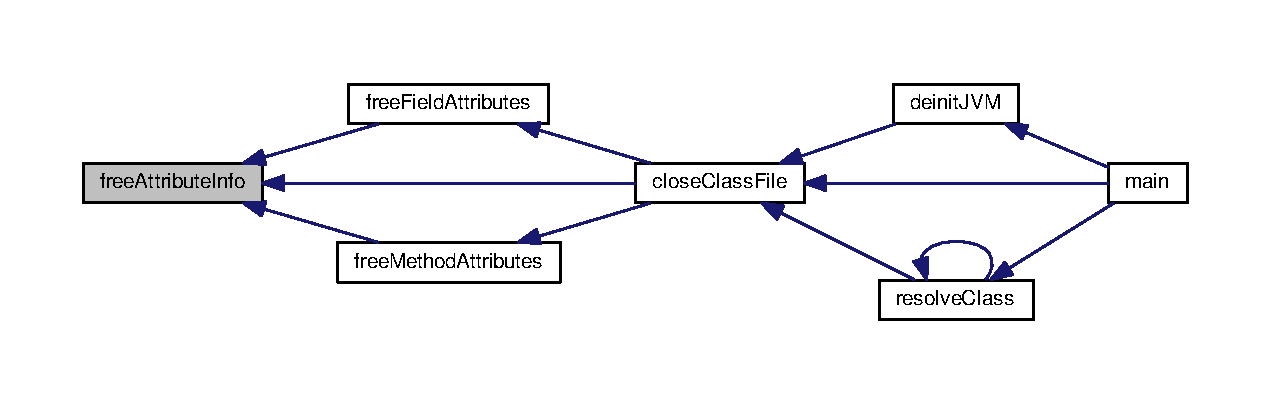
\includegraphics[width=350pt]{attributes_8c_a136bdfadd787ebd62f1c721f99270cc9_icgraph}
\end{center}
\end{figure}


\index{attributes.\+c@{attributes.\+c}!free\+Attribute\+Inner\+Classes@{free\+Attribute\+Inner\+Classes}}
\index{free\+Attribute\+Inner\+Classes@{free\+Attribute\+Inner\+Classes}!attributes.\+c@{attributes.\+c}}
\subsubsection[{\texorpdfstring{free\+Attribute\+Inner\+Classes(attribute\+\_\+info $\ast$entry)}{freeAttributeInnerClasses(attribute_info *entry)}}]{\setlength{\rightskip}{0pt plus 5cm}void free\+Attribute\+Inner\+Classes (
\begin{DoxyParamCaption}
\item[{{\bf attribute\+\_\+info} $\ast$}]{entry}
\end{DoxyParamCaption}
)}\hypertarget{attributes_8c_a21f76b789715d6055265e69dc63e4eeb}{}\label{attributes_8c_a21f76b789715d6055265e69dc63e4eeb}
\index{attributes.\+c@{attributes.\+c}!free\+Attribute\+Line\+Number\+Table@{free\+Attribute\+Line\+Number\+Table}}
\index{free\+Attribute\+Line\+Number\+Table@{free\+Attribute\+Line\+Number\+Table}!attributes.\+c@{attributes.\+c}}
\subsubsection[{\texorpdfstring{free\+Attribute\+Line\+Number\+Table(attribute\+\_\+info $\ast$entry)}{freeAttributeLineNumberTable(attribute_info *entry)}}]{\setlength{\rightskip}{0pt plus 5cm}void free\+Attribute\+Line\+Number\+Table (
\begin{DoxyParamCaption}
\item[{{\bf attribute\+\_\+info} $\ast$}]{entry}
\end{DoxyParamCaption}
)}\hypertarget{attributes_8c_af8c25d4cde9d8421cd4fefc8543d1ec7}{}\label{attributes_8c_af8c25d4cde9d8421cd4fefc8543d1ec7}
\index{attributes.\+c@{attributes.\+c}!free\+Attribute\+Source\+File@{free\+Attribute\+Source\+File}}
\index{free\+Attribute\+Source\+File@{free\+Attribute\+Source\+File}!attributes.\+c@{attributes.\+c}}
\subsubsection[{\texorpdfstring{free\+Attribute\+Source\+File(attribute\+\_\+info $\ast$entry)}{freeAttributeSourceFile(attribute_info *entry)}}]{\setlength{\rightskip}{0pt plus 5cm}void free\+Attribute\+Source\+File (
\begin{DoxyParamCaption}
\item[{{\bf attribute\+\_\+info} $\ast$}]{entry}
\end{DoxyParamCaption}
)}\hypertarget{attributes_8c_ae0485d0a13108130dd232c001a4502fe}{}\label{attributes_8c_ae0485d0a13108130dd232c001a4502fe}
\index{attributes.\+c@{attributes.\+c}!get\+Attribute\+By\+Type@{get\+Attribute\+By\+Type}}
\index{get\+Attribute\+By\+Type@{get\+Attribute\+By\+Type}!attributes.\+c@{attributes.\+c}}
\subsubsection[{\texorpdfstring{get\+Attribute\+By\+Type(attribute\+\_\+info $\ast$attributes, uint16\+\_\+t attributes\+\_\+length, enum Attribute\+Type type)}{getAttributeByType(attribute_info *attributes, uint16_t attributes_length, enum AttributeType type)}}]{\setlength{\rightskip}{0pt plus 5cm}{\bf attribute\+\_\+info}$\ast$ get\+Attribute\+By\+Type (
\begin{DoxyParamCaption}
\item[{{\bf attribute\+\_\+info} $\ast$}]{attributes, }
\item[{uint16\+\_\+t}]{attributes\+\_\+length, }
\item[{enum {\bf Attribute\+Type}}]{type}
\end{DoxyParamCaption}
)}\hypertarget{attributes_8c_ae3ce1b33741046741c90a6f5592911a5}{}\label{attributes_8c_ae3ce1b33741046741c90a6f5592911a5}


Este é o diagrama das funções que utilizam esta função\+:\nopagebreak
\begin{figure}[H]
\begin{center}
\leavevmode
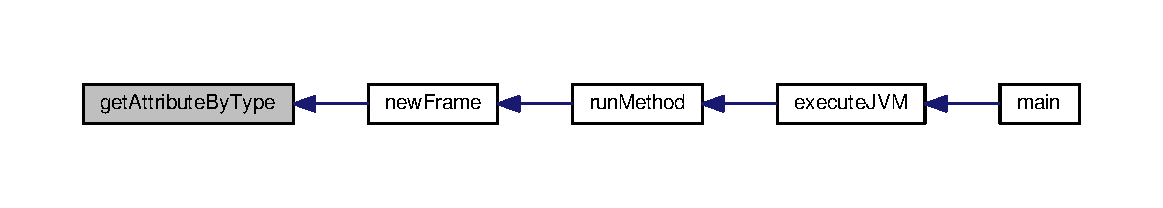
\includegraphics[width=350pt]{attributes_8c_ae3ce1b33741046741c90a6f5592911a5_icgraph}
\end{center}
\end{figure}


\index{attributes.\+c@{attributes.\+c}!ident@{ident}}
\index{ident@{ident}!attributes.\+c@{attributes.\+c}}
\subsubsection[{\texorpdfstring{ident(int level)}{ident(int level)}}]{\setlength{\rightskip}{0pt plus 5cm}void ident (
\begin{DoxyParamCaption}
\item[{int}]{level}
\end{DoxyParamCaption}
)}\hypertarget{attributes_8c_a01657db1f2f2e478b93e5329c666901e}{}\label{attributes_8c_a01657db1f2f2e478b93e5329c666901e}


Este é o diagrama das funções que utilizam esta função\+:\nopagebreak
\begin{figure}[H]
\begin{center}
\leavevmode
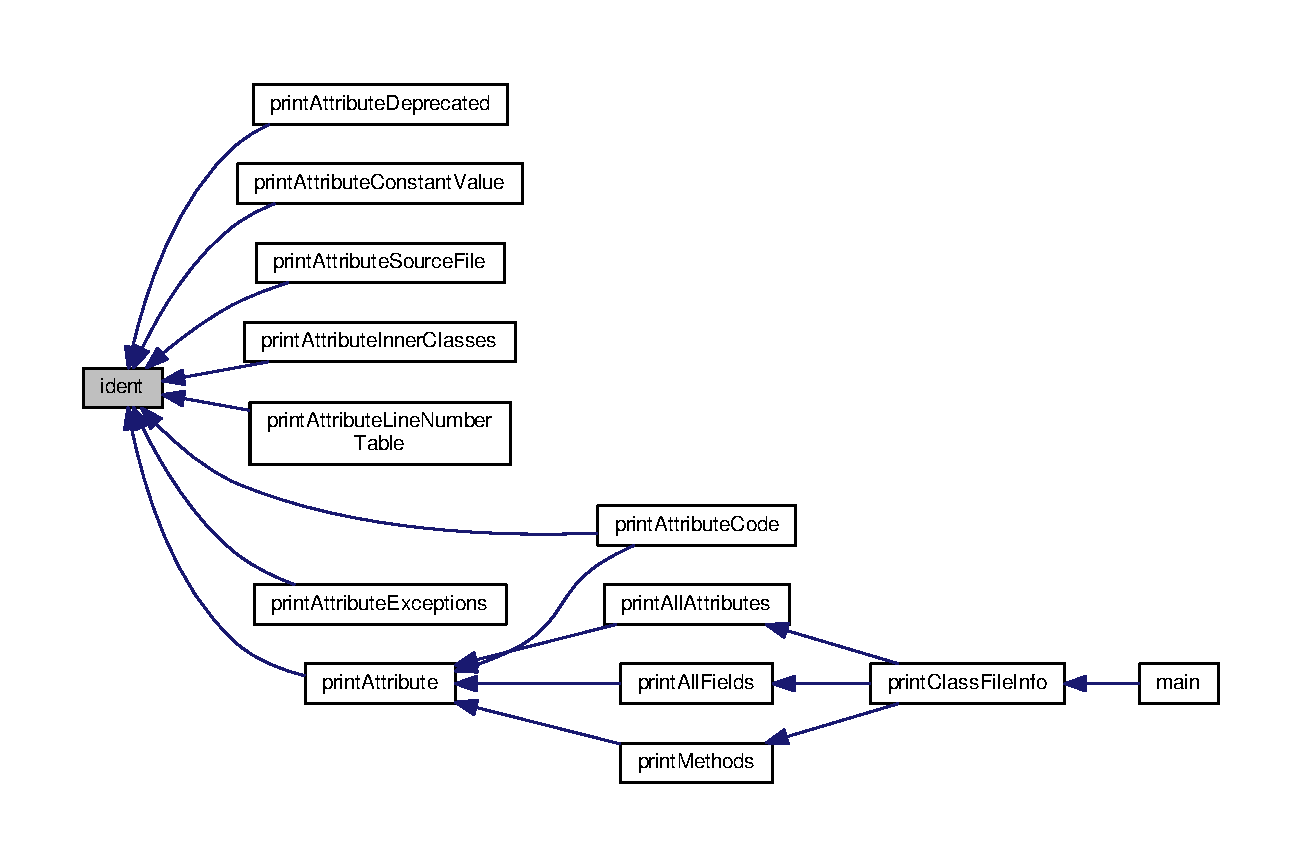
\includegraphics[width=350pt]{attributes_8c_a01657db1f2f2e478b93e5329c666901e_icgraph}
\end{center}
\end{figure}


\index{attributes.\+c@{attributes.\+c}!print\+All\+Attributes@{print\+All\+Attributes}}
\index{print\+All\+Attributes@{print\+All\+Attributes}!attributes.\+c@{attributes.\+c}}
\subsubsection[{\texorpdfstring{print\+All\+Attributes(\+Java\+Class $\ast$jc)}{printAllAttributes(JavaClass *jc)}}]{\setlength{\rightskip}{0pt plus 5cm}void print\+All\+Attributes (
\begin{DoxyParamCaption}
\item[{{\bf Java\+Class} $\ast$}]{jc}
\end{DoxyParamCaption}
)}\hypertarget{attributes_8c_ae04e26b66957c879139f8a82e463674a}{}\label{attributes_8c_ae04e26b66957c879139f8a82e463674a}


Grafo de chamadas desta função\+:\nopagebreak
\begin{figure}[H]
\begin{center}
\leavevmode
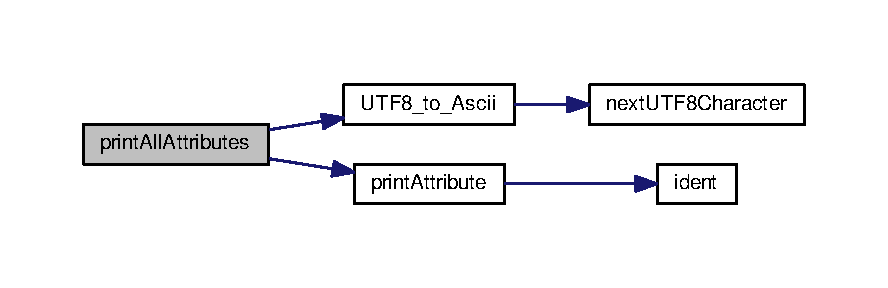
\includegraphics[width=350pt]{attributes_8c_ae04e26b66957c879139f8a82e463674a_cgraph}
\end{center}
\end{figure}




Este é o diagrama das funções que utilizam esta função\+:\nopagebreak
\begin{figure}[H]
\begin{center}
\leavevmode
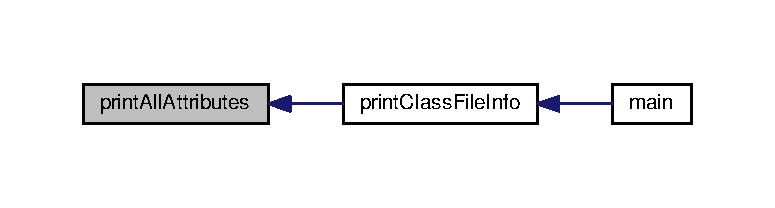
\includegraphics[width=350pt]{attributes_8c_ae04e26b66957c879139f8a82e463674a_icgraph}
\end{center}
\end{figure}


\index{attributes.\+c@{attributes.\+c}!print\+Attribute@{print\+Attribute}}
\index{print\+Attribute@{print\+Attribute}!attributes.\+c@{attributes.\+c}}
\subsubsection[{\texorpdfstring{print\+Attribute(\+Java\+Class $\ast$jc, attribute\+\_\+info $\ast$entry, int identation\+Level)}{printAttribute(JavaClass *jc, attribute_info *entry, int identationLevel)}}]{\setlength{\rightskip}{0pt plus 5cm}void print\+Attribute (
\begin{DoxyParamCaption}
\item[{{\bf Java\+Class} $\ast$}]{jc, }
\item[{{\bf attribute\+\_\+info} $\ast$}]{entry, }
\item[{int}]{identation\+Level}
\end{DoxyParamCaption}
)}\hypertarget{attributes_8c_aee295c33031c2ab941c9260654010db7}{}\label{attributes_8c_aee295c33031c2ab941c9260654010db7}


Grafo de chamadas desta função\+:\nopagebreak
\begin{figure}[H]
\begin{center}
\leavevmode
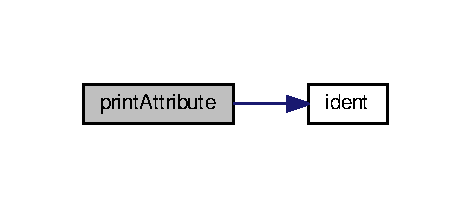
\includegraphics[width=226pt]{attributes_8c_aee295c33031c2ab941c9260654010db7_cgraph}
\end{center}
\end{figure}




Este é o diagrama das funções que utilizam esta função\+:\nopagebreak
\begin{figure}[H]
\begin{center}
\leavevmode
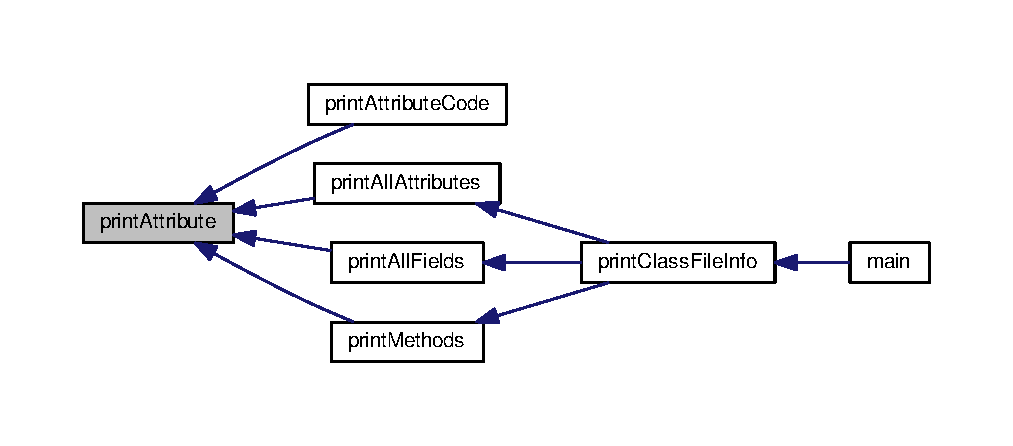
\includegraphics[width=350pt]{attributes_8c_aee295c33031c2ab941c9260654010db7_icgraph}
\end{center}
\end{figure}


\index{attributes.\+c@{attributes.\+c}!print\+Attribute\+Code@{print\+Attribute\+Code}}
\index{print\+Attribute\+Code@{print\+Attribute\+Code}!attributes.\+c@{attributes.\+c}}
\subsubsection[{\texorpdfstring{print\+Attribute\+Code(\+Java\+Class $\ast$jc, attribute\+\_\+info $\ast$entry, int identation\+Level)}{printAttributeCode(JavaClass *jc, attribute_info *entry, int identationLevel)}}]{\setlength{\rightskip}{0pt plus 5cm}void print\+Attribute\+Code (
\begin{DoxyParamCaption}
\item[{{\bf Java\+Class} $\ast$}]{jc, }
\item[{{\bf attribute\+\_\+info} $\ast$}]{entry, }
\item[{int}]{identation\+Level}
\end{DoxyParamCaption}
)}\hypertarget{attributes_8c_ae588cbde97553719c8b8612e8e42f4b4}{}\label{attributes_8c_ae588cbde97553719c8b8612e8e42f4b4}


Grafo de chamadas desta função\+:\nopagebreak
\begin{figure}[H]
\begin{center}
\leavevmode
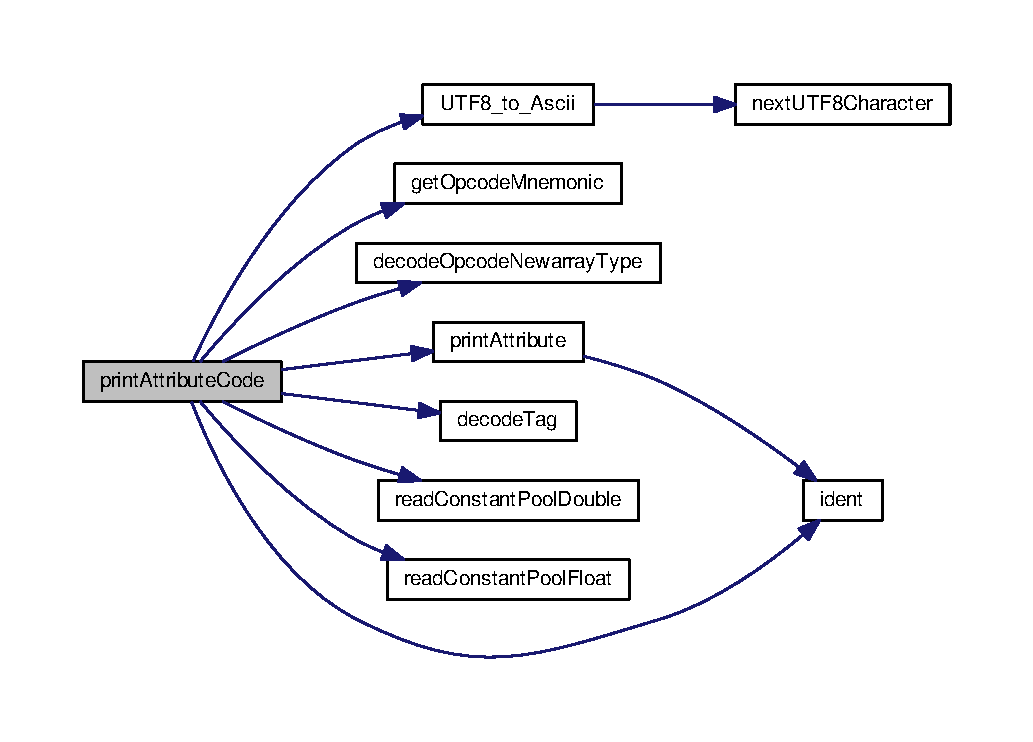
\includegraphics[width=350pt]{attributes_8c_ae588cbde97553719c8b8612e8e42f4b4_cgraph}
\end{center}
\end{figure}


\index{attributes.\+c@{attributes.\+c}!print\+Attribute\+Constant\+Value@{print\+Attribute\+Constant\+Value}}
\index{print\+Attribute\+Constant\+Value@{print\+Attribute\+Constant\+Value}!attributes.\+c@{attributes.\+c}}
\subsubsection[{\texorpdfstring{print\+Attribute\+Constant\+Value(\+Java\+Class $\ast$jc, attribute\+\_\+info $\ast$entry, int identation\+Level)}{printAttributeConstantValue(JavaClass *jc, attribute_info *entry, int identationLevel)}}]{\setlength{\rightskip}{0pt plus 5cm}void print\+Attribute\+Constant\+Value (
\begin{DoxyParamCaption}
\item[{{\bf Java\+Class} $\ast$}]{jc, }
\item[{{\bf attribute\+\_\+info} $\ast$}]{entry, }
\item[{int}]{identation\+Level}
\end{DoxyParamCaption}
)}\hypertarget{attributes_8c_a5abd76089f5e6794d1ecc98cea55f158}{}\label{attributes_8c_a5abd76089f5e6794d1ecc98cea55f158}


Grafo de chamadas desta função\+:\nopagebreak
\begin{figure}[H]
\begin{center}
\leavevmode
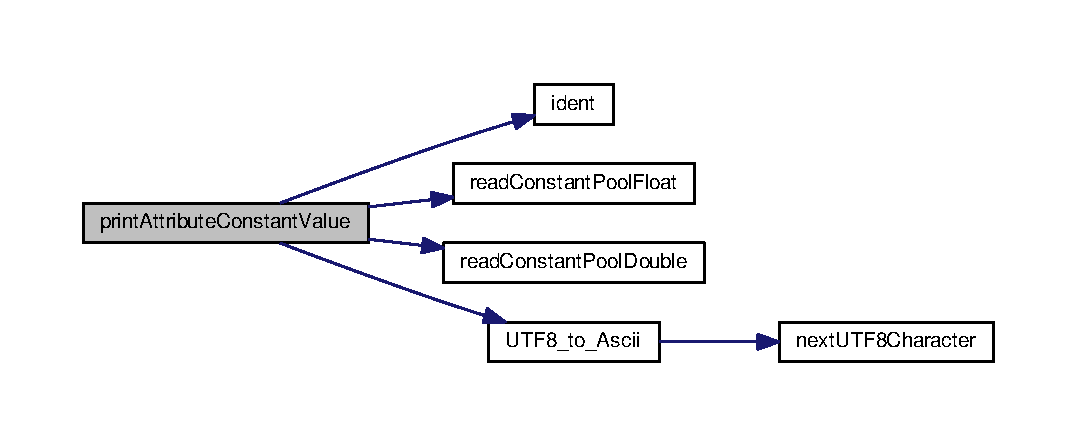
\includegraphics[width=350pt]{attributes_8c_a5abd76089f5e6794d1ecc98cea55f158_cgraph}
\end{center}
\end{figure}


\index{attributes.\+c@{attributes.\+c}!print\+Attribute\+Deprecated@{print\+Attribute\+Deprecated}}
\index{print\+Attribute\+Deprecated@{print\+Attribute\+Deprecated}!attributes.\+c@{attributes.\+c}}
\subsubsection[{\texorpdfstring{print\+Attribute\+Deprecated(\+Java\+Class $\ast$jc, attribute\+\_\+info $\ast$entry, int identation\+Level)}{printAttributeDeprecated(JavaClass *jc, attribute_info *entry, int identationLevel)}}]{\setlength{\rightskip}{0pt plus 5cm}void print\+Attribute\+Deprecated (
\begin{DoxyParamCaption}
\item[{{\bf Java\+Class} $\ast$}]{jc, }
\item[{{\bf attribute\+\_\+info} $\ast$}]{entry, }
\item[{int}]{identation\+Level}
\end{DoxyParamCaption}
)}\hypertarget{attributes_8c_ad80e46006ae1ca8e80f84735d331fc18}{}\label{attributes_8c_ad80e46006ae1ca8e80f84735d331fc18}


Grafo de chamadas desta função\+:\nopagebreak
\begin{figure}[H]
\begin{center}
\leavevmode
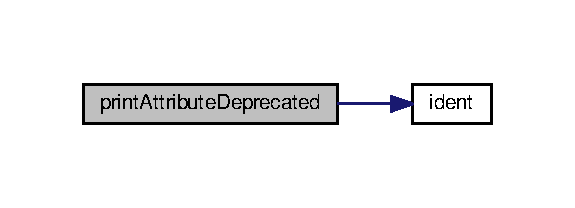
\includegraphics[width=276pt]{attributes_8c_ad80e46006ae1ca8e80f84735d331fc18_cgraph}
\end{center}
\end{figure}


\index{attributes.\+c@{attributes.\+c}!print\+Attribute\+Exceptions@{print\+Attribute\+Exceptions}}
\index{print\+Attribute\+Exceptions@{print\+Attribute\+Exceptions}!attributes.\+c@{attributes.\+c}}
\subsubsection[{\texorpdfstring{print\+Attribute\+Exceptions(\+Java\+Class $\ast$jc, attribute\+\_\+info $\ast$entry, int identation\+Level)}{printAttributeExceptions(JavaClass *jc, attribute_info *entry, int identationLevel)}}]{\setlength{\rightskip}{0pt plus 5cm}void print\+Attribute\+Exceptions (
\begin{DoxyParamCaption}
\item[{{\bf Java\+Class} $\ast$}]{jc, }
\item[{{\bf attribute\+\_\+info} $\ast$}]{entry, }
\item[{int}]{identation\+Level}
\end{DoxyParamCaption}
)}\hypertarget{attributes_8c_a1aeef532497a7cc1a3dee89d104bd725}{}\label{attributes_8c_a1aeef532497a7cc1a3dee89d104bd725}


Grafo de chamadas desta função\+:\nopagebreak
\begin{figure}[H]
\begin{center}
\leavevmode
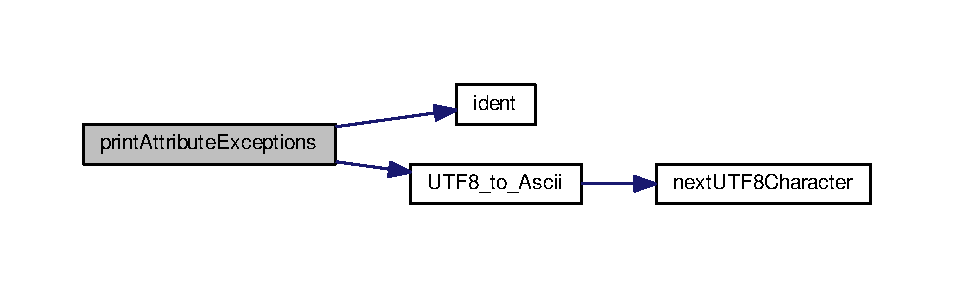
\includegraphics[width=350pt]{attributes_8c_a1aeef532497a7cc1a3dee89d104bd725_cgraph}
\end{center}
\end{figure}


\index{attributes.\+c@{attributes.\+c}!print\+Attribute\+Inner\+Classes@{print\+Attribute\+Inner\+Classes}}
\index{print\+Attribute\+Inner\+Classes@{print\+Attribute\+Inner\+Classes}!attributes.\+c@{attributes.\+c}}
\subsubsection[{\texorpdfstring{print\+Attribute\+Inner\+Classes(\+Java\+Class $\ast$jc, attribute\+\_\+info $\ast$entry, int identation\+Level)}{printAttributeInnerClasses(JavaClass *jc, attribute_info *entry, int identationLevel)}}]{\setlength{\rightskip}{0pt plus 5cm}void print\+Attribute\+Inner\+Classes (
\begin{DoxyParamCaption}
\item[{{\bf Java\+Class} $\ast$}]{jc, }
\item[{{\bf attribute\+\_\+info} $\ast$}]{entry, }
\item[{int}]{identation\+Level}
\end{DoxyParamCaption}
)}\hypertarget{attributes_8c_a6c90c1dd47892d19d581ef9fcac24698}{}\label{attributes_8c_a6c90c1dd47892d19d581ef9fcac24698}


Grafo de chamadas desta função\+:\nopagebreak
\begin{figure}[H]
\begin{center}
\leavevmode
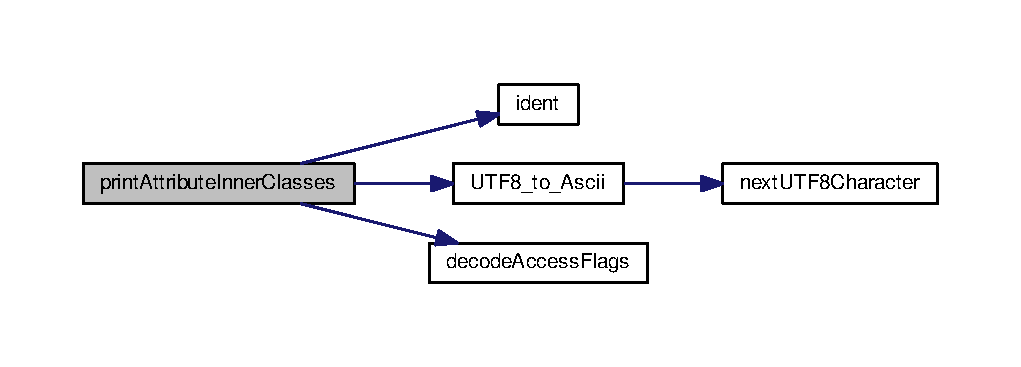
\includegraphics[width=350pt]{attributes_8c_a6c90c1dd47892d19d581ef9fcac24698_cgraph}
\end{center}
\end{figure}


\index{attributes.\+c@{attributes.\+c}!print\+Attribute\+Line\+Number\+Table@{print\+Attribute\+Line\+Number\+Table}}
\index{print\+Attribute\+Line\+Number\+Table@{print\+Attribute\+Line\+Number\+Table}!attributes.\+c@{attributes.\+c}}
\subsubsection[{\texorpdfstring{print\+Attribute\+Line\+Number\+Table(\+Java\+Class $\ast$jc, attribute\+\_\+info $\ast$entry, int identation\+Level)}{printAttributeLineNumberTable(JavaClass *jc, attribute_info *entry, int identationLevel)}}]{\setlength{\rightskip}{0pt plus 5cm}void print\+Attribute\+Line\+Number\+Table (
\begin{DoxyParamCaption}
\item[{{\bf Java\+Class} $\ast$}]{jc, }
\item[{{\bf attribute\+\_\+info} $\ast$}]{entry, }
\item[{int}]{identation\+Level}
\end{DoxyParamCaption}
)}\hypertarget{attributes_8c_a8c510d03555d15e558997e15e000c40f}{}\label{attributes_8c_a8c510d03555d15e558997e15e000c40f}


Grafo de chamadas desta função\+:\nopagebreak
\begin{figure}[H]
\begin{center}
\leavevmode
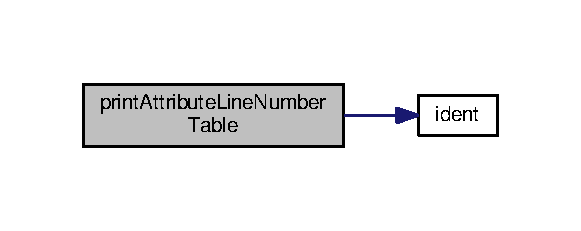
\includegraphics[width=279pt]{attributes_8c_a8c510d03555d15e558997e15e000c40f_cgraph}
\end{center}
\end{figure}


\index{attributes.\+c@{attributes.\+c}!print\+Attribute\+Source\+File@{print\+Attribute\+Source\+File}}
\index{print\+Attribute\+Source\+File@{print\+Attribute\+Source\+File}!attributes.\+c@{attributes.\+c}}
\subsubsection[{\texorpdfstring{print\+Attribute\+Source\+File(\+Java\+Class $\ast$jc, attribute\+\_\+info $\ast$entry, int identation\+Level)}{printAttributeSourceFile(JavaClass *jc, attribute_info *entry, int identationLevel)}}]{\setlength{\rightskip}{0pt plus 5cm}void print\+Attribute\+Source\+File (
\begin{DoxyParamCaption}
\item[{{\bf Java\+Class} $\ast$}]{jc, }
\item[{{\bf attribute\+\_\+info} $\ast$}]{entry, }
\item[{int}]{identation\+Level}
\end{DoxyParamCaption}
)}\hypertarget{attributes_8c_a7566e0f5a2ba5992f6e8f84a7b5d0b8b}{}\label{attributes_8c_a7566e0f5a2ba5992f6e8f84a7b5d0b8b}


Grafo de chamadas desta função\+:\nopagebreak
\begin{figure}[H]
\begin{center}
\leavevmode
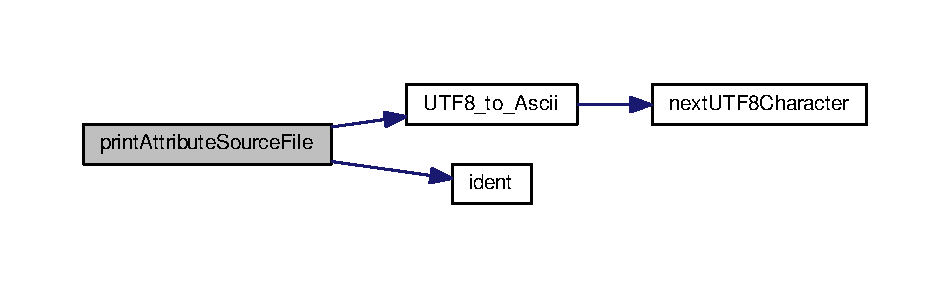
\includegraphics[width=350pt]{attributes_8c_a7566e0f5a2ba5992f6e8f84a7b5d0b8b_cgraph}
\end{center}
\end{figure}


\index{attributes.\+c@{attributes.\+c}!read\+Attribute@{read\+Attribute}}
\index{read\+Attribute@{read\+Attribute}!attributes.\+c@{attributes.\+c}}
\subsubsection[{\texorpdfstring{read\+Attribute(\+Java\+Class $\ast$jc, attribute\+\_\+info $\ast$entry)}{readAttribute(JavaClass *jc, attribute_info *entry)}}]{\setlength{\rightskip}{0pt plus 5cm}char read\+Attribute (
\begin{DoxyParamCaption}
\item[{{\bf Java\+Class} $\ast$}]{jc, }
\item[{{\bf attribute\+\_\+info} $\ast$}]{entry}
\end{DoxyParamCaption}
)}\hypertarget{attributes_8c_a0aab7731ade76c16c2ff8b3bef1111d1}{}\label{attributes_8c_a0aab7731ade76c16c2ff8b3bef1111d1}


Grafo de chamadas desta função\+:\nopagebreak
\begin{figure}[H]
\begin{center}
\leavevmode
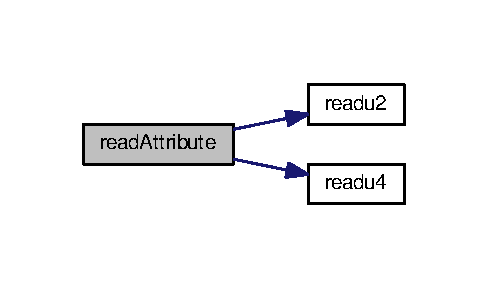
\includegraphics[width=234pt]{attributes_8c_a0aab7731ade76c16c2ff8b3bef1111d1_cgraph}
\end{center}
\end{figure}




Este é o diagrama das funções que utilizam esta função\+:\nopagebreak
\begin{figure}[H]
\begin{center}
\leavevmode
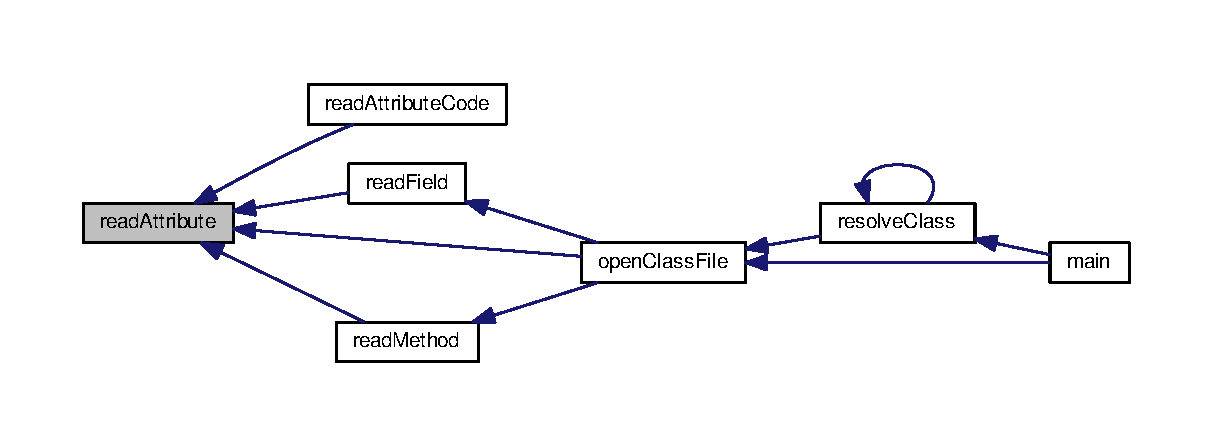
\includegraphics[width=350pt]{attributes_8c_a0aab7731ade76c16c2ff8b3bef1111d1_icgraph}
\end{center}
\end{figure}


\index{attributes.\+c@{attributes.\+c}!read\+Attribute\+Code@{read\+Attribute\+Code}}
\index{read\+Attribute\+Code@{read\+Attribute\+Code}!attributes.\+c@{attributes.\+c}}
\subsubsection[{\texorpdfstring{read\+Attribute\+Code(\+Java\+Class $\ast$jc, attribute\+\_\+info $\ast$entry)}{readAttributeCode(JavaClass *jc, attribute_info *entry)}}]{\setlength{\rightskip}{0pt plus 5cm}uint8\+\_\+t read\+Attribute\+Code (
\begin{DoxyParamCaption}
\item[{{\bf Java\+Class} $\ast$}]{jc, }
\item[{{\bf attribute\+\_\+info} $\ast$}]{entry}
\end{DoxyParamCaption}
)}\hypertarget{attributes_8c_af3a1b04442990e1699afc5b2592c4c93}{}\label{attributes_8c_af3a1b04442990e1699afc5b2592c4c93}


Grafo de chamadas desta função\+:\nopagebreak
\begin{figure}[H]
\begin{center}
\leavevmode
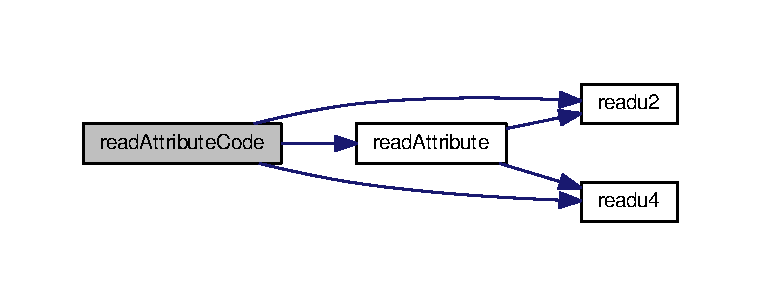
\includegraphics[width=350pt]{attributes_8c_af3a1b04442990e1699afc5b2592c4c93_cgraph}
\end{center}
\end{figure}


\index{attributes.\+c@{attributes.\+c}!read\+Attribute\+Constant\+Value@{read\+Attribute\+Constant\+Value}}
\index{read\+Attribute\+Constant\+Value@{read\+Attribute\+Constant\+Value}!attributes.\+c@{attributes.\+c}}
\subsubsection[{\texorpdfstring{read\+Attribute\+Constant\+Value(\+Java\+Class $\ast$jc, attribute\+\_\+info $\ast$entry)}{readAttributeConstantValue(JavaClass *jc, attribute_info *entry)}}]{\setlength{\rightskip}{0pt plus 5cm}uint8\+\_\+t read\+Attribute\+Constant\+Value (
\begin{DoxyParamCaption}
\item[{{\bf Java\+Class} $\ast$}]{jc, }
\item[{{\bf attribute\+\_\+info} $\ast$}]{entry}
\end{DoxyParamCaption}
)}\hypertarget{attributes_8c_ac07fa201160b522b15c7353b4ff2ed44}{}\label{attributes_8c_ac07fa201160b522b15c7353b4ff2ed44}


Grafo de chamadas desta função\+:\nopagebreak
\begin{figure}[H]
\begin{center}
\leavevmode
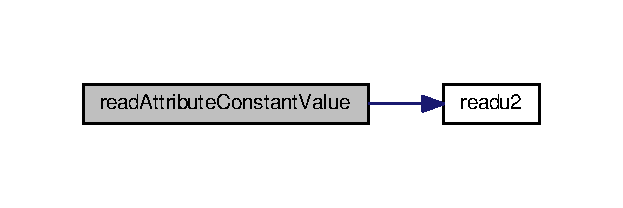
\includegraphics[width=299pt]{attributes_8c_ac07fa201160b522b15c7353b4ff2ed44_cgraph}
\end{center}
\end{figure}


\index{attributes.\+c@{attributes.\+c}!read\+Attribute\+Deprecated@{read\+Attribute\+Deprecated}}
\index{read\+Attribute\+Deprecated@{read\+Attribute\+Deprecated}!attributes.\+c@{attributes.\+c}}
\subsubsection[{\texorpdfstring{read\+Attribute\+Deprecated(\+Java\+Class $\ast$jc, attribute\+\_\+info $\ast$entry)}{readAttributeDeprecated(JavaClass *jc, attribute_info *entry)}}]{\setlength{\rightskip}{0pt plus 5cm}uint8\+\_\+t read\+Attribute\+Deprecated (
\begin{DoxyParamCaption}
\item[{{\bf Java\+Class} $\ast$}]{jc, }
\item[{{\bf attribute\+\_\+info} $\ast$}]{entry}
\end{DoxyParamCaption}
)}\hypertarget{attributes_8c_a5e568e134ff6fb82b263565076da0432}{}\label{attributes_8c_a5e568e134ff6fb82b263565076da0432}
\index{attributes.\+c@{attributes.\+c}!read\+Attribute\+Exceptions@{read\+Attribute\+Exceptions}}
\index{read\+Attribute\+Exceptions@{read\+Attribute\+Exceptions}!attributes.\+c@{attributes.\+c}}
\subsubsection[{\texorpdfstring{read\+Attribute\+Exceptions(\+Java\+Class $\ast$jc, attribute\+\_\+info $\ast$entry)}{readAttributeExceptions(JavaClass *jc, attribute_info *entry)}}]{\setlength{\rightskip}{0pt plus 5cm}uint8\+\_\+t read\+Attribute\+Exceptions (
\begin{DoxyParamCaption}
\item[{{\bf Java\+Class} $\ast$}]{jc, }
\item[{{\bf attribute\+\_\+info} $\ast$}]{entry}
\end{DoxyParamCaption}
)}\hypertarget{attributes_8c_a1aabfbdd22c8a11214ee3db33624b734}{}\label{attributes_8c_a1aabfbdd22c8a11214ee3db33624b734}


Grafo de chamadas desta função\+:\nopagebreak
\begin{figure}[H]
\begin{center}
\leavevmode
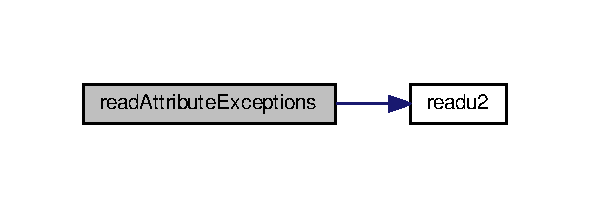
\includegraphics[width=283pt]{attributes_8c_a1aabfbdd22c8a11214ee3db33624b734_cgraph}
\end{center}
\end{figure}


\index{attributes.\+c@{attributes.\+c}!read\+Attribute\+Inner\+Classes@{read\+Attribute\+Inner\+Classes}}
\index{read\+Attribute\+Inner\+Classes@{read\+Attribute\+Inner\+Classes}!attributes.\+c@{attributes.\+c}}
\subsubsection[{\texorpdfstring{read\+Attribute\+Inner\+Classes(\+Java\+Class $\ast$jc, attribute\+\_\+info $\ast$entry)}{readAttributeInnerClasses(JavaClass *jc, attribute_info *entry)}}]{\setlength{\rightskip}{0pt plus 5cm}uint8\+\_\+t read\+Attribute\+Inner\+Classes (
\begin{DoxyParamCaption}
\item[{{\bf Java\+Class} $\ast$}]{jc, }
\item[{{\bf attribute\+\_\+info} $\ast$}]{entry}
\end{DoxyParamCaption}
)}\hypertarget{attributes_8c_a7af979b9e909d50393f578f9cf230fae}{}\label{attributes_8c_a7af979b9e909d50393f578f9cf230fae}


Grafo de chamadas desta função\+:\nopagebreak
\begin{figure}[H]
\begin{center}
\leavevmode
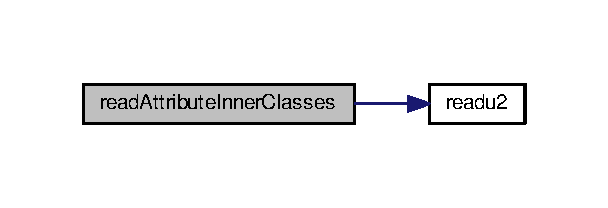
\includegraphics[width=292pt]{attributes_8c_a7af979b9e909d50393f578f9cf230fae_cgraph}
\end{center}
\end{figure}


\index{attributes.\+c@{attributes.\+c}!read\+Attribute\+Line\+Number\+Table@{read\+Attribute\+Line\+Number\+Table}}
\index{read\+Attribute\+Line\+Number\+Table@{read\+Attribute\+Line\+Number\+Table}!attributes.\+c@{attributes.\+c}}
\subsubsection[{\texorpdfstring{read\+Attribute\+Line\+Number\+Table(\+Java\+Class $\ast$jc, attribute\+\_\+info $\ast$entry)}{readAttributeLineNumberTable(JavaClass *jc, attribute_info *entry)}}]{\setlength{\rightskip}{0pt plus 5cm}uint8\+\_\+t read\+Attribute\+Line\+Number\+Table (
\begin{DoxyParamCaption}
\item[{{\bf Java\+Class} $\ast$}]{jc, }
\item[{{\bf attribute\+\_\+info} $\ast$}]{entry}
\end{DoxyParamCaption}
)}\hypertarget{attributes_8c_a837af1196cf968ff688539be299648d5}{}\label{attributes_8c_a837af1196cf968ff688539be299648d5}


Grafo de chamadas desta função\+:\nopagebreak
\begin{figure}[H]
\begin{center}
\leavevmode
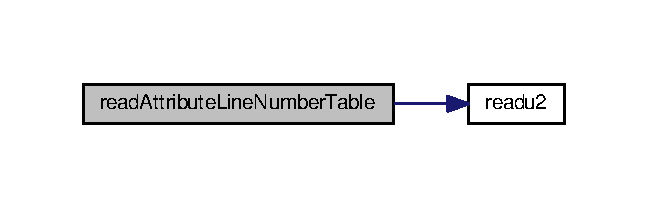
\includegraphics[width=311pt]{attributes_8c_a837af1196cf968ff688539be299648d5_cgraph}
\end{center}
\end{figure}


\index{attributes.\+c@{attributes.\+c}!read\+Attribute\+Source\+File@{read\+Attribute\+Source\+File}}
\index{read\+Attribute\+Source\+File@{read\+Attribute\+Source\+File}!attributes.\+c@{attributes.\+c}}
\subsubsection[{\texorpdfstring{read\+Attribute\+Source\+File(\+Java\+Class $\ast$jc, attribute\+\_\+info $\ast$entry)}{readAttributeSourceFile(JavaClass *jc, attribute_info *entry)}}]{\setlength{\rightskip}{0pt plus 5cm}uint8\+\_\+t read\+Attribute\+Source\+File (
\begin{DoxyParamCaption}
\item[{{\bf Java\+Class} $\ast$}]{jc, }
\item[{{\bf attribute\+\_\+info} $\ast$}]{entry}
\end{DoxyParamCaption}
)}\hypertarget{attributes_8c_a43bfb8cf040e623ccae73943a943a7f8}{}\label{attributes_8c_a43bfb8cf040e623ccae73943a943a7f8}


Grafo de chamadas desta função\+:\nopagebreak
\begin{figure}[H]
\begin{center}
\leavevmode
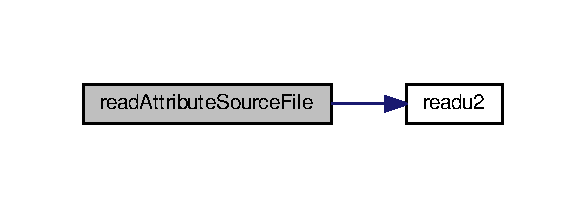
\includegraphics[width=281pt]{attributes_8c_a43bfb8cf040e623ccae73943a943a7f8_cgraph}
\end{center}
\end{figure}



\hypertarget{attributes_8h}{}\section{Referência ao ficheiro src/attributes.h}
\label{attributes_8h}\index{src/attributes.\+h@{src/attributes.\+h}}
{\ttfamily \#include $<$stdint.\+h$>$}\\*
{\ttfamily \#include \char`\"{}javaclass.\+h\char`\"{}}\\*
Diagrama de dependências de inclusão para attributes.\+h\+:\nopagebreak
\begin{figure}[H]
\begin{center}
\leavevmode
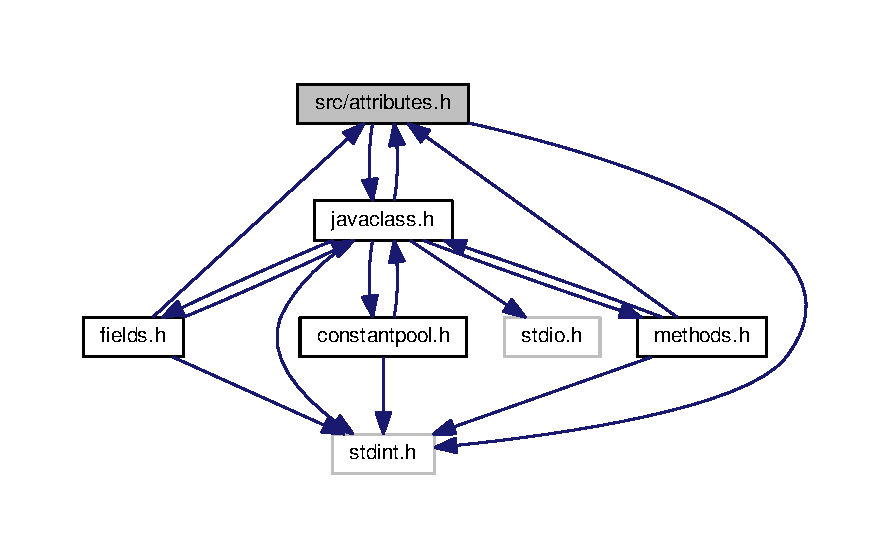
\includegraphics[width=350pt]{attributes_8h__incl}
\end{center}
\end{figure}
Este grafo mostra quais são os ficheiros que incluem directamente ou indirectamente este ficheiro\+:\nopagebreak
\begin{figure}[H]
\begin{center}
\leavevmode
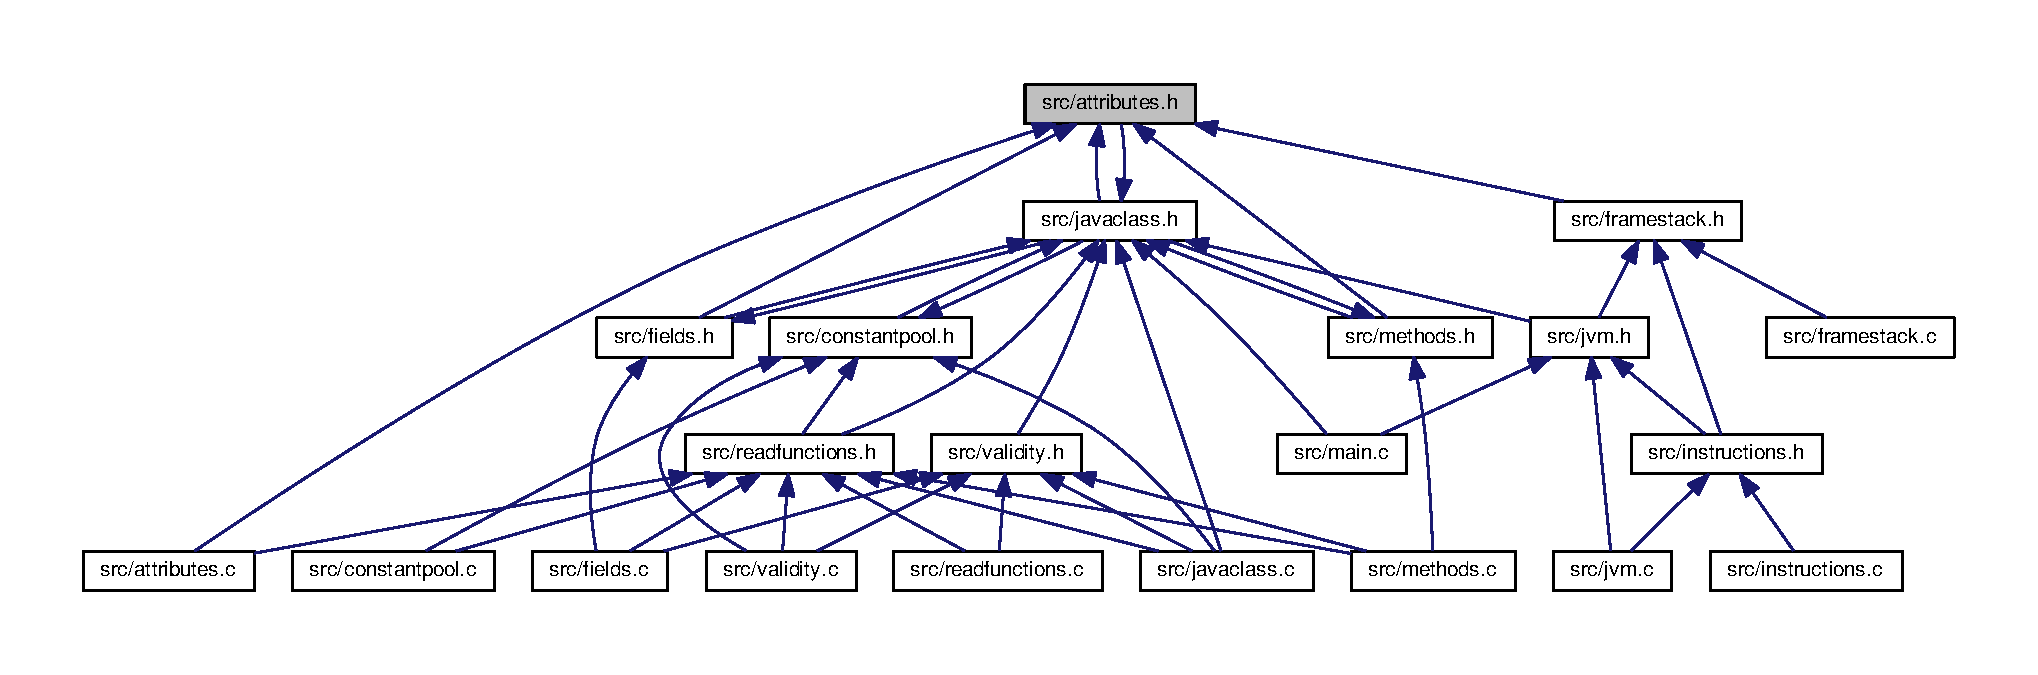
\includegraphics[width=350pt]{attributes_8h__dep__incl}
\end{center}
\end{figure}
\subsection*{Estruturas de Dados}
\begin{DoxyCompactItemize}
\item 
struct \hyperlink{structattribute__info}{attribute\+\_\+info}
\item 
struct \hyperlink{structatt__SourceFile__info}{att\+\_\+\+Source\+File\+\_\+info}
\item 
struct \hyperlink{structatt__ConstantValue__info}{att\+\_\+\+Constant\+Value\+\_\+info}
\item 
struct \hyperlink{structInnerClassInfo}{Inner\+Class\+Info}
\item 
struct \hyperlink{structatt__InnerClasses__info}{att\+\_\+\+Inner\+Classes\+\_\+info}
\item 
struct \hyperlink{structLineNumberTableEntry}{Line\+Number\+Table\+Entry}
\item 
struct \hyperlink{structatt__LineNumberTable__info}{att\+\_\+\+Line\+Number\+Table\+\_\+info}
\item 
struct \hyperlink{structExceptionTableEntry}{Exception\+Table\+Entry}
\item 
struct \hyperlink{structatt__Code__info}{att\+\_\+\+Code\+\_\+info}
\item 
struct \hyperlink{structatt__Exceptions__info}{att\+\_\+\+Exceptions\+\_\+info}
\end{DoxyCompactItemize}
\subsection*{Definições de tipos}
\begin{DoxyCompactItemize}
\item 
typedef struct \hyperlink{structattribute__info}{attribute\+\_\+info} \hyperlink{attributes_8h_a7b1e7b81c7ca3b550a1973f2d8672950}{attribute\+\_\+info}
\end{DoxyCompactItemize}
\subsection*{Enumerações}
\begin{DoxyCompactItemize}
\item 
enum \hyperlink{attributes_8h_a349a9cde14be8097df865ba0469c0ab2}{Attribute\+Type} \{ \\*
\hyperlink{attributes_8h_a349a9cde14be8097df865ba0469c0ab2a84368a0bd5b017d16829889f6fc586b8}{A\+T\+T\+R\+\_\+\+Unknown} = 0, 
\hyperlink{attributes_8h_a349a9cde14be8097df865ba0469c0ab2a48c63d4adab3bf466ab67ee39155bf89}{A\+T\+T\+R\+\_\+\+Constant\+Value}, 
\hyperlink{attributes_8h_a349a9cde14be8097df865ba0469c0ab2a82e29efd5d3c5c77fabf5997ff6da5c2}{A\+T\+T\+R\+\_\+\+Source\+File}, 
\hyperlink{attributes_8h_a349a9cde14be8097df865ba0469c0ab2aa1e111a1adfd4ce3ae583df564a90e09}{A\+T\+T\+R\+\_\+\+Inner\+Classes}, 
\\*
\hyperlink{attributes_8h_a349a9cde14be8097df865ba0469c0ab2a6b8593cf0987a37a80a03e197299597e}{A\+T\+T\+R\+\_\+\+Code}, 
\hyperlink{attributes_8h_a349a9cde14be8097df865ba0469c0ab2a3a2254220839b1156d1eb800f1035e66}{A\+T\+T\+R\+\_\+\+Line\+Number\+Table}, 
\hyperlink{attributes_8h_a349a9cde14be8097df865ba0469c0ab2aa75264de718d1ea76625fb8236133d61}{A\+T\+T\+R\+\_\+\+Exceptions}, 
\hyperlink{attributes_8h_a349a9cde14be8097df865ba0469c0ab2aa8687d6c4b71efe81907687ed84d103a}{A\+T\+T\+R\+\_\+\+Deprecated}
 \}
\end{DoxyCompactItemize}
\subsection*{Funções}
\begin{DoxyCompactItemize}
\item 
char \hyperlink{attributes_8h_a0aab7731ade76c16c2ff8b3bef1111d1}{read\+Attribute} (\hyperlink{structJavaClass}{Java\+Class} $\ast$jc, \hyperlink{structattribute__info}{attribute\+\_\+info} $\ast$entry)
\item 
void \hyperlink{attributes_8h_a136bdfadd787ebd62f1c721f99270cc9}{free\+Attribute\+Info} (\hyperlink{structattribute__info}{attribute\+\_\+info} $\ast$entry)
\item 
void \hyperlink{attributes_8h_aee295c33031c2ab941c9260654010db7}{print\+Attribute} (\hyperlink{structJavaClass}{Java\+Class} $\ast$jc, \hyperlink{structattribute__info}{attribute\+\_\+info} $\ast$entry, int identation\+Level)
\item 
void \hyperlink{attributes_8h_ae04e26b66957c879139f8a82e463674a}{print\+All\+Attributes} (\hyperlink{structJavaClass}{Java\+Class} $\ast$jc)
\item 
\hyperlink{structattribute__info}{attribute\+\_\+info} $\ast$ \hyperlink{attributes_8h_ae3ce1b33741046741c90a6f5592911a5}{get\+Attribute\+By\+Type} (\hyperlink{structattribute__info}{attribute\+\_\+info} $\ast$attributes, uint16\+\_\+t attributes\+\_\+length, enum \hyperlink{attributes_8h_a349a9cde14be8097df865ba0469c0ab2}{Attribute\+Type} type)
\end{DoxyCompactItemize}


\subsection{Documentação dos tipos}
\index{attributes.\+h@{attributes.\+h}!attribute\+\_\+info@{attribute\+\_\+info}}
\index{attribute\+\_\+info@{attribute\+\_\+info}!attributes.\+h@{attributes.\+h}}
\subsubsection[{\texorpdfstring{attribute\+\_\+info}{attribute_info}}]{\setlength{\rightskip}{0pt plus 5cm}typedef struct {\bf attribute\+\_\+info} {\bf attribute\+\_\+info}}\hypertarget{attributes_8h_a7b1e7b81c7ca3b550a1973f2d8672950}{}\label{attributes_8h_a7b1e7b81c7ca3b550a1973f2d8672950}


\subsection{Documentação dos valores da enumeração}
\index{attributes.\+h@{attributes.\+h}!Attribute\+Type@{Attribute\+Type}}
\index{Attribute\+Type@{Attribute\+Type}!attributes.\+h@{attributes.\+h}}
\subsubsection[{\texorpdfstring{Attribute\+Type}{AttributeType}}]{\setlength{\rightskip}{0pt plus 5cm}enum {\bf Attribute\+Type}}\hypertarget{attributes_8h_a349a9cde14be8097df865ba0469c0ab2}{}\label{attributes_8h_a349a9cde14be8097df865ba0469c0ab2}
\begin{Desc}
\item[Valores de enumerações]\par
\begin{description}
\index{A\+T\+T\+R\+\_\+\+Unknown@{A\+T\+T\+R\+\_\+\+Unknown}!attributes.\+h@{attributes.\+h}}\index{attributes.\+h@{attributes.\+h}!A\+T\+T\+R\+\_\+\+Unknown@{A\+T\+T\+R\+\_\+\+Unknown}}\item[{\em 
A\+T\+T\+R\+\_\+\+Unknown\hypertarget{attributes_8h_a349a9cde14be8097df865ba0469c0ab2a84368a0bd5b017d16829889f6fc586b8}{}\label{attributes_8h_a349a9cde14be8097df865ba0469c0ab2a84368a0bd5b017d16829889f6fc586b8}
}]\index{A\+T\+T\+R\+\_\+\+Constant\+Value@{A\+T\+T\+R\+\_\+\+Constant\+Value}!attributes.\+h@{attributes.\+h}}\index{attributes.\+h@{attributes.\+h}!A\+T\+T\+R\+\_\+\+Constant\+Value@{A\+T\+T\+R\+\_\+\+Constant\+Value}}\item[{\em 
A\+T\+T\+R\+\_\+\+Constant\+Value\hypertarget{attributes_8h_a349a9cde14be8097df865ba0469c0ab2a48c63d4adab3bf466ab67ee39155bf89}{}\label{attributes_8h_a349a9cde14be8097df865ba0469c0ab2a48c63d4adab3bf466ab67ee39155bf89}
}]\index{A\+T\+T\+R\+\_\+\+Source\+File@{A\+T\+T\+R\+\_\+\+Source\+File}!attributes.\+h@{attributes.\+h}}\index{attributes.\+h@{attributes.\+h}!A\+T\+T\+R\+\_\+\+Source\+File@{A\+T\+T\+R\+\_\+\+Source\+File}}\item[{\em 
A\+T\+T\+R\+\_\+\+Source\+File\hypertarget{attributes_8h_a349a9cde14be8097df865ba0469c0ab2a82e29efd5d3c5c77fabf5997ff6da5c2}{}\label{attributes_8h_a349a9cde14be8097df865ba0469c0ab2a82e29efd5d3c5c77fabf5997ff6da5c2}
}]\index{A\+T\+T\+R\+\_\+\+Inner\+Classes@{A\+T\+T\+R\+\_\+\+Inner\+Classes}!attributes.\+h@{attributes.\+h}}\index{attributes.\+h@{attributes.\+h}!A\+T\+T\+R\+\_\+\+Inner\+Classes@{A\+T\+T\+R\+\_\+\+Inner\+Classes}}\item[{\em 
A\+T\+T\+R\+\_\+\+Inner\+Classes\hypertarget{attributes_8h_a349a9cde14be8097df865ba0469c0ab2aa1e111a1adfd4ce3ae583df564a90e09}{}\label{attributes_8h_a349a9cde14be8097df865ba0469c0ab2aa1e111a1adfd4ce3ae583df564a90e09}
}]\index{A\+T\+T\+R\+\_\+\+Code@{A\+T\+T\+R\+\_\+\+Code}!attributes.\+h@{attributes.\+h}}\index{attributes.\+h@{attributes.\+h}!A\+T\+T\+R\+\_\+\+Code@{A\+T\+T\+R\+\_\+\+Code}}\item[{\em 
A\+T\+T\+R\+\_\+\+Code\hypertarget{attributes_8h_a349a9cde14be8097df865ba0469c0ab2a6b8593cf0987a37a80a03e197299597e}{}\label{attributes_8h_a349a9cde14be8097df865ba0469c0ab2a6b8593cf0987a37a80a03e197299597e}
}]\index{A\+T\+T\+R\+\_\+\+Line\+Number\+Table@{A\+T\+T\+R\+\_\+\+Line\+Number\+Table}!attributes.\+h@{attributes.\+h}}\index{attributes.\+h@{attributes.\+h}!A\+T\+T\+R\+\_\+\+Line\+Number\+Table@{A\+T\+T\+R\+\_\+\+Line\+Number\+Table}}\item[{\em 
A\+T\+T\+R\+\_\+\+Line\+Number\+Table\hypertarget{attributes_8h_a349a9cde14be8097df865ba0469c0ab2a3a2254220839b1156d1eb800f1035e66}{}\label{attributes_8h_a349a9cde14be8097df865ba0469c0ab2a3a2254220839b1156d1eb800f1035e66}
}]\index{A\+T\+T\+R\+\_\+\+Exceptions@{A\+T\+T\+R\+\_\+\+Exceptions}!attributes.\+h@{attributes.\+h}}\index{attributes.\+h@{attributes.\+h}!A\+T\+T\+R\+\_\+\+Exceptions@{A\+T\+T\+R\+\_\+\+Exceptions}}\item[{\em 
A\+T\+T\+R\+\_\+\+Exceptions\hypertarget{attributes_8h_a349a9cde14be8097df865ba0469c0ab2aa75264de718d1ea76625fb8236133d61}{}\label{attributes_8h_a349a9cde14be8097df865ba0469c0ab2aa75264de718d1ea76625fb8236133d61}
}]\index{A\+T\+T\+R\+\_\+\+Deprecated@{A\+T\+T\+R\+\_\+\+Deprecated}!attributes.\+h@{attributes.\+h}}\index{attributes.\+h@{attributes.\+h}!A\+T\+T\+R\+\_\+\+Deprecated@{A\+T\+T\+R\+\_\+\+Deprecated}}\item[{\em 
A\+T\+T\+R\+\_\+\+Deprecated\hypertarget{attributes_8h_a349a9cde14be8097df865ba0469c0ab2aa8687d6c4b71efe81907687ed84d103a}{}\label{attributes_8h_a349a9cde14be8097df865ba0469c0ab2aa8687d6c4b71efe81907687ed84d103a}
}]\end{description}
\end{Desc}


\subsection{Documentação das funções}
\index{attributes.\+h@{attributes.\+h}!free\+Attribute\+Info@{free\+Attribute\+Info}}
\index{free\+Attribute\+Info@{free\+Attribute\+Info}!attributes.\+h@{attributes.\+h}}
\subsubsection[{\texorpdfstring{free\+Attribute\+Info(attribute\+\_\+info $\ast$entry)}{freeAttributeInfo(attribute_info *entry)}}]{\setlength{\rightskip}{0pt plus 5cm}void free\+Attribute\+Info (
\begin{DoxyParamCaption}
\item[{{\bf attribute\+\_\+info} $\ast$}]{entry}
\end{DoxyParamCaption}
)}\hypertarget{attributes_8h_a136bdfadd787ebd62f1c721f99270cc9}{}\label{attributes_8h_a136bdfadd787ebd62f1c721f99270cc9}


Este é o diagrama das funções que utilizam esta função\+:\nopagebreak
\begin{figure}[H]
\begin{center}
\leavevmode
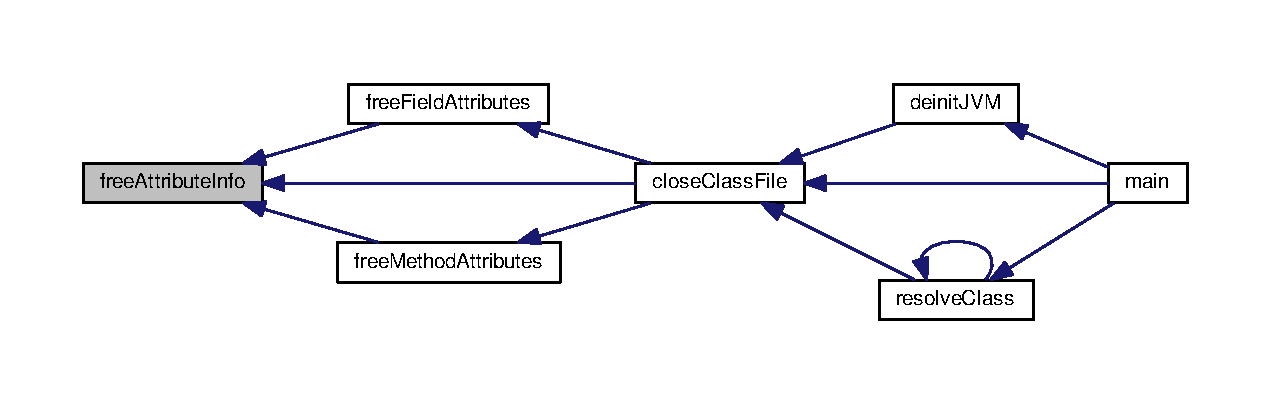
\includegraphics[width=350pt]{attributes_8h_a136bdfadd787ebd62f1c721f99270cc9_icgraph}
\end{center}
\end{figure}


\index{attributes.\+h@{attributes.\+h}!get\+Attribute\+By\+Type@{get\+Attribute\+By\+Type}}
\index{get\+Attribute\+By\+Type@{get\+Attribute\+By\+Type}!attributes.\+h@{attributes.\+h}}
\subsubsection[{\texorpdfstring{get\+Attribute\+By\+Type(attribute\+\_\+info $\ast$attributes, uint16\+\_\+t attributes\+\_\+length, enum Attribute\+Type type)}{getAttributeByType(attribute_info *attributes, uint16_t attributes_length, enum AttributeType type)}}]{\setlength{\rightskip}{0pt plus 5cm}{\bf attribute\+\_\+info}$\ast$ get\+Attribute\+By\+Type (
\begin{DoxyParamCaption}
\item[{{\bf attribute\+\_\+info} $\ast$}]{attributes, }
\item[{uint16\+\_\+t}]{attributes\+\_\+length, }
\item[{enum {\bf Attribute\+Type}}]{type}
\end{DoxyParamCaption}
)}\hypertarget{attributes_8h_ae3ce1b33741046741c90a6f5592911a5}{}\label{attributes_8h_ae3ce1b33741046741c90a6f5592911a5}


Este é o diagrama das funções que utilizam esta função\+:\nopagebreak
\begin{figure}[H]
\begin{center}
\leavevmode
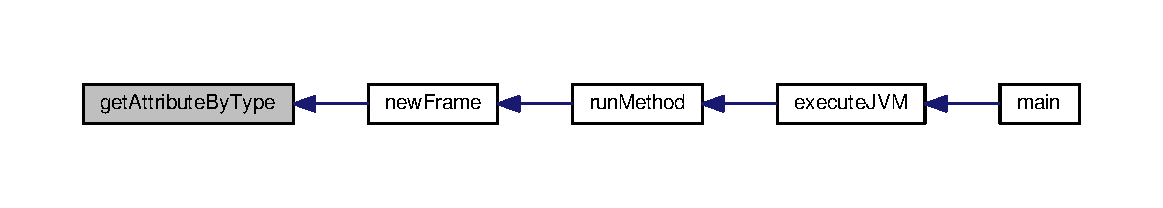
\includegraphics[width=350pt]{attributes_8h_ae3ce1b33741046741c90a6f5592911a5_icgraph}
\end{center}
\end{figure}


\index{attributes.\+h@{attributes.\+h}!print\+All\+Attributes@{print\+All\+Attributes}}
\index{print\+All\+Attributes@{print\+All\+Attributes}!attributes.\+h@{attributes.\+h}}
\subsubsection[{\texorpdfstring{print\+All\+Attributes(\+Java\+Class $\ast$jc)}{printAllAttributes(JavaClass *jc)}}]{\setlength{\rightskip}{0pt plus 5cm}void print\+All\+Attributes (
\begin{DoxyParamCaption}
\item[{{\bf Java\+Class} $\ast$}]{jc}
\end{DoxyParamCaption}
)}\hypertarget{attributes_8h_ae04e26b66957c879139f8a82e463674a}{}\label{attributes_8h_ae04e26b66957c879139f8a82e463674a}


Grafo de chamadas desta função\+:\nopagebreak
\begin{figure}[H]
\begin{center}
\leavevmode
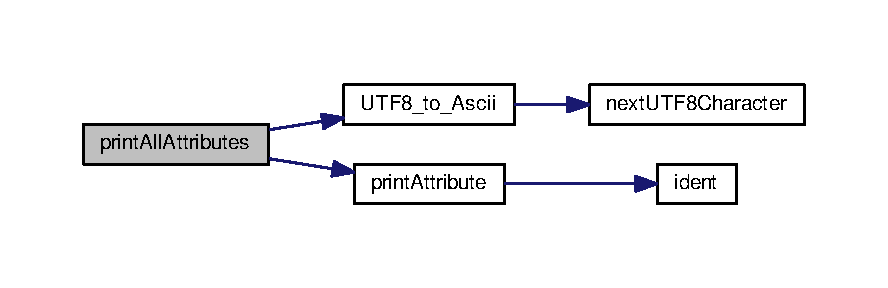
\includegraphics[width=350pt]{attributes_8h_ae04e26b66957c879139f8a82e463674a_cgraph}
\end{center}
\end{figure}




Este é o diagrama das funções que utilizam esta função\+:\nopagebreak
\begin{figure}[H]
\begin{center}
\leavevmode
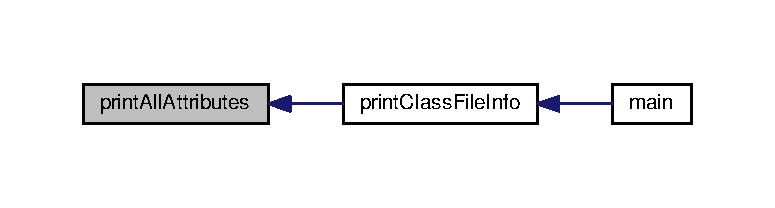
\includegraphics[width=350pt]{attributes_8h_ae04e26b66957c879139f8a82e463674a_icgraph}
\end{center}
\end{figure}


\index{attributes.\+h@{attributes.\+h}!print\+Attribute@{print\+Attribute}}
\index{print\+Attribute@{print\+Attribute}!attributes.\+h@{attributes.\+h}}
\subsubsection[{\texorpdfstring{print\+Attribute(\+Java\+Class $\ast$jc, attribute\+\_\+info $\ast$entry, int identation\+Level)}{printAttribute(JavaClass *jc, attribute_info *entry, int identationLevel)}}]{\setlength{\rightskip}{0pt plus 5cm}void print\+Attribute (
\begin{DoxyParamCaption}
\item[{{\bf Java\+Class} $\ast$}]{jc, }
\item[{{\bf attribute\+\_\+info} $\ast$}]{entry, }
\item[{int}]{identation\+Level}
\end{DoxyParamCaption}
)}\hypertarget{attributes_8h_aee295c33031c2ab941c9260654010db7}{}\label{attributes_8h_aee295c33031c2ab941c9260654010db7}


Grafo de chamadas desta função\+:\nopagebreak
\begin{figure}[H]
\begin{center}
\leavevmode
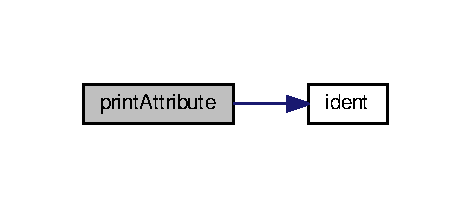
\includegraphics[width=226pt]{attributes_8h_aee295c33031c2ab941c9260654010db7_cgraph}
\end{center}
\end{figure}




Este é o diagrama das funções que utilizam esta função\+:\nopagebreak
\begin{figure}[H]
\begin{center}
\leavevmode
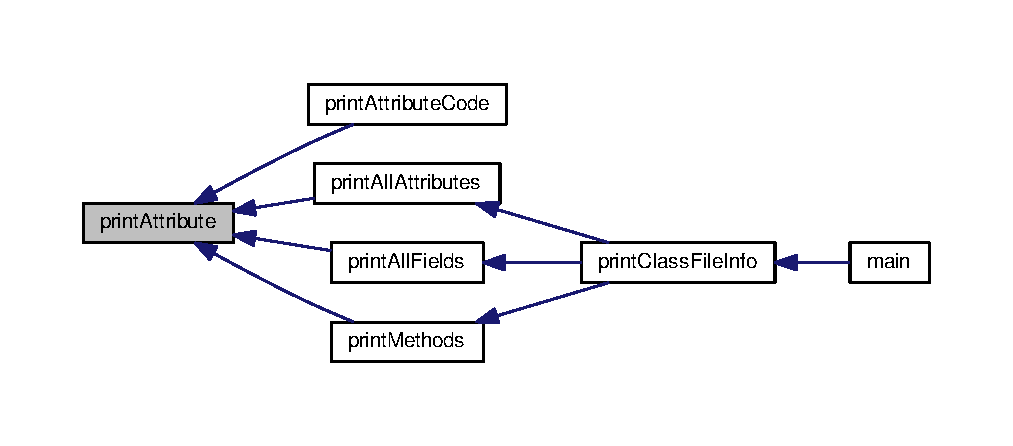
\includegraphics[width=350pt]{attributes_8h_aee295c33031c2ab941c9260654010db7_icgraph}
\end{center}
\end{figure}


\index{attributes.\+h@{attributes.\+h}!read\+Attribute@{read\+Attribute}}
\index{read\+Attribute@{read\+Attribute}!attributes.\+h@{attributes.\+h}}
\subsubsection[{\texorpdfstring{read\+Attribute(\+Java\+Class $\ast$jc, attribute\+\_\+info $\ast$entry)}{readAttribute(JavaClass *jc, attribute_info *entry)}}]{\setlength{\rightskip}{0pt plus 5cm}char read\+Attribute (
\begin{DoxyParamCaption}
\item[{{\bf Java\+Class} $\ast$}]{jc, }
\item[{{\bf attribute\+\_\+info} $\ast$}]{entry}
\end{DoxyParamCaption}
)}\hypertarget{attributes_8h_a0aab7731ade76c16c2ff8b3bef1111d1}{}\label{attributes_8h_a0aab7731ade76c16c2ff8b3bef1111d1}


Grafo de chamadas desta função\+:\nopagebreak
\begin{figure}[H]
\begin{center}
\leavevmode
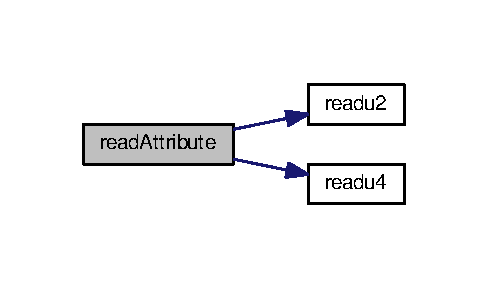
\includegraphics[width=234pt]{attributes_8h_a0aab7731ade76c16c2ff8b3bef1111d1_cgraph}
\end{center}
\end{figure}




Este é o diagrama das funções que utilizam esta função\+:\nopagebreak
\begin{figure}[H]
\begin{center}
\leavevmode
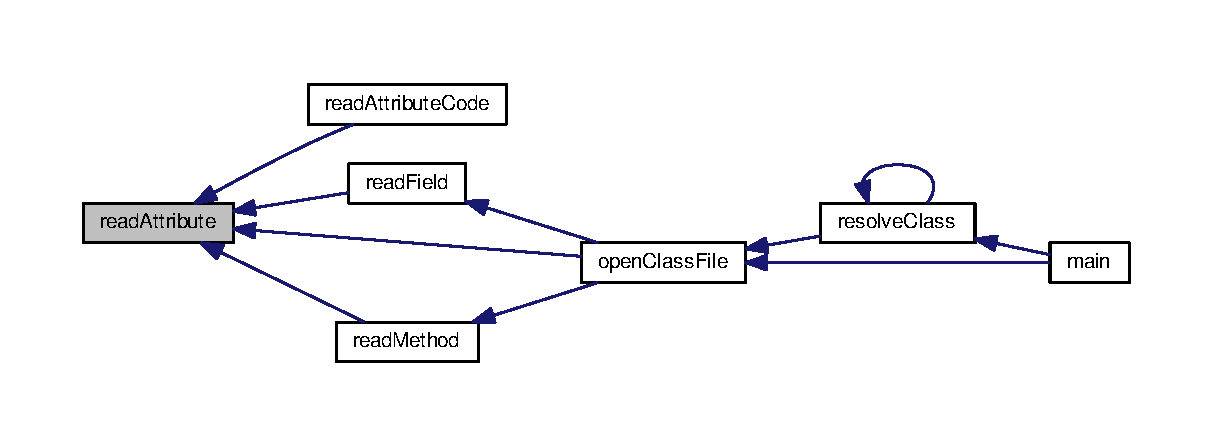
\includegraphics[width=350pt]{attributes_8h_a0aab7731ade76c16c2ff8b3bef1111d1_icgraph}
\end{center}
\end{figure}



\hypertarget{constantpool_8c}{}\section{Referência ao ficheiro src/constantpool.c}
\label{constantpool_8c}\index{src/constantpool.\+c@{src/constantpool.\+c}}
{\ttfamily \#include $<$stdlib.\+h$>$}\\*
{\ttfamily \#include $<$string.\+h$>$}\\*
{\ttfamily \#include $<$inttypes.\+h$>$}\\*
{\ttfamily \#include \char`\"{}readfunctions.\+h\char`\"{}}\\*
{\ttfamily \#include \char`\"{}constantpool.\+h\char`\"{}}\\*
{\ttfamily \#include \char`\"{}utf8.\+h\char`\"{}}\\*
Diagrama de dependências de inclusão para constantpool.\+c\+:\nopagebreak
\begin{figure}[H]
\begin{center}
\leavevmode
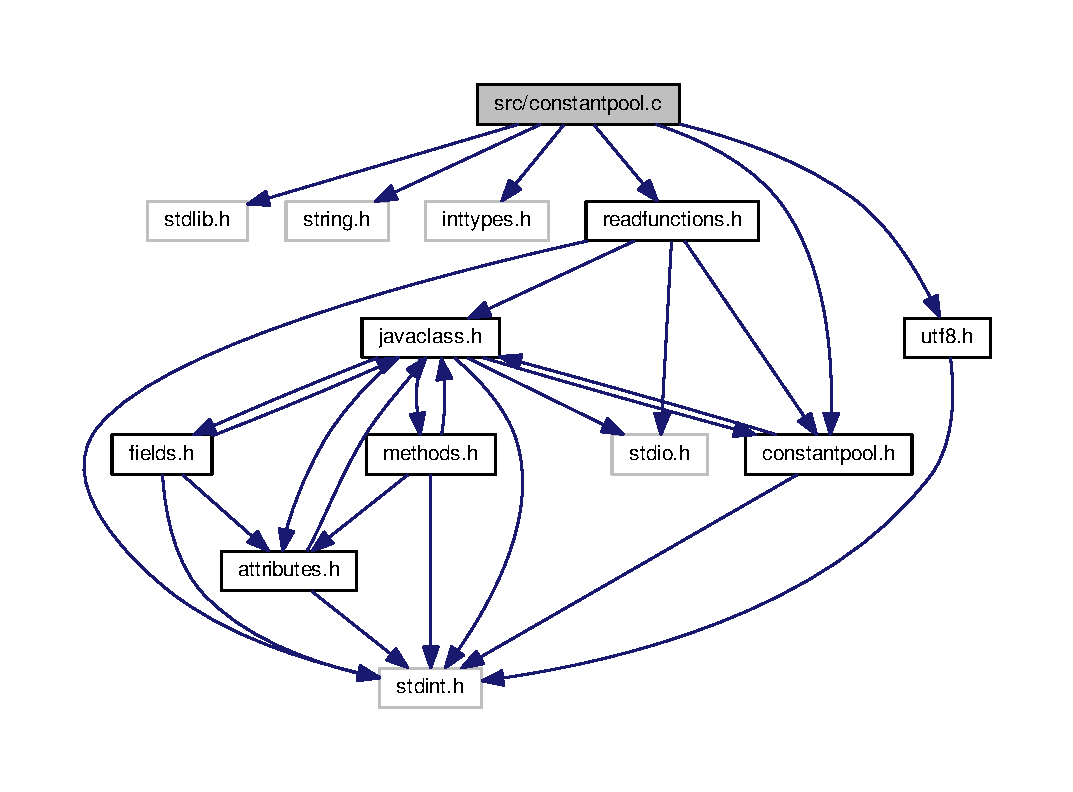
\includegraphics[width=350pt]{constantpool_8c__incl}
\end{center}
\end{figure}
\subsection*{Funções}
\begin{DoxyCompactItemize}
\item 
char \hyperlink{constantpool_8c_afea5409b47477cdbdb590472022c45f9}{read\+Constant\+Pool\+\_\+\+Class} (\hyperlink{structJavaClass}{Java\+Class} $\ast$jc, \hyperlink{structcp__info}{cp\+\_\+info} $\ast$entry)
\item 
char \hyperlink{constantpool_8c_ab3d1d9a9bdb1b7162d341ce9c8fd8784}{read\+Constant\+Pool\+\_\+\+Fieldref} (\hyperlink{structJavaClass}{Java\+Class} $\ast$jc, \hyperlink{structcp__info}{cp\+\_\+info} $\ast$entry)
\item 
char \hyperlink{constantpool_8c_a73f94285fc7c4790ca2900b6fc78b0f3}{read\+Constant\+Pool\+\_\+\+Integer} (\hyperlink{structJavaClass}{Java\+Class} $\ast$jc, \hyperlink{structcp__info}{cp\+\_\+info} $\ast$entry)
\item 
char \hyperlink{constantpool_8c_a1f4a6c4da0269e609a18f2d8174a2c39}{read\+Constant\+Pool\+\_\+\+Long} (\hyperlink{structJavaClass}{Java\+Class} $\ast$jc, \hyperlink{structcp__info}{cp\+\_\+info} $\ast$entry)
\item 
char \hyperlink{constantpool_8c_a730bf0dfa0b00508ed8ed3b6119853c3}{read\+Constant\+Pool\+\_\+\+Utf8} (\hyperlink{structJavaClass}{Java\+Class} $\ast$jc, \hyperlink{structcp__info}{cp\+\_\+info} $\ast$entry)
\item 
char \hyperlink{constantpool_8c_a62504539fde83f5183d20f262d4b1943}{read\+Constant\+Pool\+Entry} (\hyperlink{structJavaClass}{Java\+Class} $\ast$jc, \hyperlink{structcp__info}{cp\+\_\+info} $\ast$entry)
\item 
const char $\ast$ \hyperlink{constantpool_8c_a80f31089353a0ed2d861401c2c741701}{decode\+Tag} (uint8\+\_\+t tag)
\item 
void \hyperlink{constantpool_8c_a507c6272d8116f956bc75820b2c6ed23}{print\+Constant\+Pool\+Entry} (\hyperlink{structJavaClass}{Java\+Class} $\ast$jc, \hyperlink{structcp__info}{cp\+\_\+info} $\ast$entry)
\item 
void \hyperlink{constantpool_8c_ab7d27eb8d4164ae1a1fd11664ba4d1ef}{print\+Constant\+Pool} (\hyperlink{structJavaClass}{Java\+Class} $\ast$jc)
\end{DoxyCompactItemize}


\subsection{Documentação das funções}
\index{constantpool.\+c@{constantpool.\+c}!decode\+Tag@{decode\+Tag}}
\index{decode\+Tag@{decode\+Tag}!constantpool.\+c@{constantpool.\+c}}
\subsubsection[{\texorpdfstring{decode\+Tag(uint8\+\_\+t tag)}{decodeTag(uint8_t tag)}}]{\setlength{\rightskip}{0pt plus 5cm}const char$\ast$ decode\+Tag (
\begin{DoxyParamCaption}
\item[{uint8\+\_\+t}]{tag}
\end{DoxyParamCaption}
)}\hypertarget{constantpool_8c_a80f31089353a0ed2d861401c2c741701}{}\label{constantpool_8c_a80f31089353a0ed2d861401c2c741701}


Este é o diagrama das funções que utilizam esta função\+:\nopagebreak
\begin{figure}[H]
\begin{center}
\leavevmode
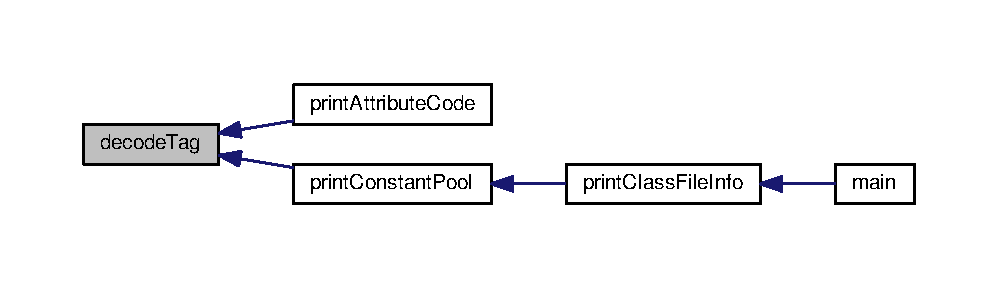
\includegraphics[width=350pt]{constantpool_8c_a80f31089353a0ed2d861401c2c741701_icgraph}
\end{center}
\end{figure}


\index{constantpool.\+c@{constantpool.\+c}!print\+Constant\+Pool@{print\+Constant\+Pool}}
\index{print\+Constant\+Pool@{print\+Constant\+Pool}!constantpool.\+c@{constantpool.\+c}}
\subsubsection[{\texorpdfstring{print\+Constant\+Pool(\+Java\+Class $\ast$jc)}{printConstantPool(JavaClass *jc)}}]{\setlength{\rightskip}{0pt plus 5cm}void print\+Constant\+Pool (
\begin{DoxyParamCaption}
\item[{{\bf Java\+Class} $\ast$}]{jc}
\end{DoxyParamCaption}
)}\hypertarget{constantpool_8c_ab7d27eb8d4164ae1a1fd11664ba4d1ef}{}\label{constantpool_8c_ab7d27eb8d4164ae1a1fd11664ba4d1ef}


Grafo de chamadas desta função\+:\nopagebreak
\begin{figure}[H]
\begin{center}
\leavevmode
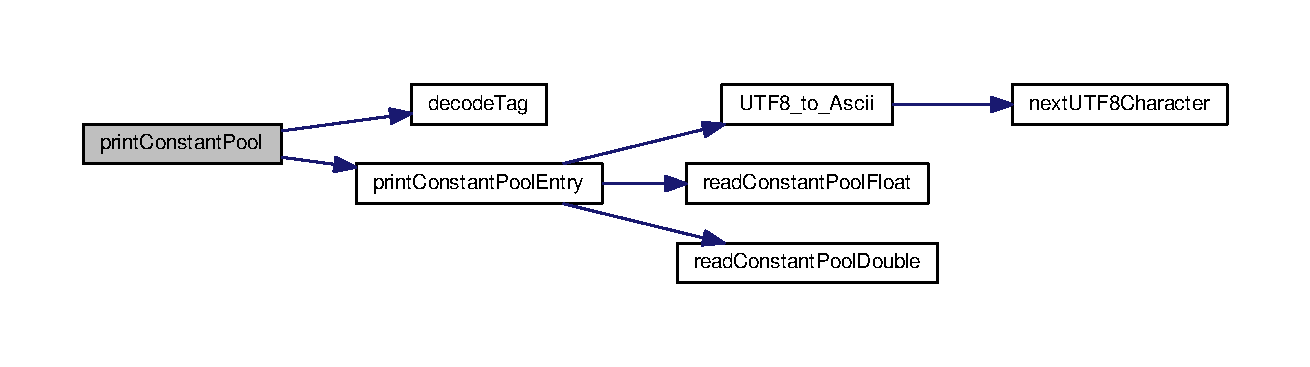
\includegraphics[width=350pt]{constantpool_8c_ab7d27eb8d4164ae1a1fd11664ba4d1ef_cgraph}
\end{center}
\end{figure}




Este é o diagrama das funções que utilizam esta função\+:\nopagebreak
\begin{figure}[H]
\begin{center}
\leavevmode
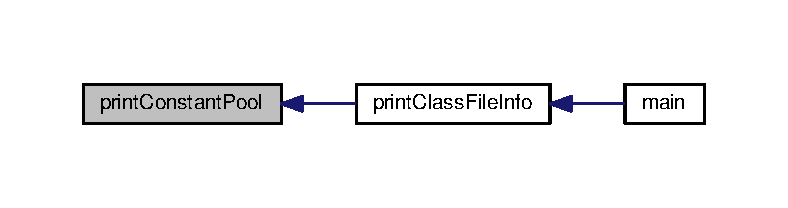
\includegraphics[width=350pt]{constantpool_8c_ab7d27eb8d4164ae1a1fd11664ba4d1ef_icgraph}
\end{center}
\end{figure}


\index{constantpool.\+c@{constantpool.\+c}!print\+Constant\+Pool\+Entry@{print\+Constant\+Pool\+Entry}}
\index{print\+Constant\+Pool\+Entry@{print\+Constant\+Pool\+Entry}!constantpool.\+c@{constantpool.\+c}}
\subsubsection[{\texorpdfstring{print\+Constant\+Pool\+Entry(\+Java\+Class $\ast$jc, cp\+\_\+info $\ast$entry)}{printConstantPoolEntry(JavaClass *jc, cp_info *entry)}}]{\setlength{\rightskip}{0pt plus 5cm}void print\+Constant\+Pool\+Entry (
\begin{DoxyParamCaption}
\item[{{\bf Java\+Class} $\ast$}]{jc, }
\item[{{\bf cp\+\_\+info} $\ast$}]{entry}
\end{DoxyParamCaption}
)}\hypertarget{constantpool_8c_a507c6272d8116f956bc75820b2c6ed23}{}\label{constantpool_8c_a507c6272d8116f956bc75820b2c6ed23}


Grafo de chamadas desta função\+:\nopagebreak
\begin{figure}[H]
\begin{center}
\leavevmode
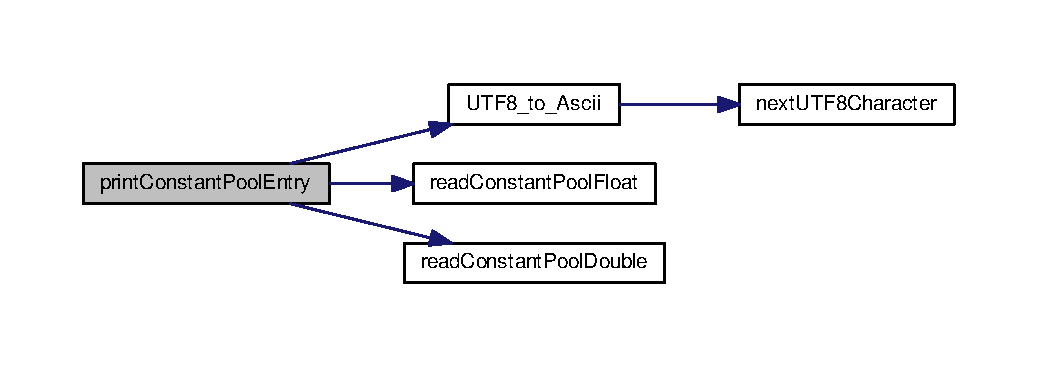
\includegraphics[width=350pt]{constantpool_8c_a507c6272d8116f956bc75820b2c6ed23_cgraph}
\end{center}
\end{figure}




Este é o diagrama das funções que utilizam esta função\+:\nopagebreak
\begin{figure}[H]
\begin{center}
\leavevmode
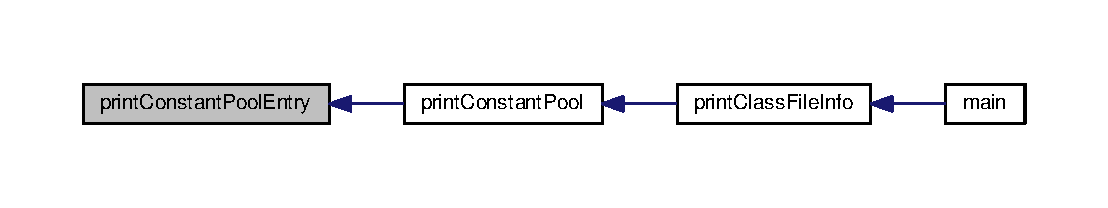
\includegraphics[width=350pt]{constantpool_8c_a507c6272d8116f956bc75820b2c6ed23_icgraph}
\end{center}
\end{figure}


\index{constantpool.\+c@{constantpool.\+c}!read\+Constant\+Pool\+\_\+\+Class@{read\+Constant\+Pool\+\_\+\+Class}}
\index{read\+Constant\+Pool\+\_\+\+Class@{read\+Constant\+Pool\+\_\+\+Class}!constantpool.\+c@{constantpool.\+c}}
\subsubsection[{\texorpdfstring{read\+Constant\+Pool\+\_\+\+Class(\+Java\+Class $\ast$jc, cp\+\_\+info $\ast$entry)}{readConstantPool_Class(JavaClass *jc, cp_info *entry)}}]{\setlength{\rightskip}{0pt plus 5cm}char read\+Constant\+Pool\+\_\+\+Class (
\begin{DoxyParamCaption}
\item[{{\bf Java\+Class} $\ast$}]{jc, }
\item[{{\bf cp\+\_\+info} $\ast$}]{entry}
\end{DoxyParamCaption}
)}\hypertarget{constantpool_8c_afea5409b47477cdbdb590472022c45f9}{}\label{constantpool_8c_afea5409b47477cdbdb590472022c45f9}


Grafo de chamadas desta função\+:\nopagebreak
\begin{figure}[H]
\begin{center}
\leavevmode
\includegraphics[width=287pt]{constantpool_8c_afea5409b47477cdbdb590472022c45f9_cgraph}
\end{center}
\end{figure}




Este é o diagrama das funções que utilizam esta função\+:\nopagebreak
\begin{figure}[H]
\begin{center}
\leavevmode
\includegraphics[width=350pt]{constantpool_8c_afea5409b47477cdbdb590472022c45f9_icgraph}
\end{center}
\end{figure}


\index{constantpool.\+c@{constantpool.\+c}!read\+Constant\+Pool\+\_\+\+Fieldref@{read\+Constant\+Pool\+\_\+\+Fieldref}}
\index{read\+Constant\+Pool\+\_\+\+Fieldref@{read\+Constant\+Pool\+\_\+\+Fieldref}!constantpool.\+c@{constantpool.\+c}}
\subsubsection[{\texorpdfstring{read\+Constant\+Pool\+\_\+\+Fieldref(\+Java\+Class $\ast$jc, cp\+\_\+info $\ast$entry)}{readConstantPool_Fieldref(JavaClass *jc, cp_info *entry)}}]{\setlength{\rightskip}{0pt plus 5cm}char read\+Constant\+Pool\+\_\+\+Fieldref (
\begin{DoxyParamCaption}
\item[{{\bf Java\+Class} $\ast$}]{jc, }
\item[{{\bf cp\+\_\+info} $\ast$}]{entry}
\end{DoxyParamCaption}
)}\hypertarget{constantpool_8c_ab3d1d9a9bdb1b7162d341ce9c8fd8784}{}\label{constantpool_8c_ab3d1d9a9bdb1b7162d341ce9c8fd8784}


Grafo de chamadas desta função\+:\nopagebreak
\begin{figure}[H]
\begin{center}
\leavevmode
\includegraphics[width=294pt]{constantpool_8c_ab3d1d9a9bdb1b7162d341ce9c8fd8784_cgraph}
\end{center}
\end{figure}




Este é o diagrama das funções que utilizam esta função\+:\nopagebreak
\begin{figure}[H]
\begin{center}
\leavevmode
\includegraphics[width=350pt]{constantpool_8c_ab3d1d9a9bdb1b7162d341ce9c8fd8784_icgraph}
\end{center}
\end{figure}


\index{constantpool.\+c@{constantpool.\+c}!read\+Constant\+Pool\+\_\+\+Integer@{read\+Constant\+Pool\+\_\+\+Integer}}
\index{read\+Constant\+Pool\+\_\+\+Integer@{read\+Constant\+Pool\+\_\+\+Integer}!constantpool.\+c@{constantpool.\+c}}
\subsubsection[{\texorpdfstring{read\+Constant\+Pool\+\_\+\+Integer(\+Java\+Class $\ast$jc, cp\+\_\+info $\ast$entry)}{readConstantPool_Integer(JavaClass *jc, cp_info *entry)}}]{\setlength{\rightskip}{0pt plus 5cm}char read\+Constant\+Pool\+\_\+\+Integer (
\begin{DoxyParamCaption}
\item[{{\bf Java\+Class} $\ast$}]{jc, }
\item[{{\bf cp\+\_\+info} $\ast$}]{entry}
\end{DoxyParamCaption}
)}\hypertarget{constantpool_8c_a73f94285fc7c4790ca2900b6fc78b0f3}{}\label{constantpool_8c_a73f94285fc7c4790ca2900b6fc78b0f3}


Grafo de chamadas desta função\+:\nopagebreak
\begin{figure}[H]
\begin{center}
\leavevmode
\includegraphics[width=292pt]{constantpool_8c_a73f94285fc7c4790ca2900b6fc78b0f3_cgraph}
\end{center}
\end{figure}




Este é o diagrama das funções que utilizam esta função\+:\nopagebreak
\begin{figure}[H]
\begin{center}
\leavevmode
\includegraphics[width=350pt]{constantpool_8c_a73f94285fc7c4790ca2900b6fc78b0f3_icgraph}
\end{center}
\end{figure}


\index{constantpool.\+c@{constantpool.\+c}!read\+Constant\+Pool\+\_\+\+Long@{read\+Constant\+Pool\+\_\+\+Long}}
\index{read\+Constant\+Pool\+\_\+\+Long@{read\+Constant\+Pool\+\_\+\+Long}!constantpool.\+c@{constantpool.\+c}}
\subsubsection[{\texorpdfstring{read\+Constant\+Pool\+\_\+\+Long(\+Java\+Class $\ast$jc, cp\+\_\+info $\ast$entry)}{readConstantPool_Long(JavaClass *jc, cp_info *entry)}}]{\setlength{\rightskip}{0pt plus 5cm}char read\+Constant\+Pool\+\_\+\+Long (
\begin{DoxyParamCaption}
\item[{{\bf Java\+Class} $\ast$}]{jc, }
\item[{{\bf cp\+\_\+info} $\ast$}]{entry}
\end{DoxyParamCaption}
)}\hypertarget{constantpool_8c_a1f4a6c4da0269e609a18f2d8174a2c39}{}\label{constantpool_8c_a1f4a6c4da0269e609a18f2d8174a2c39}


Grafo de chamadas desta função\+:\nopagebreak
\begin{figure}[H]
\begin{center}
\leavevmode
\includegraphics[width=283pt]{constantpool_8c_a1f4a6c4da0269e609a18f2d8174a2c39_cgraph}
\end{center}
\end{figure}




Este é o diagrama das funções que utilizam esta função\+:\nopagebreak
\begin{figure}[H]
\begin{center}
\leavevmode
\includegraphics[width=350pt]{constantpool_8c_a1f4a6c4da0269e609a18f2d8174a2c39_icgraph}
\end{center}
\end{figure}


\index{constantpool.\+c@{constantpool.\+c}!read\+Constant\+Pool\+\_\+\+Utf8@{read\+Constant\+Pool\+\_\+\+Utf8}}
\index{read\+Constant\+Pool\+\_\+\+Utf8@{read\+Constant\+Pool\+\_\+\+Utf8}!constantpool.\+c@{constantpool.\+c}}
\subsubsection[{\texorpdfstring{read\+Constant\+Pool\+\_\+\+Utf8(\+Java\+Class $\ast$jc, cp\+\_\+info $\ast$entry)}{readConstantPool_Utf8(JavaClass *jc, cp_info *entry)}}]{\setlength{\rightskip}{0pt plus 5cm}char read\+Constant\+Pool\+\_\+\+Utf8 (
\begin{DoxyParamCaption}
\item[{{\bf Java\+Class} $\ast$}]{jc, }
\item[{{\bf cp\+\_\+info} $\ast$}]{entry}
\end{DoxyParamCaption}
)}\hypertarget{constantpool_8c_a730bf0dfa0b00508ed8ed3b6119853c3}{}\label{constantpool_8c_a730bf0dfa0b00508ed8ed3b6119853c3}


Grafo de chamadas desta função\+:\nopagebreak
\begin{figure}[H]
\begin{center}
\leavevmode
\includegraphics[width=281pt]{constantpool_8c_a730bf0dfa0b00508ed8ed3b6119853c3_cgraph}
\end{center}
\end{figure}




Este é o diagrama das funções que utilizam esta função\+:\nopagebreak
\begin{figure}[H]
\begin{center}
\leavevmode
\includegraphics[width=350pt]{constantpool_8c_a730bf0dfa0b00508ed8ed3b6119853c3_icgraph}
\end{center}
\end{figure}


\index{constantpool.\+c@{constantpool.\+c}!read\+Constant\+Pool\+Entry@{read\+Constant\+Pool\+Entry}}
\index{read\+Constant\+Pool\+Entry@{read\+Constant\+Pool\+Entry}!constantpool.\+c@{constantpool.\+c}}
\subsubsection[{\texorpdfstring{read\+Constant\+Pool\+Entry(\+Java\+Class $\ast$jc, cp\+\_\+info $\ast$entry)}{readConstantPoolEntry(JavaClass *jc, cp_info *entry)}}]{\setlength{\rightskip}{0pt plus 5cm}char read\+Constant\+Pool\+Entry (
\begin{DoxyParamCaption}
\item[{{\bf Java\+Class} $\ast$}]{jc, }
\item[{{\bf cp\+\_\+info} $\ast$}]{entry}
\end{DoxyParamCaption}
)}\hypertarget{constantpool_8c_a62504539fde83f5183d20f262d4b1943}{}\label{constantpool_8c_a62504539fde83f5183d20f262d4b1943}


Grafo de chamadas desta função\+:\nopagebreak
\begin{figure}[H]
\begin{center}
\leavevmode
\includegraphics[width=350pt]{constantpool_8c_a62504539fde83f5183d20f262d4b1943_cgraph}
\end{center}
\end{figure}




Este é o diagrama das funções que utilizam esta função\+:\nopagebreak
\begin{figure}[H]
\begin{center}
\leavevmode
\includegraphics[width=350pt]{constantpool_8c_a62504539fde83f5183d20f262d4b1943_icgraph}
\end{center}
\end{figure}



\hypertarget{constantpool_8h}{}\section{Referência ao ficheiro src/constantpool.h}
\label{constantpool_8h}\index{src/constantpool.\+h@{src/constantpool.\+h}}
{\ttfamily \#include $<$stdint.\+h$>$}\\*
{\ttfamily \#include \char`\"{}javaclass.\+h\char`\"{}}\\*
Diagrama de dependências de inclusão para constantpool.\+h\+:\nopagebreak
\begin{figure}[H]
\begin{center}
\leavevmode
\includegraphics[width=350pt]{constantpool_8h__incl}
\end{center}
\end{figure}
Este grafo mostra quais são os ficheiros que incluem directamente ou indirectamente este ficheiro\+:\nopagebreak
\begin{figure}[H]
\begin{center}
\leavevmode
\includegraphics[width=350pt]{constantpool_8h__dep__incl}
\end{center}
\end{figure}
\subsection*{Estruturas de Dados}
\begin{DoxyCompactItemize}
\item 
struct \hyperlink{structcp__info}{cp\+\_\+info}
\end{DoxyCompactItemize}
\subsection*{Definições de tipos}
\begin{DoxyCompactItemize}
\item 
typedef struct \hyperlink{structcp__info}{cp\+\_\+info} \hyperlink{constantpool_8h_ac152ca02fa3b57b8d90f0ae0b30f099a}{cp\+\_\+info}
\end{DoxyCompactItemize}
\subsection*{Enumerações}
\begin{DoxyCompactItemize}
\item 
enum \hyperlink{constantpool_8h_a4a3344c6a9649978cbcf29955d4de3c3}{Constant\+Pool\+Tag} \{ \\*
\hyperlink{constantpool_8h_a4a3344c6a9649978cbcf29955d4de3c3a0c47012a59af298b394855447822a7e3}{C\+O\+N\+S\+T\+A\+N\+T\+\_\+\+Class} = 7, 
\hyperlink{constantpool_8h_a4a3344c6a9649978cbcf29955d4de3c3a6f435c620d73f5e9366149665dc8ec6e}{C\+O\+N\+S\+T\+A\+N\+T\+\_\+\+Fieldref} = 9, 
\hyperlink{constantpool_8h_a4a3344c6a9649978cbcf29955d4de3c3a74af7140e84140c938fbf89e0c33eea8}{C\+O\+N\+S\+T\+A\+N\+T\+\_\+\+Methodref} = 10, 
\hyperlink{constantpool_8h_a4a3344c6a9649978cbcf29955d4de3c3a49962b9b17bc2ab27647a398b8083828}{C\+O\+N\+S\+T\+A\+N\+T\+\_\+\+Interface\+Methodref} = 11, 
\\*
\hyperlink{constantpool_8h_a4a3344c6a9649978cbcf29955d4de3c3a2c4493d41b4f7ff5cf9f2846e1bb92e0}{C\+O\+N\+S\+T\+A\+N\+T\+\_\+\+String} = 8, 
\hyperlink{constantpool_8h_a4a3344c6a9649978cbcf29955d4de3c3a211cf9d5f5f1416862052d4671ad440f}{C\+O\+N\+S\+T\+A\+N\+T\+\_\+\+Integer} = 3, 
\hyperlink{constantpool_8h_a4a3344c6a9649978cbcf29955d4de3c3aaef0ceec2622d1d49b45fbe54e406f21}{C\+O\+N\+S\+T\+A\+N\+T\+\_\+\+Float} = 4, 
\hyperlink{constantpool_8h_a4a3344c6a9649978cbcf29955d4de3c3a1d98ddfe1f9abb18cf43bc2c1b74bdd5}{C\+O\+N\+S\+T\+A\+N\+T\+\_\+\+Long} = 5, 
\\*
\hyperlink{constantpool_8h_a4a3344c6a9649978cbcf29955d4de3c3a728b77a24433c54f6c8a0f613e50a2c5}{C\+O\+N\+S\+T\+A\+N\+T\+\_\+\+Double} = 6, 
\hyperlink{constantpool_8h_a4a3344c6a9649978cbcf29955d4de3c3a80805f21212baf2079b2ab767e2ab061}{C\+O\+N\+S\+T\+A\+N\+T\+\_\+\+Name\+And\+Type} = 12, 
\hyperlink{constantpool_8h_a4a3344c6a9649978cbcf29955d4de3c3a4100a823f09e364338e42951035432ed}{C\+O\+N\+S\+T\+A\+N\+T\+\_\+\+Utf8} = 1
 \}
\end{DoxyCompactItemize}
\subsection*{Funções}
\begin{DoxyCompactItemize}
\item 
const char $\ast$ \hyperlink{constantpool_8h_a80f31089353a0ed2d861401c2c741701}{decode\+Tag} (uint8\+\_\+t tag)
\item 
char \hyperlink{constantpool_8h_a62504539fde83f5183d20f262d4b1943}{read\+Constant\+Pool\+Entry} (\hyperlink{structJavaClass}{Java\+Class} $\ast$jc, \hyperlink{structcp__info}{cp\+\_\+info} $\ast$entry)
\item 
void \hyperlink{constantpool_8h_ab7d27eb8d4164ae1a1fd11664ba4d1ef}{print\+Constant\+Pool} (\hyperlink{structJavaClass}{Java\+Class} $\ast$jc)
\end{DoxyCompactItemize}


\subsection{Documentação dos tipos}
\index{constantpool.\+h@{constantpool.\+h}!cp\+\_\+info@{cp\+\_\+info}}
\index{cp\+\_\+info@{cp\+\_\+info}!constantpool.\+h@{constantpool.\+h}}
\subsubsection[{\texorpdfstring{cp\+\_\+info}{cp_info}}]{\setlength{\rightskip}{0pt plus 5cm}typedef struct {\bf cp\+\_\+info} {\bf cp\+\_\+info}}\hypertarget{constantpool_8h_ac152ca02fa3b57b8d90f0ae0b30f099a}{}\label{constantpool_8h_ac152ca02fa3b57b8d90f0ae0b30f099a}


\subsection{Documentação dos valores da enumeração}
\index{constantpool.\+h@{constantpool.\+h}!Constant\+Pool\+Tag@{Constant\+Pool\+Tag}}
\index{Constant\+Pool\+Tag@{Constant\+Pool\+Tag}!constantpool.\+h@{constantpool.\+h}}
\subsubsection[{\texorpdfstring{Constant\+Pool\+Tag}{ConstantPoolTag}}]{\setlength{\rightskip}{0pt plus 5cm}enum {\bf Constant\+Pool\+Tag}}\hypertarget{constantpool_8h_a4a3344c6a9649978cbcf29955d4de3c3}{}\label{constantpool_8h_a4a3344c6a9649978cbcf29955d4de3c3}
\begin{Desc}
\item[Valores de enumerações]\par
\begin{description}
\index{C\+O\+N\+S\+T\+A\+N\+T\+\_\+\+Class@{C\+O\+N\+S\+T\+A\+N\+T\+\_\+\+Class}!constantpool.\+h@{constantpool.\+h}}\index{constantpool.\+h@{constantpool.\+h}!C\+O\+N\+S\+T\+A\+N\+T\+\_\+\+Class@{C\+O\+N\+S\+T\+A\+N\+T\+\_\+\+Class}}\item[{\em 
C\+O\+N\+S\+T\+A\+N\+T\+\_\+\+Class\hypertarget{constantpool_8h_a4a3344c6a9649978cbcf29955d4de3c3a0c47012a59af298b394855447822a7e3}{}\label{constantpool_8h_a4a3344c6a9649978cbcf29955d4de3c3a0c47012a59af298b394855447822a7e3}
}]\index{C\+O\+N\+S\+T\+A\+N\+T\+\_\+\+Fieldref@{C\+O\+N\+S\+T\+A\+N\+T\+\_\+\+Fieldref}!constantpool.\+h@{constantpool.\+h}}\index{constantpool.\+h@{constantpool.\+h}!C\+O\+N\+S\+T\+A\+N\+T\+\_\+\+Fieldref@{C\+O\+N\+S\+T\+A\+N\+T\+\_\+\+Fieldref}}\item[{\em 
C\+O\+N\+S\+T\+A\+N\+T\+\_\+\+Fieldref\hypertarget{constantpool_8h_a4a3344c6a9649978cbcf29955d4de3c3a6f435c620d73f5e9366149665dc8ec6e}{}\label{constantpool_8h_a4a3344c6a9649978cbcf29955d4de3c3a6f435c620d73f5e9366149665dc8ec6e}
}]\index{C\+O\+N\+S\+T\+A\+N\+T\+\_\+\+Methodref@{C\+O\+N\+S\+T\+A\+N\+T\+\_\+\+Methodref}!constantpool.\+h@{constantpool.\+h}}\index{constantpool.\+h@{constantpool.\+h}!C\+O\+N\+S\+T\+A\+N\+T\+\_\+\+Methodref@{C\+O\+N\+S\+T\+A\+N\+T\+\_\+\+Methodref}}\item[{\em 
C\+O\+N\+S\+T\+A\+N\+T\+\_\+\+Methodref\hypertarget{constantpool_8h_a4a3344c6a9649978cbcf29955d4de3c3a74af7140e84140c938fbf89e0c33eea8}{}\label{constantpool_8h_a4a3344c6a9649978cbcf29955d4de3c3a74af7140e84140c938fbf89e0c33eea8}
}]\index{C\+O\+N\+S\+T\+A\+N\+T\+\_\+\+Interface\+Methodref@{C\+O\+N\+S\+T\+A\+N\+T\+\_\+\+Interface\+Methodref}!constantpool.\+h@{constantpool.\+h}}\index{constantpool.\+h@{constantpool.\+h}!C\+O\+N\+S\+T\+A\+N\+T\+\_\+\+Interface\+Methodref@{C\+O\+N\+S\+T\+A\+N\+T\+\_\+\+Interface\+Methodref}}\item[{\em 
C\+O\+N\+S\+T\+A\+N\+T\+\_\+\+Interface\+Methodref\hypertarget{constantpool_8h_a4a3344c6a9649978cbcf29955d4de3c3a49962b9b17bc2ab27647a398b8083828}{}\label{constantpool_8h_a4a3344c6a9649978cbcf29955d4de3c3a49962b9b17bc2ab27647a398b8083828}
}]\index{C\+O\+N\+S\+T\+A\+N\+T\+\_\+\+String@{C\+O\+N\+S\+T\+A\+N\+T\+\_\+\+String}!constantpool.\+h@{constantpool.\+h}}\index{constantpool.\+h@{constantpool.\+h}!C\+O\+N\+S\+T\+A\+N\+T\+\_\+\+String@{C\+O\+N\+S\+T\+A\+N\+T\+\_\+\+String}}\item[{\em 
C\+O\+N\+S\+T\+A\+N\+T\+\_\+\+String\hypertarget{constantpool_8h_a4a3344c6a9649978cbcf29955d4de3c3a2c4493d41b4f7ff5cf9f2846e1bb92e0}{}\label{constantpool_8h_a4a3344c6a9649978cbcf29955d4de3c3a2c4493d41b4f7ff5cf9f2846e1bb92e0}
}]\index{C\+O\+N\+S\+T\+A\+N\+T\+\_\+\+Integer@{C\+O\+N\+S\+T\+A\+N\+T\+\_\+\+Integer}!constantpool.\+h@{constantpool.\+h}}\index{constantpool.\+h@{constantpool.\+h}!C\+O\+N\+S\+T\+A\+N\+T\+\_\+\+Integer@{C\+O\+N\+S\+T\+A\+N\+T\+\_\+\+Integer}}\item[{\em 
C\+O\+N\+S\+T\+A\+N\+T\+\_\+\+Integer\hypertarget{constantpool_8h_a4a3344c6a9649978cbcf29955d4de3c3a211cf9d5f5f1416862052d4671ad440f}{}\label{constantpool_8h_a4a3344c6a9649978cbcf29955d4de3c3a211cf9d5f5f1416862052d4671ad440f}
}]\index{C\+O\+N\+S\+T\+A\+N\+T\+\_\+\+Float@{C\+O\+N\+S\+T\+A\+N\+T\+\_\+\+Float}!constantpool.\+h@{constantpool.\+h}}\index{constantpool.\+h@{constantpool.\+h}!C\+O\+N\+S\+T\+A\+N\+T\+\_\+\+Float@{C\+O\+N\+S\+T\+A\+N\+T\+\_\+\+Float}}\item[{\em 
C\+O\+N\+S\+T\+A\+N\+T\+\_\+\+Float\hypertarget{constantpool_8h_a4a3344c6a9649978cbcf29955d4de3c3aaef0ceec2622d1d49b45fbe54e406f21}{}\label{constantpool_8h_a4a3344c6a9649978cbcf29955d4de3c3aaef0ceec2622d1d49b45fbe54e406f21}
}]\index{C\+O\+N\+S\+T\+A\+N\+T\+\_\+\+Long@{C\+O\+N\+S\+T\+A\+N\+T\+\_\+\+Long}!constantpool.\+h@{constantpool.\+h}}\index{constantpool.\+h@{constantpool.\+h}!C\+O\+N\+S\+T\+A\+N\+T\+\_\+\+Long@{C\+O\+N\+S\+T\+A\+N\+T\+\_\+\+Long}}\item[{\em 
C\+O\+N\+S\+T\+A\+N\+T\+\_\+\+Long\hypertarget{constantpool_8h_a4a3344c6a9649978cbcf29955d4de3c3a1d98ddfe1f9abb18cf43bc2c1b74bdd5}{}\label{constantpool_8h_a4a3344c6a9649978cbcf29955d4de3c3a1d98ddfe1f9abb18cf43bc2c1b74bdd5}
}]\index{C\+O\+N\+S\+T\+A\+N\+T\+\_\+\+Double@{C\+O\+N\+S\+T\+A\+N\+T\+\_\+\+Double}!constantpool.\+h@{constantpool.\+h}}\index{constantpool.\+h@{constantpool.\+h}!C\+O\+N\+S\+T\+A\+N\+T\+\_\+\+Double@{C\+O\+N\+S\+T\+A\+N\+T\+\_\+\+Double}}\item[{\em 
C\+O\+N\+S\+T\+A\+N\+T\+\_\+\+Double\hypertarget{constantpool_8h_a4a3344c6a9649978cbcf29955d4de3c3a728b77a24433c54f6c8a0f613e50a2c5}{}\label{constantpool_8h_a4a3344c6a9649978cbcf29955d4de3c3a728b77a24433c54f6c8a0f613e50a2c5}
}]\index{C\+O\+N\+S\+T\+A\+N\+T\+\_\+\+Name\+And\+Type@{C\+O\+N\+S\+T\+A\+N\+T\+\_\+\+Name\+And\+Type}!constantpool.\+h@{constantpool.\+h}}\index{constantpool.\+h@{constantpool.\+h}!C\+O\+N\+S\+T\+A\+N\+T\+\_\+\+Name\+And\+Type@{C\+O\+N\+S\+T\+A\+N\+T\+\_\+\+Name\+And\+Type}}\item[{\em 
C\+O\+N\+S\+T\+A\+N\+T\+\_\+\+Name\+And\+Type\hypertarget{constantpool_8h_a4a3344c6a9649978cbcf29955d4de3c3a80805f21212baf2079b2ab767e2ab061}{}\label{constantpool_8h_a4a3344c6a9649978cbcf29955d4de3c3a80805f21212baf2079b2ab767e2ab061}
}]\index{C\+O\+N\+S\+T\+A\+N\+T\+\_\+\+Utf8@{C\+O\+N\+S\+T\+A\+N\+T\+\_\+\+Utf8}!constantpool.\+h@{constantpool.\+h}}\index{constantpool.\+h@{constantpool.\+h}!C\+O\+N\+S\+T\+A\+N\+T\+\_\+\+Utf8@{C\+O\+N\+S\+T\+A\+N\+T\+\_\+\+Utf8}}\item[{\em 
C\+O\+N\+S\+T\+A\+N\+T\+\_\+\+Utf8\hypertarget{constantpool_8h_a4a3344c6a9649978cbcf29955d4de3c3a4100a823f09e364338e42951035432ed}{}\label{constantpool_8h_a4a3344c6a9649978cbcf29955d4de3c3a4100a823f09e364338e42951035432ed}
}]\end{description}
\end{Desc}


\subsection{Documentação das funções}
\index{constantpool.\+h@{constantpool.\+h}!decode\+Tag@{decode\+Tag}}
\index{decode\+Tag@{decode\+Tag}!constantpool.\+h@{constantpool.\+h}}
\subsubsection[{\texorpdfstring{decode\+Tag(uint8\+\_\+t tag)}{decodeTag(uint8_t tag)}}]{\setlength{\rightskip}{0pt plus 5cm}const char$\ast$ decode\+Tag (
\begin{DoxyParamCaption}
\item[{uint8\+\_\+t}]{tag}
\end{DoxyParamCaption}
)}\hypertarget{constantpool_8h_a80f31089353a0ed2d861401c2c741701}{}\label{constantpool_8h_a80f31089353a0ed2d861401c2c741701}


Este é o diagrama das funções que utilizam esta função\+:\nopagebreak
\begin{figure}[H]
\begin{center}
\leavevmode
\includegraphics[width=350pt]{constantpool_8h_a80f31089353a0ed2d861401c2c741701_icgraph}
\end{center}
\end{figure}


\index{constantpool.\+h@{constantpool.\+h}!print\+Constant\+Pool@{print\+Constant\+Pool}}
\index{print\+Constant\+Pool@{print\+Constant\+Pool}!constantpool.\+h@{constantpool.\+h}}
\subsubsection[{\texorpdfstring{print\+Constant\+Pool(\+Java\+Class $\ast$jc)}{printConstantPool(JavaClass *jc)}}]{\setlength{\rightskip}{0pt plus 5cm}void print\+Constant\+Pool (
\begin{DoxyParamCaption}
\item[{{\bf Java\+Class} $\ast$}]{jc}
\end{DoxyParamCaption}
)}\hypertarget{constantpool_8h_ab7d27eb8d4164ae1a1fd11664ba4d1ef}{}\label{constantpool_8h_ab7d27eb8d4164ae1a1fd11664ba4d1ef}


Grafo de chamadas desta função\+:\nopagebreak
\begin{figure}[H]
\begin{center}
\leavevmode
\includegraphics[width=350pt]{constantpool_8h_ab7d27eb8d4164ae1a1fd11664ba4d1ef_cgraph}
\end{center}
\end{figure}




Este é o diagrama das funções que utilizam esta função\+:\nopagebreak
\begin{figure}[H]
\begin{center}
\leavevmode
\includegraphics[width=350pt]{constantpool_8h_ab7d27eb8d4164ae1a1fd11664ba4d1ef_icgraph}
\end{center}
\end{figure}


\index{constantpool.\+h@{constantpool.\+h}!read\+Constant\+Pool\+Entry@{read\+Constant\+Pool\+Entry}}
\index{read\+Constant\+Pool\+Entry@{read\+Constant\+Pool\+Entry}!constantpool.\+h@{constantpool.\+h}}
\subsubsection[{\texorpdfstring{read\+Constant\+Pool\+Entry(\+Java\+Class $\ast$jc, cp\+\_\+info $\ast$entry)}{readConstantPoolEntry(JavaClass *jc, cp_info *entry)}}]{\setlength{\rightskip}{0pt plus 5cm}char read\+Constant\+Pool\+Entry (
\begin{DoxyParamCaption}
\item[{{\bf Java\+Class} $\ast$}]{jc, }
\item[{{\bf cp\+\_\+info} $\ast$}]{entry}
\end{DoxyParamCaption}
)}\hypertarget{constantpool_8h_a62504539fde83f5183d20f262d4b1943}{}\label{constantpool_8h_a62504539fde83f5183d20f262d4b1943}


Grafo de chamadas desta função\+:\nopagebreak
\begin{figure}[H]
\begin{center}
\leavevmode
\includegraphics[width=350pt]{constantpool_8h_a62504539fde83f5183d20f262d4b1943_cgraph}
\end{center}
\end{figure}




Este é o diagrama das funções que utilizam esta função\+:\nopagebreak
\begin{figure}[H]
\begin{center}
\leavevmode
\includegraphics[width=350pt]{constantpool_8h_a62504539fde83f5183d20f262d4b1943_icgraph}
\end{center}
\end{figure}



\hypertarget{fields_8c}{}\section{Referência ao ficheiro src/fields.c}
\label{fields_8c}\index{src/fields.\+c@{src/fields.\+c}}
{\ttfamily \#include \char`\"{}fields.\+h\char`\"{}}\\*
{\ttfamily \#include \char`\"{}readfunctions.\+h\char`\"{}}\\*
{\ttfamily \#include \char`\"{}validity.\+h\char`\"{}}\\*
{\ttfamily \#include \char`\"{}utf8.\+h\char`\"{}}\\*
{\ttfamily \#include $<$stdlib.\+h$>$}\\*
Diagrama de dependências de inclusão para fields.\+c\+:\nopagebreak
\begin{figure}[H]
\begin{center}
\leavevmode
\includegraphics[width=350pt]{fields_8c__incl}
\end{center}
\end{figure}
\subsection*{Funções}
\begin{DoxyCompactItemize}
\item 
char \hyperlink{fields_8c_a5f94d9f571277dfd4d401b69ee8ce0f1}{read\+Field} (\hyperlink{structJavaClass}{Java\+Class} $\ast$jc, \hyperlink{structfield__info}{field\+\_\+info} $\ast$entry)
\item 
void \hyperlink{fields_8c_aeaafced8bc17d76aa18f38a005e01f99}{free\+Field\+Attributes} (\hyperlink{structfield__info}{field\+\_\+info} $\ast$entry)
\item 
void \hyperlink{fields_8c_a638dfd7ea9c1089e20de1ac871897ddf}{print\+All\+Fields} (\hyperlink{structJavaClass}{Java\+Class} $\ast$jc)
\end{DoxyCompactItemize}


\subsection{Documentação das funções}
\index{fields.\+c@{fields.\+c}!free\+Field\+Attributes@{free\+Field\+Attributes}}
\index{free\+Field\+Attributes@{free\+Field\+Attributes}!fields.\+c@{fields.\+c}}
\subsubsection[{\texorpdfstring{free\+Field\+Attributes(field\+\_\+info $\ast$entry)}{freeFieldAttributes(field_info *entry)}}]{\setlength{\rightskip}{0pt plus 5cm}void free\+Field\+Attributes (
\begin{DoxyParamCaption}
\item[{{\bf field\+\_\+info} $\ast$}]{entry}
\end{DoxyParamCaption}
)}\hypertarget{fields_8c_aeaafced8bc17d76aa18f38a005e01f99}{}\label{fields_8c_aeaafced8bc17d76aa18f38a005e01f99}


Grafo de chamadas desta função\+:\nopagebreak
\begin{figure}[H]
\begin{center}
\leavevmode
\includegraphics[width=298pt]{fields_8c_aeaafced8bc17d76aa18f38a005e01f99_cgraph}
\end{center}
\end{figure}




Este é o diagrama das funções que utilizam esta função\+:\nopagebreak
\begin{figure}[H]
\begin{center}
\leavevmode
\includegraphics[width=350pt]{fields_8c_aeaafced8bc17d76aa18f38a005e01f99_icgraph}
\end{center}
\end{figure}


\index{fields.\+c@{fields.\+c}!print\+All\+Fields@{print\+All\+Fields}}
\index{print\+All\+Fields@{print\+All\+Fields}!fields.\+c@{fields.\+c}}
\subsubsection[{\texorpdfstring{print\+All\+Fields(\+Java\+Class $\ast$jc)}{printAllFields(JavaClass *jc)}}]{\setlength{\rightskip}{0pt plus 5cm}void print\+All\+Fields (
\begin{DoxyParamCaption}
\item[{{\bf Java\+Class} $\ast$}]{jc}
\end{DoxyParamCaption}
)}\hypertarget{fields_8c_a638dfd7ea9c1089e20de1ac871897ddf}{}\label{fields_8c_a638dfd7ea9c1089e20de1ac871897ddf}


Grafo de chamadas desta função\+:\nopagebreak
\begin{figure}[H]
\begin{center}
\leavevmode
\includegraphics[width=350pt]{fields_8c_a638dfd7ea9c1089e20de1ac871897ddf_cgraph}
\end{center}
\end{figure}




Este é o diagrama das funções que utilizam esta função\+:\nopagebreak
\begin{figure}[H]
\begin{center}
\leavevmode
\includegraphics[width=350pt]{fields_8c_a638dfd7ea9c1089e20de1ac871897ddf_icgraph}
\end{center}
\end{figure}


\index{fields.\+c@{fields.\+c}!read\+Field@{read\+Field}}
\index{read\+Field@{read\+Field}!fields.\+c@{fields.\+c}}
\subsubsection[{\texorpdfstring{read\+Field(\+Java\+Class $\ast$jc, field\+\_\+info $\ast$entry)}{readField(JavaClass *jc, field_info *entry)}}]{\setlength{\rightskip}{0pt plus 5cm}char read\+Field (
\begin{DoxyParamCaption}
\item[{{\bf Java\+Class} $\ast$}]{jc, }
\item[{{\bf field\+\_\+info} $\ast$}]{entry}
\end{DoxyParamCaption}
)}\hypertarget{fields_8c_a5f94d9f571277dfd4d401b69ee8ce0f1}{}\label{fields_8c_a5f94d9f571277dfd4d401b69ee8ce0f1}


Grafo de chamadas desta função\+:\nopagebreak
\begin{figure}[H]
\begin{center}
\leavevmode
\includegraphics[width=350pt]{fields_8c_a5f94d9f571277dfd4d401b69ee8ce0f1_cgraph}
\end{center}
\end{figure}




Este é o diagrama das funções que utilizam esta função\+:\nopagebreak
\begin{figure}[H]
\begin{center}
\leavevmode
\includegraphics[width=350pt]{fields_8c_a5f94d9f571277dfd4d401b69ee8ce0f1_icgraph}
\end{center}
\end{figure}



\hypertarget{fields_8h}{}\section{Referência ao ficheiro src/fields.h}
\label{fields_8h}\index{src/fields.\+h@{src/fields.\+h}}
{\ttfamily \#include $<$stdint.\+h$>$}\\*
{\ttfamily \#include \char`\"{}javaclass.\+h\char`\"{}}\\*
{\ttfamily \#include \char`\"{}attributes.\+h\char`\"{}}\\*
Diagrama de dependências de inclusão para fields.\+h\+:\nopagebreak
\begin{figure}[H]
\begin{center}
\leavevmode
\includegraphics[width=350pt]{fields_8h__incl}
\end{center}
\end{figure}
Este grafo mostra quais são os ficheiros que incluem directamente ou indirectamente este ficheiro\+:\nopagebreak
\begin{figure}[H]
\begin{center}
\leavevmode
\includegraphics[width=350pt]{fields_8h__dep__incl}
\end{center}
\end{figure}
\subsection*{Estruturas de Dados}
\begin{DoxyCompactItemize}
\item 
struct \hyperlink{structfield__info}{field\+\_\+info}
\end{DoxyCompactItemize}
\subsection*{Definições de tipos}
\begin{DoxyCompactItemize}
\item 
typedef struct \hyperlink{structfield__info}{field\+\_\+info} \hyperlink{fields_8h_a92465becb59d258f61da663b1a202b14}{field\+\_\+info}
\end{DoxyCompactItemize}
\subsection*{Funções}
\begin{DoxyCompactItemize}
\item 
char \hyperlink{fields_8h_a5f94d9f571277dfd4d401b69ee8ce0f1}{read\+Field} (\hyperlink{structJavaClass}{Java\+Class} $\ast$jc, \hyperlink{structfield__info}{field\+\_\+info} $\ast$entry)
\item 
void \hyperlink{fields_8h_aeaafced8bc17d76aa18f38a005e01f99}{free\+Field\+Attributes} (\hyperlink{structfield__info}{field\+\_\+info} $\ast$entry)
\item 
void \hyperlink{fields_8h_a638dfd7ea9c1089e20de1ac871897ddf}{print\+All\+Fields} (\hyperlink{structJavaClass}{Java\+Class} $\ast$jc)
\end{DoxyCompactItemize}


\subsection{Documentação dos tipos}
\index{fields.\+h@{fields.\+h}!field\+\_\+info@{field\+\_\+info}}
\index{field\+\_\+info@{field\+\_\+info}!fields.\+h@{fields.\+h}}
\subsubsection[{\texorpdfstring{field\+\_\+info}{field_info}}]{\setlength{\rightskip}{0pt plus 5cm}typedef struct {\bf field\+\_\+info} {\bf field\+\_\+info}}\hypertarget{fields_8h_a92465becb59d258f61da663b1a202b14}{}\label{fields_8h_a92465becb59d258f61da663b1a202b14}


\subsection{Documentação das funções}
\index{fields.\+h@{fields.\+h}!free\+Field\+Attributes@{free\+Field\+Attributes}}
\index{free\+Field\+Attributes@{free\+Field\+Attributes}!fields.\+h@{fields.\+h}}
\subsubsection[{\texorpdfstring{free\+Field\+Attributes(field\+\_\+info $\ast$entry)}{freeFieldAttributes(field_info *entry)}}]{\setlength{\rightskip}{0pt plus 5cm}void free\+Field\+Attributes (
\begin{DoxyParamCaption}
\item[{{\bf field\+\_\+info} $\ast$}]{entry}
\end{DoxyParamCaption}
)}\hypertarget{fields_8h_aeaafced8bc17d76aa18f38a005e01f99}{}\label{fields_8h_aeaafced8bc17d76aa18f38a005e01f99}


Grafo de chamadas desta função\+:\nopagebreak
\begin{figure}[H]
\begin{center}
\leavevmode
\includegraphics[width=298pt]{fields_8h_aeaafced8bc17d76aa18f38a005e01f99_cgraph}
\end{center}
\end{figure}




Este é o diagrama das funções que utilizam esta função\+:\nopagebreak
\begin{figure}[H]
\begin{center}
\leavevmode
\includegraphics[width=350pt]{fields_8h_aeaafced8bc17d76aa18f38a005e01f99_icgraph}
\end{center}
\end{figure}


\index{fields.\+h@{fields.\+h}!print\+All\+Fields@{print\+All\+Fields}}
\index{print\+All\+Fields@{print\+All\+Fields}!fields.\+h@{fields.\+h}}
\subsubsection[{\texorpdfstring{print\+All\+Fields(\+Java\+Class $\ast$jc)}{printAllFields(JavaClass *jc)}}]{\setlength{\rightskip}{0pt plus 5cm}void print\+All\+Fields (
\begin{DoxyParamCaption}
\item[{{\bf Java\+Class} $\ast$}]{jc}
\end{DoxyParamCaption}
)}\hypertarget{fields_8h_a638dfd7ea9c1089e20de1ac871897ddf}{}\label{fields_8h_a638dfd7ea9c1089e20de1ac871897ddf}


Grafo de chamadas desta função\+:\nopagebreak
\begin{figure}[H]
\begin{center}
\leavevmode
\includegraphics[width=350pt]{fields_8h_a638dfd7ea9c1089e20de1ac871897ddf_cgraph}
\end{center}
\end{figure}




Este é o diagrama das funções que utilizam esta função\+:\nopagebreak
\begin{figure}[H]
\begin{center}
\leavevmode
\includegraphics[width=350pt]{fields_8h_a638dfd7ea9c1089e20de1ac871897ddf_icgraph}
\end{center}
\end{figure}


\index{fields.\+h@{fields.\+h}!read\+Field@{read\+Field}}
\index{read\+Field@{read\+Field}!fields.\+h@{fields.\+h}}
\subsubsection[{\texorpdfstring{read\+Field(\+Java\+Class $\ast$jc, field\+\_\+info $\ast$entry)}{readField(JavaClass *jc, field_info *entry)}}]{\setlength{\rightskip}{0pt plus 5cm}char read\+Field (
\begin{DoxyParamCaption}
\item[{{\bf Java\+Class} $\ast$}]{jc, }
\item[{{\bf field\+\_\+info} $\ast$}]{entry}
\end{DoxyParamCaption}
)}\hypertarget{fields_8h_a5f94d9f571277dfd4d401b69ee8ce0f1}{}\label{fields_8h_a5f94d9f571277dfd4d401b69ee8ce0f1}


Grafo de chamadas desta função\+:\nopagebreak
\begin{figure}[H]
\begin{center}
\leavevmode
\includegraphics[width=350pt]{fields_8h_a5f94d9f571277dfd4d401b69ee8ce0f1_cgraph}
\end{center}
\end{figure}




Este é o diagrama das funções que utilizam esta função\+:\nopagebreak
\begin{figure}[H]
\begin{center}
\leavevmode
\includegraphics[width=350pt]{fields_8h_a5f94d9f571277dfd4d401b69ee8ce0f1_icgraph}
\end{center}
\end{figure}



\hypertarget{framestack_8c}{}\section{Referência ao ficheiro src/framestack.c}
\label{framestack_8c}\index{src/framestack.\+c@{src/framestack.\+c}}
{\ttfamily \#include \char`\"{}framestack.\+h\char`\"{}}\\*
{\ttfamily \#include $<$stdlib.\+h$>$}\\*
Diagrama de dependências de inclusão para framestack.\+c\+:\nopagebreak
\begin{figure}[H]
\begin{center}
\leavevmode
\includegraphics[width=350pt]{framestack_8c__incl}
\end{center}
\end{figure}
\subsection*{Funções}
\begin{DoxyCompactItemize}
\item 
\hyperlink{structFrame}{Frame} $\ast$ \hyperlink{framestack_8c_a38bb1bda9e43d71c8472936c0ee14d72}{new\+Frame} (\hyperlink{structJavaClass}{Java\+Class} $\ast$jc, \hyperlink{structmethod__info}{method\+\_\+info} $\ast$method)
\item 
void \hyperlink{framestack_8c_ac6d7106961bbc47fa0f024aae9ab12f2}{free\+Frame} (\hyperlink{structFrame}{Frame} $\ast$frame)
\item 
uint8\+\_\+t \hyperlink{framestack_8c_a173f487de2e018f4d63d576edccb4c3d}{push\+Frame} (\hyperlink{structFrameStack}{Frame\+Stack} $\ast$$\ast$fs, \hyperlink{structFrame}{Frame} $\ast$frame)
\item 
uint8\+\_\+t \hyperlink{framestack_8c_ab279becc7f4fe166543e43d12e45ef56}{pop\+Frame} (\hyperlink{structFrameStack}{Frame\+Stack} $\ast$$\ast$fs, \hyperlink{structFrame}{Frame} $\ast$out\+Ptr)
\item 
void \hyperlink{framestack_8c_a6debf06c308367fb8e44acfdb0d27ea8}{free\+Frame\+Stack} (\hyperlink{structFrameStack}{Frame\+Stack} $\ast$$\ast$fs)
\end{DoxyCompactItemize}


\subsection{Documentação das funções}
\index{framestack.\+c@{framestack.\+c}!free\+Frame@{free\+Frame}}
\index{free\+Frame@{free\+Frame}!framestack.\+c@{framestack.\+c}}
\subsubsection[{\texorpdfstring{free\+Frame(\+Frame $\ast$frame)}{freeFrame(Frame *frame)}}]{\setlength{\rightskip}{0pt plus 5cm}void free\+Frame (
\begin{DoxyParamCaption}
\item[{{\bf Frame} $\ast$}]{frame}
\end{DoxyParamCaption}
)}\hypertarget{framestack_8c_ac6d7106961bbc47fa0f024aae9ab12f2}{}\label{framestack_8c_ac6d7106961bbc47fa0f024aae9ab12f2}


Grafo de chamadas desta função\+:\nopagebreak
\begin{figure}[H]
\begin{center}
\leavevmode
\includegraphics[width=272pt]{framestack_8c_ac6d7106961bbc47fa0f024aae9ab12f2_cgraph}
\end{center}
\end{figure}




Este é o diagrama das funções que utilizam esta função\+:\nopagebreak
\begin{figure}[H]
\begin{center}
\leavevmode
\includegraphics[width=350pt]{framestack_8c_ac6d7106961bbc47fa0f024aae9ab12f2_icgraph}
\end{center}
\end{figure}


\index{framestack.\+c@{framestack.\+c}!free\+Frame\+Stack@{free\+Frame\+Stack}}
\index{free\+Frame\+Stack@{free\+Frame\+Stack}!framestack.\+c@{framestack.\+c}}
\subsubsection[{\texorpdfstring{free\+Frame\+Stack(\+Frame\+Stack $\ast$$\ast$fs)}{freeFrameStack(FrameStack **fs)}}]{\setlength{\rightskip}{0pt plus 5cm}void free\+Frame\+Stack (
\begin{DoxyParamCaption}
\item[{{\bf Frame\+Stack} $\ast$$\ast$}]{fs}
\end{DoxyParamCaption}
)}\hypertarget{framestack_8c_a6debf06c308367fb8e44acfdb0d27ea8}{}\label{framestack_8c_a6debf06c308367fb8e44acfdb0d27ea8}


Grafo de chamadas desta função\+:\nopagebreak
\begin{figure}[H]
\begin{center}
\leavevmode
\includegraphics[width=350pt]{framestack_8c_a6debf06c308367fb8e44acfdb0d27ea8_cgraph}
\end{center}
\end{figure}




Este é o diagrama das funções que utilizam esta função\+:\nopagebreak
\begin{figure}[H]
\begin{center}
\leavevmode
\includegraphics[width=336pt]{framestack_8c_a6debf06c308367fb8e44acfdb0d27ea8_icgraph}
\end{center}
\end{figure}


\index{framestack.\+c@{framestack.\+c}!new\+Frame@{new\+Frame}}
\index{new\+Frame@{new\+Frame}!framestack.\+c@{framestack.\+c}}
\subsubsection[{\texorpdfstring{new\+Frame(\+Java\+Class $\ast$jc, method\+\_\+info $\ast$method)}{newFrame(JavaClass *jc, method_info *method)}}]{\setlength{\rightskip}{0pt plus 5cm}{\bf Frame}$\ast$ new\+Frame (
\begin{DoxyParamCaption}
\item[{{\bf Java\+Class} $\ast$}]{jc, }
\item[{{\bf method\+\_\+info} $\ast$}]{method}
\end{DoxyParamCaption}
)}\hypertarget{framestack_8c_a38bb1bda9e43d71c8472936c0ee14d72}{}\label{framestack_8c_a38bb1bda9e43d71c8472936c0ee14d72}


Grafo de chamadas desta função\+:\nopagebreak
\begin{figure}[H]
\begin{center}
\leavevmode
\includegraphics[width=279pt]{framestack_8c_a38bb1bda9e43d71c8472936c0ee14d72_cgraph}
\end{center}
\end{figure}




Este é o diagrama das funções que utilizam esta função\+:\nopagebreak
\begin{figure}[H]
\begin{center}
\leavevmode
\includegraphics[width=350pt]{framestack_8c_a38bb1bda9e43d71c8472936c0ee14d72_icgraph}
\end{center}
\end{figure}


\index{framestack.\+c@{framestack.\+c}!pop\+Frame@{pop\+Frame}}
\index{pop\+Frame@{pop\+Frame}!framestack.\+c@{framestack.\+c}}
\subsubsection[{\texorpdfstring{pop\+Frame(\+Frame\+Stack $\ast$$\ast$fs, Frame $\ast$out\+Ptr)}{popFrame(FrameStack **fs, Frame *outPtr)}}]{\setlength{\rightskip}{0pt plus 5cm}uint8\+\_\+t pop\+Frame (
\begin{DoxyParamCaption}
\item[{{\bf Frame\+Stack} $\ast$$\ast$}]{fs, }
\item[{{\bf Frame} $\ast$}]{out\+Ptr}
\end{DoxyParamCaption}
)}\hypertarget{framestack_8c_ab279becc7f4fe166543e43d12e45ef56}{}\label{framestack_8c_ab279becc7f4fe166543e43d12e45ef56}


Este é o diagrama das funções que utilizam esta função\+:\nopagebreak
\begin{figure}[H]
\begin{center}
\leavevmode
\includegraphics[width=350pt]{framestack_8c_ab279becc7f4fe166543e43d12e45ef56_icgraph}
\end{center}
\end{figure}


\index{framestack.\+c@{framestack.\+c}!push\+Frame@{push\+Frame}}
\index{push\+Frame@{push\+Frame}!framestack.\+c@{framestack.\+c}}
\subsubsection[{\texorpdfstring{push\+Frame(\+Frame\+Stack $\ast$$\ast$fs, Frame $\ast$frame)}{pushFrame(FrameStack **fs, Frame *frame)}}]{\setlength{\rightskip}{0pt plus 5cm}uint8\+\_\+t push\+Frame (
\begin{DoxyParamCaption}
\item[{{\bf Frame\+Stack} $\ast$$\ast$}]{fs, }
\item[{{\bf Frame} $\ast$}]{frame}
\end{DoxyParamCaption}
)}\hypertarget{framestack_8c_a173f487de2e018f4d63d576edccb4c3d}{}\label{framestack_8c_a173f487de2e018f4d63d576edccb4c3d}


Este é o diagrama das funções que utilizam esta função\+:\nopagebreak
\begin{figure}[H]
\begin{center}
\leavevmode
\includegraphics[width=350pt]{framestack_8c_a173f487de2e018f4d63d576edccb4c3d_icgraph}
\end{center}
\end{figure}



\hypertarget{framestack_8h}{}\section{Referência ao ficheiro src/framestack.h}
\label{framestack_8h}\index{src/framestack.\+h@{src/framestack.\+h}}
{\ttfamily \#include \char`\"{}operandstack.\+h\char`\"{}}\\*
{\ttfamily \#include \char`\"{}attributes.\+h\char`\"{}}\\*
Diagrama de dependências de inclusão para framestack.\+h\+:\nopagebreak
\begin{figure}[H]
\begin{center}
\leavevmode
\includegraphics[width=350pt]{framestack_8h__incl}
\end{center}
\end{figure}
Este grafo mostra quais são os ficheiros que incluem directamente ou indirectamente este ficheiro\+:\nopagebreak
\begin{figure}[H]
\begin{center}
\leavevmode
\includegraphics[width=350pt]{framestack_8h__dep__incl}
\end{center}
\end{figure}
\subsection*{Estruturas de Dados}
\begin{DoxyCompactItemize}
\item 
struct \hyperlink{structFrame}{Frame}
\item 
struct \hyperlink{structFrameStack}{Frame\+Stack}
\end{DoxyCompactItemize}
\subsection*{Definições de tipos}
\begin{DoxyCompactItemize}
\item 
typedef struct \hyperlink{structFrame}{Frame} \hyperlink{framestack_8h_a8bed1e36372ccc1470e37e91647cce20}{Frame}
\item 
typedef struct \hyperlink{structFrameStack}{Frame\+Stack} \hyperlink{framestack_8h_ab4bdf0a3d1b174c241124cb6b89dcaef}{Frame\+Stack}
\end{DoxyCompactItemize}
\subsection*{Funções}
\begin{DoxyCompactItemize}
\item 
\hyperlink{structFrame}{Frame} $\ast$ \hyperlink{framestack_8h_a38bb1bda9e43d71c8472936c0ee14d72}{new\+Frame} (\hyperlink{structJavaClass}{Java\+Class} $\ast$jc, \hyperlink{structmethod__info}{method\+\_\+info} $\ast$method)
\item 
void \hyperlink{framestack_8h_ac6d7106961bbc47fa0f024aae9ab12f2}{free\+Frame} (\hyperlink{structFrame}{Frame} $\ast$frame)
\item 
uint8\+\_\+t \hyperlink{framestack_8h_a173f487de2e018f4d63d576edccb4c3d}{push\+Frame} (\hyperlink{structFrameStack}{Frame\+Stack} $\ast$$\ast$fs, \hyperlink{structFrame}{Frame} $\ast$frame)
\item 
uint8\+\_\+t \hyperlink{framestack_8h_ab279becc7f4fe166543e43d12e45ef56}{pop\+Frame} (\hyperlink{structFrameStack}{Frame\+Stack} $\ast$$\ast$fs, \hyperlink{structFrame}{Frame} $\ast$out\+Ptr)
\item 
void \hyperlink{framestack_8h_a6debf06c308367fb8e44acfdb0d27ea8}{free\+Frame\+Stack} (\hyperlink{structFrameStack}{Frame\+Stack} $\ast$$\ast$fs)
\end{DoxyCompactItemize}


\subsection{Documentação dos tipos}
\index{framestack.\+h@{framestack.\+h}!Frame@{Frame}}
\index{Frame@{Frame}!framestack.\+h@{framestack.\+h}}
\subsubsection[{\texorpdfstring{Frame}{Frame}}]{\setlength{\rightskip}{0pt plus 5cm}typedef struct {\bf Frame} {\bf Frame}}\hypertarget{framestack_8h_a8bed1e36372ccc1470e37e91647cce20}{}\label{framestack_8h_a8bed1e36372ccc1470e37e91647cce20}
\index{framestack.\+h@{framestack.\+h}!Frame\+Stack@{Frame\+Stack}}
\index{Frame\+Stack@{Frame\+Stack}!framestack.\+h@{framestack.\+h}}
\subsubsection[{\texorpdfstring{Frame\+Stack}{FrameStack}}]{\setlength{\rightskip}{0pt plus 5cm}typedef struct {\bf Frame\+Stack} {\bf Frame\+Stack}}\hypertarget{framestack_8h_ab4bdf0a3d1b174c241124cb6b89dcaef}{}\label{framestack_8h_ab4bdf0a3d1b174c241124cb6b89dcaef}


\subsection{Documentação das funções}
\index{framestack.\+h@{framestack.\+h}!free\+Frame@{free\+Frame}}
\index{free\+Frame@{free\+Frame}!framestack.\+h@{framestack.\+h}}
\subsubsection[{\texorpdfstring{free\+Frame(\+Frame $\ast$frame)}{freeFrame(Frame *frame)}}]{\setlength{\rightskip}{0pt plus 5cm}void free\+Frame (
\begin{DoxyParamCaption}
\item[{{\bf Frame} $\ast$}]{frame}
\end{DoxyParamCaption}
)}\hypertarget{framestack_8h_ac6d7106961bbc47fa0f024aae9ab12f2}{}\label{framestack_8h_ac6d7106961bbc47fa0f024aae9ab12f2}


Grafo de chamadas desta função\+:\nopagebreak
\begin{figure}[H]
\begin{center}
\leavevmode
\includegraphics[width=272pt]{framestack_8h_ac6d7106961bbc47fa0f024aae9ab12f2_cgraph}
\end{center}
\end{figure}




Este é o diagrama das funções que utilizam esta função\+:\nopagebreak
\begin{figure}[H]
\begin{center}
\leavevmode
\includegraphics[width=350pt]{framestack_8h_ac6d7106961bbc47fa0f024aae9ab12f2_icgraph}
\end{center}
\end{figure}


\index{framestack.\+h@{framestack.\+h}!free\+Frame\+Stack@{free\+Frame\+Stack}}
\index{free\+Frame\+Stack@{free\+Frame\+Stack}!framestack.\+h@{framestack.\+h}}
\subsubsection[{\texorpdfstring{free\+Frame\+Stack(\+Frame\+Stack $\ast$$\ast$fs)}{freeFrameStack(FrameStack **fs)}}]{\setlength{\rightskip}{0pt plus 5cm}void free\+Frame\+Stack (
\begin{DoxyParamCaption}
\item[{{\bf Frame\+Stack} $\ast$$\ast$}]{fs}
\end{DoxyParamCaption}
)}\hypertarget{framestack_8h_a6debf06c308367fb8e44acfdb0d27ea8}{}\label{framestack_8h_a6debf06c308367fb8e44acfdb0d27ea8}


Grafo de chamadas desta função\+:\nopagebreak
\begin{figure}[H]
\begin{center}
\leavevmode
\includegraphics[width=350pt]{framestack_8h_a6debf06c308367fb8e44acfdb0d27ea8_cgraph}
\end{center}
\end{figure}




Este é o diagrama das funções que utilizam esta função\+:\nopagebreak
\begin{figure}[H]
\begin{center}
\leavevmode
\includegraphics[width=336pt]{framestack_8h_a6debf06c308367fb8e44acfdb0d27ea8_icgraph}
\end{center}
\end{figure}


\index{framestack.\+h@{framestack.\+h}!new\+Frame@{new\+Frame}}
\index{new\+Frame@{new\+Frame}!framestack.\+h@{framestack.\+h}}
\subsubsection[{\texorpdfstring{new\+Frame(\+Java\+Class $\ast$jc, method\+\_\+info $\ast$method)}{newFrame(JavaClass *jc, method_info *method)}}]{\setlength{\rightskip}{0pt plus 5cm}{\bf Frame}$\ast$ new\+Frame (
\begin{DoxyParamCaption}
\item[{{\bf Java\+Class} $\ast$}]{jc, }
\item[{{\bf method\+\_\+info} $\ast$}]{method}
\end{DoxyParamCaption}
)}\hypertarget{framestack_8h_a38bb1bda9e43d71c8472936c0ee14d72}{}\label{framestack_8h_a38bb1bda9e43d71c8472936c0ee14d72}


Grafo de chamadas desta função\+:\nopagebreak
\begin{figure}[H]
\begin{center}
\leavevmode
\includegraphics[width=279pt]{framestack_8h_a38bb1bda9e43d71c8472936c0ee14d72_cgraph}
\end{center}
\end{figure}




Este é o diagrama das funções que utilizam esta função\+:\nopagebreak
\begin{figure}[H]
\begin{center}
\leavevmode
\includegraphics[width=350pt]{framestack_8h_a38bb1bda9e43d71c8472936c0ee14d72_icgraph}
\end{center}
\end{figure}


\index{framestack.\+h@{framestack.\+h}!pop\+Frame@{pop\+Frame}}
\index{pop\+Frame@{pop\+Frame}!framestack.\+h@{framestack.\+h}}
\subsubsection[{\texorpdfstring{pop\+Frame(\+Frame\+Stack $\ast$$\ast$fs, Frame $\ast$out\+Ptr)}{popFrame(FrameStack **fs, Frame *outPtr)}}]{\setlength{\rightskip}{0pt plus 5cm}uint8\+\_\+t pop\+Frame (
\begin{DoxyParamCaption}
\item[{{\bf Frame\+Stack} $\ast$$\ast$}]{fs, }
\item[{{\bf Frame} $\ast$}]{out\+Ptr}
\end{DoxyParamCaption}
)}\hypertarget{framestack_8h_ab279becc7f4fe166543e43d12e45ef56}{}\label{framestack_8h_ab279becc7f4fe166543e43d12e45ef56}


Este é o diagrama das funções que utilizam esta função\+:\nopagebreak
\begin{figure}[H]
\begin{center}
\leavevmode
\includegraphics[width=350pt]{framestack_8h_ab279becc7f4fe166543e43d12e45ef56_icgraph}
\end{center}
\end{figure}


\index{framestack.\+h@{framestack.\+h}!push\+Frame@{push\+Frame}}
\index{push\+Frame@{push\+Frame}!framestack.\+h@{framestack.\+h}}
\subsubsection[{\texorpdfstring{push\+Frame(\+Frame\+Stack $\ast$$\ast$fs, Frame $\ast$frame)}{pushFrame(FrameStack **fs, Frame *frame)}}]{\setlength{\rightskip}{0pt plus 5cm}uint8\+\_\+t push\+Frame (
\begin{DoxyParamCaption}
\item[{{\bf Frame\+Stack} $\ast$$\ast$}]{fs, }
\item[{{\bf Frame} $\ast$}]{frame}
\end{DoxyParamCaption}
)}\hypertarget{framestack_8h_a173f487de2e018f4d63d576edccb4c3d}{}\label{framestack_8h_a173f487de2e018f4d63d576edccb4c3d}


Este é o diagrama das funções que utilizam esta função\+:\nopagebreak
\begin{figure}[H]
\begin{center}
\leavevmode
\includegraphics[width=350pt]{framestack_8h_a173f487de2e018f4d63d576edccb4c3d_icgraph}
\end{center}
\end{figure}



\hypertarget{instructions_8c}{}\section{Referência ao ficheiro src/instructions.c}
\label{instructions_8c}\index{src/instructions.\+c@{src/instructions.\+c}}
{\ttfamily \#include \char`\"{}instructions.\+h\char`\"{}}\\*
Diagrama de dependências de inclusão para instructions.\+c\+:\nopagebreak
\begin{figure}[H]
\begin{center}
\leavevmode
\includegraphics[width=350pt]{instructions_8c__incl}
\end{center}
\end{figure}
\subsection*{Macros}
\begin{DoxyCompactItemize}
\item 
\#define \hyperlink{instructions_8c_a9b9f3b0b1571f2d2dff832e9b083fd16}{D\+E\+C\+L\+R\+\_\+\+I\+C\+O\+N\+ST}(name,  value)
\item 
\#define \hyperlink{instructions_8c_a8e69952a93b261226fa33d711c534021}{D\+E\+C\+L\+R\+\_\+\+L\+C\+O\+N\+ST}(value)
\item 
\#define \hyperlink{instructions_8c_ac7802ed3e7d5a5ea8091c3169849601a}{D\+E\+C\+L\+R\+\_\+\+F\+C\+O\+N\+ST}(name,  value)
\item 
\#define \hyperlink{instructions_8c_ac4e91cad9d2eefa1b461177dbbeb4156}{D\+E\+C\+L\+R\+\_\+\+D\+C\+O\+N\+ST}(name,  high,  low)
\end{DoxyCompactItemize}
\subsection*{Funções}
\begin{DoxyCompactItemize}
\item 
uint8\+\_\+t \hyperlink{instructions_8c_a66a6ac26513b757e08d88b0ed26213a2}{instfunc\+\_\+nop} (\hyperlink{structJavaVirtualMachine}{Java\+Virtual\+Machine} $\ast$jvm, \hyperlink{structFrame}{Frame} $\ast$frame)
\item 
uint8\+\_\+t \hyperlink{instructions_8c_a39b87c11ed1110abbd8f8abe499f2ca8}{instfunc\+\_\+aconstnull} (\hyperlink{structJavaVirtualMachine}{Java\+Virtual\+Machine} $\ast$jvm, \hyperlink{structFrame}{Frame} $\ast$frame)
\item 
uint8\+\_\+t \hyperlink{instructions_8c_ab86139cde5e7ae97fc241a89339fe2e8}{instfunc\+\_\+bipush} (\hyperlink{structJavaVirtualMachine}{Java\+Virtual\+Machine} $\ast$jvm, \hyperlink{structFrame}{Frame} $\ast$frame)
\item 
uint8\+\_\+t \hyperlink{instructions_8c_a6d7c00376121a423c38eeccc0a3091b4}{instfunc\+\_\+sipush} (\hyperlink{structJavaVirtualMachine}{Java\+Virtual\+Machine} $\ast$jvm, \hyperlink{structFrame}{Frame} $\ast$frame)
\item 
uint8\+\_\+t \hyperlink{instructions_8c_a92d8f13080440d3079f1e5407b2f5f10}{instfunc\+\_\+ldc} (\hyperlink{structJavaVirtualMachine}{Java\+Virtual\+Machine} $\ast$jvm, \hyperlink{structFrame}{Frame} $\ast$frame)
\item 
\hyperlink{instructions_8h_ae8affa9babea747642d20877780599fa}{Instruction\+Function} \hyperlink{instructions_8c_a036f840d5a734d71a7807c8d4fc203c6}{fetch\+Opcode\+Function} (uint8\+\_\+t opcode)
\end{DoxyCompactItemize}


\subsection{Documentação das macros}
\index{instructions.\+c@{instructions.\+c}!D\+E\+C\+L\+R\+\_\+\+D\+C\+O\+N\+ST@{D\+E\+C\+L\+R\+\_\+\+D\+C\+O\+N\+ST}}
\index{D\+E\+C\+L\+R\+\_\+\+D\+C\+O\+N\+ST@{D\+E\+C\+L\+R\+\_\+\+D\+C\+O\+N\+ST}!instructions.\+c@{instructions.\+c}}
\subsubsection[{\texorpdfstring{D\+E\+C\+L\+R\+\_\+\+D\+C\+O\+N\+ST}{DECLR_DCONST}}]{\setlength{\rightskip}{0pt plus 5cm}\#define D\+E\+C\+L\+R\+\_\+\+D\+C\+O\+N\+ST(
\begin{DoxyParamCaption}
\item[{}]{name, }
\item[{}]{high, }
\item[{}]{low}
\end{DoxyParamCaption}
)}\hypertarget{instructions_8c_ac4e91cad9d2eefa1b461177dbbeb4156}{}\label{instructions_8c_ac4e91cad9d2eefa1b461177dbbeb4156}
{\bfseries Valor\+:}
\begin{DoxyCode}
uint8\_t instfunc\_dconst\_##name(\hyperlink{structJavaVirtualMachine}{JavaVirtualMachine}* jvm, \hyperlink{structFrame}{Frame}* frame) \(\backslash\)
    \{ \(\backslash\)
        if (!\hyperlink{operandstack_8c_a303eeaf9017d19267a875dd251fa2857}{pushOperand}(&frame->operands, high, \hyperlink{operandstack_8h_aa4b9b8291a90b1a586c468110fb346a4aa36f2949170ca1e708196ca721980275}{OP\_DOUBLE})) \(\backslash\)
        \{ \(\backslash\)
            jvm->status = \hyperlink{jvm_8h_a484d02331081db971c49ba36a1109967a005e0862fb18129abd7a2fe2be5bd932}{JVM\_STATUS\_OUT\_OF\_MEMORY}; \(\backslash\)
            return 0; \(\backslash\)
        \} \(\backslash\)
        if (!\hyperlink{operandstack_8c_a303eeaf9017d19267a875dd251fa2857}{pushOperand}(&frame->operands, low, \hyperlink{operandstack_8h_aa4b9b8291a90b1a586c468110fb346a4aa36f2949170ca1e708196ca721980275}{OP\_DOUBLE})) \(\backslash\)
        \{ \(\backslash\)
            jvm->status = \hyperlink{jvm_8h_a484d02331081db971c49ba36a1109967a005e0862fb18129abd7a2fe2be5bd932}{JVM\_STATUS\_OUT\_OF\_MEMORY}; \(\backslash\)
            return 0; \(\backslash\)
        \} \(\backslash\)
        return 1; \(\backslash\)
    \}
\end{DoxyCode}
\index{instructions.\+c@{instructions.\+c}!D\+E\+C\+L\+R\+\_\+\+F\+C\+O\+N\+ST@{D\+E\+C\+L\+R\+\_\+\+F\+C\+O\+N\+ST}}
\index{D\+E\+C\+L\+R\+\_\+\+F\+C\+O\+N\+ST@{D\+E\+C\+L\+R\+\_\+\+F\+C\+O\+N\+ST}!instructions.\+c@{instructions.\+c}}
\subsubsection[{\texorpdfstring{D\+E\+C\+L\+R\+\_\+\+F\+C\+O\+N\+ST}{DECLR_FCONST}}]{\setlength{\rightskip}{0pt plus 5cm}\#define D\+E\+C\+L\+R\+\_\+\+F\+C\+O\+N\+ST(
\begin{DoxyParamCaption}
\item[{}]{name, }
\item[{}]{value}
\end{DoxyParamCaption}
)}\hypertarget{instructions_8c_ac7802ed3e7d5a5ea8091c3169849601a}{}\label{instructions_8c_ac7802ed3e7d5a5ea8091c3169849601a}
{\bfseries Valor\+:}
\begin{DoxyCode}
uint8\_t instfunc\_fconst\_##name(\hyperlink{structJavaVirtualMachine}{JavaVirtualMachine}* jvm, \hyperlink{structFrame}{Frame}* frame) \(\backslash\)
    \{ \(\backslash\)
        if (!\hyperlink{operandstack_8c_a303eeaf9017d19267a875dd251fa2857}{pushOperand}(&frame->operands, \hyperlink{structOperandStack_a931d181370bfdb5b41edb8fe488c3b90}{value}, \hyperlink{operandstack_8h_aa4b9b8291a90b1a586c468110fb346a4ae0ed5f5c231ae95ba186cf99792ed418}{OP\_FLOAT})) \(\backslash\)
        \{ \(\backslash\)
            jvm->status = \hyperlink{jvm_8h_a484d02331081db971c49ba36a1109967a005e0862fb18129abd7a2fe2be5bd932}{JVM\_STATUS\_OUT\_OF\_MEMORY}; \(\backslash\)
            return 0; \(\backslash\)
        \} \(\backslash\)
        return 1; \(\backslash\)
    \}
\end{DoxyCode}
\index{instructions.\+c@{instructions.\+c}!D\+E\+C\+L\+R\+\_\+\+I\+C\+O\+N\+ST@{D\+E\+C\+L\+R\+\_\+\+I\+C\+O\+N\+ST}}
\index{D\+E\+C\+L\+R\+\_\+\+I\+C\+O\+N\+ST@{D\+E\+C\+L\+R\+\_\+\+I\+C\+O\+N\+ST}!instructions.\+c@{instructions.\+c}}
\subsubsection[{\texorpdfstring{D\+E\+C\+L\+R\+\_\+\+I\+C\+O\+N\+ST}{DECLR_ICONST}}]{\setlength{\rightskip}{0pt plus 5cm}\#define D\+E\+C\+L\+R\+\_\+\+I\+C\+O\+N\+ST(
\begin{DoxyParamCaption}
\item[{}]{name, }
\item[{}]{value}
\end{DoxyParamCaption}
)}\hypertarget{instructions_8c_a9b9f3b0b1571f2d2dff832e9b083fd16}{}\label{instructions_8c_a9b9f3b0b1571f2d2dff832e9b083fd16}
{\bfseries Valor\+:}
\begin{DoxyCode}
uint8\_t instfunc\_iconst\_##name(\hyperlink{structJavaVirtualMachine}{JavaVirtualMachine}* jvm, \hyperlink{structFrame}{Frame}* frame) \(\backslash\)
    \{ \(\backslash\)
        if (!\hyperlink{operandstack_8c_a303eeaf9017d19267a875dd251fa2857}{pushOperand}(&frame->operands, \hyperlink{structOperandStack_a931d181370bfdb5b41edb8fe488c3b90}{value}, \hyperlink{operandstack_8h_aa4b9b8291a90b1a586c468110fb346a4aa5087579d71722be9d06816518da2bc2}{OP\_INTEGER})) \(\backslash\)
        \{ \(\backslash\)
            jvm->status = \hyperlink{jvm_8h_a484d02331081db971c49ba36a1109967a005e0862fb18129abd7a2fe2be5bd932}{JVM\_STATUS\_OUT\_OF\_MEMORY}; \(\backslash\)
            return 0; \(\backslash\)
        \} \(\backslash\)
        return 1; \(\backslash\)
    \}
\end{DoxyCode}
\index{instructions.\+c@{instructions.\+c}!D\+E\+C\+L\+R\+\_\+\+L\+C\+O\+N\+ST@{D\+E\+C\+L\+R\+\_\+\+L\+C\+O\+N\+ST}}
\index{D\+E\+C\+L\+R\+\_\+\+L\+C\+O\+N\+ST@{D\+E\+C\+L\+R\+\_\+\+L\+C\+O\+N\+ST}!instructions.\+c@{instructions.\+c}}
\subsubsection[{\texorpdfstring{D\+E\+C\+L\+R\+\_\+\+L\+C\+O\+N\+ST}{DECLR_LCONST}}]{\setlength{\rightskip}{0pt plus 5cm}\#define D\+E\+C\+L\+R\+\_\+\+L\+C\+O\+N\+ST(
\begin{DoxyParamCaption}
\item[{}]{value}
\end{DoxyParamCaption}
)}\hypertarget{instructions_8c_a8e69952a93b261226fa33d711c534021}{}\label{instructions_8c_a8e69952a93b261226fa33d711c534021}
{\bfseries Valor\+:}
\begin{DoxyCode}
uint8\_t instfunc\_lconst\_##\hyperlink{structOperandStack_a931d181370bfdb5b41edb8fe488c3b90}{value}(\hyperlink{structJavaVirtualMachine}{JavaVirtualMachine}* jvm, 
      \hyperlink{structFrame}{Frame}* frame) \(\backslash\)
    \{ \(\backslash\)
        if (!\hyperlink{operandstack_8c_a303eeaf9017d19267a875dd251fa2857}{pushOperand}(&frame->operands, 0, \hyperlink{operandstack_8h_aa4b9b8291a90b1a586c468110fb346a4a2069b5f7fac5141a8c24357fde7fe026}{OP\_LONG})) \(\backslash\)
        \{ \(\backslash\)
            jvm->status = \hyperlink{jvm_8h_a484d02331081db971c49ba36a1109967a005e0862fb18129abd7a2fe2be5bd932}{JVM\_STATUS\_OUT\_OF\_MEMORY}; \(\backslash\)
            return 0; \(\backslash\)
        \} \(\backslash\)
        if (!\hyperlink{operandstack_8c_a303eeaf9017d19267a875dd251fa2857}{pushOperand}(&frame->operands, \hyperlink{structOperandStack_a931d181370bfdb5b41edb8fe488c3b90}{value}, \hyperlink{operandstack_8h_aa4b9b8291a90b1a586c468110fb346a4a2069b5f7fac5141a8c24357fde7fe026}{OP\_LONG})) \(\backslash\)
        \{ \(\backslash\)
            jvm->status = \hyperlink{jvm_8h_a484d02331081db971c49ba36a1109967a005e0862fb18129abd7a2fe2be5bd932}{JVM\_STATUS\_OUT\_OF\_MEMORY}; \(\backslash\)
            return 0; \(\backslash\)
        \} \(\backslash\)
        return 1; \(\backslash\)
    \}
\end{DoxyCode}


\subsection{Documentação das funções}
\index{instructions.\+c@{instructions.\+c}!fetch\+Opcode\+Function@{fetch\+Opcode\+Function}}
\index{fetch\+Opcode\+Function@{fetch\+Opcode\+Function}!instructions.\+c@{instructions.\+c}}
\subsubsection[{\texorpdfstring{fetch\+Opcode\+Function(uint8\+\_\+t opcode)}{fetchOpcodeFunction(uint8_t opcode)}}]{\setlength{\rightskip}{0pt plus 5cm}{\bf Instruction\+Function} fetch\+Opcode\+Function (
\begin{DoxyParamCaption}
\item[{uint8\+\_\+t}]{opcode}
\end{DoxyParamCaption}
)}\hypertarget{instructions_8c_a036f840d5a734d71a7807c8d4fc203c6}{}\label{instructions_8c_a036f840d5a734d71a7807c8d4fc203c6}


Grafo de chamadas desta função\+:\nopagebreak
\begin{figure}[H]
\begin{center}
\leavevmode
\includegraphics[width=350pt]{instructions_8c_a036f840d5a734d71a7807c8d4fc203c6_cgraph}
\end{center}
\end{figure}




Este é o diagrama das funções que utilizam esta função\+:\nopagebreak
\begin{figure}[H]
\begin{center}
\leavevmode
\includegraphics[width=350pt]{instructions_8c_a036f840d5a734d71a7807c8d4fc203c6_icgraph}
\end{center}
\end{figure}


\index{instructions.\+c@{instructions.\+c}!instfunc\+\_\+aconstnull@{instfunc\+\_\+aconstnull}}
\index{instfunc\+\_\+aconstnull@{instfunc\+\_\+aconstnull}!instructions.\+c@{instructions.\+c}}
\subsubsection[{\texorpdfstring{instfunc\+\_\+aconstnull(\+Java\+Virtual\+Machine $\ast$jvm, Frame $\ast$frame)}{instfunc_aconstnull(JavaVirtualMachine *jvm, Frame *frame)}}]{\setlength{\rightskip}{0pt plus 5cm}uint8\+\_\+t instfunc\+\_\+aconstnull (
\begin{DoxyParamCaption}
\item[{{\bf Java\+Virtual\+Machine} $\ast$}]{jvm, }
\item[{{\bf Frame} $\ast$}]{frame}
\end{DoxyParamCaption}
)}\hypertarget{instructions_8c_a39b87c11ed1110abbd8f8abe499f2ca8}{}\label{instructions_8c_a39b87c11ed1110abbd8f8abe499f2ca8}


Grafo de chamadas desta função\+:\nopagebreak
\begin{figure}[H]
\begin{center}
\leavevmode
\includegraphics[width=291pt]{instructions_8c_a39b87c11ed1110abbd8f8abe499f2ca8_cgraph}
\end{center}
\end{figure}




Este é o diagrama das funções que utilizam esta função\+:\nopagebreak
\begin{figure}[H]
\begin{center}
\leavevmode
\includegraphics[width=350pt]{instructions_8c_a39b87c11ed1110abbd8f8abe499f2ca8_icgraph}
\end{center}
\end{figure}


\index{instructions.\+c@{instructions.\+c}!instfunc\+\_\+bipush@{instfunc\+\_\+bipush}}
\index{instfunc\+\_\+bipush@{instfunc\+\_\+bipush}!instructions.\+c@{instructions.\+c}}
\subsubsection[{\texorpdfstring{instfunc\+\_\+bipush(\+Java\+Virtual\+Machine $\ast$jvm, Frame $\ast$frame)}{instfunc_bipush(JavaVirtualMachine *jvm, Frame *frame)}}]{\setlength{\rightskip}{0pt plus 5cm}uint8\+\_\+t instfunc\+\_\+bipush (
\begin{DoxyParamCaption}
\item[{{\bf Java\+Virtual\+Machine} $\ast$}]{jvm, }
\item[{{\bf Frame} $\ast$}]{frame}
\end{DoxyParamCaption}
)}\hypertarget{instructions_8c_ab86139cde5e7ae97fc241a89339fe2e8}{}\label{instructions_8c_ab86139cde5e7ae97fc241a89339fe2e8}


Grafo de chamadas desta função\+:\nopagebreak
\begin{figure}[H]
\begin{center}
\leavevmode
\includegraphics[width=275pt]{instructions_8c_ab86139cde5e7ae97fc241a89339fe2e8_cgraph}
\end{center}
\end{figure}




Este é o diagrama das funções que utilizam esta função\+:\nopagebreak
\begin{figure}[H]
\begin{center}
\leavevmode
\includegraphics[width=350pt]{instructions_8c_ab86139cde5e7ae97fc241a89339fe2e8_icgraph}
\end{center}
\end{figure}


\index{instructions.\+c@{instructions.\+c}!instfunc\+\_\+ldc@{instfunc\+\_\+ldc}}
\index{instfunc\+\_\+ldc@{instfunc\+\_\+ldc}!instructions.\+c@{instructions.\+c}}
\subsubsection[{\texorpdfstring{instfunc\+\_\+ldc(\+Java\+Virtual\+Machine $\ast$jvm, Frame $\ast$frame)}{instfunc_ldc(JavaVirtualMachine *jvm, Frame *frame)}}]{\setlength{\rightskip}{0pt plus 5cm}uint8\+\_\+t instfunc\+\_\+ldc (
\begin{DoxyParamCaption}
\item[{{\bf Java\+Virtual\+Machine} $\ast$}]{jvm, }
\item[{{\bf Frame} $\ast$}]{frame}
\end{DoxyParamCaption}
)}\hypertarget{instructions_8c_a92d8f13080440d3079f1e5407b2f5f10}{}\label{instructions_8c_a92d8f13080440d3079f1e5407b2f5f10}


Grafo de chamadas desta função\+:\nopagebreak
\begin{figure}[H]
\begin{center}
\leavevmode
\includegraphics[width=259pt]{instructions_8c_a92d8f13080440d3079f1e5407b2f5f10_cgraph}
\end{center}
\end{figure}




Este é o diagrama das funções que utilizam esta função\+:\nopagebreak
\begin{figure}[H]
\begin{center}
\leavevmode
\includegraphics[width=350pt]{instructions_8c_a92d8f13080440d3079f1e5407b2f5f10_icgraph}
\end{center}
\end{figure}


\index{instructions.\+c@{instructions.\+c}!instfunc\+\_\+nop@{instfunc\+\_\+nop}}
\index{instfunc\+\_\+nop@{instfunc\+\_\+nop}!instructions.\+c@{instructions.\+c}}
\subsubsection[{\texorpdfstring{instfunc\+\_\+nop(\+Java\+Virtual\+Machine $\ast$jvm, Frame $\ast$frame)}{instfunc_nop(JavaVirtualMachine *jvm, Frame *frame)}}]{\setlength{\rightskip}{0pt plus 5cm}uint8\+\_\+t instfunc\+\_\+nop (
\begin{DoxyParamCaption}
\item[{{\bf Java\+Virtual\+Machine} $\ast$}]{jvm, }
\item[{{\bf Frame} $\ast$}]{frame}
\end{DoxyParamCaption}
)}\hypertarget{instructions_8c_a66a6ac26513b757e08d88b0ed26213a2}{}\label{instructions_8c_a66a6ac26513b757e08d88b0ed26213a2}


Este é o diagrama das funções que utilizam esta função\+:\nopagebreak
\begin{figure}[H]
\begin{center}
\leavevmode
\includegraphics[width=350pt]{instructions_8c_a66a6ac26513b757e08d88b0ed26213a2_icgraph}
\end{center}
\end{figure}


\index{instructions.\+c@{instructions.\+c}!instfunc\+\_\+sipush@{instfunc\+\_\+sipush}}
\index{instfunc\+\_\+sipush@{instfunc\+\_\+sipush}!instructions.\+c@{instructions.\+c}}
\subsubsection[{\texorpdfstring{instfunc\+\_\+sipush(\+Java\+Virtual\+Machine $\ast$jvm, Frame $\ast$frame)}{instfunc_sipush(JavaVirtualMachine *jvm, Frame *frame)}}]{\setlength{\rightskip}{0pt plus 5cm}uint8\+\_\+t instfunc\+\_\+sipush (
\begin{DoxyParamCaption}
\item[{{\bf Java\+Virtual\+Machine} $\ast$}]{jvm, }
\item[{{\bf Frame} $\ast$}]{frame}
\end{DoxyParamCaption}
)}\hypertarget{instructions_8c_a6d7c00376121a423c38eeccc0a3091b4}{}\label{instructions_8c_a6d7c00376121a423c38eeccc0a3091b4}


Grafo de chamadas desta função\+:\nopagebreak
\begin{figure}[H]
\begin{center}
\leavevmode
\includegraphics[width=275pt]{instructions_8c_a6d7c00376121a423c38eeccc0a3091b4_cgraph}
\end{center}
\end{figure}




Este é o diagrama das funções que utilizam esta função\+:\nopagebreak
\begin{figure}[H]
\begin{center}
\leavevmode
\includegraphics[width=350pt]{instructions_8c_a6d7c00376121a423c38eeccc0a3091b4_icgraph}
\end{center}
\end{figure}



\hypertarget{instructions_8h}{}\section{Referência ao ficheiro src/instructions.h}
\label{instructions_8h}\index{src/instructions.\+h@{src/instructions.\+h}}
{\ttfamily \#include $<$stdlib.\+h$>$}\\*
{\ttfamily \#include $<$stdint.\+h$>$}\\*
{\ttfamily \#include \char`\"{}jvm.\+h\char`\"{}}\\*
{\ttfamily \#include \char`\"{}framestack.\+h\char`\"{}}\\*
Diagrama de dependências de inclusão para instructions.\+h\+:\nopagebreak
\begin{figure}[H]
\begin{center}
\leavevmode
\includegraphics[width=350pt]{instructions_8h__incl}
\end{center}
\end{figure}
Este grafo mostra quais são os ficheiros que incluem directamente ou indirectamente este ficheiro\+:\nopagebreak
\begin{figure}[H]
\begin{center}
\leavevmode
\includegraphics[width=248pt]{instructions_8h__dep__incl}
\end{center}
\end{figure}
\subsection*{Definições de tipos}
\begin{DoxyCompactItemize}
\item 
typedef uint8\+\_\+t($\ast$ \hyperlink{instructions_8h_ae8affa9babea747642d20877780599fa}{Instruction\+Function}) (\hyperlink{structJavaVirtualMachine}{Java\+Virtual\+Machine} $\ast$jvm, \hyperlink{structFrame}{Frame} $\ast$current\+Frame)
\end{DoxyCompactItemize}
\subsection*{Funções}
\begin{DoxyCompactItemize}
\item 
\hyperlink{instructions_8h_ae8affa9babea747642d20877780599fa}{Instruction\+Function} \hyperlink{instructions_8h_a036f840d5a734d71a7807c8d4fc203c6}{fetch\+Opcode\+Function} (uint8\+\_\+t opcode)
\end{DoxyCompactItemize}


\subsection{Documentação dos tipos}
\index{instructions.\+h@{instructions.\+h}!Instruction\+Function@{Instruction\+Function}}
\index{Instruction\+Function@{Instruction\+Function}!instructions.\+h@{instructions.\+h}}
\subsubsection[{\texorpdfstring{Instruction\+Function}{InstructionFunction}}]{\setlength{\rightskip}{0pt plus 5cm}typedef uint8\+\_\+t($\ast$ Instruction\+Function) ({\bf Java\+Virtual\+Machine} $\ast$jvm, {\bf Frame} $\ast$current\+Frame)}\hypertarget{instructions_8h_ae8affa9babea747642d20877780599fa}{}\label{instructions_8h_ae8affa9babea747642d20877780599fa}


\subsection{Documentação das funções}
\index{instructions.\+h@{instructions.\+h}!fetch\+Opcode\+Function@{fetch\+Opcode\+Function}}
\index{fetch\+Opcode\+Function@{fetch\+Opcode\+Function}!instructions.\+h@{instructions.\+h}}
\subsubsection[{\texorpdfstring{fetch\+Opcode\+Function(uint8\+\_\+t opcode)}{fetchOpcodeFunction(uint8_t opcode)}}]{\setlength{\rightskip}{0pt plus 5cm}{\bf Instruction\+Function} fetch\+Opcode\+Function (
\begin{DoxyParamCaption}
\item[{uint8\+\_\+t}]{opcode}
\end{DoxyParamCaption}
)}\hypertarget{instructions_8h_a036f840d5a734d71a7807c8d4fc203c6}{}\label{instructions_8h_a036f840d5a734d71a7807c8d4fc203c6}


Grafo de chamadas desta função\+:\nopagebreak
\begin{figure}[H]
\begin{center}
\leavevmode
\includegraphics[width=350pt]{instructions_8h_a036f840d5a734d71a7807c8d4fc203c6_cgraph}
\end{center}
\end{figure}




Este é o diagrama das funções que utilizam esta função\+:\nopagebreak
\begin{figure}[H]
\begin{center}
\leavevmode
\includegraphics[width=350pt]{instructions_8h_a036f840d5a734d71a7807c8d4fc203c6_icgraph}
\end{center}
\end{figure}



\hypertarget{javaclass_8c}{}\section{Referência ao ficheiro src/javaclass.c}
\label{javaclass_8c}\index{src/javaclass.\+c@{src/javaclass.\+c}}
{\ttfamily \#include \char`\"{}readfunctions.\+h\char`\"{}}\\*
{\ttfamily \#include \char`\"{}javaclass.\+h\char`\"{}}\\*
{\ttfamily \#include \char`\"{}constantpool.\+h\char`\"{}}\\*
{\ttfamily \#include \char`\"{}utf8.\+h\char`\"{}}\\*
{\ttfamily \#include \char`\"{}validity.\+h\char`\"{}}\\*
{\ttfamily \#include $<$stdlib.\+h$>$}\\*
Diagrama de dependências de inclusão para javaclass.\+c\+:\nopagebreak
\begin{figure}[H]
\begin{center}
\leavevmode
\includegraphics[width=350pt]{javaclass_8c__incl}
\end{center}
\end{figure}
\subsection*{Macros}
\begin{DoxyCompactItemize}
\item 
\#define \hyperlink{javaclass_8c_a1f2f82aa4d521ed7b7d053feec658c40}{D\+E\+C\+O\+D\+E\+\_\+\+F\+L\+AG}(flag,  name)
\end{DoxyCompactItemize}
\subsection*{Funções}
\begin{DoxyCompactItemize}
\item 
void \hyperlink{javaclass_8c_ae447cd0966dc3beb54467b9097e08f2c}{open\+Class\+File} (\hyperlink{structJavaClass}{Java\+Class} $\ast$jc, const char $\ast$path)
\item 
void \hyperlink{javaclass_8c_afc621448c86d015f1f284e3e0bc3f276}{close\+Class\+File} (\hyperlink{structJavaClass}{Java\+Class} $\ast$jc)
\item 
const char $\ast$ \hyperlink{javaclass_8c_a38efa2c89d8bc742293cdc1c6e0f3250}{decode\+Java\+Class\+Status} (enum \hyperlink{javaclass_8h_a9b332e6330d199c30e246d4ad8bff5ac}{Java\+Class\+Status} status)
\item 
void \hyperlink{javaclass_8c_aee51865d444d48583f151873b4138d72}{decode\+Access\+Flags} (uint16\+\_\+t flags, char $\ast$buffer, int32\+\_\+t buffer\+\_\+len, enum \hyperlink{javaclass_8h_a5798e6b755b18c1fad1d7b170552e8e1}{Access\+Flags\+Type} acctype)
\item 
void \hyperlink{javaclass_8c_acecf1f772b4815f304205fe030697f31}{print\+Class\+File\+Debug\+Info} (\hyperlink{structJavaClass}{Java\+Class} $\ast$jc)
\item 
void \hyperlink{javaclass_8c_a90175fdf9e50aea1c9db6dee3f828e49}{print\+Class\+File\+Info} (\hyperlink{structJavaClass}{Java\+Class} $\ast$jc)
\end{DoxyCompactItemize}


\subsection{Documentação das macros}
\index{javaclass.\+c@{javaclass.\+c}!D\+E\+C\+O\+D\+E\+\_\+\+F\+L\+AG@{D\+E\+C\+O\+D\+E\+\_\+\+F\+L\+AG}}
\index{D\+E\+C\+O\+D\+E\+\_\+\+F\+L\+AG@{D\+E\+C\+O\+D\+E\+\_\+\+F\+L\+AG}!javaclass.\+c@{javaclass.\+c}}
\subsubsection[{\texorpdfstring{D\+E\+C\+O\+D\+E\+\_\+\+F\+L\+AG}{DECODE_FLAG}}]{\setlength{\rightskip}{0pt plus 5cm}\#define D\+E\+C\+O\+D\+E\+\_\+\+F\+L\+AG(
\begin{DoxyParamCaption}
\item[{}]{flag, }
\item[{}]{name}
\end{DoxyParamCaption}
)}\hypertarget{javaclass_8c_a1f2f82aa4d521ed7b7d053feec658c40}{}\label{javaclass_8c_a1f2f82aa4d521ed7b7d053feec658c40}
{\bfseries Valor\+:}
\begin{DoxyCode}
\textcolor{keywordflow}{if} (flags & flag) \{ \(\backslash\)
        bytes = snprintf(buffer, buffer\_len, \textcolor{stringliteral}{"%s%s"}, bytes ? comma : empty, name); \(\backslash\)
        buffer += bytes; \(\backslash\)
        buffer\_len -= bytes; \}
\end{DoxyCode}


\subsection{Documentação das funções}
\index{javaclass.\+c@{javaclass.\+c}!close\+Class\+File@{close\+Class\+File}}
\index{close\+Class\+File@{close\+Class\+File}!javaclass.\+c@{javaclass.\+c}}
\subsubsection[{\texorpdfstring{close\+Class\+File(\+Java\+Class $\ast$jc)}{closeClassFile(JavaClass *jc)}}]{\setlength{\rightskip}{0pt plus 5cm}void close\+Class\+File (
\begin{DoxyParamCaption}
\item[{{\bf Java\+Class} $\ast$}]{jc}
\end{DoxyParamCaption}
)}\hypertarget{javaclass_8c_afc621448c86d015f1f284e3e0bc3f276}{}\label{javaclass_8c_afc621448c86d015f1f284e3e0bc3f276}


Grafo de chamadas desta função\+:\nopagebreak
\begin{figure}[H]
\begin{center}
\leavevmode
\includegraphics[width=350pt]{javaclass_8c_afc621448c86d015f1f284e3e0bc3f276_cgraph}
\end{center}
\end{figure}




Este é o diagrama das funções que utilizam esta função\+:\nopagebreak
\begin{figure}[H]
\begin{center}
\leavevmode
\includegraphics[width=345pt]{javaclass_8c_afc621448c86d015f1f284e3e0bc3f276_icgraph}
\end{center}
\end{figure}


\index{javaclass.\+c@{javaclass.\+c}!decode\+Access\+Flags@{decode\+Access\+Flags}}
\index{decode\+Access\+Flags@{decode\+Access\+Flags}!javaclass.\+c@{javaclass.\+c}}
\subsubsection[{\texorpdfstring{decode\+Access\+Flags(uint16\+\_\+t flags, char $\ast$buffer, int32\+\_\+t buffer\+\_\+len, enum Access\+Flags\+Type acctype)}{decodeAccessFlags(uint16_t flags, char *buffer, int32_t buffer_len, enum AccessFlagsType acctype)}}]{\setlength{\rightskip}{0pt plus 5cm}void decode\+Access\+Flags (
\begin{DoxyParamCaption}
\item[{uint16\+\_\+t}]{flags, }
\item[{char $\ast$}]{buffer, }
\item[{int32\+\_\+t}]{buffer\+\_\+len, }
\item[{enum {\bf Access\+Flags\+Type}}]{acctype}
\end{DoxyParamCaption}
)}\hypertarget{javaclass_8c_aee51865d444d48583f151873b4138d72}{}\label{javaclass_8c_aee51865d444d48583f151873b4138d72}


Este é o diagrama das funções que utilizam esta função\+:\nopagebreak
\begin{figure}[H]
\begin{center}
\leavevmode
\includegraphics[width=350pt]{javaclass_8c_aee51865d444d48583f151873b4138d72_icgraph}
\end{center}
\end{figure}


\index{javaclass.\+c@{javaclass.\+c}!decode\+Java\+Class\+Status@{decode\+Java\+Class\+Status}}
\index{decode\+Java\+Class\+Status@{decode\+Java\+Class\+Status}!javaclass.\+c@{javaclass.\+c}}
\subsubsection[{\texorpdfstring{decode\+Java\+Class\+Status(enum Java\+Class\+Status status)}{decodeJavaClassStatus(enum JavaClassStatus status)}}]{\setlength{\rightskip}{0pt plus 5cm}const char$\ast$ decode\+Java\+Class\+Status (
\begin{DoxyParamCaption}
\item[{enum {\bf Java\+Class\+Status}}]{status}
\end{DoxyParamCaption}
)}\hypertarget{javaclass_8c_a38efa2c89d8bc742293cdc1c6e0f3250}{}\label{javaclass_8c_a38efa2c89d8bc742293cdc1c6e0f3250}


Este é o diagrama das funções que utilizam esta função\+:\nopagebreak
\begin{figure}[H]
\begin{center}
\leavevmode
\includegraphics[width=350pt]{javaclass_8c_a38efa2c89d8bc742293cdc1c6e0f3250_icgraph}
\end{center}
\end{figure}


\index{javaclass.\+c@{javaclass.\+c}!open\+Class\+File@{open\+Class\+File}}
\index{open\+Class\+File@{open\+Class\+File}!javaclass.\+c@{javaclass.\+c}}
\subsubsection[{\texorpdfstring{open\+Class\+File(\+Java\+Class $\ast$jc, const char $\ast$path)}{openClassFile(JavaClass *jc, const char *path)}}]{\setlength{\rightskip}{0pt plus 5cm}void open\+Class\+File (
\begin{DoxyParamCaption}
\item[{{\bf Java\+Class} $\ast$}]{jc, }
\item[{const char $\ast$}]{path}
\end{DoxyParamCaption}
)}\hypertarget{javaclass_8c_ae447cd0966dc3beb54467b9097e08f2c}{}\label{javaclass_8c_ae447cd0966dc3beb54467b9097e08f2c}


Grafo de chamadas desta função\+:\nopagebreak
\begin{figure}[H]
\begin{center}
\leavevmode
\includegraphics[width=350pt]{javaclass_8c_ae447cd0966dc3beb54467b9097e08f2c_cgraph}
\end{center}
\end{figure}




Este é o diagrama das funções que utilizam esta função\+:\nopagebreak
\begin{figure}[H]
\begin{center}
\leavevmode
\includegraphics[width=343pt]{javaclass_8c_ae447cd0966dc3beb54467b9097e08f2c_icgraph}
\end{center}
\end{figure}


\index{javaclass.\+c@{javaclass.\+c}!print\+Class\+File\+Debug\+Info@{print\+Class\+File\+Debug\+Info}}
\index{print\+Class\+File\+Debug\+Info@{print\+Class\+File\+Debug\+Info}!javaclass.\+c@{javaclass.\+c}}
\subsubsection[{\texorpdfstring{print\+Class\+File\+Debug\+Info(\+Java\+Class $\ast$jc)}{printClassFileDebugInfo(JavaClass *jc)}}]{\setlength{\rightskip}{0pt plus 5cm}void print\+Class\+File\+Debug\+Info (
\begin{DoxyParamCaption}
\item[{{\bf Java\+Class} $\ast$}]{jc}
\end{DoxyParamCaption}
)}\hypertarget{javaclass_8c_acecf1f772b4815f304205fe030697f31}{}\label{javaclass_8c_acecf1f772b4815f304205fe030697f31}


Grafo de chamadas desta função\+:\nopagebreak
\begin{figure}[H]
\begin{center}
\leavevmode
\includegraphics[width=350pt]{javaclass_8c_acecf1f772b4815f304205fe030697f31_cgraph}
\end{center}
\end{figure}




Este é o diagrama das funções que utilizam esta função\+:\nopagebreak
\begin{figure}[H]
\begin{center}
\leavevmode
\includegraphics[width=276pt]{javaclass_8c_acecf1f772b4815f304205fe030697f31_icgraph}
\end{center}
\end{figure}


\index{javaclass.\+c@{javaclass.\+c}!print\+Class\+File\+Info@{print\+Class\+File\+Info}}
\index{print\+Class\+File\+Info@{print\+Class\+File\+Info}!javaclass.\+c@{javaclass.\+c}}
\subsubsection[{\texorpdfstring{print\+Class\+File\+Info(\+Java\+Class $\ast$jc)}{printClassFileInfo(JavaClass *jc)}}]{\setlength{\rightskip}{0pt plus 5cm}void print\+Class\+File\+Info (
\begin{DoxyParamCaption}
\item[{{\bf Java\+Class} $\ast$}]{jc}
\end{DoxyParamCaption}
)}\hypertarget{javaclass_8c_a90175fdf9e50aea1c9db6dee3f828e49}{}\label{javaclass_8c_a90175fdf9e50aea1c9db6dee3f828e49}


Grafo de chamadas desta função\+:\nopagebreak
\begin{figure}[H]
\begin{center}
\leavevmode
\includegraphics[width=350pt]{javaclass_8c_a90175fdf9e50aea1c9db6dee3f828e49_cgraph}
\end{center}
\end{figure}




Este é o diagrama das funções que utilizam esta função\+:\nopagebreak
\begin{figure}[H]
\begin{center}
\leavevmode
\includegraphics[width=247pt]{javaclass_8c_a90175fdf9e50aea1c9db6dee3f828e49_icgraph}
\end{center}
\end{figure}



\hypertarget{javaclass_8h}{}\section{Referência ao ficheiro src/javaclass.h}
\label{javaclass_8h}\index{src/javaclass.\+h@{src/javaclass.\+h}}
{\ttfamily \#include $<$stdio.\+h$>$}\\*
{\ttfamily \#include $<$stdint.\+h$>$}\\*
{\ttfamily \#include \char`\"{}constantpool.\+h\char`\"{}}\\*
{\ttfamily \#include \char`\"{}attributes.\+h\char`\"{}}\\*
{\ttfamily \#include \char`\"{}fields.\+h\char`\"{}}\\*
{\ttfamily \#include \char`\"{}methods.\+h\char`\"{}}\\*
Diagrama de dependências de inclusão para javaclass.\+h\+:\nopagebreak
\begin{figure}[H]
\begin{center}
\leavevmode
\includegraphics[width=350pt]{javaclass_8h__incl}
\end{center}
\end{figure}
Este grafo mostra quais são os ficheiros que incluem directamente ou indirectamente este ficheiro\+:\nopagebreak
\begin{figure}[H]
\begin{center}
\leavevmode
\includegraphics[width=350pt]{javaclass_8h__dep__incl}
\end{center}
\end{figure}
\subsection*{Estruturas de Dados}
\begin{DoxyCompactItemize}
\item 
struct \hyperlink{structJavaClass}{Java\+Class}
\end{DoxyCompactItemize}
\subsection*{Definições de tipos}
\begin{DoxyCompactItemize}
\item 
typedef struct \hyperlink{structJavaClass}{Java\+Class} \hyperlink{javaclass_8h_ac17e902332f273fa155c5f3591e192b5}{Java\+Class}
\end{DoxyCompactItemize}
\subsection*{Enumerações}
\begin{DoxyCompactItemize}
\item 
enum \hyperlink{javaclass_8h_a5798e6b755b18c1fad1d7b170552e8e1}{Access\+Flags\+Type} \{ \hyperlink{javaclass_8h_a5798e6b755b18c1fad1d7b170552e8e1a9366cd7f8c45f98f158d3db562a5c151}{A\+C\+C\+T\+\_\+\+C\+L\+A\+SS}, 
\hyperlink{javaclass_8h_a5798e6b755b18c1fad1d7b170552e8e1a473ab8698ed2b3566137c16c9eb7e302}{A\+C\+C\+T\+\_\+\+F\+I\+E\+LD}, 
\hyperlink{javaclass_8h_a5798e6b755b18c1fad1d7b170552e8e1ad4353a5a1e14128b0e9862e94a14d58d}{A\+C\+C\+T\+\_\+\+M\+E\+T\+H\+OD}, 
\hyperlink{javaclass_8h_a5798e6b755b18c1fad1d7b170552e8e1aed036ddc63bb82144571d7f50f9f081a}{A\+C\+C\+T\+\_\+\+I\+N\+N\+E\+R\+C\+L\+A\+SS}
 \}
\item 
enum \hyperlink{javaclass_8h_ad57f7fb13c5f728d348f4a42e7d97167}{Access\+Flags} \{ \\*
\hyperlink{javaclass_8h_ad57f7fb13c5f728d348f4a42e7d97167ad6addf2497a04181c180bee6a0fc98d7}{A\+C\+C\+\_\+\+P\+U\+B\+L\+IC} = 0x0001, 
\hyperlink{javaclass_8h_ad57f7fb13c5f728d348f4a42e7d97167a731a95fbfab2cc573d34f824c68103da}{A\+C\+C\+\_\+\+P\+R\+I\+V\+A\+TE} = 0x0002, 
\hyperlink{javaclass_8h_ad57f7fb13c5f728d348f4a42e7d97167ad1378b6f4a9d71ae89f08ff9c41e2643}{A\+C\+C\+\_\+\+P\+R\+O\+T\+E\+C\+T\+ED} = 0x0004, 
\hyperlink{javaclass_8h_ad57f7fb13c5f728d348f4a42e7d97167a881208cf77b17d32dfc923ff4541c1fe}{A\+C\+C\+\_\+\+S\+T\+A\+T\+IC} = 0x0008, 
\\*
\hyperlink{javaclass_8h_ad57f7fb13c5f728d348f4a42e7d97167ab78a5bd0833ef7c394ee026acdfb166f}{A\+C\+C\+\_\+\+F\+I\+N\+AL} = 0x0010, 
\hyperlink{javaclass_8h_ad57f7fb13c5f728d348f4a42e7d97167a59ef122665d2a44976860b18e074e8a2}{A\+C\+C\+\_\+\+S\+U\+P\+ER} = 0x0020, 
\hyperlink{javaclass_8h_ad57f7fb13c5f728d348f4a42e7d97167ad1b97438d7d91ae90cbe69668b25e0e9}{A\+C\+C\+\_\+\+S\+Y\+N\+C\+H\+R\+O\+N\+I\+Z\+ED} = 0x0020, 
\hyperlink{javaclass_8h_ad57f7fb13c5f728d348f4a42e7d97167a062990ad544d7fe6f1910880dcce455e}{A\+C\+C\+\_\+\+V\+O\+L\+A\+T\+I\+LE} = 0x0040, 
\\*
\hyperlink{javaclass_8h_ad57f7fb13c5f728d348f4a42e7d97167a63a2d0424d59c2fed955a1633974f50a}{A\+C\+C\+\_\+\+T\+R\+A\+N\+S\+I\+E\+NT} = 0x0080, 
\hyperlink{javaclass_8h_ad57f7fb13c5f728d348f4a42e7d97167a94900e08f1643779887f4eb0e1e16f1f}{A\+C\+C\+\_\+\+N\+A\+T\+I\+VE} = 0x0100, 
\hyperlink{javaclass_8h_ad57f7fb13c5f728d348f4a42e7d97167a6d061156e0c1a7d2fd2612cdfc22cc9e}{A\+C\+C\+\_\+\+I\+N\+T\+E\+R\+F\+A\+CE} = 0x0200, 
\hyperlink{javaclass_8h_ad57f7fb13c5f728d348f4a42e7d97167ac326b159ac221f52e4eb29b48d0da481}{A\+C\+C\+\_\+\+A\+B\+S\+T\+R\+A\+CT} = 0x0400, 
\\*
\hyperlink{javaclass_8h_ad57f7fb13c5f728d348f4a42e7d97167a76a7711c5903238a058555ac603ac435}{A\+C\+C\+\_\+\+S\+T\+R\+I\+CT} = 0x0800, 
\hyperlink{javaclass_8h_ad57f7fb13c5f728d348f4a42e7d97167a503f7e7efc837648b71f6356598e63e6}{A\+C\+C\+\_\+\+I\+N\+V\+A\+L\+I\+D\+\_\+\+C\+L\+A\+S\+S\+\_\+\+F\+L\+A\+G\+\_\+\+M\+A\+SK} = $\sim$(A\+C\+C\+\_\+\+P\+U\+B\+L\+IC $\vert$ A\+C\+C\+\_\+\+F\+I\+N\+AL $\vert$ A\+C\+C\+\_\+\+S\+U\+P\+ER $\vert$ A\+C\+C\+\_\+\+I\+N\+T\+E\+R\+F\+A\+CE $\vert$ A\+C\+C\+\_\+\+A\+B\+S\+T\+R\+A\+CT), 
\hyperlink{javaclass_8h_ad57f7fb13c5f728d348f4a42e7d97167a4c334d0daed8dce296fe6f5699511f2a}{A\+C\+C\+\_\+\+I\+N\+V\+A\+L\+I\+D\+\_\+\+F\+I\+E\+L\+D\+\_\+\+F\+L\+A\+G\+\_\+\+M\+A\+SK}, 
\hyperlink{javaclass_8h_ad57f7fb13c5f728d348f4a42e7d97167a22bfd577effe1eabceae5b91767a3022}{A\+C\+C\+\_\+\+I\+N\+V\+A\+L\+I\+D\+\_\+\+M\+E\+T\+H\+O\+D\+\_\+\+F\+L\+A\+G\+\_\+\+M\+A\+SK}, 
\\*
\hyperlink{javaclass_8h_ad57f7fb13c5f728d348f4a42e7d97167a489395c7c71b95b22664ed825dffc61b}{A\+C\+C\+\_\+\+I\+N\+V\+A\+L\+I\+D\+\_\+\+I\+N\+N\+E\+R\+C\+L\+A\+S\+S\+\_\+\+F\+L\+A\+G\+\_\+\+M\+A\+SK}
 \}
\item 
enum \hyperlink{javaclass_8h_a9b332e6330d199c30e246d4ad8bff5ac}{Java\+Class\+Status} \{ \\*
\hyperlink{javaclass_8h_a9b332e6330d199c30e246d4ad8bff5acaa1a463d1116ffd2858224160e7746fb4}{C\+L\+A\+S\+S\+\_\+\+S\+T\+A\+T\+U\+S\+\_\+\+OK}, 
\hyperlink{javaclass_8h_a9b332e6330d199c30e246d4ad8bff5aca1430fc24ed090d4e9201f5c0a88c24e3}{C\+L\+A\+S\+S\+\_\+\+S\+T\+A\+T\+U\+S\+\_\+\+U\+N\+S\+U\+P\+P\+O\+R\+T\+E\+D\+\_\+\+V\+E\+R\+S\+I\+ON}, 
\hyperlink{javaclass_8h_a9b332e6330d199c30e246d4ad8bff5acac4afaaf3223fbf722373c5b88ac596be}{C\+L\+A\+S\+S\+\_\+\+S\+T\+A\+T\+U\+S\+\_\+\+F\+I\+L\+E\+\_\+\+C\+O\+U\+L\+D\+N\+T\+\_\+\+B\+E\+\_\+\+O\+P\+E\+N\+ED}, 
\hyperlink{javaclass_8h_a9b332e6330d199c30e246d4ad8bff5acae565f6f480818980a5d0924ff1526be2}{C\+L\+A\+S\+S\+\_\+\+S\+T\+A\+T\+U\+S\+\_\+\+I\+N\+V\+A\+L\+I\+D\+\_\+\+S\+I\+G\+N\+A\+T\+U\+RE}, 
\\*
\hyperlink{javaclass_8h_a9b332e6330d199c30e246d4ad8bff5aca8f44ad3ab114b9eef4e926f605af8234}{C\+L\+A\+S\+S\+\_\+\+N\+A\+M\+E\+\_\+\+F\+I\+L\+E\+\_\+\+N\+A\+M\+E\+\_\+\+M\+I\+S\+M\+A\+T\+CH}, 
\hyperlink{javaclass_8h_a9b332e6330d199c30e246d4ad8bff5acaaf47c82f53381347e93f7e837a862f5d}{M\+E\+M\+O\+R\+Y\+\_\+\+A\+L\+L\+O\+C\+A\+T\+I\+O\+N\+\_\+\+F\+A\+I\+L\+ED}, 
\hyperlink{javaclass_8h_a9b332e6330d199c30e246d4ad8bff5aca8bfeef0f6d09104c59a43da5d9538002}{I\+N\+V\+A\+L\+I\+D\+\_\+\+C\+O\+N\+S\+T\+A\+N\+T\+\_\+\+P\+O\+O\+L\+\_\+\+C\+O\+U\+NT}, 
\hyperlink{javaclass_8h_a9b332e6330d199c30e246d4ad8bff5aca3c11f72d7fe5c250269252f880b64627}{U\+N\+E\+X\+P\+E\+C\+T\+E\+D\+\_\+\+E\+OF}, 
\\*
\hyperlink{javaclass_8h_a9b332e6330d199c30e246d4ad8bff5acadc08fbbab208dad422b876da163e0e76}{U\+N\+E\+X\+P\+E\+C\+T\+E\+D\+\_\+\+E\+O\+F\+\_\+\+R\+E\+A\+D\+I\+N\+G\+\_\+\+C\+O\+N\+S\+T\+A\+N\+T\+\_\+\+P\+O\+OL}, 
\hyperlink{javaclass_8h_a9b332e6330d199c30e246d4ad8bff5aca40d49368cf6057430b018d2d8b9a613a}{U\+N\+E\+X\+P\+E\+C\+T\+E\+D\+\_\+\+E\+O\+F\+\_\+\+R\+E\+A\+D\+I\+N\+G\+\_\+\+U\+T\+F8}, 
\hyperlink{javaclass_8h_a9b332e6330d199c30e246d4ad8bff5acaedc6739d686346d56b5266505eb15b8f}{U\+N\+E\+X\+P\+E\+C\+T\+E\+D\+\_\+\+E\+O\+F\+\_\+\+R\+E\+A\+D\+I\+N\+G\+\_\+\+I\+N\+T\+E\+R\+F\+A\+C\+ES}, 
\hyperlink{javaclass_8h_a9b332e6330d199c30e246d4ad8bff5aca20a282bd3a3c7a03b4308c2c8368ac18}{U\+N\+E\+X\+P\+E\+C\+T\+E\+D\+\_\+\+E\+O\+F\+\_\+\+R\+E\+A\+D\+I\+N\+G\+\_\+\+A\+T\+T\+R\+I\+B\+U\+T\+E\+\_\+\+I\+N\+FO}, 
\\*
\hyperlink{javaclass_8h_a9b332e6330d199c30e246d4ad8bff5acaebda37cb508a0ad4391676139cd486e2}{I\+N\+V\+A\+L\+I\+D\+\_\+\+U\+T\+F8\+\_\+\+B\+Y\+T\+ES}, 
\hyperlink{javaclass_8h_a9b332e6330d199c30e246d4ad8bff5aca05feab7f3b9415a0a706f95baa548b5b}{I\+N\+V\+A\+L\+I\+D\+\_\+\+C\+O\+N\+S\+T\+A\+N\+T\+\_\+\+P\+O\+O\+L\+\_\+\+I\+N\+D\+EX}, 
\hyperlink{javaclass_8h_a9b332e6330d199c30e246d4ad8bff5acae51911344cdf74428f5d30758a0a2d2a}{U\+N\+K\+N\+O\+W\+N\+\_\+\+C\+O\+N\+S\+T\+A\+N\+T\+\_\+\+P\+O\+O\+L\+\_\+\+T\+AG}, 
\hyperlink{javaclass_8h_a9b332e6330d199c30e246d4ad8bff5aca7942d62b2f3202eddfff89415ecd5bb7}{I\+N\+V\+A\+L\+I\+D\+\_\+\+A\+C\+C\+E\+S\+S\+\_\+\+F\+L\+A\+GS}, 
\\*
\hyperlink{javaclass_8h_a9b332e6330d199c30e246d4ad8bff5aca90dc29b317e3c00e22e37a818d3eec55}{U\+S\+E\+\_\+\+O\+F\+\_\+\+R\+E\+S\+E\+R\+V\+E\+D\+\_\+\+C\+L\+A\+S\+S\+\_\+\+A\+C\+C\+E\+S\+S\+\_\+\+F\+L\+A\+GS}, 
\hyperlink{javaclass_8h_a9b332e6330d199c30e246d4ad8bff5aca3a574a835e6dd65532746733dbacf721}{U\+S\+E\+\_\+\+O\+F\+\_\+\+R\+E\+S\+E\+R\+V\+E\+D\+\_\+\+M\+E\+T\+H\+O\+D\+\_\+\+A\+C\+C\+E\+S\+S\+\_\+\+F\+L\+A\+GS}, 
\hyperlink{javaclass_8h_a9b332e6330d199c30e246d4ad8bff5aca0831e73b1cc7f5e9f27c04d3fdb1c8bc}{U\+S\+E\+\_\+\+O\+F\+\_\+\+R\+E\+S\+E\+R\+V\+E\+D\+\_\+\+F\+I\+E\+L\+D\+\_\+\+A\+C\+C\+E\+S\+S\+\_\+\+F\+L\+A\+GS}, 
\hyperlink{javaclass_8h_a9b332e6330d199c30e246d4ad8bff5aca59eb83d2a7b113c2d9abb27da7ed5e28}{I\+N\+V\+A\+L\+I\+D\+\_\+\+T\+H\+I\+S\+\_\+\+C\+L\+A\+S\+S\+\_\+\+I\+N\+D\+EX}, 
\\*
\hyperlink{javaclass_8h_a9b332e6330d199c30e246d4ad8bff5aca352afd012919746e5c8a7d2db2892bed}{I\+N\+V\+A\+L\+I\+D\+\_\+\+S\+U\+P\+E\+R\+\_\+\+C\+L\+A\+S\+S\+\_\+\+I\+N\+D\+EX}, 
\hyperlink{javaclass_8h_a9b332e6330d199c30e246d4ad8bff5acab497e716f70149f72449856aed3f09a7}{I\+N\+V\+A\+L\+I\+D\+\_\+\+I\+N\+T\+E\+R\+F\+A\+C\+E\+\_\+\+I\+N\+D\+EX}, 
\hyperlink{javaclass_8h_a9b332e6330d199c30e246d4ad8bff5acaa838f82a15cba16e0377137588870a14}{I\+N\+V\+A\+L\+I\+D\+\_\+\+F\+I\+E\+L\+D\+\_\+\+D\+E\+S\+C\+R\+I\+P\+T\+O\+R\+\_\+\+I\+N\+D\+EX}, 
\hyperlink{javaclass_8h_a9b332e6330d199c30e246d4ad8bff5aca82c50cfdf49737542575a0b4707d1927}{I\+N\+V\+A\+L\+I\+D\+\_\+\+M\+E\+T\+H\+O\+D\+\_\+\+D\+E\+S\+C\+R\+I\+P\+T\+O\+R\+\_\+\+I\+N\+D\+EX}, 
\\*
\hyperlink{javaclass_8h_a9b332e6330d199c30e246d4ad8bff5acac024cb11850d2e0c2add30aea8ef4356}{I\+N\+V\+A\+L\+I\+D\+\_\+\+N\+A\+M\+E\+\_\+\+I\+N\+D\+EX}, 
\hyperlink{javaclass_8h_a9b332e6330d199c30e246d4ad8bff5aca42706743a2ce1a2532151635eb61ac23}{I\+N\+V\+A\+L\+I\+D\+\_\+\+S\+T\+R\+I\+N\+G\+\_\+\+I\+N\+D\+EX}, 
\hyperlink{javaclass_8h_a9b332e6330d199c30e246d4ad8bff5aca43d4fa32dda22f34cdb20e973e13e92f}{I\+N\+V\+A\+L\+I\+D\+\_\+\+C\+L\+A\+S\+S\+\_\+\+I\+N\+D\+EX}, 
\hyperlink{javaclass_8h_a9b332e6330d199c30e246d4ad8bff5aca094612094aa2ad3cf32b3b35456cb636}{I\+N\+V\+A\+L\+I\+D\+\_\+\+N\+A\+M\+E\+\_\+\+A\+N\+D\+\_\+\+T\+Y\+P\+E\+\_\+\+I\+N\+D\+EX}, 
\\*
\hyperlink{javaclass_8h_a9b332e6330d199c30e246d4ad8bff5aca2c8c30acf5c1b97bbea13e7efe0d7fe2}{I\+N\+V\+A\+L\+I\+D\+\_\+\+J\+A\+V\+A\+\_\+\+I\+D\+E\+N\+T\+I\+F\+I\+ER}, 
\hyperlink{javaclass_8h_a9b332e6330d199c30e246d4ad8bff5aca7e8c0bb317f4d4489d683be02d9581d4}{A\+T\+T\+R\+I\+B\+U\+T\+E\+\_\+\+L\+E\+N\+G\+T\+H\+\_\+\+M\+I\+S\+M\+A\+T\+CH}, 
\hyperlink{javaclass_8h_a9b332e6330d199c30e246d4ad8bff5aca4660bf99516946fa5f6f490d4b3334e6}{A\+T\+T\+R\+I\+B\+U\+T\+E\+\_\+\+I\+N\+V\+A\+L\+I\+D\+\_\+\+C\+O\+N\+S\+T\+A\+N\+T\+V\+A\+L\+U\+E\+\_\+\+I\+N\+D\+EX}, 
\hyperlink{javaclass_8h_a9b332e6330d199c30e246d4ad8bff5aca5de8630713660c1e1981780df9c7ff25}{A\+T\+T\+R\+I\+B\+U\+T\+E\+\_\+\+I\+N\+V\+A\+L\+I\+D\+\_\+\+S\+O\+U\+R\+C\+E\+F\+I\+L\+E\+\_\+\+I\+N\+D\+EX}, 
\\*
\hyperlink{javaclass_8h_a9b332e6330d199c30e246d4ad8bff5aca70d3af15082e9daba389056b5f524540}{A\+T\+T\+R\+I\+B\+U\+T\+E\+\_\+\+I\+N\+V\+A\+L\+I\+D\+\_\+\+I\+N\+N\+E\+R\+C\+L\+A\+S\+S\+\_\+\+I\+N\+D\+E\+X\+ES}, 
\hyperlink{javaclass_8h_a9b332e6330d199c30e246d4ad8bff5aca8ffa2b3d6067763be6d7dc8d153b202a}{A\+T\+T\+R\+I\+B\+U\+T\+E\+\_\+\+I\+N\+V\+A\+L\+I\+D\+\_\+\+E\+X\+C\+E\+P\+T\+I\+O\+N\+S\+\_\+\+C\+L\+A\+S\+S\+\_\+\+I\+N\+D\+EX}, 
\hyperlink{javaclass_8h_a9b332e6330d199c30e246d4ad8bff5acaa326cc70e8910b9d9751e6dd2737bc7c}{A\+T\+T\+R\+I\+B\+U\+T\+E\+\_\+\+I\+N\+V\+A\+L\+I\+D\+\_\+\+C\+O\+D\+E\+\_\+\+L\+E\+N\+G\+TH}, 
\hyperlink{javaclass_8h_a9b332e6330d199c30e246d4ad8bff5aca3b08073ff7dff286757878e5cb576e46}{F\+I\+L\+E\+\_\+\+C\+O\+N\+T\+A\+I\+N\+S\+\_\+\+U\+N\+E\+X\+P\+E\+C\+T\+E\+D\+\_\+\+D\+A\+TA}
 \}
\end{DoxyCompactItemize}
\subsection*{Funções}
\begin{DoxyCompactItemize}
\item 
void \hyperlink{javaclass_8h_ae447cd0966dc3beb54467b9097e08f2c}{open\+Class\+File} (\hyperlink{structJavaClass}{Java\+Class} $\ast$jc, const char $\ast$path)
\item 
void \hyperlink{javaclass_8h_afc621448c86d015f1f284e3e0bc3f276}{close\+Class\+File} (\hyperlink{structJavaClass}{Java\+Class} $\ast$jc)
\item 
const char $\ast$ \hyperlink{javaclass_8h_ad5d8dd2d21cd880ea01d8bdb07958808}{decode\+Java\+Class\+Status} (enum \hyperlink{javaclass_8h_a9b332e6330d199c30e246d4ad8bff5ac}{Java\+Class\+Status})
\item 
void \hyperlink{javaclass_8h_aee51865d444d48583f151873b4138d72}{decode\+Access\+Flags} (uint16\+\_\+t flags, char $\ast$buffer, int32\+\_\+t buffer\+\_\+len, enum \hyperlink{javaclass_8h_a5798e6b755b18c1fad1d7b170552e8e1}{Access\+Flags\+Type} acctype)
\item 
void \hyperlink{javaclass_8h_acecf1f772b4815f304205fe030697f31}{print\+Class\+File\+Debug\+Info} (\hyperlink{structJavaClass}{Java\+Class} $\ast$jc)
\item 
void \hyperlink{javaclass_8h_a90175fdf9e50aea1c9db6dee3f828e49}{print\+Class\+File\+Info} (\hyperlink{structJavaClass}{Java\+Class} $\ast$jc)
\end{DoxyCompactItemize}


\subsection{Documentação dos tipos}
\index{javaclass.\+h@{javaclass.\+h}!Java\+Class@{Java\+Class}}
\index{Java\+Class@{Java\+Class}!javaclass.\+h@{javaclass.\+h}}
\subsubsection[{\texorpdfstring{Java\+Class}{JavaClass}}]{\setlength{\rightskip}{0pt plus 5cm}typedef struct {\bf Java\+Class} {\bf Java\+Class}}\hypertarget{javaclass_8h_ac17e902332f273fa155c5f3591e192b5}{}\label{javaclass_8h_ac17e902332f273fa155c5f3591e192b5}


\subsection{Documentação dos valores da enumeração}
\index{javaclass.\+h@{javaclass.\+h}!Access\+Flags@{Access\+Flags}}
\index{Access\+Flags@{Access\+Flags}!javaclass.\+h@{javaclass.\+h}}
\subsubsection[{\texorpdfstring{Access\+Flags}{AccessFlags}}]{\setlength{\rightskip}{0pt plus 5cm}enum {\bf Access\+Flags}}\hypertarget{javaclass_8h_ad57f7fb13c5f728d348f4a42e7d97167}{}\label{javaclass_8h_ad57f7fb13c5f728d348f4a42e7d97167}
\begin{Desc}
\item[Valores de enumerações]\par
\begin{description}
\index{A\+C\+C\+\_\+\+P\+U\+B\+L\+IC@{A\+C\+C\+\_\+\+P\+U\+B\+L\+IC}!javaclass.\+h@{javaclass.\+h}}\index{javaclass.\+h@{javaclass.\+h}!A\+C\+C\+\_\+\+P\+U\+B\+L\+IC@{A\+C\+C\+\_\+\+P\+U\+B\+L\+IC}}\item[{\em 
A\+C\+C\+\_\+\+P\+U\+B\+L\+IC\hypertarget{javaclass_8h_ad57f7fb13c5f728d348f4a42e7d97167ad6addf2497a04181c180bee6a0fc98d7}{}\label{javaclass_8h_ad57f7fb13c5f728d348f4a42e7d97167ad6addf2497a04181c180bee6a0fc98d7}
}]\index{A\+C\+C\+\_\+\+P\+R\+I\+V\+A\+TE@{A\+C\+C\+\_\+\+P\+R\+I\+V\+A\+TE}!javaclass.\+h@{javaclass.\+h}}\index{javaclass.\+h@{javaclass.\+h}!A\+C\+C\+\_\+\+P\+R\+I\+V\+A\+TE@{A\+C\+C\+\_\+\+P\+R\+I\+V\+A\+TE}}\item[{\em 
A\+C\+C\+\_\+\+P\+R\+I\+V\+A\+TE\hypertarget{javaclass_8h_ad57f7fb13c5f728d348f4a42e7d97167a731a95fbfab2cc573d34f824c68103da}{}\label{javaclass_8h_ad57f7fb13c5f728d348f4a42e7d97167a731a95fbfab2cc573d34f824c68103da}
}]\index{A\+C\+C\+\_\+\+P\+R\+O\+T\+E\+C\+T\+ED@{A\+C\+C\+\_\+\+P\+R\+O\+T\+E\+C\+T\+ED}!javaclass.\+h@{javaclass.\+h}}\index{javaclass.\+h@{javaclass.\+h}!A\+C\+C\+\_\+\+P\+R\+O\+T\+E\+C\+T\+ED@{A\+C\+C\+\_\+\+P\+R\+O\+T\+E\+C\+T\+ED}}\item[{\em 
A\+C\+C\+\_\+\+P\+R\+O\+T\+E\+C\+T\+ED\hypertarget{javaclass_8h_ad57f7fb13c5f728d348f4a42e7d97167ad1378b6f4a9d71ae89f08ff9c41e2643}{}\label{javaclass_8h_ad57f7fb13c5f728d348f4a42e7d97167ad1378b6f4a9d71ae89f08ff9c41e2643}
}]\index{A\+C\+C\+\_\+\+S\+T\+A\+T\+IC@{A\+C\+C\+\_\+\+S\+T\+A\+T\+IC}!javaclass.\+h@{javaclass.\+h}}\index{javaclass.\+h@{javaclass.\+h}!A\+C\+C\+\_\+\+S\+T\+A\+T\+IC@{A\+C\+C\+\_\+\+S\+T\+A\+T\+IC}}\item[{\em 
A\+C\+C\+\_\+\+S\+T\+A\+T\+IC\hypertarget{javaclass_8h_ad57f7fb13c5f728d348f4a42e7d97167a881208cf77b17d32dfc923ff4541c1fe}{}\label{javaclass_8h_ad57f7fb13c5f728d348f4a42e7d97167a881208cf77b17d32dfc923ff4541c1fe}
}]\index{A\+C\+C\+\_\+\+F\+I\+N\+AL@{A\+C\+C\+\_\+\+F\+I\+N\+AL}!javaclass.\+h@{javaclass.\+h}}\index{javaclass.\+h@{javaclass.\+h}!A\+C\+C\+\_\+\+F\+I\+N\+AL@{A\+C\+C\+\_\+\+F\+I\+N\+AL}}\item[{\em 
A\+C\+C\+\_\+\+F\+I\+N\+AL\hypertarget{javaclass_8h_ad57f7fb13c5f728d348f4a42e7d97167ab78a5bd0833ef7c394ee026acdfb166f}{}\label{javaclass_8h_ad57f7fb13c5f728d348f4a42e7d97167ab78a5bd0833ef7c394ee026acdfb166f}
}]\index{A\+C\+C\+\_\+\+S\+U\+P\+ER@{A\+C\+C\+\_\+\+S\+U\+P\+ER}!javaclass.\+h@{javaclass.\+h}}\index{javaclass.\+h@{javaclass.\+h}!A\+C\+C\+\_\+\+S\+U\+P\+ER@{A\+C\+C\+\_\+\+S\+U\+P\+ER}}\item[{\em 
A\+C\+C\+\_\+\+S\+U\+P\+ER\hypertarget{javaclass_8h_ad57f7fb13c5f728d348f4a42e7d97167a59ef122665d2a44976860b18e074e8a2}{}\label{javaclass_8h_ad57f7fb13c5f728d348f4a42e7d97167a59ef122665d2a44976860b18e074e8a2}
}]\index{A\+C\+C\+\_\+\+S\+Y\+N\+C\+H\+R\+O\+N\+I\+Z\+ED@{A\+C\+C\+\_\+\+S\+Y\+N\+C\+H\+R\+O\+N\+I\+Z\+ED}!javaclass.\+h@{javaclass.\+h}}\index{javaclass.\+h@{javaclass.\+h}!A\+C\+C\+\_\+\+S\+Y\+N\+C\+H\+R\+O\+N\+I\+Z\+ED@{A\+C\+C\+\_\+\+S\+Y\+N\+C\+H\+R\+O\+N\+I\+Z\+ED}}\item[{\em 
A\+C\+C\+\_\+\+S\+Y\+N\+C\+H\+R\+O\+N\+I\+Z\+ED\hypertarget{javaclass_8h_ad57f7fb13c5f728d348f4a42e7d97167ad1b97438d7d91ae90cbe69668b25e0e9}{}\label{javaclass_8h_ad57f7fb13c5f728d348f4a42e7d97167ad1b97438d7d91ae90cbe69668b25e0e9}
}]\index{A\+C\+C\+\_\+\+V\+O\+L\+A\+T\+I\+LE@{A\+C\+C\+\_\+\+V\+O\+L\+A\+T\+I\+LE}!javaclass.\+h@{javaclass.\+h}}\index{javaclass.\+h@{javaclass.\+h}!A\+C\+C\+\_\+\+V\+O\+L\+A\+T\+I\+LE@{A\+C\+C\+\_\+\+V\+O\+L\+A\+T\+I\+LE}}\item[{\em 
A\+C\+C\+\_\+\+V\+O\+L\+A\+T\+I\+LE\hypertarget{javaclass_8h_ad57f7fb13c5f728d348f4a42e7d97167a062990ad544d7fe6f1910880dcce455e}{}\label{javaclass_8h_ad57f7fb13c5f728d348f4a42e7d97167a062990ad544d7fe6f1910880dcce455e}
}]\index{A\+C\+C\+\_\+\+T\+R\+A\+N\+S\+I\+E\+NT@{A\+C\+C\+\_\+\+T\+R\+A\+N\+S\+I\+E\+NT}!javaclass.\+h@{javaclass.\+h}}\index{javaclass.\+h@{javaclass.\+h}!A\+C\+C\+\_\+\+T\+R\+A\+N\+S\+I\+E\+NT@{A\+C\+C\+\_\+\+T\+R\+A\+N\+S\+I\+E\+NT}}\item[{\em 
A\+C\+C\+\_\+\+T\+R\+A\+N\+S\+I\+E\+NT\hypertarget{javaclass_8h_ad57f7fb13c5f728d348f4a42e7d97167a63a2d0424d59c2fed955a1633974f50a}{}\label{javaclass_8h_ad57f7fb13c5f728d348f4a42e7d97167a63a2d0424d59c2fed955a1633974f50a}
}]\index{A\+C\+C\+\_\+\+N\+A\+T\+I\+VE@{A\+C\+C\+\_\+\+N\+A\+T\+I\+VE}!javaclass.\+h@{javaclass.\+h}}\index{javaclass.\+h@{javaclass.\+h}!A\+C\+C\+\_\+\+N\+A\+T\+I\+VE@{A\+C\+C\+\_\+\+N\+A\+T\+I\+VE}}\item[{\em 
A\+C\+C\+\_\+\+N\+A\+T\+I\+VE\hypertarget{javaclass_8h_ad57f7fb13c5f728d348f4a42e7d97167a94900e08f1643779887f4eb0e1e16f1f}{}\label{javaclass_8h_ad57f7fb13c5f728d348f4a42e7d97167a94900e08f1643779887f4eb0e1e16f1f}
}]\index{A\+C\+C\+\_\+\+I\+N\+T\+E\+R\+F\+A\+CE@{A\+C\+C\+\_\+\+I\+N\+T\+E\+R\+F\+A\+CE}!javaclass.\+h@{javaclass.\+h}}\index{javaclass.\+h@{javaclass.\+h}!A\+C\+C\+\_\+\+I\+N\+T\+E\+R\+F\+A\+CE@{A\+C\+C\+\_\+\+I\+N\+T\+E\+R\+F\+A\+CE}}\item[{\em 
A\+C\+C\+\_\+\+I\+N\+T\+E\+R\+F\+A\+CE\hypertarget{javaclass_8h_ad57f7fb13c5f728d348f4a42e7d97167a6d061156e0c1a7d2fd2612cdfc22cc9e}{}\label{javaclass_8h_ad57f7fb13c5f728d348f4a42e7d97167a6d061156e0c1a7d2fd2612cdfc22cc9e}
}]\index{A\+C\+C\+\_\+\+A\+B\+S\+T\+R\+A\+CT@{A\+C\+C\+\_\+\+A\+B\+S\+T\+R\+A\+CT}!javaclass.\+h@{javaclass.\+h}}\index{javaclass.\+h@{javaclass.\+h}!A\+C\+C\+\_\+\+A\+B\+S\+T\+R\+A\+CT@{A\+C\+C\+\_\+\+A\+B\+S\+T\+R\+A\+CT}}\item[{\em 
A\+C\+C\+\_\+\+A\+B\+S\+T\+R\+A\+CT\hypertarget{javaclass_8h_ad57f7fb13c5f728d348f4a42e7d97167ac326b159ac221f52e4eb29b48d0da481}{}\label{javaclass_8h_ad57f7fb13c5f728d348f4a42e7d97167ac326b159ac221f52e4eb29b48d0da481}
}]\index{A\+C\+C\+\_\+\+S\+T\+R\+I\+CT@{A\+C\+C\+\_\+\+S\+T\+R\+I\+CT}!javaclass.\+h@{javaclass.\+h}}\index{javaclass.\+h@{javaclass.\+h}!A\+C\+C\+\_\+\+S\+T\+R\+I\+CT@{A\+C\+C\+\_\+\+S\+T\+R\+I\+CT}}\item[{\em 
A\+C\+C\+\_\+\+S\+T\+R\+I\+CT\hypertarget{javaclass_8h_ad57f7fb13c5f728d348f4a42e7d97167a76a7711c5903238a058555ac603ac435}{}\label{javaclass_8h_ad57f7fb13c5f728d348f4a42e7d97167a76a7711c5903238a058555ac603ac435}
}]\index{A\+C\+C\+\_\+\+I\+N\+V\+A\+L\+I\+D\+\_\+\+C\+L\+A\+S\+S\+\_\+\+F\+L\+A\+G\+\_\+\+M\+A\+SK@{A\+C\+C\+\_\+\+I\+N\+V\+A\+L\+I\+D\+\_\+\+C\+L\+A\+S\+S\+\_\+\+F\+L\+A\+G\+\_\+\+M\+A\+SK}!javaclass.\+h@{javaclass.\+h}}\index{javaclass.\+h@{javaclass.\+h}!A\+C\+C\+\_\+\+I\+N\+V\+A\+L\+I\+D\+\_\+\+C\+L\+A\+S\+S\+\_\+\+F\+L\+A\+G\+\_\+\+M\+A\+SK@{A\+C\+C\+\_\+\+I\+N\+V\+A\+L\+I\+D\+\_\+\+C\+L\+A\+S\+S\+\_\+\+F\+L\+A\+G\+\_\+\+M\+A\+SK}}\item[{\em 
A\+C\+C\+\_\+\+I\+N\+V\+A\+L\+I\+D\+\_\+\+C\+L\+A\+S\+S\+\_\+\+F\+L\+A\+G\+\_\+\+M\+A\+SK\hypertarget{javaclass_8h_ad57f7fb13c5f728d348f4a42e7d97167a503f7e7efc837648b71f6356598e63e6}{}\label{javaclass_8h_ad57f7fb13c5f728d348f4a42e7d97167a503f7e7efc837648b71f6356598e63e6}
}]\index{A\+C\+C\+\_\+\+I\+N\+V\+A\+L\+I\+D\+\_\+\+F\+I\+E\+L\+D\+\_\+\+F\+L\+A\+G\+\_\+\+M\+A\+SK@{A\+C\+C\+\_\+\+I\+N\+V\+A\+L\+I\+D\+\_\+\+F\+I\+E\+L\+D\+\_\+\+F\+L\+A\+G\+\_\+\+M\+A\+SK}!javaclass.\+h@{javaclass.\+h}}\index{javaclass.\+h@{javaclass.\+h}!A\+C\+C\+\_\+\+I\+N\+V\+A\+L\+I\+D\+\_\+\+F\+I\+E\+L\+D\+\_\+\+F\+L\+A\+G\+\_\+\+M\+A\+SK@{A\+C\+C\+\_\+\+I\+N\+V\+A\+L\+I\+D\+\_\+\+F\+I\+E\+L\+D\+\_\+\+F\+L\+A\+G\+\_\+\+M\+A\+SK}}\item[{\em 
A\+C\+C\+\_\+\+I\+N\+V\+A\+L\+I\+D\+\_\+\+F\+I\+E\+L\+D\+\_\+\+F\+L\+A\+G\+\_\+\+M\+A\+SK\hypertarget{javaclass_8h_ad57f7fb13c5f728d348f4a42e7d97167a4c334d0daed8dce296fe6f5699511f2a}{}\label{javaclass_8h_ad57f7fb13c5f728d348f4a42e7d97167a4c334d0daed8dce296fe6f5699511f2a}
}]\index{A\+C\+C\+\_\+\+I\+N\+V\+A\+L\+I\+D\+\_\+\+M\+E\+T\+H\+O\+D\+\_\+\+F\+L\+A\+G\+\_\+\+M\+A\+SK@{A\+C\+C\+\_\+\+I\+N\+V\+A\+L\+I\+D\+\_\+\+M\+E\+T\+H\+O\+D\+\_\+\+F\+L\+A\+G\+\_\+\+M\+A\+SK}!javaclass.\+h@{javaclass.\+h}}\index{javaclass.\+h@{javaclass.\+h}!A\+C\+C\+\_\+\+I\+N\+V\+A\+L\+I\+D\+\_\+\+M\+E\+T\+H\+O\+D\+\_\+\+F\+L\+A\+G\+\_\+\+M\+A\+SK@{A\+C\+C\+\_\+\+I\+N\+V\+A\+L\+I\+D\+\_\+\+M\+E\+T\+H\+O\+D\+\_\+\+F\+L\+A\+G\+\_\+\+M\+A\+SK}}\item[{\em 
A\+C\+C\+\_\+\+I\+N\+V\+A\+L\+I\+D\+\_\+\+M\+E\+T\+H\+O\+D\+\_\+\+F\+L\+A\+G\+\_\+\+M\+A\+SK\hypertarget{javaclass_8h_ad57f7fb13c5f728d348f4a42e7d97167a22bfd577effe1eabceae5b91767a3022}{}\label{javaclass_8h_ad57f7fb13c5f728d348f4a42e7d97167a22bfd577effe1eabceae5b91767a3022}
}]\index{A\+C\+C\+\_\+\+I\+N\+V\+A\+L\+I\+D\+\_\+\+I\+N\+N\+E\+R\+C\+L\+A\+S\+S\+\_\+\+F\+L\+A\+G\+\_\+\+M\+A\+SK@{A\+C\+C\+\_\+\+I\+N\+V\+A\+L\+I\+D\+\_\+\+I\+N\+N\+E\+R\+C\+L\+A\+S\+S\+\_\+\+F\+L\+A\+G\+\_\+\+M\+A\+SK}!javaclass.\+h@{javaclass.\+h}}\index{javaclass.\+h@{javaclass.\+h}!A\+C\+C\+\_\+\+I\+N\+V\+A\+L\+I\+D\+\_\+\+I\+N\+N\+E\+R\+C\+L\+A\+S\+S\+\_\+\+F\+L\+A\+G\+\_\+\+M\+A\+SK@{A\+C\+C\+\_\+\+I\+N\+V\+A\+L\+I\+D\+\_\+\+I\+N\+N\+E\+R\+C\+L\+A\+S\+S\+\_\+\+F\+L\+A\+G\+\_\+\+M\+A\+SK}}\item[{\em 
A\+C\+C\+\_\+\+I\+N\+V\+A\+L\+I\+D\+\_\+\+I\+N\+N\+E\+R\+C\+L\+A\+S\+S\+\_\+\+F\+L\+A\+G\+\_\+\+M\+A\+SK\hypertarget{javaclass_8h_ad57f7fb13c5f728d348f4a42e7d97167a489395c7c71b95b22664ed825dffc61b}{}\label{javaclass_8h_ad57f7fb13c5f728d348f4a42e7d97167a489395c7c71b95b22664ed825dffc61b}
}]\end{description}
\end{Desc}
\index{javaclass.\+h@{javaclass.\+h}!Access\+Flags\+Type@{Access\+Flags\+Type}}
\index{Access\+Flags\+Type@{Access\+Flags\+Type}!javaclass.\+h@{javaclass.\+h}}
\subsubsection[{\texorpdfstring{Access\+Flags\+Type}{AccessFlagsType}}]{\setlength{\rightskip}{0pt plus 5cm}enum {\bf Access\+Flags\+Type}}\hypertarget{javaclass_8h_a5798e6b755b18c1fad1d7b170552e8e1}{}\label{javaclass_8h_a5798e6b755b18c1fad1d7b170552e8e1}
\begin{Desc}
\item[Valores de enumerações]\par
\begin{description}
\index{A\+C\+C\+T\+\_\+\+C\+L\+A\+SS@{A\+C\+C\+T\+\_\+\+C\+L\+A\+SS}!javaclass.\+h@{javaclass.\+h}}\index{javaclass.\+h@{javaclass.\+h}!A\+C\+C\+T\+\_\+\+C\+L\+A\+SS@{A\+C\+C\+T\+\_\+\+C\+L\+A\+SS}}\item[{\em 
A\+C\+C\+T\+\_\+\+C\+L\+A\+SS\hypertarget{javaclass_8h_a5798e6b755b18c1fad1d7b170552e8e1a9366cd7f8c45f98f158d3db562a5c151}{}\label{javaclass_8h_a5798e6b755b18c1fad1d7b170552e8e1a9366cd7f8c45f98f158d3db562a5c151}
}]\index{A\+C\+C\+T\+\_\+\+F\+I\+E\+LD@{A\+C\+C\+T\+\_\+\+F\+I\+E\+LD}!javaclass.\+h@{javaclass.\+h}}\index{javaclass.\+h@{javaclass.\+h}!A\+C\+C\+T\+\_\+\+F\+I\+E\+LD@{A\+C\+C\+T\+\_\+\+F\+I\+E\+LD}}\item[{\em 
A\+C\+C\+T\+\_\+\+F\+I\+E\+LD\hypertarget{javaclass_8h_a5798e6b755b18c1fad1d7b170552e8e1a473ab8698ed2b3566137c16c9eb7e302}{}\label{javaclass_8h_a5798e6b755b18c1fad1d7b170552e8e1a473ab8698ed2b3566137c16c9eb7e302}
}]\index{A\+C\+C\+T\+\_\+\+M\+E\+T\+H\+OD@{A\+C\+C\+T\+\_\+\+M\+E\+T\+H\+OD}!javaclass.\+h@{javaclass.\+h}}\index{javaclass.\+h@{javaclass.\+h}!A\+C\+C\+T\+\_\+\+M\+E\+T\+H\+OD@{A\+C\+C\+T\+\_\+\+M\+E\+T\+H\+OD}}\item[{\em 
A\+C\+C\+T\+\_\+\+M\+E\+T\+H\+OD\hypertarget{javaclass_8h_a5798e6b755b18c1fad1d7b170552e8e1ad4353a5a1e14128b0e9862e94a14d58d}{}\label{javaclass_8h_a5798e6b755b18c1fad1d7b170552e8e1ad4353a5a1e14128b0e9862e94a14d58d}
}]\index{A\+C\+C\+T\+\_\+\+I\+N\+N\+E\+R\+C\+L\+A\+SS@{A\+C\+C\+T\+\_\+\+I\+N\+N\+E\+R\+C\+L\+A\+SS}!javaclass.\+h@{javaclass.\+h}}\index{javaclass.\+h@{javaclass.\+h}!A\+C\+C\+T\+\_\+\+I\+N\+N\+E\+R\+C\+L\+A\+SS@{A\+C\+C\+T\+\_\+\+I\+N\+N\+E\+R\+C\+L\+A\+SS}}\item[{\em 
A\+C\+C\+T\+\_\+\+I\+N\+N\+E\+R\+C\+L\+A\+SS\hypertarget{javaclass_8h_a5798e6b755b18c1fad1d7b170552e8e1aed036ddc63bb82144571d7f50f9f081a}{}\label{javaclass_8h_a5798e6b755b18c1fad1d7b170552e8e1aed036ddc63bb82144571d7f50f9f081a}
}]\end{description}
\end{Desc}
\index{javaclass.\+h@{javaclass.\+h}!Java\+Class\+Status@{Java\+Class\+Status}}
\index{Java\+Class\+Status@{Java\+Class\+Status}!javaclass.\+h@{javaclass.\+h}}
\subsubsection[{\texorpdfstring{Java\+Class\+Status}{JavaClassStatus}}]{\setlength{\rightskip}{0pt plus 5cm}enum {\bf Java\+Class\+Status}}\hypertarget{javaclass_8h_a9b332e6330d199c30e246d4ad8bff5ac}{}\label{javaclass_8h_a9b332e6330d199c30e246d4ad8bff5ac}
\begin{Desc}
\item[Valores de enumerações]\par
\begin{description}
\index{C\+L\+A\+S\+S\+\_\+\+S\+T\+A\+T\+U\+S\+\_\+\+OK@{C\+L\+A\+S\+S\+\_\+\+S\+T\+A\+T\+U\+S\+\_\+\+OK}!javaclass.\+h@{javaclass.\+h}}\index{javaclass.\+h@{javaclass.\+h}!C\+L\+A\+S\+S\+\_\+\+S\+T\+A\+T\+U\+S\+\_\+\+OK@{C\+L\+A\+S\+S\+\_\+\+S\+T\+A\+T\+U\+S\+\_\+\+OK}}\item[{\em 
C\+L\+A\+S\+S\+\_\+\+S\+T\+A\+T\+U\+S\+\_\+\+OK\hypertarget{javaclass_8h_a9b332e6330d199c30e246d4ad8bff5acaa1a463d1116ffd2858224160e7746fb4}{}\label{javaclass_8h_a9b332e6330d199c30e246d4ad8bff5acaa1a463d1116ffd2858224160e7746fb4}
}]\index{C\+L\+A\+S\+S\+\_\+\+S\+T\+A\+T\+U\+S\+\_\+\+U\+N\+S\+U\+P\+P\+O\+R\+T\+E\+D\+\_\+\+V\+E\+R\+S\+I\+ON@{C\+L\+A\+S\+S\+\_\+\+S\+T\+A\+T\+U\+S\+\_\+\+U\+N\+S\+U\+P\+P\+O\+R\+T\+E\+D\+\_\+\+V\+E\+R\+S\+I\+ON}!javaclass.\+h@{javaclass.\+h}}\index{javaclass.\+h@{javaclass.\+h}!C\+L\+A\+S\+S\+\_\+\+S\+T\+A\+T\+U\+S\+\_\+\+U\+N\+S\+U\+P\+P\+O\+R\+T\+E\+D\+\_\+\+V\+E\+R\+S\+I\+ON@{C\+L\+A\+S\+S\+\_\+\+S\+T\+A\+T\+U\+S\+\_\+\+U\+N\+S\+U\+P\+P\+O\+R\+T\+E\+D\+\_\+\+V\+E\+R\+S\+I\+ON}}\item[{\em 
C\+L\+A\+S\+S\+\_\+\+S\+T\+A\+T\+U\+S\+\_\+\+U\+N\+S\+U\+P\+P\+O\+R\+T\+E\+D\+\_\+\+V\+E\+R\+S\+I\+ON\hypertarget{javaclass_8h_a9b332e6330d199c30e246d4ad8bff5aca1430fc24ed090d4e9201f5c0a88c24e3}{}\label{javaclass_8h_a9b332e6330d199c30e246d4ad8bff5aca1430fc24ed090d4e9201f5c0a88c24e3}
}]\index{C\+L\+A\+S\+S\+\_\+\+S\+T\+A\+T\+U\+S\+\_\+\+F\+I\+L\+E\+\_\+\+C\+O\+U\+L\+D\+N\+T\+\_\+\+B\+E\+\_\+\+O\+P\+E\+N\+ED@{C\+L\+A\+S\+S\+\_\+\+S\+T\+A\+T\+U\+S\+\_\+\+F\+I\+L\+E\+\_\+\+C\+O\+U\+L\+D\+N\+T\+\_\+\+B\+E\+\_\+\+O\+P\+E\+N\+ED}!javaclass.\+h@{javaclass.\+h}}\index{javaclass.\+h@{javaclass.\+h}!C\+L\+A\+S\+S\+\_\+\+S\+T\+A\+T\+U\+S\+\_\+\+F\+I\+L\+E\+\_\+\+C\+O\+U\+L\+D\+N\+T\+\_\+\+B\+E\+\_\+\+O\+P\+E\+N\+ED@{C\+L\+A\+S\+S\+\_\+\+S\+T\+A\+T\+U\+S\+\_\+\+F\+I\+L\+E\+\_\+\+C\+O\+U\+L\+D\+N\+T\+\_\+\+B\+E\+\_\+\+O\+P\+E\+N\+ED}}\item[{\em 
C\+L\+A\+S\+S\+\_\+\+S\+T\+A\+T\+U\+S\+\_\+\+F\+I\+L\+E\+\_\+\+C\+O\+U\+L\+D\+N\+T\+\_\+\+B\+E\+\_\+\+O\+P\+E\+N\+ED\hypertarget{javaclass_8h_a9b332e6330d199c30e246d4ad8bff5acac4afaaf3223fbf722373c5b88ac596be}{}\label{javaclass_8h_a9b332e6330d199c30e246d4ad8bff5acac4afaaf3223fbf722373c5b88ac596be}
}]\index{C\+L\+A\+S\+S\+\_\+\+S\+T\+A\+T\+U\+S\+\_\+\+I\+N\+V\+A\+L\+I\+D\+\_\+\+S\+I\+G\+N\+A\+T\+U\+RE@{C\+L\+A\+S\+S\+\_\+\+S\+T\+A\+T\+U\+S\+\_\+\+I\+N\+V\+A\+L\+I\+D\+\_\+\+S\+I\+G\+N\+A\+T\+U\+RE}!javaclass.\+h@{javaclass.\+h}}\index{javaclass.\+h@{javaclass.\+h}!C\+L\+A\+S\+S\+\_\+\+S\+T\+A\+T\+U\+S\+\_\+\+I\+N\+V\+A\+L\+I\+D\+\_\+\+S\+I\+G\+N\+A\+T\+U\+RE@{C\+L\+A\+S\+S\+\_\+\+S\+T\+A\+T\+U\+S\+\_\+\+I\+N\+V\+A\+L\+I\+D\+\_\+\+S\+I\+G\+N\+A\+T\+U\+RE}}\item[{\em 
C\+L\+A\+S\+S\+\_\+\+S\+T\+A\+T\+U\+S\+\_\+\+I\+N\+V\+A\+L\+I\+D\+\_\+\+S\+I\+G\+N\+A\+T\+U\+RE\hypertarget{javaclass_8h_a9b332e6330d199c30e246d4ad8bff5acae565f6f480818980a5d0924ff1526be2}{}\label{javaclass_8h_a9b332e6330d199c30e246d4ad8bff5acae565f6f480818980a5d0924ff1526be2}
}]\index{C\+L\+A\+S\+S\+\_\+\+N\+A\+M\+E\+\_\+\+F\+I\+L\+E\+\_\+\+N\+A\+M\+E\+\_\+\+M\+I\+S\+M\+A\+T\+CH@{C\+L\+A\+S\+S\+\_\+\+N\+A\+M\+E\+\_\+\+F\+I\+L\+E\+\_\+\+N\+A\+M\+E\+\_\+\+M\+I\+S\+M\+A\+T\+CH}!javaclass.\+h@{javaclass.\+h}}\index{javaclass.\+h@{javaclass.\+h}!C\+L\+A\+S\+S\+\_\+\+N\+A\+M\+E\+\_\+\+F\+I\+L\+E\+\_\+\+N\+A\+M\+E\+\_\+\+M\+I\+S\+M\+A\+T\+CH@{C\+L\+A\+S\+S\+\_\+\+N\+A\+M\+E\+\_\+\+F\+I\+L\+E\+\_\+\+N\+A\+M\+E\+\_\+\+M\+I\+S\+M\+A\+T\+CH}}\item[{\em 
C\+L\+A\+S\+S\+\_\+\+N\+A\+M\+E\+\_\+\+F\+I\+L\+E\+\_\+\+N\+A\+M\+E\+\_\+\+M\+I\+S\+M\+A\+T\+CH\hypertarget{javaclass_8h_a9b332e6330d199c30e246d4ad8bff5aca8f44ad3ab114b9eef4e926f605af8234}{}\label{javaclass_8h_a9b332e6330d199c30e246d4ad8bff5aca8f44ad3ab114b9eef4e926f605af8234}
}]\index{M\+E\+M\+O\+R\+Y\+\_\+\+A\+L\+L\+O\+C\+A\+T\+I\+O\+N\+\_\+\+F\+A\+I\+L\+ED@{M\+E\+M\+O\+R\+Y\+\_\+\+A\+L\+L\+O\+C\+A\+T\+I\+O\+N\+\_\+\+F\+A\+I\+L\+ED}!javaclass.\+h@{javaclass.\+h}}\index{javaclass.\+h@{javaclass.\+h}!M\+E\+M\+O\+R\+Y\+\_\+\+A\+L\+L\+O\+C\+A\+T\+I\+O\+N\+\_\+\+F\+A\+I\+L\+ED@{M\+E\+M\+O\+R\+Y\+\_\+\+A\+L\+L\+O\+C\+A\+T\+I\+O\+N\+\_\+\+F\+A\+I\+L\+ED}}\item[{\em 
M\+E\+M\+O\+R\+Y\+\_\+\+A\+L\+L\+O\+C\+A\+T\+I\+O\+N\+\_\+\+F\+A\+I\+L\+ED\hypertarget{javaclass_8h_a9b332e6330d199c30e246d4ad8bff5acaaf47c82f53381347e93f7e837a862f5d}{}\label{javaclass_8h_a9b332e6330d199c30e246d4ad8bff5acaaf47c82f53381347e93f7e837a862f5d}
}]\index{I\+N\+V\+A\+L\+I\+D\+\_\+\+C\+O\+N\+S\+T\+A\+N\+T\+\_\+\+P\+O\+O\+L\+\_\+\+C\+O\+U\+NT@{I\+N\+V\+A\+L\+I\+D\+\_\+\+C\+O\+N\+S\+T\+A\+N\+T\+\_\+\+P\+O\+O\+L\+\_\+\+C\+O\+U\+NT}!javaclass.\+h@{javaclass.\+h}}\index{javaclass.\+h@{javaclass.\+h}!I\+N\+V\+A\+L\+I\+D\+\_\+\+C\+O\+N\+S\+T\+A\+N\+T\+\_\+\+P\+O\+O\+L\+\_\+\+C\+O\+U\+NT@{I\+N\+V\+A\+L\+I\+D\+\_\+\+C\+O\+N\+S\+T\+A\+N\+T\+\_\+\+P\+O\+O\+L\+\_\+\+C\+O\+U\+NT}}\item[{\em 
I\+N\+V\+A\+L\+I\+D\+\_\+\+C\+O\+N\+S\+T\+A\+N\+T\+\_\+\+P\+O\+O\+L\+\_\+\+C\+O\+U\+NT\hypertarget{javaclass_8h_a9b332e6330d199c30e246d4ad8bff5aca8bfeef0f6d09104c59a43da5d9538002}{}\label{javaclass_8h_a9b332e6330d199c30e246d4ad8bff5aca8bfeef0f6d09104c59a43da5d9538002}
}]\index{U\+N\+E\+X\+P\+E\+C\+T\+E\+D\+\_\+\+E\+OF@{U\+N\+E\+X\+P\+E\+C\+T\+E\+D\+\_\+\+E\+OF}!javaclass.\+h@{javaclass.\+h}}\index{javaclass.\+h@{javaclass.\+h}!U\+N\+E\+X\+P\+E\+C\+T\+E\+D\+\_\+\+E\+OF@{U\+N\+E\+X\+P\+E\+C\+T\+E\+D\+\_\+\+E\+OF}}\item[{\em 
U\+N\+E\+X\+P\+E\+C\+T\+E\+D\+\_\+\+E\+OF\hypertarget{javaclass_8h_a9b332e6330d199c30e246d4ad8bff5aca3c11f72d7fe5c250269252f880b64627}{}\label{javaclass_8h_a9b332e6330d199c30e246d4ad8bff5aca3c11f72d7fe5c250269252f880b64627}
}]\index{U\+N\+E\+X\+P\+E\+C\+T\+E\+D\+\_\+\+E\+O\+F\+\_\+\+R\+E\+A\+D\+I\+N\+G\+\_\+\+C\+O\+N\+S\+T\+A\+N\+T\+\_\+\+P\+O\+OL@{U\+N\+E\+X\+P\+E\+C\+T\+E\+D\+\_\+\+E\+O\+F\+\_\+\+R\+E\+A\+D\+I\+N\+G\+\_\+\+C\+O\+N\+S\+T\+A\+N\+T\+\_\+\+P\+O\+OL}!javaclass.\+h@{javaclass.\+h}}\index{javaclass.\+h@{javaclass.\+h}!U\+N\+E\+X\+P\+E\+C\+T\+E\+D\+\_\+\+E\+O\+F\+\_\+\+R\+E\+A\+D\+I\+N\+G\+\_\+\+C\+O\+N\+S\+T\+A\+N\+T\+\_\+\+P\+O\+OL@{U\+N\+E\+X\+P\+E\+C\+T\+E\+D\+\_\+\+E\+O\+F\+\_\+\+R\+E\+A\+D\+I\+N\+G\+\_\+\+C\+O\+N\+S\+T\+A\+N\+T\+\_\+\+P\+O\+OL}}\item[{\em 
U\+N\+E\+X\+P\+E\+C\+T\+E\+D\+\_\+\+E\+O\+F\+\_\+\+R\+E\+A\+D\+I\+N\+G\+\_\+\+C\+O\+N\+S\+T\+A\+N\+T\+\_\+\+P\+O\+OL\hypertarget{javaclass_8h_a9b332e6330d199c30e246d4ad8bff5acadc08fbbab208dad422b876da163e0e76}{}\label{javaclass_8h_a9b332e6330d199c30e246d4ad8bff5acadc08fbbab208dad422b876da163e0e76}
}]\index{U\+N\+E\+X\+P\+E\+C\+T\+E\+D\+\_\+\+E\+O\+F\+\_\+\+R\+E\+A\+D\+I\+N\+G\+\_\+\+U\+T\+F8@{U\+N\+E\+X\+P\+E\+C\+T\+E\+D\+\_\+\+E\+O\+F\+\_\+\+R\+E\+A\+D\+I\+N\+G\+\_\+\+U\+T\+F8}!javaclass.\+h@{javaclass.\+h}}\index{javaclass.\+h@{javaclass.\+h}!U\+N\+E\+X\+P\+E\+C\+T\+E\+D\+\_\+\+E\+O\+F\+\_\+\+R\+E\+A\+D\+I\+N\+G\+\_\+\+U\+T\+F8@{U\+N\+E\+X\+P\+E\+C\+T\+E\+D\+\_\+\+E\+O\+F\+\_\+\+R\+E\+A\+D\+I\+N\+G\+\_\+\+U\+T\+F8}}\item[{\em 
U\+N\+E\+X\+P\+E\+C\+T\+E\+D\+\_\+\+E\+O\+F\+\_\+\+R\+E\+A\+D\+I\+N\+G\+\_\+\+U\+T\+F8\hypertarget{javaclass_8h_a9b332e6330d199c30e246d4ad8bff5aca40d49368cf6057430b018d2d8b9a613a}{}\label{javaclass_8h_a9b332e6330d199c30e246d4ad8bff5aca40d49368cf6057430b018d2d8b9a613a}
}]\index{U\+N\+E\+X\+P\+E\+C\+T\+E\+D\+\_\+\+E\+O\+F\+\_\+\+R\+E\+A\+D\+I\+N\+G\+\_\+\+I\+N\+T\+E\+R\+F\+A\+C\+ES@{U\+N\+E\+X\+P\+E\+C\+T\+E\+D\+\_\+\+E\+O\+F\+\_\+\+R\+E\+A\+D\+I\+N\+G\+\_\+\+I\+N\+T\+E\+R\+F\+A\+C\+ES}!javaclass.\+h@{javaclass.\+h}}\index{javaclass.\+h@{javaclass.\+h}!U\+N\+E\+X\+P\+E\+C\+T\+E\+D\+\_\+\+E\+O\+F\+\_\+\+R\+E\+A\+D\+I\+N\+G\+\_\+\+I\+N\+T\+E\+R\+F\+A\+C\+ES@{U\+N\+E\+X\+P\+E\+C\+T\+E\+D\+\_\+\+E\+O\+F\+\_\+\+R\+E\+A\+D\+I\+N\+G\+\_\+\+I\+N\+T\+E\+R\+F\+A\+C\+ES}}\item[{\em 
U\+N\+E\+X\+P\+E\+C\+T\+E\+D\+\_\+\+E\+O\+F\+\_\+\+R\+E\+A\+D\+I\+N\+G\+\_\+\+I\+N\+T\+E\+R\+F\+A\+C\+ES\hypertarget{javaclass_8h_a9b332e6330d199c30e246d4ad8bff5acaedc6739d686346d56b5266505eb15b8f}{}\label{javaclass_8h_a9b332e6330d199c30e246d4ad8bff5acaedc6739d686346d56b5266505eb15b8f}
}]\index{U\+N\+E\+X\+P\+E\+C\+T\+E\+D\+\_\+\+E\+O\+F\+\_\+\+R\+E\+A\+D\+I\+N\+G\+\_\+\+A\+T\+T\+R\+I\+B\+U\+T\+E\+\_\+\+I\+N\+FO@{U\+N\+E\+X\+P\+E\+C\+T\+E\+D\+\_\+\+E\+O\+F\+\_\+\+R\+E\+A\+D\+I\+N\+G\+\_\+\+A\+T\+T\+R\+I\+B\+U\+T\+E\+\_\+\+I\+N\+FO}!javaclass.\+h@{javaclass.\+h}}\index{javaclass.\+h@{javaclass.\+h}!U\+N\+E\+X\+P\+E\+C\+T\+E\+D\+\_\+\+E\+O\+F\+\_\+\+R\+E\+A\+D\+I\+N\+G\+\_\+\+A\+T\+T\+R\+I\+B\+U\+T\+E\+\_\+\+I\+N\+FO@{U\+N\+E\+X\+P\+E\+C\+T\+E\+D\+\_\+\+E\+O\+F\+\_\+\+R\+E\+A\+D\+I\+N\+G\+\_\+\+A\+T\+T\+R\+I\+B\+U\+T\+E\+\_\+\+I\+N\+FO}}\item[{\em 
U\+N\+E\+X\+P\+E\+C\+T\+E\+D\+\_\+\+E\+O\+F\+\_\+\+R\+E\+A\+D\+I\+N\+G\+\_\+\+A\+T\+T\+R\+I\+B\+U\+T\+E\+\_\+\+I\+N\+FO\hypertarget{javaclass_8h_a9b332e6330d199c30e246d4ad8bff5aca20a282bd3a3c7a03b4308c2c8368ac18}{}\label{javaclass_8h_a9b332e6330d199c30e246d4ad8bff5aca20a282bd3a3c7a03b4308c2c8368ac18}
}]\index{I\+N\+V\+A\+L\+I\+D\+\_\+\+U\+T\+F8\+\_\+\+B\+Y\+T\+ES@{I\+N\+V\+A\+L\+I\+D\+\_\+\+U\+T\+F8\+\_\+\+B\+Y\+T\+ES}!javaclass.\+h@{javaclass.\+h}}\index{javaclass.\+h@{javaclass.\+h}!I\+N\+V\+A\+L\+I\+D\+\_\+\+U\+T\+F8\+\_\+\+B\+Y\+T\+ES@{I\+N\+V\+A\+L\+I\+D\+\_\+\+U\+T\+F8\+\_\+\+B\+Y\+T\+ES}}\item[{\em 
I\+N\+V\+A\+L\+I\+D\+\_\+\+U\+T\+F8\+\_\+\+B\+Y\+T\+ES\hypertarget{javaclass_8h_a9b332e6330d199c30e246d4ad8bff5acaebda37cb508a0ad4391676139cd486e2}{}\label{javaclass_8h_a9b332e6330d199c30e246d4ad8bff5acaebda37cb508a0ad4391676139cd486e2}
}]\index{I\+N\+V\+A\+L\+I\+D\+\_\+\+C\+O\+N\+S\+T\+A\+N\+T\+\_\+\+P\+O\+O\+L\+\_\+\+I\+N\+D\+EX@{I\+N\+V\+A\+L\+I\+D\+\_\+\+C\+O\+N\+S\+T\+A\+N\+T\+\_\+\+P\+O\+O\+L\+\_\+\+I\+N\+D\+EX}!javaclass.\+h@{javaclass.\+h}}\index{javaclass.\+h@{javaclass.\+h}!I\+N\+V\+A\+L\+I\+D\+\_\+\+C\+O\+N\+S\+T\+A\+N\+T\+\_\+\+P\+O\+O\+L\+\_\+\+I\+N\+D\+EX@{I\+N\+V\+A\+L\+I\+D\+\_\+\+C\+O\+N\+S\+T\+A\+N\+T\+\_\+\+P\+O\+O\+L\+\_\+\+I\+N\+D\+EX}}\item[{\em 
I\+N\+V\+A\+L\+I\+D\+\_\+\+C\+O\+N\+S\+T\+A\+N\+T\+\_\+\+P\+O\+O\+L\+\_\+\+I\+N\+D\+EX\hypertarget{javaclass_8h_a9b332e6330d199c30e246d4ad8bff5aca05feab7f3b9415a0a706f95baa548b5b}{}\label{javaclass_8h_a9b332e6330d199c30e246d4ad8bff5aca05feab7f3b9415a0a706f95baa548b5b}
}]\index{U\+N\+K\+N\+O\+W\+N\+\_\+\+C\+O\+N\+S\+T\+A\+N\+T\+\_\+\+P\+O\+O\+L\+\_\+\+T\+AG@{U\+N\+K\+N\+O\+W\+N\+\_\+\+C\+O\+N\+S\+T\+A\+N\+T\+\_\+\+P\+O\+O\+L\+\_\+\+T\+AG}!javaclass.\+h@{javaclass.\+h}}\index{javaclass.\+h@{javaclass.\+h}!U\+N\+K\+N\+O\+W\+N\+\_\+\+C\+O\+N\+S\+T\+A\+N\+T\+\_\+\+P\+O\+O\+L\+\_\+\+T\+AG@{U\+N\+K\+N\+O\+W\+N\+\_\+\+C\+O\+N\+S\+T\+A\+N\+T\+\_\+\+P\+O\+O\+L\+\_\+\+T\+AG}}\item[{\em 
U\+N\+K\+N\+O\+W\+N\+\_\+\+C\+O\+N\+S\+T\+A\+N\+T\+\_\+\+P\+O\+O\+L\+\_\+\+T\+AG\hypertarget{javaclass_8h_a9b332e6330d199c30e246d4ad8bff5acae51911344cdf74428f5d30758a0a2d2a}{}\label{javaclass_8h_a9b332e6330d199c30e246d4ad8bff5acae51911344cdf74428f5d30758a0a2d2a}
}]\index{I\+N\+V\+A\+L\+I\+D\+\_\+\+A\+C\+C\+E\+S\+S\+\_\+\+F\+L\+A\+GS@{I\+N\+V\+A\+L\+I\+D\+\_\+\+A\+C\+C\+E\+S\+S\+\_\+\+F\+L\+A\+GS}!javaclass.\+h@{javaclass.\+h}}\index{javaclass.\+h@{javaclass.\+h}!I\+N\+V\+A\+L\+I\+D\+\_\+\+A\+C\+C\+E\+S\+S\+\_\+\+F\+L\+A\+GS@{I\+N\+V\+A\+L\+I\+D\+\_\+\+A\+C\+C\+E\+S\+S\+\_\+\+F\+L\+A\+GS}}\item[{\em 
I\+N\+V\+A\+L\+I\+D\+\_\+\+A\+C\+C\+E\+S\+S\+\_\+\+F\+L\+A\+GS\hypertarget{javaclass_8h_a9b332e6330d199c30e246d4ad8bff5aca7942d62b2f3202eddfff89415ecd5bb7}{}\label{javaclass_8h_a9b332e6330d199c30e246d4ad8bff5aca7942d62b2f3202eddfff89415ecd5bb7}
}]\index{U\+S\+E\+\_\+\+O\+F\+\_\+\+R\+E\+S\+E\+R\+V\+E\+D\+\_\+\+C\+L\+A\+S\+S\+\_\+\+A\+C\+C\+E\+S\+S\+\_\+\+F\+L\+A\+GS@{U\+S\+E\+\_\+\+O\+F\+\_\+\+R\+E\+S\+E\+R\+V\+E\+D\+\_\+\+C\+L\+A\+S\+S\+\_\+\+A\+C\+C\+E\+S\+S\+\_\+\+F\+L\+A\+GS}!javaclass.\+h@{javaclass.\+h}}\index{javaclass.\+h@{javaclass.\+h}!U\+S\+E\+\_\+\+O\+F\+\_\+\+R\+E\+S\+E\+R\+V\+E\+D\+\_\+\+C\+L\+A\+S\+S\+\_\+\+A\+C\+C\+E\+S\+S\+\_\+\+F\+L\+A\+GS@{U\+S\+E\+\_\+\+O\+F\+\_\+\+R\+E\+S\+E\+R\+V\+E\+D\+\_\+\+C\+L\+A\+S\+S\+\_\+\+A\+C\+C\+E\+S\+S\+\_\+\+F\+L\+A\+GS}}\item[{\em 
U\+S\+E\+\_\+\+O\+F\+\_\+\+R\+E\+S\+E\+R\+V\+E\+D\+\_\+\+C\+L\+A\+S\+S\+\_\+\+A\+C\+C\+E\+S\+S\+\_\+\+F\+L\+A\+GS\hypertarget{javaclass_8h_a9b332e6330d199c30e246d4ad8bff5aca90dc29b317e3c00e22e37a818d3eec55}{}\label{javaclass_8h_a9b332e6330d199c30e246d4ad8bff5aca90dc29b317e3c00e22e37a818d3eec55}
}]\index{U\+S\+E\+\_\+\+O\+F\+\_\+\+R\+E\+S\+E\+R\+V\+E\+D\+\_\+\+M\+E\+T\+H\+O\+D\+\_\+\+A\+C\+C\+E\+S\+S\+\_\+\+F\+L\+A\+GS@{U\+S\+E\+\_\+\+O\+F\+\_\+\+R\+E\+S\+E\+R\+V\+E\+D\+\_\+\+M\+E\+T\+H\+O\+D\+\_\+\+A\+C\+C\+E\+S\+S\+\_\+\+F\+L\+A\+GS}!javaclass.\+h@{javaclass.\+h}}\index{javaclass.\+h@{javaclass.\+h}!U\+S\+E\+\_\+\+O\+F\+\_\+\+R\+E\+S\+E\+R\+V\+E\+D\+\_\+\+M\+E\+T\+H\+O\+D\+\_\+\+A\+C\+C\+E\+S\+S\+\_\+\+F\+L\+A\+GS@{U\+S\+E\+\_\+\+O\+F\+\_\+\+R\+E\+S\+E\+R\+V\+E\+D\+\_\+\+M\+E\+T\+H\+O\+D\+\_\+\+A\+C\+C\+E\+S\+S\+\_\+\+F\+L\+A\+GS}}\item[{\em 
U\+S\+E\+\_\+\+O\+F\+\_\+\+R\+E\+S\+E\+R\+V\+E\+D\+\_\+\+M\+E\+T\+H\+O\+D\+\_\+\+A\+C\+C\+E\+S\+S\+\_\+\+F\+L\+A\+GS\hypertarget{javaclass_8h_a9b332e6330d199c30e246d4ad8bff5aca3a574a835e6dd65532746733dbacf721}{}\label{javaclass_8h_a9b332e6330d199c30e246d4ad8bff5aca3a574a835e6dd65532746733dbacf721}
}]\index{U\+S\+E\+\_\+\+O\+F\+\_\+\+R\+E\+S\+E\+R\+V\+E\+D\+\_\+\+F\+I\+E\+L\+D\+\_\+\+A\+C\+C\+E\+S\+S\+\_\+\+F\+L\+A\+GS@{U\+S\+E\+\_\+\+O\+F\+\_\+\+R\+E\+S\+E\+R\+V\+E\+D\+\_\+\+F\+I\+E\+L\+D\+\_\+\+A\+C\+C\+E\+S\+S\+\_\+\+F\+L\+A\+GS}!javaclass.\+h@{javaclass.\+h}}\index{javaclass.\+h@{javaclass.\+h}!U\+S\+E\+\_\+\+O\+F\+\_\+\+R\+E\+S\+E\+R\+V\+E\+D\+\_\+\+F\+I\+E\+L\+D\+\_\+\+A\+C\+C\+E\+S\+S\+\_\+\+F\+L\+A\+GS@{U\+S\+E\+\_\+\+O\+F\+\_\+\+R\+E\+S\+E\+R\+V\+E\+D\+\_\+\+F\+I\+E\+L\+D\+\_\+\+A\+C\+C\+E\+S\+S\+\_\+\+F\+L\+A\+GS}}\item[{\em 
U\+S\+E\+\_\+\+O\+F\+\_\+\+R\+E\+S\+E\+R\+V\+E\+D\+\_\+\+F\+I\+E\+L\+D\+\_\+\+A\+C\+C\+E\+S\+S\+\_\+\+F\+L\+A\+GS\hypertarget{javaclass_8h_a9b332e6330d199c30e246d4ad8bff5aca0831e73b1cc7f5e9f27c04d3fdb1c8bc}{}\label{javaclass_8h_a9b332e6330d199c30e246d4ad8bff5aca0831e73b1cc7f5e9f27c04d3fdb1c8bc}
}]\index{I\+N\+V\+A\+L\+I\+D\+\_\+\+T\+H\+I\+S\+\_\+\+C\+L\+A\+S\+S\+\_\+\+I\+N\+D\+EX@{I\+N\+V\+A\+L\+I\+D\+\_\+\+T\+H\+I\+S\+\_\+\+C\+L\+A\+S\+S\+\_\+\+I\+N\+D\+EX}!javaclass.\+h@{javaclass.\+h}}\index{javaclass.\+h@{javaclass.\+h}!I\+N\+V\+A\+L\+I\+D\+\_\+\+T\+H\+I\+S\+\_\+\+C\+L\+A\+S\+S\+\_\+\+I\+N\+D\+EX@{I\+N\+V\+A\+L\+I\+D\+\_\+\+T\+H\+I\+S\+\_\+\+C\+L\+A\+S\+S\+\_\+\+I\+N\+D\+EX}}\item[{\em 
I\+N\+V\+A\+L\+I\+D\+\_\+\+T\+H\+I\+S\+\_\+\+C\+L\+A\+S\+S\+\_\+\+I\+N\+D\+EX\hypertarget{javaclass_8h_a9b332e6330d199c30e246d4ad8bff5aca59eb83d2a7b113c2d9abb27da7ed5e28}{}\label{javaclass_8h_a9b332e6330d199c30e246d4ad8bff5aca59eb83d2a7b113c2d9abb27da7ed5e28}
}]\index{I\+N\+V\+A\+L\+I\+D\+\_\+\+S\+U\+P\+E\+R\+\_\+\+C\+L\+A\+S\+S\+\_\+\+I\+N\+D\+EX@{I\+N\+V\+A\+L\+I\+D\+\_\+\+S\+U\+P\+E\+R\+\_\+\+C\+L\+A\+S\+S\+\_\+\+I\+N\+D\+EX}!javaclass.\+h@{javaclass.\+h}}\index{javaclass.\+h@{javaclass.\+h}!I\+N\+V\+A\+L\+I\+D\+\_\+\+S\+U\+P\+E\+R\+\_\+\+C\+L\+A\+S\+S\+\_\+\+I\+N\+D\+EX@{I\+N\+V\+A\+L\+I\+D\+\_\+\+S\+U\+P\+E\+R\+\_\+\+C\+L\+A\+S\+S\+\_\+\+I\+N\+D\+EX}}\item[{\em 
I\+N\+V\+A\+L\+I\+D\+\_\+\+S\+U\+P\+E\+R\+\_\+\+C\+L\+A\+S\+S\+\_\+\+I\+N\+D\+EX\hypertarget{javaclass_8h_a9b332e6330d199c30e246d4ad8bff5aca352afd012919746e5c8a7d2db2892bed}{}\label{javaclass_8h_a9b332e6330d199c30e246d4ad8bff5aca352afd012919746e5c8a7d2db2892bed}
}]\index{I\+N\+V\+A\+L\+I\+D\+\_\+\+I\+N\+T\+E\+R\+F\+A\+C\+E\+\_\+\+I\+N\+D\+EX@{I\+N\+V\+A\+L\+I\+D\+\_\+\+I\+N\+T\+E\+R\+F\+A\+C\+E\+\_\+\+I\+N\+D\+EX}!javaclass.\+h@{javaclass.\+h}}\index{javaclass.\+h@{javaclass.\+h}!I\+N\+V\+A\+L\+I\+D\+\_\+\+I\+N\+T\+E\+R\+F\+A\+C\+E\+\_\+\+I\+N\+D\+EX@{I\+N\+V\+A\+L\+I\+D\+\_\+\+I\+N\+T\+E\+R\+F\+A\+C\+E\+\_\+\+I\+N\+D\+EX}}\item[{\em 
I\+N\+V\+A\+L\+I\+D\+\_\+\+I\+N\+T\+E\+R\+F\+A\+C\+E\+\_\+\+I\+N\+D\+EX\hypertarget{javaclass_8h_a9b332e6330d199c30e246d4ad8bff5acab497e716f70149f72449856aed3f09a7}{}\label{javaclass_8h_a9b332e6330d199c30e246d4ad8bff5acab497e716f70149f72449856aed3f09a7}
}]\index{I\+N\+V\+A\+L\+I\+D\+\_\+\+F\+I\+E\+L\+D\+\_\+\+D\+E\+S\+C\+R\+I\+P\+T\+O\+R\+\_\+\+I\+N\+D\+EX@{I\+N\+V\+A\+L\+I\+D\+\_\+\+F\+I\+E\+L\+D\+\_\+\+D\+E\+S\+C\+R\+I\+P\+T\+O\+R\+\_\+\+I\+N\+D\+EX}!javaclass.\+h@{javaclass.\+h}}\index{javaclass.\+h@{javaclass.\+h}!I\+N\+V\+A\+L\+I\+D\+\_\+\+F\+I\+E\+L\+D\+\_\+\+D\+E\+S\+C\+R\+I\+P\+T\+O\+R\+\_\+\+I\+N\+D\+EX@{I\+N\+V\+A\+L\+I\+D\+\_\+\+F\+I\+E\+L\+D\+\_\+\+D\+E\+S\+C\+R\+I\+P\+T\+O\+R\+\_\+\+I\+N\+D\+EX}}\item[{\em 
I\+N\+V\+A\+L\+I\+D\+\_\+\+F\+I\+E\+L\+D\+\_\+\+D\+E\+S\+C\+R\+I\+P\+T\+O\+R\+\_\+\+I\+N\+D\+EX\hypertarget{javaclass_8h_a9b332e6330d199c30e246d4ad8bff5acaa838f82a15cba16e0377137588870a14}{}\label{javaclass_8h_a9b332e6330d199c30e246d4ad8bff5acaa838f82a15cba16e0377137588870a14}
}]\index{I\+N\+V\+A\+L\+I\+D\+\_\+\+M\+E\+T\+H\+O\+D\+\_\+\+D\+E\+S\+C\+R\+I\+P\+T\+O\+R\+\_\+\+I\+N\+D\+EX@{I\+N\+V\+A\+L\+I\+D\+\_\+\+M\+E\+T\+H\+O\+D\+\_\+\+D\+E\+S\+C\+R\+I\+P\+T\+O\+R\+\_\+\+I\+N\+D\+EX}!javaclass.\+h@{javaclass.\+h}}\index{javaclass.\+h@{javaclass.\+h}!I\+N\+V\+A\+L\+I\+D\+\_\+\+M\+E\+T\+H\+O\+D\+\_\+\+D\+E\+S\+C\+R\+I\+P\+T\+O\+R\+\_\+\+I\+N\+D\+EX@{I\+N\+V\+A\+L\+I\+D\+\_\+\+M\+E\+T\+H\+O\+D\+\_\+\+D\+E\+S\+C\+R\+I\+P\+T\+O\+R\+\_\+\+I\+N\+D\+EX}}\item[{\em 
I\+N\+V\+A\+L\+I\+D\+\_\+\+M\+E\+T\+H\+O\+D\+\_\+\+D\+E\+S\+C\+R\+I\+P\+T\+O\+R\+\_\+\+I\+N\+D\+EX\hypertarget{javaclass_8h_a9b332e6330d199c30e246d4ad8bff5aca82c50cfdf49737542575a0b4707d1927}{}\label{javaclass_8h_a9b332e6330d199c30e246d4ad8bff5aca82c50cfdf49737542575a0b4707d1927}
}]\index{I\+N\+V\+A\+L\+I\+D\+\_\+\+N\+A\+M\+E\+\_\+\+I\+N\+D\+EX@{I\+N\+V\+A\+L\+I\+D\+\_\+\+N\+A\+M\+E\+\_\+\+I\+N\+D\+EX}!javaclass.\+h@{javaclass.\+h}}\index{javaclass.\+h@{javaclass.\+h}!I\+N\+V\+A\+L\+I\+D\+\_\+\+N\+A\+M\+E\+\_\+\+I\+N\+D\+EX@{I\+N\+V\+A\+L\+I\+D\+\_\+\+N\+A\+M\+E\+\_\+\+I\+N\+D\+EX}}\item[{\em 
I\+N\+V\+A\+L\+I\+D\+\_\+\+N\+A\+M\+E\+\_\+\+I\+N\+D\+EX\hypertarget{javaclass_8h_a9b332e6330d199c30e246d4ad8bff5acac024cb11850d2e0c2add30aea8ef4356}{}\label{javaclass_8h_a9b332e6330d199c30e246d4ad8bff5acac024cb11850d2e0c2add30aea8ef4356}
}]\index{I\+N\+V\+A\+L\+I\+D\+\_\+\+S\+T\+R\+I\+N\+G\+\_\+\+I\+N\+D\+EX@{I\+N\+V\+A\+L\+I\+D\+\_\+\+S\+T\+R\+I\+N\+G\+\_\+\+I\+N\+D\+EX}!javaclass.\+h@{javaclass.\+h}}\index{javaclass.\+h@{javaclass.\+h}!I\+N\+V\+A\+L\+I\+D\+\_\+\+S\+T\+R\+I\+N\+G\+\_\+\+I\+N\+D\+EX@{I\+N\+V\+A\+L\+I\+D\+\_\+\+S\+T\+R\+I\+N\+G\+\_\+\+I\+N\+D\+EX}}\item[{\em 
I\+N\+V\+A\+L\+I\+D\+\_\+\+S\+T\+R\+I\+N\+G\+\_\+\+I\+N\+D\+EX\hypertarget{javaclass_8h_a9b332e6330d199c30e246d4ad8bff5aca42706743a2ce1a2532151635eb61ac23}{}\label{javaclass_8h_a9b332e6330d199c30e246d4ad8bff5aca42706743a2ce1a2532151635eb61ac23}
}]\index{I\+N\+V\+A\+L\+I\+D\+\_\+\+C\+L\+A\+S\+S\+\_\+\+I\+N\+D\+EX@{I\+N\+V\+A\+L\+I\+D\+\_\+\+C\+L\+A\+S\+S\+\_\+\+I\+N\+D\+EX}!javaclass.\+h@{javaclass.\+h}}\index{javaclass.\+h@{javaclass.\+h}!I\+N\+V\+A\+L\+I\+D\+\_\+\+C\+L\+A\+S\+S\+\_\+\+I\+N\+D\+EX@{I\+N\+V\+A\+L\+I\+D\+\_\+\+C\+L\+A\+S\+S\+\_\+\+I\+N\+D\+EX}}\item[{\em 
I\+N\+V\+A\+L\+I\+D\+\_\+\+C\+L\+A\+S\+S\+\_\+\+I\+N\+D\+EX\hypertarget{javaclass_8h_a9b332e6330d199c30e246d4ad8bff5aca43d4fa32dda22f34cdb20e973e13e92f}{}\label{javaclass_8h_a9b332e6330d199c30e246d4ad8bff5aca43d4fa32dda22f34cdb20e973e13e92f}
}]\index{I\+N\+V\+A\+L\+I\+D\+\_\+\+N\+A\+M\+E\+\_\+\+A\+N\+D\+\_\+\+T\+Y\+P\+E\+\_\+\+I\+N\+D\+EX@{I\+N\+V\+A\+L\+I\+D\+\_\+\+N\+A\+M\+E\+\_\+\+A\+N\+D\+\_\+\+T\+Y\+P\+E\+\_\+\+I\+N\+D\+EX}!javaclass.\+h@{javaclass.\+h}}\index{javaclass.\+h@{javaclass.\+h}!I\+N\+V\+A\+L\+I\+D\+\_\+\+N\+A\+M\+E\+\_\+\+A\+N\+D\+\_\+\+T\+Y\+P\+E\+\_\+\+I\+N\+D\+EX@{I\+N\+V\+A\+L\+I\+D\+\_\+\+N\+A\+M\+E\+\_\+\+A\+N\+D\+\_\+\+T\+Y\+P\+E\+\_\+\+I\+N\+D\+EX}}\item[{\em 
I\+N\+V\+A\+L\+I\+D\+\_\+\+N\+A\+M\+E\+\_\+\+A\+N\+D\+\_\+\+T\+Y\+P\+E\+\_\+\+I\+N\+D\+EX\hypertarget{javaclass_8h_a9b332e6330d199c30e246d4ad8bff5aca094612094aa2ad3cf32b3b35456cb636}{}\label{javaclass_8h_a9b332e6330d199c30e246d4ad8bff5aca094612094aa2ad3cf32b3b35456cb636}
}]\index{I\+N\+V\+A\+L\+I\+D\+\_\+\+J\+A\+V\+A\+\_\+\+I\+D\+E\+N\+T\+I\+F\+I\+ER@{I\+N\+V\+A\+L\+I\+D\+\_\+\+J\+A\+V\+A\+\_\+\+I\+D\+E\+N\+T\+I\+F\+I\+ER}!javaclass.\+h@{javaclass.\+h}}\index{javaclass.\+h@{javaclass.\+h}!I\+N\+V\+A\+L\+I\+D\+\_\+\+J\+A\+V\+A\+\_\+\+I\+D\+E\+N\+T\+I\+F\+I\+ER@{I\+N\+V\+A\+L\+I\+D\+\_\+\+J\+A\+V\+A\+\_\+\+I\+D\+E\+N\+T\+I\+F\+I\+ER}}\item[{\em 
I\+N\+V\+A\+L\+I\+D\+\_\+\+J\+A\+V\+A\+\_\+\+I\+D\+E\+N\+T\+I\+F\+I\+ER\hypertarget{javaclass_8h_a9b332e6330d199c30e246d4ad8bff5aca2c8c30acf5c1b97bbea13e7efe0d7fe2}{}\label{javaclass_8h_a9b332e6330d199c30e246d4ad8bff5aca2c8c30acf5c1b97bbea13e7efe0d7fe2}
}]\index{A\+T\+T\+R\+I\+B\+U\+T\+E\+\_\+\+L\+E\+N\+G\+T\+H\+\_\+\+M\+I\+S\+M\+A\+T\+CH@{A\+T\+T\+R\+I\+B\+U\+T\+E\+\_\+\+L\+E\+N\+G\+T\+H\+\_\+\+M\+I\+S\+M\+A\+T\+CH}!javaclass.\+h@{javaclass.\+h}}\index{javaclass.\+h@{javaclass.\+h}!A\+T\+T\+R\+I\+B\+U\+T\+E\+\_\+\+L\+E\+N\+G\+T\+H\+\_\+\+M\+I\+S\+M\+A\+T\+CH@{A\+T\+T\+R\+I\+B\+U\+T\+E\+\_\+\+L\+E\+N\+G\+T\+H\+\_\+\+M\+I\+S\+M\+A\+T\+CH}}\item[{\em 
A\+T\+T\+R\+I\+B\+U\+T\+E\+\_\+\+L\+E\+N\+G\+T\+H\+\_\+\+M\+I\+S\+M\+A\+T\+CH\hypertarget{javaclass_8h_a9b332e6330d199c30e246d4ad8bff5aca7e8c0bb317f4d4489d683be02d9581d4}{}\label{javaclass_8h_a9b332e6330d199c30e246d4ad8bff5aca7e8c0bb317f4d4489d683be02d9581d4}
}]\index{A\+T\+T\+R\+I\+B\+U\+T\+E\+\_\+\+I\+N\+V\+A\+L\+I\+D\+\_\+\+C\+O\+N\+S\+T\+A\+N\+T\+V\+A\+L\+U\+E\+\_\+\+I\+N\+D\+EX@{A\+T\+T\+R\+I\+B\+U\+T\+E\+\_\+\+I\+N\+V\+A\+L\+I\+D\+\_\+\+C\+O\+N\+S\+T\+A\+N\+T\+V\+A\+L\+U\+E\+\_\+\+I\+N\+D\+EX}!javaclass.\+h@{javaclass.\+h}}\index{javaclass.\+h@{javaclass.\+h}!A\+T\+T\+R\+I\+B\+U\+T\+E\+\_\+\+I\+N\+V\+A\+L\+I\+D\+\_\+\+C\+O\+N\+S\+T\+A\+N\+T\+V\+A\+L\+U\+E\+\_\+\+I\+N\+D\+EX@{A\+T\+T\+R\+I\+B\+U\+T\+E\+\_\+\+I\+N\+V\+A\+L\+I\+D\+\_\+\+C\+O\+N\+S\+T\+A\+N\+T\+V\+A\+L\+U\+E\+\_\+\+I\+N\+D\+EX}}\item[{\em 
A\+T\+T\+R\+I\+B\+U\+T\+E\+\_\+\+I\+N\+V\+A\+L\+I\+D\+\_\+\+C\+O\+N\+S\+T\+A\+N\+T\+V\+A\+L\+U\+E\+\_\+\+I\+N\+D\+EX\hypertarget{javaclass_8h_a9b332e6330d199c30e246d4ad8bff5aca4660bf99516946fa5f6f490d4b3334e6}{}\label{javaclass_8h_a9b332e6330d199c30e246d4ad8bff5aca4660bf99516946fa5f6f490d4b3334e6}
}]\index{A\+T\+T\+R\+I\+B\+U\+T\+E\+\_\+\+I\+N\+V\+A\+L\+I\+D\+\_\+\+S\+O\+U\+R\+C\+E\+F\+I\+L\+E\+\_\+\+I\+N\+D\+EX@{A\+T\+T\+R\+I\+B\+U\+T\+E\+\_\+\+I\+N\+V\+A\+L\+I\+D\+\_\+\+S\+O\+U\+R\+C\+E\+F\+I\+L\+E\+\_\+\+I\+N\+D\+EX}!javaclass.\+h@{javaclass.\+h}}\index{javaclass.\+h@{javaclass.\+h}!A\+T\+T\+R\+I\+B\+U\+T\+E\+\_\+\+I\+N\+V\+A\+L\+I\+D\+\_\+\+S\+O\+U\+R\+C\+E\+F\+I\+L\+E\+\_\+\+I\+N\+D\+EX@{A\+T\+T\+R\+I\+B\+U\+T\+E\+\_\+\+I\+N\+V\+A\+L\+I\+D\+\_\+\+S\+O\+U\+R\+C\+E\+F\+I\+L\+E\+\_\+\+I\+N\+D\+EX}}\item[{\em 
A\+T\+T\+R\+I\+B\+U\+T\+E\+\_\+\+I\+N\+V\+A\+L\+I\+D\+\_\+\+S\+O\+U\+R\+C\+E\+F\+I\+L\+E\+\_\+\+I\+N\+D\+EX\hypertarget{javaclass_8h_a9b332e6330d199c30e246d4ad8bff5aca5de8630713660c1e1981780df9c7ff25}{}\label{javaclass_8h_a9b332e6330d199c30e246d4ad8bff5aca5de8630713660c1e1981780df9c7ff25}
}]\index{A\+T\+T\+R\+I\+B\+U\+T\+E\+\_\+\+I\+N\+V\+A\+L\+I\+D\+\_\+\+I\+N\+N\+E\+R\+C\+L\+A\+S\+S\+\_\+\+I\+N\+D\+E\+X\+ES@{A\+T\+T\+R\+I\+B\+U\+T\+E\+\_\+\+I\+N\+V\+A\+L\+I\+D\+\_\+\+I\+N\+N\+E\+R\+C\+L\+A\+S\+S\+\_\+\+I\+N\+D\+E\+X\+ES}!javaclass.\+h@{javaclass.\+h}}\index{javaclass.\+h@{javaclass.\+h}!A\+T\+T\+R\+I\+B\+U\+T\+E\+\_\+\+I\+N\+V\+A\+L\+I\+D\+\_\+\+I\+N\+N\+E\+R\+C\+L\+A\+S\+S\+\_\+\+I\+N\+D\+E\+X\+ES@{A\+T\+T\+R\+I\+B\+U\+T\+E\+\_\+\+I\+N\+V\+A\+L\+I\+D\+\_\+\+I\+N\+N\+E\+R\+C\+L\+A\+S\+S\+\_\+\+I\+N\+D\+E\+X\+ES}}\item[{\em 
A\+T\+T\+R\+I\+B\+U\+T\+E\+\_\+\+I\+N\+V\+A\+L\+I\+D\+\_\+\+I\+N\+N\+E\+R\+C\+L\+A\+S\+S\+\_\+\+I\+N\+D\+E\+X\+ES\hypertarget{javaclass_8h_a9b332e6330d199c30e246d4ad8bff5aca70d3af15082e9daba389056b5f524540}{}\label{javaclass_8h_a9b332e6330d199c30e246d4ad8bff5aca70d3af15082e9daba389056b5f524540}
}]\index{A\+T\+T\+R\+I\+B\+U\+T\+E\+\_\+\+I\+N\+V\+A\+L\+I\+D\+\_\+\+E\+X\+C\+E\+P\+T\+I\+O\+N\+S\+\_\+\+C\+L\+A\+S\+S\+\_\+\+I\+N\+D\+EX@{A\+T\+T\+R\+I\+B\+U\+T\+E\+\_\+\+I\+N\+V\+A\+L\+I\+D\+\_\+\+E\+X\+C\+E\+P\+T\+I\+O\+N\+S\+\_\+\+C\+L\+A\+S\+S\+\_\+\+I\+N\+D\+EX}!javaclass.\+h@{javaclass.\+h}}\index{javaclass.\+h@{javaclass.\+h}!A\+T\+T\+R\+I\+B\+U\+T\+E\+\_\+\+I\+N\+V\+A\+L\+I\+D\+\_\+\+E\+X\+C\+E\+P\+T\+I\+O\+N\+S\+\_\+\+C\+L\+A\+S\+S\+\_\+\+I\+N\+D\+EX@{A\+T\+T\+R\+I\+B\+U\+T\+E\+\_\+\+I\+N\+V\+A\+L\+I\+D\+\_\+\+E\+X\+C\+E\+P\+T\+I\+O\+N\+S\+\_\+\+C\+L\+A\+S\+S\+\_\+\+I\+N\+D\+EX}}\item[{\em 
A\+T\+T\+R\+I\+B\+U\+T\+E\+\_\+\+I\+N\+V\+A\+L\+I\+D\+\_\+\+E\+X\+C\+E\+P\+T\+I\+O\+N\+S\+\_\+\+C\+L\+A\+S\+S\+\_\+\+I\+N\+D\+EX\hypertarget{javaclass_8h_a9b332e6330d199c30e246d4ad8bff5aca8ffa2b3d6067763be6d7dc8d153b202a}{}\label{javaclass_8h_a9b332e6330d199c30e246d4ad8bff5aca8ffa2b3d6067763be6d7dc8d153b202a}
}]\index{A\+T\+T\+R\+I\+B\+U\+T\+E\+\_\+\+I\+N\+V\+A\+L\+I\+D\+\_\+\+C\+O\+D\+E\+\_\+\+L\+E\+N\+G\+TH@{A\+T\+T\+R\+I\+B\+U\+T\+E\+\_\+\+I\+N\+V\+A\+L\+I\+D\+\_\+\+C\+O\+D\+E\+\_\+\+L\+E\+N\+G\+TH}!javaclass.\+h@{javaclass.\+h}}\index{javaclass.\+h@{javaclass.\+h}!A\+T\+T\+R\+I\+B\+U\+T\+E\+\_\+\+I\+N\+V\+A\+L\+I\+D\+\_\+\+C\+O\+D\+E\+\_\+\+L\+E\+N\+G\+TH@{A\+T\+T\+R\+I\+B\+U\+T\+E\+\_\+\+I\+N\+V\+A\+L\+I\+D\+\_\+\+C\+O\+D\+E\+\_\+\+L\+E\+N\+G\+TH}}\item[{\em 
A\+T\+T\+R\+I\+B\+U\+T\+E\+\_\+\+I\+N\+V\+A\+L\+I\+D\+\_\+\+C\+O\+D\+E\+\_\+\+L\+E\+N\+G\+TH\hypertarget{javaclass_8h_a9b332e6330d199c30e246d4ad8bff5acaa326cc70e8910b9d9751e6dd2737bc7c}{}\label{javaclass_8h_a9b332e6330d199c30e246d4ad8bff5acaa326cc70e8910b9d9751e6dd2737bc7c}
}]\index{F\+I\+L\+E\+\_\+\+C\+O\+N\+T\+A\+I\+N\+S\+\_\+\+U\+N\+E\+X\+P\+E\+C\+T\+E\+D\+\_\+\+D\+A\+TA@{F\+I\+L\+E\+\_\+\+C\+O\+N\+T\+A\+I\+N\+S\+\_\+\+U\+N\+E\+X\+P\+E\+C\+T\+E\+D\+\_\+\+D\+A\+TA}!javaclass.\+h@{javaclass.\+h}}\index{javaclass.\+h@{javaclass.\+h}!F\+I\+L\+E\+\_\+\+C\+O\+N\+T\+A\+I\+N\+S\+\_\+\+U\+N\+E\+X\+P\+E\+C\+T\+E\+D\+\_\+\+D\+A\+TA@{F\+I\+L\+E\+\_\+\+C\+O\+N\+T\+A\+I\+N\+S\+\_\+\+U\+N\+E\+X\+P\+E\+C\+T\+E\+D\+\_\+\+D\+A\+TA}}\item[{\em 
F\+I\+L\+E\+\_\+\+C\+O\+N\+T\+A\+I\+N\+S\+\_\+\+U\+N\+E\+X\+P\+E\+C\+T\+E\+D\+\_\+\+D\+A\+TA\hypertarget{javaclass_8h_a9b332e6330d199c30e246d4ad8bff5aca3b08073ff7dff286757878e5cb576e46}{}\label{javaclass_8h_a9b332e6330d199c30e246d4ad8bff5aca3b08073ff7dff286757878e5cb576e46}
}]\end{description}
\end{Desc}


\subsection{Documentação das funções}
\index{javaclass.\+h@{javaclass.\+h}!close\+Class\+File@{close\+Class\+File}}
\index{close\+Class\+File@{close\+Class\+File}!javaclass.\+h@{javaclass.\+h}}
\subsubsection[{\texorpdfstring{close\+Class\+File(\+Java\+Class $\ast$jc)}{closeClassFile(JavaClass *jc)}}]{\setlength{\rightskip}{0pt plus 5cm}void close\+Class\+File (
\begin{DoxyParamCaption}
\item[{{\bf Java\+Class} $\ast$}]{jc}
\end{DoxyParamCaption}
)}\hypertarget{javaclass_8h_afc621448c86d015f1f284e3e0bc3f276}{}\label{javaclass_8h_afc621448c86d015f1f284e3e0bc3f276}


Grafo de chamadas desta função\+:\nopagebreak
\begin{figure}[H]
\begin{center}
\leavevmode
\includegraphics[width=350pt]{javaclass_8h_afc621448c86d015f1f284e3e0bc3f276_cgraph}
\end{center}
\end{figure}




Este é o diagrama das funções que utilizam esta função\+:\nopagebreak
\begin{figure}[H]
\begin{center}
\leavevmode
\includegraphics[width=345pt]{javaclass_8h_afc621448c86d015f1f284e3e0bc3f276_icgraph}
\end{center}
\end{figure}


\index{javaclass.\+h@{javaclass.\+h}!decode\+Access\+Flags@{decode\+Access\+Flags}}
\index{decode\+Access\+Flags@{decode\+Access\+Flags}!javaclass.\+h@{javaclass.\+h}}
\subsubsection[{\texorpdfstring{decode\+Access\+Flags(uint16\+\_\+t flags, char $\ast$buffer, int32\+\_\+t buffer\+\_\+len, enum Access\+Flags\+Type acctype)}{decodeAccessFlags(uint16_t flags, char *buffer, int32_t buffer_len, enum AccessFlagsType acctype)}}]{\setlength{\rightskip}{0pt plus 5cm}void decode\+Access\+Flags (
\begin{DoxyParamCaption}
\item[{uint16\+\_\+t}]{flags, }
\item[{char $\ast$}]{buffer, }
\item[{int32\+\_\+t}]{buffer\+\_\+len, }
\item[{enum {\bf Access\+Flags\+Type}}]{acctype}
\end{DoxyParamCaption}
)}\hypertarget{javaclass_8h_aee51865d444d48583f151873b4138d72}{}\label{javaclass_8h_aee51865d444d48583f151873b4138d72}


Este é o diagrama das funções que utilizam esta função\+:\nopagebreak
\begin{figure}[H]
\begin{center}
\leavevmode
\includegraphics[width=350pt]{javaclass_8h_aee51865d444d48583f151873b4138d72_icgraph}
\end{center}
\end{figure}


\index{javaclass.\+h@{javaclass.\+h}!decode\+Java\+Class\+Status@{decode\+Java\+Class\+Status}}
\index{decode\+Java\+Class\+Status@{decode\+Java\+Class\+Status}!javaclass.\+h@{javaclass.\+h}}
\subsubsection[{\texorpdfstring{decode\+Java\+Class\+Status(enum Java\+Class\+Status)}{decodeJavaClassStatus(enum JavaClassStatus)}}]{\setlength{\rightskip}{0pt plus 5cm}const char$\ast$ decode\+Java\+Class\+Status (
\begin{DoxyParamCaption}
\item[{enum}]{Java\+Class\+Status}
\end{DoxyParamCaption}
)}\hypertarget{javaclass_8h_ad5d8dd2d21cd880ea01d8bdb07958808}{}\label{javaclass_8h_ad5d8dd2d21cd880ea01d8bdb07958808}


Este é o diagrama das funções que utilizam esta função\+:\nopagebreak
\begin{figure}[H]
\begin{center}
\leavevmode
\includegraphics[width=350pt]{javaclass_8h_ad5d8dd2d21cd880ea01d8bdb07958808_icgraph}
\end{center}
\end{figure}


\index{javaclass.\+h@{javaclass.\+h}!open\+Class\+File@{open\+Class\+File}}
\index{open\+Class\+File@{open\+Class\+File}!javaclass.\+h@{javaclass.\+h}}
\subsubsection[{\texorpdfstring{open\+Class\+File(\+Java\+Class $\ast$jc, const char $\ast$path)}{openClassFile(JavaClass *jc, const char *path)}}]{\setlength{\rightskip}{0pt plus 5cm}void open\+Class\+File (
\begin{DoxyParamCaption}
\item[{{\bf Java\+Class} $\ast$}]{jc, }
\item[{const char $\ast$}]{path}
\end{DoxyParamCaption}
)}\hypertarget{javaclass_8h_ae447cd0966dc3beb54467b9097e08f2c}{}\label{javaclass_8h_ae447cd0966dc3beb54467b9097e08f2c}


Grafo de chamadas desta função\+:\nopagebreak
\begin{figure}[H]
\begin{center}
\leavevmode
\includegraphics[width=350pt]{javaclass_8h_ae447cd0966dc3beb54467b9097e08f2c_cgraph}
\end{center}
\end{figure}




Este é o diagrama das funções que utilizam esta função\+:\nopagebreak
\begin{figure}[H]
\begin{center}
\leavevmode
\includegraphics[width=343pt]{javaclass_8h_ae447cd0966dc3beb54467b9097e08f2c_icgraph}
\end{center}
\end{figure}


\index{javaclass.\+h@{javaclass.\+h}!print\+Class\+File\+Debug\+Info@{print\+Class\+File\+Debug\+Info}}
\index{print\+Class\+File\+Debug\+Info@{print\+Class\+File\+Debug\+Info}!javaclass.\+h@{javaclass.\+h}}
\subsubsection[{\texorpdfstring{print\+Class\+File\+Debug\+Info(\+Java\+Class $\ast$jc)}{printClassFileDebugInfo(JavaClass *jc)}}]{\setlength{\rightskip}{0pt plus 5cm}void print\+Class\+File\+Debug\+Info (
\begin{DoxyParamCaption}
\item[{{\bf Java\+Class} $\ast$}]{jc}
\end{DoxyParamCaption}
)}\hypertarget{javaclass_8h_acecf1f772b4815f304205fe030697f31}{}\label{javaclass_8h_acecf1f772b4815f304205fe030697f31}


Grafo de chamadas desta função\+:\nopagebreak
\begin{figure}[H]
\begin{center}
\leavevmode
\includegraphics[width=350pt]{javaclass_8h_acecf1f772b4815f304205fe030697f31_cgraph}
\end{center}
\end{figure}




Este é o diagrama das funções que utilizam esta função\+:\nopagebreak
\begin{figure}[H]
\begin{center}
\leavevmode
\includegraphics[width=276pt]{javaclass_8h_acecf1f772b4815f304205fe030697f31_icgraph}
\end{center}
\end{figure}


\index{javaclass.\+h@{javaclass.\+h}!print\+Class\+File\+Info@{print\+Class\+File\+Info}}
\index{print\+Class\+File\+Info@{print\+Class\+File\+Info}!javaclass.\+h@{javaclass.\+h}}
\subsubsection[{\texorpdfstring{print\+Class\+File\+Info(\+Java\+Class $\ast$jc)}{printClassFileInfo(JavaClass *jc)}}]{\setlength{\rightskip}{0pt plus 5cm}void print\+Class\+File\+Info (
\begin{DoxyParamCaption}
\item[{{\bf Java\+Class} $\ast$}]{jc}
\end{DoxyParamCaption}
)}\hypertarget{javaclass_8h_a90175fdf9e50aea1c9db6dee3f828e49}{}\label{javaclass_8h_a90175fdf9e50aea1c9db6dee3f828e49}


Grafo de chamadas desta função\+:\nopagebreak
\begin{figure}[H]
\begin{center}
\leavevmode
\includegraphics[width=350pt]{javaclass_8h_a90175fdf9e50aea1c9db6dee3f828e49_cgraph}
\end{center}
\end{figure}




Este é o diagrama das funções que utilizam esta função\+:\nopagebreak
\begin{figure}[H]
\begin{center}
\leavevmode
\includegraphics[width=247pt]{javaclass_8h_a90175fdf9e50aea1c9db6dee3f828e49_icgraph}
\end{center}
\end{figure}



\hypertarget{jvm_8c}{}\section{Referência ao ficheiro src/jvm.c}
\label{jvm_8c}\index{src/jvm.\+c@{src/jvm.\+c}}
{\ttfamily \#include \char`\"{}jvm.\+h\char`\"{}}\\*
{\ttfamily \#include \char`\"{}utf8.\+h\char`\"{}}\\*
{\ttfamily \#include \char`\"{}instructions.\+h\char`\"{}}\\*
{\ttfamily \#include \char`\"{}opcodes.\+h\char`\"{}}\\*
{\ttfamily \#include $<$stdlib.\+h$>$}\\*
{\ttfamily \#include $<$string.\+h$>$}\\*
Diagrama de dependências de inclusão para jvm.\+c\+:\nopagebreak
\begin{figure}[H]
\begin{center}
\leavevmode
\includegraphics[width=350pt]{jvm_8c__incl}
\end{center}
\end{figure}
\subsection*{Funções}
\begin{DoxyCompactItemize}
\item 
void \hyperlink{jvm_8c_aca189885e78ec25ece5d7f70e83022a1}{init\+J\+VM} (\hyperlink{structJavaVirtualMachine}{Java\+Virtual\+Machine} $\ast$jvm)
\item 
void \hyperlink{jvm_8c_a65269d70951aacfe829c89c078dad67a}{deinit\+J\+VM} (\hyperlink{structJavaVirtualMachine}{Java\+Virtual\+Machine} $\ast$jvm)
\item 
void \hyperlink{jvm_8c_acb51e68e5a79ca25d5a5134ffb6ddd68}{execute\+J\+VM} (\hyperlink{structJavaVirtualMachine}{Java\+Virtual\+Machine} $\ast$jvm)
\item 
uint8\+\_\+t \hyperlink{jvm_8c_abbb3f9abad1cb2b8d28068d6e453f42a}{resolve\+Class} (\hyperlink{structJavaVirtualMachine}{Java\+Virtual\+Machine} $\ast$jvm, const uint8\+\_\+t $\ast$class\+Name\+\_\+utf8\+\_\+bytes, int32\+\_\+t utf8\+\_\+len)
\item 
uint8\+\_\+t \hyperlink{jvm_8c_abcb0d8ba358754edbeb13d25de07a07f}{run\+Method} (\hyperlink{structJavaVirtualMachine}{Java\+Virtual\+Machine} $\ast$jvm, \hyperlink{structJavaClass}{Java\+Class} $\ast$jc, \hyperlink{structmethod__info}{method\+\_\+info} $\ast$method)
\item 
uint8\+\_\+t \hyperlink{jvm_8c_acec4266c56e242e0b507d7d1b4d63c31}{add\+Class\+To\+Loaded\+Classes} (\hyperlink{structJavaVirtualMachine}{Java\+Virtual\+Machine} $\ast$jvm, \hyperlink{structJavaClass}{Java\+Class} $\ast$jc)
\item 
uint8\+\_\+t \hyperlink{jvm_8c_ab4cb01bb8ccaa15560e70d43c741a396}{is\+Class\+Loaded} (\hyperlink{structJavaVirtualMachine}{Java\+Virtual\+Machine} $\ast$jvm, const uint8\+\_\+t $\ast$utf8\+\_\+bytes, int32\+\_\+t utf8\+\_\+len)
\end{DoxyCompactItemize}


\subsection{Documentação das funções}
\index{jvm.\+c@{jvm.\+c}!add\+Class\+To\+Loaded\+Classes@{add\+Class\+To\+Loaded\+Classes}}
\index{add\+Class\+To\+Loaded\+Classes@{add\+Class\+To\+Loaded\+Classes}!jvm.\+c@{jvm.\+c}}
\subsubsection[{\texorpdfstring{add\+Class\+To\+Loaded\+Classes(\+Java\+Virtual\+Machine $\ast$jvm, Java\+Class $\ast$jc)}{addClassToLoadedClasses(JavaVirtualMachine *jvm, JavaClass *jc)}}]{\setlength{\rightskip}{0pt plus 5cm}uint8\+\_\+t add\+Class\+To\+Loaded\+Classes (
\begin{DoxyParamCaption}
\item[{{\bf Java\+Virtual\+Machine} $\ast$}]{jvm, }
\item[{{\bf Java\+Class} $\ast$}]{jc}
\end{DoxyParamCaption}
)}\hypertarget{jvm_8c_acec4266c56e242e0b507d7d1b4d63c31}{}\label{jvm_8c_acec4266c56e242e0b507d7d1b4d63c31}


Este é o diagrama das funções que utilizam esta função\+:\nopagebreak
\begin{figure}[H]
\begin{center}
\leavevmode
\includegraphics[width=350pt]{jvm_8c_acec4266c56e242e0b507d7d1b4d63c31_icgraph}
\end{center}
\end{figure}


\index{jvm.\+c@{jvm.\+c}!deinit\+J\+VM@{deinit\+J\+VM}}
\index{deinit\+J\+VM@{deinit\+J\+VM}!jvm.\+c@{jvm.\+c}}
\subsubsection[{\texorpdfstring{deinit\+J\+V\+M(\+Java\+Virtual\+Machine $\ast$jvm)}{deinitJVM(JavaVirtualMachine *jvm)}}]{\setlength{\rightskip}{0pt plus 5cm}void deinit\+J\+VM (
\begin{DoxyParamCaption}
\item[{{\bf Java\+Virtual\+Machine} $\ast$}]{jvm}
\end{DoxyParamCaption}
)}\hypertarget{jvm_8c_a65269d70951aacfe829c89c078dad67a}{}\label{jvm_8c_a65269d70951aacfe829c89c078dad67a}


Grafo de chamadas desta função\+:\nopagebreak
\begin{figure}[H]
\begin{center}
\leavevmode
\includegraphics[width=350pt]{jvm_8c_a65269d70951aacfe829c89c078dad67a_cgraph}
\end{center}
\end{figure}




Este é o diagrama das funções que utilizam esta função\+:\nopagebreak
\begin{figure}[H]
\begin{center}
\leavevmode
\includegraphics[width=214pt]{jvm_8c_a65269d70951aacfe829c89c078dad67a_icgraph}
\end{center}
\end{figure}


\index{jvm.\+c@{jvm.\+c}!execute\+J\+VM@{execute\+J\+VM}}
\index{execute\+J\+VM@{execute\+J\+VM}!jvm.\+c@{jvm.\+c}}
\subsubsection[{\texorpdfstring{execute\+J\+V\+M(\+Java\+Virtual\+Machine $\ast$jvm)}{executeJVM(JavaVirtualMachine *jvm)}}]{\setlength{\rightskip}{0pt plus 5cm}void execute\+J\+VM (
\begin{DoxyParamCaption}
\item[{{\bf Java\+Virtual\+Machine} $\ast$}]{jvm}
\end{DoxyParamCaption}
)}\hypertarget{jvm_8c_acb51e68e5a79ca25d5a5134ffb6ddd68}{}\label{jvm_8c_acb51e68e5a79ca25d5a5134ffb6ddd68}


Grafo de chamadas desta função\+:\nopagebreak
\begin{figure}[H]
\begin{center}
\leavevmode
\includegraphics[width=350pt]{jvm_8c_acb51e68e5a79ca25d5a5134ffb6ddd68_cgraph}
\end{center}
\end{figure}




Este é o diagrama das funções que utilizam esta função\+:\nopagebreak
\begin{figure}[H]
\begin{center}
\leavevmode
\includegraphics[width=225pt]{jvm_8c_acb51e68e5a79ca25d5a5134ffb6ddd68_icgraph}
\end{center}
\end{figure}


\index{jvm.\+c@{jvm.\+c}!init\+J\+VM@{init\+J\+VM}}
\index{init\+J\+VM@{init\+J\+VM}!jvm.\+c@{jvm.\+c}}
\subsubsection[{\texorpdfstring{init\+J\+V\+M(\+Java\+Virtual\+Machine $\ast$jvm)}{initJVM(JavaVirtualMachine *jvm)}}]{\setlength{\rightskip}{0pt plus 5cm}void init\+J\+VM (
\begin{DoxyParamCaption}
\item[{{\bf Java\+Virtual\+Machine} $\ast$}]{jvm}
\end{DoxyParamCaption}
)}\hypertarget{jvm_8c_aca189885e78ec25ece5d7f70e83022a1}{}\label{jvm_8c_aca189885e78ec25ece5d7f70e83022a1}


Este é o diagrama das funções que utilizam esta função\+:\nopagebreak
\begin{figure}[H]
\begin{center}
\leavevmode
\includegraphics[width=204pt]{jvm_8c_aca189885e78ec25ece5d7f70e83022a1_icgraph}
\end{center}
\end{figure}


\index{jvm.\+c@{jvm.\+c}!is\+Class\+Loaded@{is\+Class\+Loaded}}
\index{is\+Class\+Loaded@{is\+Class\+Loaded}!jvm.\+c@{jvm.\+c}}
\subsubsection[{\texorpdfstring{is\+Class\+Loaded(\+Java\+Virtual\+Machine $\ast$jvm, const uint8\+\_\+t $\ast$utf8\+\_\+bytes, int32\+\_\+t utf8\+\_\+len)}{isClassLoaded(JavaVirtualMachine *jvm, const uint8_t *utf8_bytes, int32_t utf8_len)}}]{\setlength{\rightskip}{0pt plus 5cm}uint8\+\_\+t is\+Class\+Loaded (
\begin{DoxyParamCaption}
\item[{{\bf Java\+Virtual\+Machine} $\ast$}]{jvm, }
\item[{const uint8\+\_\+t $\ast$}]{utf8\+\_\+bytes, }
\item[{int32\+\_\+t}]{utf8\+\_\+len}
\end{DoxyParamCaption}
)}\hypertarget{jvm_8c_ab4cb01bb8ccaa15560e70d43c741a396}{}\label{jvm_8c_ab4cb01bb8ccaa15560e70d43c741a396}


Grafo de chamadas desta função\+:\nopagebreak
\begin{figure}[H]
\begin{center}
\leavevmode
\includegraphics[width=350pt]{jvm_8c_ab4cb01bb8ccaa15560e70d43c741a396_cgraph}
\end{center}
\end{figure}


\index{jvm.\+c@{jvm.\+c}!resolve\+Class@{resolve\+Class}}
\index{resolve\+Class@{resolve\+Class}!jvm.\+c@{jvm.\+c}}
\subsubsection[{\texorpdfstring{resolve\+Class(\+Java\+Virtual\+Machine $\ast$jvm, const uint8\+\_\+t $\ast$class\+Name\+\_\+utf8\+\_\+bytes, int32\+\_\+t utf8\+\_\+len)}{resolveClass(JavaVirtualMachine *jvm, const uint8_t *className_utf8_bytes, int32_t utf8_len)}}]{\setlength{\rightskip}{0pt plus 5cm}uint8\+\_\+t resolve\+Class (
\begin{DoxyParamCaption}
\item[{{\bf Java\+Virtual\+Machine} $\ast$}]{jvm, }
\item[{const uint8\+\_\+t $\ast$}]{class\+Name\+\_\+utf8\+\_\+bytes, }
\item[{int32\+\_\+t}]{utf8\+\_\+len}
\end{DoxyParamCaption}
)}\hypertarget{jvm_8c_abbb3f9abad1cb2b8d28068d6e453f42a}{}\label{jvm_8c_abbb3f9abad1cb2b8d28068d6e453f42a}


Grafo de chamadas desta função\+:\nopagebreak
\begin{figure}[H]
\begin{center}
\leavevmode
\includegraphics[width=350pt]{jvm_8c_abbb3f9abad1cb2b8d28068d6e453f42a_cgraph}
\end{center}
\end{figure}




Este é o diagrama das funções que utilizam esta função\+:\nopagebreak
\begin{figure}[H]
\begin{center}
\leavevmode
\includegraphics[width=338pt]{jvm_8c_abbb3f9abad1cb2b8d28068d6e453f42a_icgraph}
\end{center}
\end{figure}


\index{jvm.\+c@{jvm.\+c}!run\+Method@{run\+Method}}
\index{run\+Method@{run\+Method}!jvm.\+c@{jvm.\+c}}
\subsubsection[{\texorpdfstring{run\+Method(\+Java\+Virtual\+Machine $\ast$jvm, Java\+Class $\ast$jc, method\+\_\+info $\ast$method)}{runMethod(JavaVirtualMachine *jvm, JavaClass *jc, method_info *method)}}]{\setlength{\rightskip}{0pt plus 5cm}uint8\+\_\+t run\+Method (
\begin{DoxyParamCaption}
\item[{{\bf Java\+Virtual\+Machine} $\ast$}]{jvm, }
\item[{{\bf Java\+Class} $\ast$}]{jc, }
\item[{{\bf method\+\_\+info} $\ast$}]{method}
\end{DoxyParamCaption}
)}\hypertarget{jvm_8c_abcb0d8ba358754edbeb13d25de07a07f}{}\label{jvm_8c_abcb0d8ba358754edbeb13d25de07a07f}


Grafo de chamadas desta função\+:\nopagebreak
\begin{figure}[H]
\begin{center}
\leavevmode
\includegraphics[width=350pt]{jvm_8c_abcb0d8ba358754edbeb13d25de07a07f_cgraph}
\end{center}
\end{figure}




Este é o diagrama das funções que utilizam esta função\+:\nopagebreak
\begin{figure}[H]
\begin{center}
\leavevmode
\includegraphics[width=323pt]{jvm_8c_abcb0d8ba358754edbeb13d25de07a07f_icgraph}
\end{center}
\end{figure}



\hypertarget{jvm_8h}{}\section{Referência ao ficheiro src/jvm.h}
\label{jvm_8h}\index{src/jvm.\+h@{src/jvm.\+h}}
{\ttfamily \#include $<$stdint.\+h$>$}\\*
{\ttfamily \#include \char`\"{}javaclass.\+h\char`\"{}}\\*
{\ttfamily \#include \char`\"{}framestack.\+h\char`\"{}}\\*
Diagrama de dependências de inclusão para jvm.\+h\+:\nopagebreak
\begin{figure}[H]
\begin{center}
\leavevmode
\includegraphics[width=350pt]{jvm_8h__incl}
\end{center}
\end{figure}
Este grafo mostra quais são os ficheiros que incluem directamente ou indirectamente este ficheiro\+:\nopagebreak
\begin{figure}[H]
\begin{center}
\leavevmode
\includegraphics[width=309pt]{jvm_8h__dep__incl}
\end{center}
\end{figure}
\subsection*{Estruturas de Dados}
\begin{DoxyCompactItemize}
\item 
struct \hyperlink{structLoadedClasses}{Loaded\+Classes}
\item 
struct \hyperlink{structJavaVirtualMachine}{Java\+Virtual\+Machine}
\end{DoxyCompactItemize}
\subsection*{Definições de tipos}
\begin{DoxyCompactItemize}
\item 
typedef struct \hyperlink{structJavaVirtualMachine}{Java\+Virtual\+Machine} \hyperlink{jvm_8h_a9b56103335f7475ad6bdd51a5cf53f39}{Java\+Virtual\+Machine}
\item 
typedef struct \hyperlink{structLoadedClasses}{Loaded\+Classes} \hyperlink{jvm_8h_ab5b0df9e77c6d296e1522c57b7ec4dde}{Loaded\+Classes}
\end{DoxyCompactItemize}
\subsection*{Enumerações}
\begin{DoxyCompactItemize}
\item 
enum \hyperlink{jvm_8h_a484d02331081db971c49ba36a1109967}{J\+V\+M\+Status} \{ \\*
\hyperlink{jvm_8h_a484d02331081db971c49ba36a1109967adbdce9e4742eea01de565e42f934fd81}{J\+V\+M\+\_\+\+S\+T\+A\+T\+U\+S\+\_\+\+OK}, 
\hyperlink{jvm_8h_a484d02331081db971c49ba36a1109967a561e2abde79cecdb23fc63331c85d38b}{J\+V\+M\+\_\+\+S\+T\+A\+T\+U\+S\+\_\+\+N\+O\+\_\+\+C\+L\+A\+S\+S\+\_\+\+L\+O\+A\+D\+ED}, 
\hyperlink{jvm_8h_a484d02331081db971c49ba36a1109967af4836e7d97c08c2e3015f4254cdac840}{J\+V\+M\+\_\+\+S\+T\+A\+T\+U\+S\+\_\+\+C\+L\+A\+S\+S\+\_\+\+R\+E\+S\+O\+L\+U\+T\+I\+O\+N\+\_\+\+F\+A\+I\+L\+ED}, 
\hyperlink{jvm_8h_a484d02331081db971c49ba36a1109967ae1200b3eaa745cee1d35fc29da251550}{J\+V\+M\+\_\+\+S\+T\+A\+T\+U\+S\+\_\+\+U\+N\+K\+N\+O\+W\+N\+\_\+\+I\+N\+S\+T\+R\+U\+C\+T\+I\+ON}, 
\\*
\hyperlink{jvm_8h_a484d02331081db971c49ba36a1109967ae3ed7dd1aec587922a5379f0370e18c9}{J\+V\+M\+\_\+\+S\+T\+A\+T\+U\+S\+\_\+\+A\+B\+O\+R\+T\+ED}, 
\hyperlink{jvm_8h_a484d02331081db971c49ba36a1109967a005e0862fb18129abd7a2fe2be5bd932}{J\+V\+M\+\_\+\+S\+T\+A\+T\+U\+S\+\_\+\+O\+U\+T\+\_\+\+O\+F\+\_\+\+M\+E\+M\+O\+RY}
 \}
\end{DoxyCompactItemize}
\subsection*{Funções}
\begin{DoxyCompactItemize}
\item 
void \hyperlink{jvm_8h_aca189885e78ec25ece5d7f70e83022a1}{init\+J\+VM} (\hyperlink{structJavaVirtualMachine}{Java\+Virtual\+Machine} $\ast$jvm)
\item 
void \hyperlink{jvm_8h_a65269d70951aacfe829c89c078dad67a}{deinit\+J\+VM} (\hyperlink{structJavaVirtualMachine}{Java\+Virtual\+Machine} $\ast$jvm)
\item 
void \hyperlink{jvm_8h_acb51e68e5a79ca25d5a5134ffb6ddd68}{execute\+J\+VM} (\hyperlink{structJavaVirtualMachine}{Java\+Virtual\+Machine} $\ast$jvm)
\item 
uint8\+\_\+t \hyperlink{jvm_8h_abbb3f9abad1cb2b8d28068d6e453f42a}{resolve\+Class} (\hyperlink{structJavaVirtualMachine}{Java\+Virtual\+Machine} $\ast$jvm, const uint8\+\_\+t $\ast$class\+Name\+\_\+utf8\+\_\+bytes, int32\+\_\+t utf8\+\_\+len)
\item 
uint8\+\_\+t \hyperlink{jvm_8h_abcb0d8ba358754edbeb13d25de07a07f}{run\+Method} (\hyperlink{structJavaVirtualMachine}{Java\+Virtual\+Machine} $\ast$jvm, \hyperlink{structJavaClass}{Java\+Class} $\ast$jc, \hyperlink{structmethod__info}{method\+\_\+info} $\ast$method)
\item 
uint8\+\_\+t \hyperlink{jvm_8h_acec4266c56e242e0b507d7d1b4d63c31}{add\+Class\+To\+Loaded\+Classes} (\hyperlink{structJavaVirtualMachine}{Java\+Virtual\+Machine} $\ast$jvm, \hyperlink{structJavaClass}{Java\+Class} $\ast$jc)
\item 
uint8\+\_\+t \hyperlink{jvm_8h_ab4cb01bb8ccaa15560e70d43c741a396}{is\+Class\+Loaded} (\hyperlink{structJavaVirtualMachine}{Java\+Virtual\+Machine} $\ast$jvm, const uint8\+\_\+t $\ast$utf8\+\_\+bytes, int32\+\_\+t utf8\+\_\+len)
\end{DoxyCompactItemize}


\subsection{Documentação dos tipos}
\index{jvm.\+h@{jvm.\+h}!Java\+Virtual\+Machine@{Java\+Virtual\+Machine}}
\index{Java\+Virtual\+Machine@{Java\+Virtual\+Machine}!jvm.\+h@{jvm.\+h}}
\subsubsection[{\texorpdfstring{Java\+Virtual\+Machine}{JavaVirtualMachine}}]{\setlength{\rightskip}{0pt plus 5cm}typedef struct {\bf Java\+Virtual\+Machine} {\bf Java\+Virtual\+Machine}}\hypertarget{jvm_8h_a9b56103335f7475ad6bdd51a5cf53f39}{}\label{jvm_8h_a9b56103335f7475ad6bdd51a5cf53f39}
\index{jvm.\+h@{jvm.\+h}!Loaded\+Classes@{Loaded\+Classes}}
\index{Loaded\+Classes@{Loaded\+Classes}!jvm.\+h@{jvm.\+h}}
\subsubsection[{\texorpdfstring{Loaded\+Classes}{LoadedClasses}}]{\setlength{\rightskip}{0pt plus 5cm}typedef struct {\bf Loaded\+Classes}  {\bf Loaded\+Classes}}\hypertarget{jvm_8h_ab5b0df9e77c6d296e1522c57b7ec4dde}{}\label{jvm_8h_ab5b0df9e77c6d296e1522c57b7ec4dde}


\subsection{Documentação dos valores da enumeração}
\index{jvm.\+h@{jvm.\+h}!J\+V\+M\+Status@{J\+V\+M\+Status}}
\index{J\+V\+M\+Status@{J\+V\+M\+Status}!jvm.\+h@{jvm.\+h}}
\subsubsection[{\texorpdfstring{J\+V\+M\+Status}{JVMStatus}}]{\setlength{\rightskip}{0pt plus 5cm}enum {\bf J\+V\+M\+Status}}\hypertarget{jvm_8h_a484d02331081db971c49ba36a1109967}{}\label{jvm_8h_a484d02331081db971c49ba36a1109967}
\begin{Desc}
\item[Valores de enumerações]\par
\begin{description}
\index{J\+V\+M\+\_\+\+S\+T\+A\+T\+U\+S\+\_\+\+OK@{J\+V\+M\+\_\+\+S\+T\+A\+T\+U\+S\+\_\+\+OK}!jvm.\+h@{jvm.\+h}}\index{jvm.\+h@{jvm.\+h}!J\+V\+M\+\_\+\+S\+T\+A\+T\+U\+S\+\_\+\+OK@{J\+V\+M\+\_\+\+S\+T\+A\+T\+U\+S\+\_\+\+OK}}\item[{\em 
J\+V\+M\+\_\+\+S\+T\+A\+T\+U\+S\+\_\+\+OK\hypertarget{jvm_8h_a484d02331081db971c49ba36a1109967adbdce9e4742eea01de565e42f934fd81}{}\label{jvm_8h_a484d02331081db971c49ba36a1109967adbdce9e4742eea01de565e42f934fd81}
}]\index{J\+V\+M\+\_\+\+S\+T\+A\+T\+U\+S\+\_\+\+N\+O\+\_\+\+C\+L\+A\+S\+S\+\_\+\+L\+O\+A\+D\+ED@{J\+V\+M\+\_\+\+S\+T\+A\+T\+U\+S\+\_\+\+N\+O\+\_\+\+C\+L\+A\+S\+S\+\_\+\+L\+O\+A\+D\+ED}!jvm.\+h@{jvm.\+h}}\index{jvm.\+h@{jvm.\+h}!J\+V\+M\+\_\+\+S\+T\+A\+T\+U\+S\+\_\+\+N\+O\+\_\+\+C\+L\+A\+S\+S\+\_\+\+L\+O\+A\+D\+ED@{J\+V\+M\+\_\+\+S\+T\+A\+T\+U\+S\+\_\+\+N\+O\+\_\+\+C\+L\+A\+S\+S\+\_\+\+L\+O\+A\+D\+ED}}\item[{\em 
J\+V\+M\+\_\+\+S\+T\+A\+T\+U\+S\+\_\+\+N\+O\+\_\+\+C\+L\+A\+S\+S\+\_\+\+L\+O\+A\+D\+ED\hypertarget{jvm_8h_a484d02331081db971c49ba36a1109967a561e2abde79cecdb23fc63331c85d38b}{}\label{jvm_8h_a484d02331081db971c49ba36a1109967a561e2abde79cecdb23fc63331c85d38b}
}]\index{J\+V\+M\+\_\+\+S\+T\+A\+T\+U\+S\+\_\+\+C\+L\+A\+S\+S\+\_\+\+R\+E\+S\+O\+L\+U\+T\+I\+O\+N\+\_\+\+F\+A\+I\+L\+ED@{J\+V\+M\+\_\+\+S\+T\+A\+T\+U\+S\+\_\+\+C\+L\+A\+S\+S\+\_\+\+R\+E\+S\+O\+L\+U\+T\+I\+O\+N\+\_\+\+F\+A\+I\+L\+ED}!jvm.\+h@{jvm.\+h}}\index{jvm.\+h@{jvm.\+h}!J\+V\+M\+\_\+\+S\+T\+A\+T\+U\+S\+\_\+\+C\+L\+A\+S\+S\+\_\+\+R\+E\+S\+O\+L\+U\+T\+I\+O\+N\+\_\+\+F\+A\+I\+L\+ED@{J\+V\+M\+\_\+\+S\+T\+A\+T\+U\+S\+\_\+\+C\+L\+A\+S\+S\+\_\+\+R\+E\+S\+O\+L\+U\+T\+I\+O\+N\+\_\+\+F\+A\+I\+L\+ED}}\item[{\em 
J\+V\+M\+\_\+\+S\+T\+A\+T\+U\+S\+\_\+\+C\+L\+A\+S\+S\+\_\+\+R\+E\+S\+O\+L\+U\+T\+I\+O\+N\+\_\+\+F\+A\+I\+L\+ED\hypertarget{jvm_8h_a484d02331081db971c49ba36a1109967af4836e7d97c08c2e3015f4254cdac840}{}\label{jvm_8h_a484d02331081db971c49ba36a1109967af4836e7d97c08c2e3015f4254cdac840}
}]\index{J\+V\+M\+\_\+\+S\+T\+A\+T\+U\+S\+\_\+\+U\+N\+K\+N\+O\+W\+N\+\_\+\+I\+N\+S\+T\+R\+U\+C\+T\+I\+ON@{J\+V\+M\+\_\+\+S\+T\+A\+T\+U\+S\+\_\+\+U\+N\+K\+N\+O\+W\+N\+\_\+\+I\+N\+S\+T\+R\+U\+C\+T\+I\+ON}!jvm.\+h@{jvm.\+h}}\index{jvm.\+h@{jvm.\+h}!J\+V\+M\+\_\+\+S\+T\+A\+T\+U\+S\+\_\+\+U\+N\+K\+N\+O\+W\+N\+\_\+\+I\+N\+S\+T\+R\+U\+C\+T\+I\+ON@{J\+V\+M\+\_\+\+S\+T\+A\+T\+U\+S\+\_\+\+U\+N\+K\+N\+O\+W\+N\+\_\+\+I\+N\+S\+T\+R\+U\+C\+T\+I\+ON}}\item[{\em 
J\+V\+M\+\_\+\+S\+T\+A\+T\+U\+S\+\_\+\+U\+N\+K\+N\+O\+W\+N\+\_\+\+I\+N\+S\+T\+R\+U\+C\+T\+I\+ON\hypertarget{jvm_8h_a484d02331081db971c49ba36a1109967ae1200b3eaa745cee1d35fc29da251550}{}\label{jvm_8h_a484d02331081db971c49ba36a1109967ae1200b3eaa745cee1d35fc29da251550}
}]\index{J\+V\+M\+\_\+\+S\+T\+A\+T\+U\+S\+\_\+\+A\+B\+O\+R\+T\+ED@{J\+V\+M\+\_\+\+S\+T\+A\+T\+U\+S\+\_\+\+A\+B\+O\+R\+T\+ED}!jvm.\+h@{jvm.\+h}}\index{jvm.\+h@{jvm.\+h}!J\+V\+M\+\_\+\+S\+T\+A\+T\+U\+S\+\_\+\+A\+B\+O\+R\+T\+ED@{J\+V\+M\+\_\+\+S\+T\+A\+T\+U\+S\+\_\+\+A\+B\+O\+R\+T\+ED}}\item[{\em 
J\+V\+M\+\_\+\+S\+T\+A\+T\+U\+S\+\_\+\+A\+B\+O\+R\+T\+ED\hypertarget{jvm_8h_a484d02331081db971c49ba36a1109967ae3ed7dd1aec587922a5379f0370e18c9}{}\label{jvm_8h_a484d02331081db971c49ba36a1109967ae3ed7dd1aec587922a5379f0370e18c9}
}]\index{J\+V\+M\+\_\+\+S\+T\+A\+T\+U\+S\+\_\+\+O\+U\+T\+\_\+\+O\+F\+\_\+\+M\+E\+M\+O\+RY@{J\+V\+M\+\_\+\+S\+T\+A\+T\+U\+S\+\_\+\+O\+U\+T\+\_\+\+O\+F\+\_\+\+M\+E\+M\+O\+RY}!jvm.\+h@{jvm.\+h}}\index{jvm.\+h@{jvm.\+h}!J\+V\+M\+\_\+\+S\+T\+A\+T\+U\+S\+\_\+\+O\+U\+T\+\_\+\+O\+F\+\_\+\+M\+E\+M\+O\+RY@{J\+V\+M\+\_\+\+S\+T\+A\+T\+U\+S\+\_\+\+O\+U\+T\+\_\+\+O\+F\+\_\+\+M\+E\+M\+O\+RY}}\item[{\em 
J\+V\+M\+\_\+\+S\+T\+A\+T\+U\+S\+\_\+\+O\+U\+T\+\_\+\+O\+F\+\_\+\+M\+E\+M\+O\+RY\hypertarget{jvm_8h_a484d02331081db971c49ba36a1109967a005e0862fb18129abd7a2fe2be5bd932}{}\label{jvm_8h_a484d02331081db971c49ba36a1109967a005e0862fb18129abd7a2fe2be5bd932}
}]\end{description}
\end{Desc}


\subsection{Documentação das funções}
\index{jvm.\+h@{jvm.\+h}!add\+Class\+To\+Loaded\+Classes@{add\+Class\+To\+Loaded\+Classes}}
\index{add\+Class\+To\+Loaded\+Classes@{add\+Class\+To\+Loaded\+Classes}!jvm.\+h@{jvm.\+h}}
\subsubsection[{\texorpdfstring{add\+Class\+To\+Loaded\+Classes(\+Java\+Virtual\+Machine $\ast$jvm, Java\+Class $\ast$jc)}{addClassToLoadedClasses(JavaVirtualMachine *jvm, JavaClass *jc)}}]{\setlength{\rightskip}{0pt plus 5cm}uint8\+\_\+t add\+Class\+To\+Loaded\+Classes (
\begin{DoxyParamCaption}
\item[{{\bf Java\+Virtual\+Machine} $\ast$}]{jvm, }
\item[{{\bf Java\+Class} $\ast$}]{jc}
\end{DoxyParamCaption}
)}\hypertarget{jvm_8h_acec4266c56e242e0b507d7d1b4d63c31}{}\label{jvm_8h_acec4266c56e242e0b507d7d1b4d63c31}


Este é o diagrama das funções que utilizam esta função\+:\nopagebreak
\begin{figure}[H]
\begin{center}
\leavevmode
\includegraphics[width=350pt]{jvm_8h_acec4266c56e242e0b507d7d1b4d63c31_icgraph}
\end{center}
\end{figure}


\index{jvm.\+h@{jvm.\+h}!deinit\+J\+VM@{deinit\+J\+VM}}
\index{deinit\+J\+VM@{deinit\+J\+VM}!jvm.\+h@{jvm.\+h}}
\subsubsection[{\texorpdfstring{deinit\+J\+V\+M(\+Java\+Virtual\+Machine $\ast$jvm)}{deinitJVM(JavaVirtualMachine *jvm)}}]{\setlength{\rightskip}{0pt plus 5cm}void deinit\+J\+VM (
\begin{DoxyParamCaption}
\item[{{\bf Java\+Virtual\+Machine} $\ast$}]{jvm}
\end{DoxyParamCaption}
)}\hypertarget{jvm_8h_a65269d70951aacfe829c89c078dad67a}{}\label{jvm_8h_a65269d70951aacfe829c89c078dad67a}


Grafo de chamadas desta função\+:\nopagebreak
\begin{figure}[H]
\begin{center}
\leavevmode
\includegraphics[width=350pt]{jvm_8h_a65269d70951aacfe829c89c078dad67a_cgraph}
\end{center}
\end{figure}




Este é o diagrama das funções que utilizam esta função\+:\nopagebreak
\begin{figure}[H]
\begin{center}
\leavevmode
\includegraphics[width=214pt]{jvm_8h_a65269d70951aacfe829c89c078dad67a_icgraph}
\end{center}
\end{figure}


\index{jvm.\+h@{jvm.\+h}!execute\+J\+VM@{execute\+J\+VM}}
\index{execute\+J\+VM@{execute\+J\+VM}!jvm.\+h@{jvm.\+h}}
\subsubsection[{\texorpdfstring{execute\+J\+V\+M(\+Java\+Virtual\+Machine $\ast$jvm)}{executeJVM(JavaVirtualMachine *jvm)}}]{\setlength{\rightskip}{0pt plus 5cm}void execute\+J\+VM (
\begin{DoxyParamCaption}
\item[{{\bf Java\+Virtual\+Machine} $\ast$}]{jvm}
\end{DoxyParamCaption}
)}\hypertarget{jvm_8h_acb51e68e5a79ca25d5a5134ffb6ddd68}{}\label{jvm_8h_acb51e68e5a79ca25d5a5134ffb6ddd68}


Grafo de chamadas desta função\+:\nopagebreak
\begin{figure}[H]
\begin{center}
\leavevmode
\includegraphics[width=350pt]{jvm_8h_acb51e68e5a79ca25d5a5134ffb6ddd68_cgraph}
\end{center}
\end{figure}




Este é o diagrama das funções que utilizam esta função\+:\nopagebreak
\begin{figure}[H]
\begin{center}
\leavevmode
\includegraphics[width=225pt]{jvm_8h_acb51e68e5a79ca25d5a5134ffb6ddd68_icgraph}
\end{center}
\end{figure}


\index{jvm.\+h@{jvm.\+h}!init\+J\+VM@{init\+J\+VM}}
\index{init\+J\+VM@{init\+J\+VM}!jvm.\+h@{jvm.\+h}}
\subsubsection[{\texorpdfstring{init\+J\+V\+M(\+Java\+Virtual\+Machine $\ast$jvm)}{initJVM(JavaVirtualMachine *jvm)}}]{\setlength{\rightskip}{0pt plus 5cm}void init\+J\+VM (
\begin{DoxyParamCaption}
\item[{{\bf Java\+Virtual\+Machine} $\ast$}]{jvm}
\end{DoxyParamCaption}
)}\hypertarget{jvm_8h_aca189885e78ec25ece5d7f70e83022a1}{}\label{jvm_8h_aca189885e78ec25ece5d7f70e83022a1}


Este é o diagrama das funções que utilizam esta função\+:\nopagebreak
\begin{figure}[H]
\begin{center}
\leavevmode
\includegraphics[width=204pt]{jvm_8h_aca189885e78ec25ece5d7f70e83022a1_icgraph}
\end{center}
\end{figure}


\index{jvm.\+h@{jvm.\+h}!is\+Class\+Loaded@{is\+Class\+Loaded}}
\index{is\+Class\+Loaded@{is\+Class\+Loaded}!jvm.\+h@{jvm.\+h}}
\subsubsection[{\texorpdfstring{is\+Class\+Loaded(\+Java\+Virtual\+Machine $\ast$jvm, const uint8\+\_\+t $\ast$utf8\+\_\+bytes, int32\+\_\+t utf8\+\_\+len)}{isClassLoaded(JavaVirtualMachine *jvm, const uint8_t *utf8_bytes, int32_t utf8_len)}}]{\setlength{\rightskip}{0pt plus 5cm}uint8\+\_\+t is\+Class\+Loaded (
\begin{DoxyParamCaption}
\item[{{\bf Java\+Virtual\+Machine} $\ast$}]{jvm, }
\item[{const uint8\+\_\+t $\ast$}]{utf8\+\_\+bytes, }
\item[{int32\+\_\+t}]{utf8\+\_\+len}
\end{DoxyParamCaption}
)}\hypertarget{jvm_8h_ab4cb01bb8ccaa15560e70d43c741a396}{}\label{jvm_8h_ab4cb01bb8ccaa15560e70d43c741a396}


Grafo de chamadas desta função\+:\nopagebreak
\begin{figure}[H]
\begin{center}
\leavevmode
\includegraphics[width=350pt]{jvm_8h_ab4cb01bb8ccaa15560e70d43c741a396_cgraph}
\end{center}
\end{figure}


\index{jvm.\+h@{jvm.\+h}!resolve\+Class@{resolve\+Class}}
\index{resolve\+Class@{resolve\+Class}!jvm.\+h@{jvm.\+h}}
\subsubsection[{\texorpdfstring{resolve\+Class(\+Java\+Virtual\+Machine $\ast$jvm, const uint8\+\_\+t $\ast$class\+Name\+\_\+utf8\+\_\+bytes, int32\+\_\+t utf8\+\_\+len)}{resolveClass(JavaVirtualMachine *jvm, const uint8_t *className_utf8_bytes, int32_t utf8_len)}}]{\setlength{\rightskip}{0pt plus 5cm}uint8\+\_\+t resolve\+Class (
\begin{DoxyParamCaption}
\item[{{\bf Java\+Virtual\+Machine} $\ast$}]{jvm, }
\item[{const uint8\+\_\+t $\ast$}]{class\+Name\+\_\+utf8\+\_\+bytes, }
\item[{int32\+\_\+t}]{utf8\+\_\+len}
\end{DoxyParamCaption}
)}\hypertarget{jvm_8h_abbb3f9abad1cb2b8d28068d6e453f42a}{}\label{jvm_8h_abbb3f9abad1cb2b8d28068d6e453f42a}


Grafo de chamadas desta função\+:\nopagebreak
\begin{figure}[H]
\begin{center}
\leavevmode
\includegraphics[width=350pt]{jvm_8h_abbb3f9abad1cb2b8d28068d6e453f42a_cgraph}
\end{center}
\end{figure}




Este é o diagrama das funções que utilizam esta função\+:\nopagebreak
\begin{figure}[H]
\begin{center}
\leavevmode
\includegraphics[width=228pt]{jvm_8h_abbb3f9abad1cb2b8d28068d6e453f42a_icgraph}
\end{center}
\end{figure}


\index{jvm.\+h@{jvm.\+h}!run\+Method@{run\+Method}}
\index{run\+Method@{run\+Method}!jvm.\+h@{jvm.\+h}}
\subsubsection[{\texorpdfstring{run\+Method(\+Java\+Virtual\+Machine $\ast$jvm, Java\+Class $\ast$jc, method\+\_\+info $\ast$method)}{runMethod(JavaVirtualMachine *jvm, JavaClass *jc, method_info *method)}}]{\setlength{\rightskip}{0pt plus 5cm}uint8\+\_\+t run\+Method (
\begin{DoxyParamCaption}
\item[{{\bf Java\+Virtual\+Machine} $\ast$}]{jvm, }
\item[{{\bf Java\+Class} $\ast$}]{jc, }
\item[{{\bf method\+\_\+info} $\ast$}]{method}
\end{DoxyParamCaption}
)}\hypertarget{jvm_8h_abcb0d8ba358754edbeb13d25de07a07f}{}\label{jvm_8h_abcb0d8ba358754edbeb13d25de07a07f}


Grafo de chamadas desta função\+:\nopagebreak
\begin{figure}[H]
\begin{center}
\leavevmode
\includegraphics[width=350pt]{jvm_8h_abcb0d8ba358754edbeb13d25de07a07f_cgraph}
\end{center}
\end{figure}




Este é o diagrama das funções que utilizam esta função\+:\nopagebreak
\begin{figure}[H]
\begin{center}
\leavevmode
\includegraphics[width=323pt]{jvm_8h_abcb0d8ba358754edbeb13d25de07a07f_icgraph}
\end{center}
\end{figure}



\hypertarget{main_8c}{}\section{Referência ao ficheiro src/main.c}
\label{main_8c}\index{src/main.\+c@{src/main.\+c}}
{\ttfamily \#include $<$stdio.\+h$>$}\\*
{\ttfamily \#include $<$stdlib.\+h$>$}\\*
{\ttfamily \#include $<$stdint.\+h$>$}\\*
{\ttfamily \#include $<$string.\+h$>$}\\*
{\ttfamily \#include \char`\"{}javaclass.\+h\char`\"{}}\\*
{\ttfamily \#include \char`\"{}jvm.\+h\char`\"{}}\\*
Diagrama de dependências de inclusão para main.\+c\+:\nopagebreak
\begin{figure}[H]
\begin{center}
\leavevmode
\includegraphics[width=350pt]{main_8c__incl}
\end{center}
\end{figure}
\subsection*{Funções}
\begin{DoxyCompactItemize}
\item 
int \hyperlink{main_8c_a700a0caa5b70a06d1064e576f9f3cf65}{main} (int argc, char $\ast$args\mbox{[}$\,$\mbox{]})
\end{DoxyCompactItemize}


\subsection{Documentação das funções}
\index{main.\+c@{main.\+c}!main@{main}}
\index{main@{main}!main.\+c@{main.\+c}}
\subsubsection[{\texorpdfstring{main(int argc, char $\ast$args[])}{main(int argc, char *args[])}}]{\setlength{\rightskip}{0pt plus 5cm}int main (
\begin{DoxyParamCaption}
\item[{int}]{argc, }
\item[{char $\ast$}]{args\mbox{[}$\,$\mbox{]}}
\end{DoxyParamCaption}
)}\hypertarget{main_8c_a700a0caa5b70a06d1064e576f9f3cf65}{}\label{main_8c_a700a0caa5b70a06d1064e576f9f3cf65}


Grafo de chamadas desta função\+:\nopagebreak
\begin{figure}[H]
\begin{center}
\leavevmode
\includegraphics[width=350pt]{main_8c_a700a0caa5b70a06d1064e576f9f3cf65_cgraph}
\end{center}
\end{figure}



\hypertarget{methods_8c}{}\section{Referência ao ficheiro src/methods.c}
\label{methods_8c}\index{src/methods.\+c@{src/methods.\+c}}
{\ttfamily \#include \char`\"{}methods.\+h\char`\"{}}\\*
{\ttfamily \#include \char`\"{}readfunctions.\+h\char`\"{}}\\*
{\ttfamily \#include \char`\"{}validity.\+h\char`\"{}}\\*
{\ttfamily \#include \char`\"{}utf8.\+h\char`\"{}}\\*
{\ttfamily \#include \char`\"{}string.\+h\char`\"{}}\\*
{\ttfamily \#include $<$stdlib.\+h$>$}\\*
Diagrama de dependências de inclusão para methods.\+c\+:\nopagebreak
\begin{figure}[H]
\begin{center}
\leavevmode
\includegraphics[width=350pt]{methods_8c__incl}
\end{center}
\end{figure}
\subsection*{Funções}
\begin{DoxyCompactItemize}
\item 
char \hyperlink{methods_8c_a0ee1df02a4ba0b51f9e6db74bef74ac9}{read\+Method} (\hyperlink{structJavaClass}{Java\+Class} $\ast$jc, \hyperlink{structmethod__info}{method\+\_\+info} $\ast$entry)
\item 
void \hyperlink{methods_8c_a50e4408e126b27fef952d2e1fc1b044e}{free\+Method\+Attributes} (\hyperlink{structmethod__info}{method\+\_\+info} $\ast$entry)
\item 
void \hyperlink{methods_8c_a88c1302886452c2888da76abd261ccc8}{print\+Methods} (\hyperlink{structJavaClass}{Java\+Class} $\ast$jc)
\item 
\hyperlink{structmethod__info}{method\+\_\+info} $\ast$ \hyperlink{methods_8c_a2e2a55de7c8ab8b17cf8315c3a6a509f}{get\+Method\+Matching} (\hyperlink{structJavaClass}{Java\+Class} $\ast$jc, const char $\ast$name, const char $\ast$descriptor, uint16\+\_\+t flag\+\_\+mask)
\end{DoxyCompactItemize}


\subsection{Documentação das funções}
\index{methods.\+c@{methods.\+c}!free\+Method\+Attributes@{free\+Method\+Attributes}}
\index{free\+Method\+Attributes@{free\+Method\+Attributes}!methods.\+c@{methods.\+c}}
\subsubsection[{\texorpdfstring{free\+Method\+Attributes(method\+\_\+info $\ast$entry)}{freeMethodAttributes(method_info *entry)}}]{\setlength{\rightskip}{0pt plus 5cm}void free\+Method\+Attributes (
\begin{DoxyParamCaption}
\item[{{\bf method\+\_\+info} $\ast$}]{entry}
\end{DoxyParamCaption}
)}\hypertarget{methods_8c_a50e4408e126b27fef952d2e1fc1b044e}{}\label{methods_8c_a50e4408e126b27fef952d2e1fc1b044e}


Grafo de chamadas desta função\+:\nopagebreak
\begin{figure}[H]
\begin{center}
\leavevmode
\includegraphics[width=309pt]{methods_8c_a50e4408e126b27fef952d2e1fc1b044e_cgraph}
\end{center}
\end{figure}




Este é o diagrama das funções que utilizam esta função\+:\nopagebreak
\begin{figure}[H]
\begin{center}
\leavevmode
\includegraphics[width=350pt]{methods_8c_a50e4408e126b27fef952d2e1fc1b044e_icgraph}
\end{center}
\end{figure}


\index{methods.\+c@{methods.\+c}!get\+Method\+Matching@{get\+Method\+Matching}}
\index{get\+Method\+Matching@{get\+Method\+Matching}!methods.\+c@{methods.\+c}}
\subsubsection[{\texorpdfstring{get\+Method\+Matching(\+Java\+Class $\ast$jc, const char $\ast$name, const char $\ast$descriptor, uint16\+\_\+t flag\+\_\+mask)}{getMethodMatching(JavaClass *jc, const char *name, const char *descriptor, uint16_t flag_mask)}}]{\setlength{\rightskip}{0pt plus 5cm}{\bf method\+\_\+info}$\ast$ get\+Method\+Matching (
\begin{DoxyParamCaption}
\item[{{\bf Java\+Class} $\ast$}]{jc, }
\item[{const char $\ast$}]{name, }
\item[{const char $\ast$}]{descriptor, }
\item[{uint16\+\_\+t}]{flag\+\_\+mask}
\end{DoxyParamCaption}
)}\hypertarget{methods_8c_a2e2a55de7c8ab8b17cf8315c3a6a509f}{}\label{methods_8c_a2e2a55de7c8ab8b17cf8315c3a6a509f}


Grafo de chamadas desta função\+:\nopagebreak
\begin{figure}[H]
\begin{center}
\leavevmode
\includegraphics[width=350pt]{methods_8c_a2e2a55de7c8ab8b17cf8315c3a6a509f_cgraph}
\end{center}
\end{figure}




Este é o diagrama das funções que utilizam esta função\+:\nopagebreak
\begin{figure}[H]
\begin{center}
\leavevmode
\includegraphics[width=350pt]{methods_8c_a2e2a55de7c8ab8b17cf8315c3a6a509f_icgraph}
\end{center}
\end{figure}


\index{methods.\+c@{methods.\+c}!print\+Methods@{print\+Methods}}
\index{print\+Methods@{print\+Methods}!methods.\+c@{methods.\+c}}
\subsubsection[{\texorpdfstring{print\+Methods(\+Java\+Class $\ast$jc)}{printMethods(JavaClass *jc)}}]{\setlength{\rightskip}{0pt plus 5cm}void print\+Methods (
\begin{DoxyParamCaption}
\item[{{\bf Java\+Class} $\ast$}]{jc}
\end{DoxyParamCaption}
)}\hypertarget{methods_8c_a88c1302886452c2888da76abd261ccc8}{}\label{methods_8c_a88c1302886452c2888da76abd261ccc8}


Grafo de chamadas desta função\+:\nopagebreak
\begin{figure}[H]
\begin{center}
\leavevmode
\includegraphics[width=350pt]{methods_8c_a88c1302886452c2888da76abd261ccc8_cgraph}
\end{center}
\end{figure}




Este é o diagrama das funções que utilizam esta função\+:\nopagebreak
\begin{figure}[H]
\begin{center}
\leavevmode
\includegraphics[width=350pt]{methods_8c_a88c1302886452c2888da76abd261ccc8_icgraph}
\end{center}
\end{figure}


\index{methods.\+c@{methods.\+c}!read\+Method@{read\+Method}}
\index{read\+Method@{read\+Method}!methods.\+c@{methods.\+c}}
\subsubsection[{\texorpdfstring{read\+Method(\+Java\+Class $\ast$jc, method\+\_\+info $\ast$entry)}{readMethod(JavaClass *jc, method_info *entry)}}]{\setlength{\rightskip}{0pt plus 5cm}char read\+Method (
\begin{DoxyParamCaption}
\item[{{\bf Java\+Class} $\ast$}]{jc, }
\item[{{\bf method\+\_\+info} $\ast$}]{entry}
\end{DoxyParamCaption}
)}\hypertarget{methods_8c_a0ee1df02a4ba0b51f9e6db74bef74ac9}{}\label{methods_8c_a0ee1df02a4ba0b51f9e6db74bef74ac9}


Grafo de chamadas desta função\+:\nopagebreak
\begin{figure}[H]
\begin{center}
\leavevmode
\includegraphics[width=350pt]{methods_8c_a0ee1df02a4ba0b51f9e6db74bef74ac9_cgraph}
\end{center}
\end{figure}




Este é o diagrama das funções que utilizam esta função\+:\nopagebreak
\begin{figure}[H]
\begin{center}
\leavevmode
\includegraphics[width=350pt]{methods_8c_a0ee1df02a4ba0b51f9e6db74bef74ac9_icgraph}
\end{center}
\end{figure}



\hypertarget{methods_8h}{}\section{Referência ao ficheiro src/methods.h}
\label{methods_8h}\index{src/methods.\+h@{src/methods.\+h}}
{\ttfamily \#include $<$stdint.\+h$>$}\\*
{\ttfamily \#include \char`\"{}javaclass.\+h\char`\"{}}\\*
{\ttfamily \#include \char`\"{}attributes.\+h\char`\"{}}\\*
Diagrama de dependências de inclusão para methods.\+h\+:\nopagebreak
\begin{figure}[H]
\begin{center}
\leavevmode
\includegraphics[width=350pt]{methods_8h__incl}
\end{center}
\end{figure}
Este grafo mostra quais são os ficheiros que incluem directamente ou indirectamente este ficheiro\+:\nopagebreak
\begin{figure}[H]
\begin{center}
\leavevmode
\includegraphics[width=350pt]{methods_8h__dep__incl}
\end{center}
\end{figure}
\subsection*{Estruturas de Dados}
\begin{DoxyCompactItemize}
\item 
struct \hyperlink{structmethod__info}{method\+\_\+info}
\end{DoxyCompactItemize}
\subsection*{Definições de tipos}
\begin{DoxyCompactItemize}
\item 
typedef struct \hyperlink{structmethod__info}{method\+\_\+info} \hyperlink{methods_8h_a8bb5945393748ebec11db13dc8993aa4}{method\+\_\+info}
\end{DoxyCompactItemize}
\subsection*{Funções}
\begin{DoxyCompactItemize}
\item 
char \hyperlink{methods_8h_a0ee1df02a4ba0b51f9e6db74bef74ac9}{read\+Method} (\hyperlink{structJavaClass}{Java\+Class} $\ast$jc, \hyperlink{structmethod__info}{method\+\_\+info} $\ast$entry)
\item 
void \hyperlink{methods_8h_a50e4408e126b27fef952d2e1fc1b044e}{free\+Method\+Attributes} (\hyperlink{structmethod__info}{method\+\_\+info} $\ast$entry)
\item 
void \hyperlink{methods_8h_a88c1302886452c2888da76abd261ccc8}{print\+Methods} (\hyperlink{structJavaClass}{Java\+Class} $\ast$jc)
\item 
\hyperlink{structmethod__info}{method\+\_\+info} $\ast$ \hyperlink{methods_8h_a2e2a55de7c8ab8b17cf8315c3a6a509f}{get\+Method\+Matching} (\hyperlink{structJavaClass}{Java\+Class} $\ast$jc, const char $\ast$name, const char $\ast$descriptor, uint16\+\_\+t flag\+\_\+mask)
\end{DoxyCompactItemize}


\subsection{Documentação dos tipos}
\index{methods.\+h@{methods.\+h}!method\+\_\+info@{method\+\_\+info}}
\index{method\+\_\+info@{method\+\_\+info}!methods.\+h@{methods.\+h}}
\subsubsection[{\texorpdfstring{method\+\_\+info}{method_info}}]{\setlength{\rightskip}{0pt plus 5cm}typedef struct {\bf method\+\_\+info} {\bf method\+\_\+info}}\hypertarget{methods_8h_a8bb5945393748ebec11db13dc8993aa4}{}\label{methods_8h_a8bb5945393748ebec11db13dc8993aa4}


\subsection{Documentação das funções}
\index{methods.\+h@{methods.\+h}!free\+Method\+Attributes@{free\+Method\+Attributes}}
\index{free\+Method\+Attributes@{free\+Method\+Attributes}!methods.\+h@{methods.\+h}}
\subsubsection[{\texorpdfstring{free\+Method\+Attributes(method\+\_\+info $\ast$entry)}{freeMethodAttributes(method_info *entry)}}]{\setlength{\rightskip}{0pt plus 5cm}void free\+Method\+Attributes (
\begin{DoxyParamCaption}
\item[{{\bf method\+\_\+info} $\ast$}]{entry}
\end{DoxyParamCaption}
)}\hypertarget{methods_8h_a50e4408e126b27fef952d2e1fc1b044e}{}\label{methods_8h_a50e4408e126b27fef952d2e1fc1b044e}


Grafo de chamadas desta função\+:\nopagebreak
\begin{figure}[H]
\begin{center}
\leavevmode
\includegraphics[width=309pt]{methods_8h_a50e4408e126b27fef952d2e1fc1b044e_cgraph}
\end{center}
\end{figure}




Este é o diagrama das funções que utilizam esta função\+:\nopagebreak
\begin{figure}[H]
\begin{center}
\leavevmode
\includegraphics[width=350pt]{methods_8h_a50e4408e126b27fef952d2e1fc1b044e_icgraph}
\end{center}
\end{figure}


\index{methods.\+h@{methods.\+h}!get\+Method\+Matching@{get\+Method\+Matching}}
\index{get\+Method\+Matching@{get\+Method\+Matching}!methods.\+h@{methods.\+h}}
\subsubsection[{\texorpdfstring{get\+Method\+Matching(\+Java\+Class $\ast$jc, const char $\ast$name, const char $\ast$descriptor, uint16\+\_\+t flag\+\_\+mask)}{getMethodMatching(JavaClass *jc, const char *name, const char *descriptor, uint16_t flag_mask)}}]{\setlength{\rightskip}{0pt plus 5cm}{\bf method\+\_\+info}$\ast$ get\+Method\+Matching (
\begin{DoxyParamCaption}
\item[{{\bf Java\+Class} $\ast$}]{jc, }
\item[{const char $\ast$}]{name, }
\item[{const char $\ast$}]{descriptor, }
\item[{uint16\+\_\+t}]{flag\+\_\+mask}
\end{DoxyParamCaption}
)}\hypertarget{methods_8h_a2e2a55de7c8ab8b17cf8315c3a6a509f}{}\label{methods_8h_a2e2a55de7c8ab8b17cf8315c3a6a509f}


Grafo de chamadas desta função\+:\nopagebreak
\begin{figure}[H]
\begin{center}
\leavevmode
\includegraphics[width=350pt]{methods_8h_a2e2a55de7c8ab8b17cf8315c3a6a509f_cgraph}
\end{center}
\end{figure}




Este é o diagrama das funções que utilizam esta função\+:\nopagebreak
\begin{figure}[H]
\begin{center}
\leavevmode
\includegraphics[width=350pt]{methods_8h_a2e2a55de7c8ab8b17cf8315c3a6a509f_icgraph}
\end{center}
\end{figure}


\index{methods.\+h@{methods.\+h}!print\+Methods@{print\+Methods}}
\index{print\+Methods@{print\+Methods}!methods.\+h@{methods.\+h}}
\subsubsection[{\texorpdfstring{print\+Methods(\+Java\+Class $\ast$jc)}{printMethods(JavaClass *jc)}}]{\setlength{\rightskip}{0pt plus 5cm}void print\+Methods (
\begin{DoxyParamCaption}
\item[{{\bf Java\+Class} $\ast$}]{jc}
\end{DoxyParamCaption}
)}\hypertarget{methods_8h_a88c1302886452c2888da76abd261ccc8}{}\label{methods_8h_a88c1302886452c2888da76abd261ccc8}


Grafo de chamadas desta função\+:\nopagebreak
\begin{figure}[H]
\begin{center}
\leavevmode
\includegraphics[width=350pt]{methods_8h_a88c1302886452c2888da76abd261ccc8_cgraph}
\end{center}
\end{figure}




Este é o diagrama das funções que utilizam esta função\+:\nopagebreak
\begin{figure}[H]
\begin{center}
\leavevmode
\includegraphics[width=350pt]{methods_8h_a88c1302886452c2888da76abd261ccc8_icgraph}
\end{center}
\end{figure}


\index{methods.\+h@{methods.\+h}!read\+Method@{read\+Method}}
\index{read\+Method@{read\+Method}!methods.\+h@{methods.\+h}}
\subsubsection[{\texorpdfstring{read\+Method(\+Java\+Class $\ast$jc, method\+\_\+info $\ast$entry)}{readMethod(JavaClass *jc, method_info *entry)}}]{\setlength{\rightskip}{0pt plus 5cm}char read\+Method (
\begin{DoxyParamCaption}
\item[{{\bf Java\+Class} $\ast$}]{jc, }
\item[{{\bf method\+\_\+info} $\ast$}]{entry}
\end{DoxyParamCaption}
)}\hypertarget{methods_8h_a0ee1df02a4ba0b51f9e6db74bef74ac9}{}\label{methods_8h_a0ee1df02a4ba0b51f9e6db74bef74ac9}


Grafo de chamadas desta função\+:\nopagebreak
\begin{figure}[H]
\begin{center}
\leavevmode
\includegraphics[width=350pt]{methods_8h_a0ee1df02a4ba0b51f9e6db74bef74ac9_cgraph}
\end{center}
\end{figure}




Este é o diagrama das funções que utilizam esta função\+:\nopagebreak
\begin{figure}[H]
\begin{center}
\leavevmode
\includegraphics[width=350pt]{methods_8h_a0ee1df02a4ba0b51f9e6db74bef74ac9_icgraph}
\end{center}
\end{figure}



\hypertarget{opcodes_8c}{}\section{Referência ao ficheiro src/opcodes.c}
\label{opcodes_8c}\index{src/opcodes.\+c@{src/opcodes.\+c}}
{\ttfamily \#include \char`\"{}opcodes.\+h\char`\"{}}\\*
Diagrama de dependências de inclusão para opcodes.\+c\+:\nopagebreak
\begin{figure}[H]
\begin{center}
\leavevmode
\includegraphics[width=196pt]{opcodes_8c__incl}
\end{center}
\end{figure}
\subsection*{Funções}
\begin{DoxyCompactItemize}
\item 
const char $\ast$ \hyperlink{opcodes_8c_ad2f03559438a10c49bf32e3c68b4dfb7}{decode\+Opcode\+Newarray\+Type} (uint8\+\_\+t type)
\item 
const char $\ast$ \hyperlink{opcodes_8c_a7a0d335043d2fcc1028dcb2e4d1b1ba8}{get\+Opcode\+Mnemonic} (uint8\+\_\+t opcode)
\end{DoxyCompactItemize}


\subsection{Documentação das funções}
\index{opcodes.\+c@{opcodes.\+c}!decode\+Opcode\+Newarray\+Type@{decode\+Opcode\+Newarray\+Type}}
\index{decode\+Opcode\+Newarray\+Type@{decode\+Opcode\+Newarray\+Type}!opcodes.\+c@{opcodes.\+c}}
\subsubsection[{\texorpdfstring{decode\+Opcode\+Newarray\+Type(uint8\+\_\+t type)}{decodeOpcodeNewarrayType(uint8_t type)}}]{\setlength{\rightskip}{0pt plus 5cm}const char$\ast$ decode\+Opcode\+Newarray\+Type (
\begin{DoxyParamCaption}
\item[{uint8\+\_\+t}]{type}
\end{DoxyParamCaption}
)}\hypertarget{opcodes_8c_ad2f03559438a10c49bf32e3c68b4dfb7}{}\label{opcodes_8c_ad2f03559438a10c49bf32e3c68b4dfb7}


Este é o diagrama das funções que utilizam esta função\+:\nopagebreak
\begin{figure}[H]
\begin{center}
\leavevmode
\includegraphics[width=350pt]{opcodes_8c_ad2f03559438a10c49bf32e3c68b4dfb7_icgraph}
\end{center}
\end{figure}


\index{opcodes.\+c@{opcodes.\+c}!get\+Opcode\+Mnemonic@{get\+Opcode\+Mnemonic}}
\index{get\+Opcode\+Mnemonic@{get\+Opcode\+Mnemonic}!opcodes.\+c@{opcodes.\+c}}
\subsubsection[{\texorpdfstring{get\+Opcode\+Mnemonic(uint8\+\_\+t opcode)}{getOpcodeMnemonic(uint8_t opcode)}}]{\setlength{\rightskip}{0pt plus 5cm}const char$\ast$ get\+Opcode\+Mnemonic (
\begin{DoxyParamCaption}
\item[{uint8\+\_\+t}]{opcode}
\end{DoxyParamCaption}
)}\hypertarget{opcodes_8c_a7a0d335043d2fcc1028dcb2e4d1b1ba8}{}\label{opcodes_8c_a7a0d335043d2fcc1028dcb2e4d1b1ba8}


Este é o diagrama das funções que utilizam esta função\+:\nopagebreak
\begin{figure}[H]
\begin{center}
\leavevmode
\includegraphics[width=350pt]{opcodes_8c_a7a0d335043d2fcc1028dcb2e4d1b1ba8_icgraph}
\end{center}
\end{figure}



\hypertarget{opcodes_8h}{}\section{Referência ao ficheiro src/opcodes.h}
\label{opcodes_8h}\index{src/opcodes.\+h@{src/opcodes.\+h}}
{\ttfamily \#include $<$stdlib.\+h$>$}\\*
{\ttfamily \#include $<$stdint.\+h$>$}\\*
Diagrama de dependências de inclusão para opcodes.\+h\+:\nopagebreak
\begin{figure}[H]
\begin{center}
\leavevmode
\includegraphics[width=196pt]{opcodes_8h__incl}
\end{center}
\end{figure}
Este grafo mostra quais são os ficheiros que incluem directamente ou indirectamente este ficheiro\+:\nopagebreak
\begin{figure}[H]
\begin{center}
\leavevmode
\includegraphics[width=334pt]{opcodes_8h__dep__incl}
\end{center}
\end{figure}
\subsection*{Enumerações}
\begin{DoxyCompactItemize}
\item 
enum \hyperlink{opcodes_8h_abeeee4622d9285fa92e9b61857002cac}{Opcodes} \{ \\*
\hyperlink{opcodes_8h_abeeee4622d9285fa92e9b61857002caca426a4f9c3188f746b946d348137617a6}{opcode\+\_\+nop} = 0x00, 
\hyperlink{opcodes_8h_abeeee4622d9285fa92e9b61857002cacae68767319acc15fa1241bfc9149d9c83}{opcode\+\_\+aconst\+\_\+null} = 0x01, 
\hyperlink{opcodes_8h_abeeee4622d9285fa92e9b61857002cacae359dd2251bcaa4aad2ebbad3fd92b19}{opcode\+\_\+iconst\+\_\+m1} = 0x02, 
\hyperlink{opcodes_8h_abeeee4622d9285fa92e9b61857002caca058d331e32bb2b019233d0177258ec66}{opcode\+\_\+iconst\+\_\+0} = 0x03, 
\\*
\hyperlink{opcodes_8h_abeeee4622d9285fa92e9b61857002cacadb0388c030bab61d6b4a46ea0c0bb7c6}{opcode\+\_\+iconst\+\_\+1} = 0x04, 
\hyperlink{opcodes_8h_abeeee4622d9285fa92e9b61857002caca19c6bb428dcd24ffb8727b9aed193cca}{opcode\+\_\+iconst\+\_\+2} = 0x05, 
\hyperlink{opcodes_8h_abeeee4622d9285fa92e9b61857002cacaa1bfe1407d200bd950a1ec0df7a7d8d4}{opcode\+\_\+iconst\+\_\+3} = 0x06, 
\hyperlink{opcodes_8h_abeeee4622d9285fa92e9b61857002caca8cd15b0b228f701418c15cce505c15d2}{opcode\+\_\+iconst\+\_\+4} = 0x07, 
\\*
\hyperlink{opcodes_8h_abeeee4622d9285fa92e9b61857002caca2fb1a9f5163e23b65f145ef2424893e6}{opcode\+\_\+iconst\+\_\+5} = 0x08, 
\hyperlink{opcodes_8h_abeeee4622d9285fa92e9b61857002caca745118f591b545b0b87fb0f8e2e6f620}{opcode\+\_\+lconst\+\_\+0} = 0x09, 
\hyperlink{opcodes_8h_abeeee4622d9285fa92e9b61857002cacaaffb151a9f2cfa8d1a4c34840ee822a4}{opcode\+\_\+lconst\+\_\+1} = 0x0A, 
\hyperlink{opcodes_8h_abeeee4622d9285fa92e9b61857002caca9e61d6d17061cb9c5393b29b63066cc8}{opcode\+\_\+fconst\+\_\+0} = 0x0B, 
\\*
\hyperlink{opcodes_8h_abeeee4622d9285fa92e9b61857002cacab17897907884170e063e82f8ce93af52}{opcode\+\_\+fconst\+\_\+1} = 0x0C, 
\hyperlink{opcodes_8h_abeeee4622d9285fa92e9b61857002caca912367af157da01c8792d84ae0002d99}{opcode\+\_\+fconst\+\_\+2} = 0x0D, 
\hyperlink{opcodes_8h_abeeee4622d9285fa92e9b61857002cacaf565deeb1cfbd9568410bbf1eb552883}{opcode\+\_\+dconst\+\_\+0} = 0x0E, 
\hyperlink{opcodes_8h_abeeee4622d9285fa92e9b61857002cacacf6758afac95590e7171b7cb5d8e9c90}{opcode\+\_\+dconst\+\_\+1} = 0x0F, 
\\*
\hyperlink{opcodes_8h_abeeee4622d9285fa92e9b61857002caca80f8d0e6fc5a4f251b89954cb35cf42b}{opcode\+\_\+bipush} = 0x10, 
\hyperlink{opcodes_8h_abeeee4622d9285fa92e9b61857002cacab528b1294bd929bf44955ccc7f4a1484}{opcode\+\_\+sipush} = 0x11, 
\hyperlink{opcodes_8h_abeeee4622d9285fa92e9b61857002caca6957a2f395b4971eb942579d890800c0}{opcode\+\_\+ldc} = 0x12, 
\hyperlink{opcodes_8h_abeeee4622d9285fa92e9b61857002caca90fadfd78b01f29c5cb6935884c6a633}{opcode\+\_\+ldc\+\_\+w} = 0x13, 
\\*
\hyperlink{opcodes_8h_abeeee4622d9285fa92e9b61857002cacad1e945fc286d4dd328baaf0e01f7e2d2}{opcode\+\_\+ldc2\+\_\+w} = 0x14, 
\hyperlink{opcodes_8h_abeeee4622d9285fa92e9b61857002caca32fa2872e86994a0b4092d9ef1435134}{opcode\+\_\+iload} = 0x15, 
\hyperlink{opcodes_8h_abeeee4622d9285fa92e9b61857002caca1aa6c3722f83f6b579e4758228d3a790}{opcode\+\_\+lload} = 0x16, 
\hyperlink{opcodes_8h_abeeee4622d9285fa92e9b61857002caca6438cbaa8d5a637ee0238cb47de133e6}{opcode\+\_\+fload} = 0x17, 
\\*
\hyperlink{opcodes_8h_abeeee4622d9285fa92e9b61857002cacafd720583331d5be530116e6cc049495d}{opcode\+\_\+dload} = 0x18, 
\hyperlink{opcodes_8h_abeeee4622d9285fa92e9b61857002caca72bdc8f197b4c13b2fd2c26752071120}{opcode\+\_\+aload} = 0x19, 
\hyperlink{opcodes_8h_abeeee4622d9285fa92e9b61857002cacaf2fbe2fd483e7a7e9c8a1ad45767347e}{opcode\+\_\+iload\+\_\+0} = 0x1A, 
\hyperlink{opcodes_8h_abeeee4622d9285fa92e9b61857002cacaac917cba5b87e19c7ccb1958ba0cd8bf}{opcode\+\_\+iload\+\_\+1} = 0x1B, 
\\*
\hyperlink{opcodes_8h_abeeee4622d9285fa92e9b61857002caca5c4830f0237ea9347d1d1f6a1bddb3e6}{opcode\+\_\+iload\+\_\+2} = 0x1C, 
\hyperlink{opcodes_8h_abeeee4622d9285fa92e9b61857002caca74d905c23363260fae4496297845549f}{opcode\+\_\+iload\+\_\+3} = 0x1D, 
\hyperlink{opcodes_8h_abeeee4622d9285fa92e9b61857002caca15dee8a9df310089da5b6f4e3958d964}{opcode\+\_\+lload\+\_\+0} = 0x1E, 
\hyperlink{opcodes_8h_abeeee4622d9285fa92e9b61857002caca71b3bdf994a72ff6a390b6dc9bdb5942}{opcode\+\_\+lload\+\_\+1} = 0x1F, 
\\*
\hyperlink{opcodes_8h_abeeee4622d9285fa92e9b61857002caca9ebf7a267ff097d3f9c919bb9f50a744}{opcode\+\_\+lload\+\_\+2} = 0x20, 
\hyperlink{opcodes_8h_abeeee4622d9285fa92e9b61857002caca077dcd78d90d09da71985fb55eb7e616}{opcode\+\_\+lload\+\_\+3} = 0x21, 
\hyperlink{opcodes_8h_abeeee4622d9285fa92e9b61857002cacae2fffbec92ca54d0d64ad2ef27e54727}{opcode\+\_\+fload\+\_\+0} = 0x22, 
\hyperlink{opcodes_8h_abeeee4622d9285fa92e9b61857002cacafc8f3a45da8e2f74b44be372fed7d52e}{opcode\+\_\+fload\+\_\+1} = 0x23, 
\\*
\hyperlink{opcodes_8h_abeeee4622d9285fa92e9b61857002cacae5102f7ebbcf89d0c1b6d3978fb2ab56}{opcode\+\_\+fload\+\_\+2} = 0x24, 
\hyperlink{opcodes_8h_abeeee4622d9285fa92e9b61857002caca519fcc7103e4e765346dc12cd305a2c9}{opcode\+\_\+fload\+\_\+3} = 0x25, 
\hyperlink{opcodes_8h_abeeee4622d9285fa92e9b61857002cacab4da7228136ca79dbc17152f3e9a6dec}{opcode\+\_\+dload\+\_\+0} = 0x26, 
\hyperlink{opcodes_8h_abeeee4622d9285fa92e9b61857002caca2ddd4ad0a6ce9a8e65d89e6a3dd8bfdb}{opcode\+\_\+dload\+\_\+1} = 0x27, 
\\*
\hyperlink{opcodes_8h_abeeee4622d9285fa92e9b61857002caca5f07f2ed2c1f80260551ae94df7cc160}{opcode\+\_\+dload\+\_\+2} = 0x28, 
\hyperlink{opcodes_8h_abeeee4622d9285fa92e9b61857002caca91d88ce0c70c9541f687120a96ca5d10}{opcode\+\_\+dload\+\_\+3} = 0x29, 
\hyperlink{opcodes_8h_abeeee4622d9285fa92e9b61857002caca8c612d8112dd2e9a165745c6222ec34d}{opcode\+\_\+aload\+\_\+0} = 0x2A, 
\hyperlink{opcodes_8h_abeeee4622d9285fa92e9b61857002caca874e68556e22bfc94428b71a51278460}{opcode\+\_\+aload\+\_\+1} = 0x2B, 
\\*
\hyperlink{opcodes_8h_abeeee4622d9285fa92e9b61857002caca41e8beff128ceb64399f4745cc07704e}{opcode\+\_\+aload\+\_\+2} = 0x2C, 
\hyperlink{opcodes_8h_abeeee4622d9285fa92e9b61857002caca805f749c50ab07e27bd39dd22824b234}{opcode\+\_\+aload\+\_\+3} = 0x2D, 
\hyperlink{opcodes_8h_abeeee4622d9285fa92e9b61857002caca70d44a5642c64a358b51fc16005737b4}{opcode\+\_\+iaload} = 0x2E, 
\hyperlink{opcodes_8h_abeeee4622d9285fa92e9b61857002caca8aa1e810bfb691d1429abc65d62877a0}{opcode\+\_\+laload} = 0x2F, 
\\*
\hyperlink{opcodes_8h_abeeee4622d9285fa92e9b61857002cacad32cd0dc01540c99748d181f77054732}{opcode\+\_\+faload} = 0x30, 
\hyperlink{opcodes_8h_abeeee4622d9285fa92e9b61857002caca96b5854493eb16b608f49f83f22bf180}{opcode\+\_\+daload} = 0x31, 
\hyperlink{opcodes_8h_abeeee4622d9285fa92e9b61857002caca33b456e25ff4765a504cdd1f6355593e}{opcode\+\_\+aaload} = 0x32, 
\hyperlink{opcodes_8h_abeeee4622d9285fa92e9b61857002caca9a18680d7601e7973cb668b5dee39130}{opcode\+\_\+baload} = 0x33, 
\\*
\hyperlink{opcodes_8h_abeeee4622d9285fa92e9b61857002caca6b4dc7eb1510bafa59409cdfaf34f18f}{opcode\+\_\+caload} = 0x34, 
\hyperlink{opcodes_8h_abeeee4622d9285fa92e9b61857002cacad6cb8e274f41d61838d64e6c495ec657}{opcode\+\_\+saload} = 0x35, 
\hyperlink{opcodes_8h_abeeee4622d9285fa92e9b61857002caca663d54ccc4814fb61dde3f227559b170}{opcode\+\_\+istore} = 0x36, 
\hyperlink{opcodes_8h_abeeee4622d9285fa92e9b61857002caca7d126f3fb4fcaafac8d88cd8ca69046a}{opcode\+\_\+lstore} = 0x37, 
\\*
\hyperlink{opcodes_8h_abeeee4622d9285fa92e9b61857002cacab941c5ce9392fc7738dd7f242a22c7ed}{opcode\+\_\+fstore} = 0x38, 
\hyperlink{opcodes_8h_abeeee4622d9285fa92e9b61857002caca43b5dd1faca9e6f91f6123905fc3dfa3}{opcode\+\_\+dstore} = 0x39, 
\hyperlink{opcodes_8h_abeeee4622d9285fa92e9b61857002cacab97d77d60989192023718a6f75afb24a}{opcode\+\_\+astore} = 0x3A, 
\hyperlink{opcodes_8h_abeeee4622d9285fa92e9b61857002caca656dff2dd27694d3aa27313e490acba2}{opcode\+\_\+istore\+\_\+0} = 0x3B, 
\\*
\hyperlink{opcodes_8h_abeeee4622d9285fa92e9b61857002caca98f7deb5800b2f1a9430063f9cdc14e5}{opcode\+\_\+istore\+\_\+1} = 0x3C, 
\hyperlink{opcodes_8h_abeeee4622d9285fa92e9b61857002caca93a8b9ded440911dfb7f7f7fbefb2ebb}{opcode\+\_\+istore\+\_\+2} = 0x3D, 
\hyperlink{opcodes_8h_abeeee4622d9285fa92e9b61857002caca74c08cbd80b63d82d3066f34d7750a88}{opcode\+\_\+istore\+\_\+3} = 0x3E, 
\hyperlink{opcodes_8h_abeeee4622d9285fa92e9b61857002cacaff3b52c83c5863047d0e310270fba848}{opcode\+\_\+lstore\+\_\+0} = 0x3F, 
\\*
\hyperlink{opcodes_8h_abeeee4622d9285fa92e9b61857002caca5c60cd485d9ee1969e7ab6b66728d08f}{opcode\+\_\+lstore\+\_\+1} = 0x40, 
\hyperlink{opcodes_8h_abeeee4622d9285fa92e9b61857002caca55bd2786d842bf218c0704a09e8539ca}{opcode\+\_\+lstore\+\_\+2} = 0x41, 
\hyperlink{opcodes_8h_abeeee4622d9285fa92e9b61857002caca66777f726b6a9318e76507567d1cbd51}{opcode\+\_\+lstore\+\_\+3} = 0x42, 
\hyperlink{opcodes_8h_abeeee4622d9285fa92e9b61857002caca631cdad414a455eb4cd058f314c861e8}{opcode\+\_\+fstore\+\_\+0} = 0x43, 
\\*
\hyperlink{opcodes_8h_abeeee4622d9285fa92e9b61857002caca939a37b87c3c2f263eeff12df6b57961}{opcode\+\_\+fstore\+\_\+1} = 0x44, 
\hyperlink{opcodes_8h_abeeee4622d9285fa92e9b61857002caca0c761b365719031c2f1c6e154885fe87}{opcode\+\_\+fstore\+\_\+2} = 0x45, 
\hyperlink{opcodes_8h_abeeee4622d9285fa92e9b61857002caca611afc7e3c77dde97368ee5ad6e8c125}{opcode\+\_\+fstore\+\_\+3} = 0x46, 
\hyperlink{opcodes_8h_abeeee4622d9285fa92e9b61857002caca52b73ac7372d369d32f7cc52d108a52b}{opcode\+\_\+dstore\+\_\+0} = 0x47, 
\\*
\hyperlink{opcodes_8h_abeeee4622d9285fa92e9b61857002caca1fdb156701190d66dba91a975f040421}{opcode\+\_\+dstore\+\_\+1} = 0x48, 
\hyperlink{opcodes_8h_abeeee4622d9285fa92e9b61857002caca2172c901427dd317afda0c8f83d74236}{opcode\+\_\+dstore\+\_\+2} = 0x49, 
\hyperlink{opcodes_8h_abeeee4622d9285fa92e9b61857002caca13423918f6d3e58f13b320d7604a1f8e}{opcode\+\_\+dstore\+\_\+3} = 0x4A, 
\hyperlink{opcodes_8h_abeeee4622d9285fa92e9b61857002caca12c6d603abc9eb523f391981f33d8edc}{opcode\+\_\+astore\+\_\+0} = 0x4B, 
\\*
\hyperlink{opcodes_8h_abeeee4622d9285fa92e9b61857002caca6fcf12ced1f0e9d175ac4798656d1c6a}{opcode\+\_\+astore\+\_\+1} = 0x4C, 
\hyperlink{opcodes_8h_abeeee4622d9285fa92e9b61857002cacad99ded52e00f45a7ba2ceb16b45aec1d}{opcode\+\_\+astore\+\_\+2} = 0x4D, 
\hyperlink{opcodes_8h_abeeee4622d9285fa92e9b61857002caca083af74b69a3cd044a65647236653c6e}{opcode\+\_\+astore\+\_\+3} = 0x4E, 
\hyperlink{opcodes_8h_abeeee4622d9285fa92e9b61857002caca62ea67660fcb3ce160768d742978e58d}{opcode\+\_\+iastore} = 0x4F, 
\\*
\hyperlink{opcodes_8h_abeeee4622d9285fa92e9b61857002caca7063269b22c7b0f64df918b6a6bd8c00}{opcode\+\_\+lastore} = 0x50, 
\hyperlink{opcodes_8h_abeeee4622d9285fa92e9b61857002caca304ba342d4af54c9cb9247000464f53a}{opcode\+\_\+fastore} = 0x51, 
\hyperlink{opcodes_8h_abeeee4622d9285fa92e9b61857002cacaff3f95bc79cd2d61b88a8b5aad17465e}{opcode\+\_\+dastore} = 0x52, 
\hyperlink{opcodes_8h_abeeee4622d9285fa92e9b61857002cacabd25451242cb6d8b1d1ded29c6201896}{opcode\+\_\+aastore} = 0x53, 
\\*
\hyperlink{opcodes_8h_abeeee4622d9285fa92e9b61857002caca578ef27c4b018c7f93058e3e6333acc4}{opcode\+\_\+bastore} = 0x54, 
\hyperlink{opcodes_8h_abeeee4622d9285fa92e9b61857002cacad9ec6be541201f3439b2e6356d2c530e}{opcode\+\_\+castore} = 0x55, 
\hyperlink{opcodes_8h_abeeee4622d9285fa92e9b61857002caca5ca61dec5c0760902f1dc9dd56f00417}{opcode\+\_\+sastore} = 0x56, 
\hyperlink{opcodes_8h_abeeee4622d9285fa92e9b61857002caca932b1ff6f79349ed0f261efac742f652}{opcode\+\_\+pop} = 0x57, 
\\*
\hyperlink{opcodes_8h_abeeee4622d9285fa92e9b61857002cacadd22c7a1daf9e54db7ad5ebeb0997092}{opcode\+\_\+pop2} = 0x58, 
\hyperlink{opcodes_8h_abeeee4622d9285fa92e9b61857002caca8c7a246692365d545dcd6ccd0c2bbf30}{opcode\+\_\+dup} = 0x59, 
\hyperlink{opcodes_8h_abeeee4622d9285fa92e9b61857002cacae9b84dbab025eb6963157d163cb258f5}{opcode\+\_\+dup\+\_\+x1} = 0x5A, 
\hyperlink{opcodes_8h_abeeee4622d9285fa92e9b61857002caca4206388a08842aa95ee2d54eeaffbd1c}{opcode\+\_\+dup\+\_\+x2} = 0x5B, 
\\*
\hyperlink{opcodes_8h_abeeee4622d9285fa92e9b61857002cacaa1ad7a590923dc31d80c6c458ee891cd}{opcode\+\_\+dup2} = 0x5C, 
\hyperlink{opcodes_8h_abeeee4622d9285fa92e9b61857002cacad999bd0c94b3b935b089b132f16fa5d4}{opcode\+\_\+dup2\+\_\+x1} = 0x5D, 
\hyperlink{opcodes_8h_abeeee4622d9285fa92e9b61857002caca206481e6ff48e05d1269fe8c806a67d2}{opcode\+\_\+dup2\+\_\+x2} = 0x5E, 
\hyperlink{opcodes_8h_abeeee4622d9285fa92e9b61857002cacad29fb152bce9219bc37d75981f33cc01}{opcode\+\_\+swap} = 0x5F, 
\\*
\hyperlink{opcodes_8h_abeeee4622d9285fa92e9b61857002caca36424301b9a00907d57a8c25aedaf19f}{opcode\+\_\+iadd} = 0x60, 
\hyperlink{opcodes_8h_abeeee4622d9285fa92e9b61857002caca8a9f1a79377bc0d2058c3afad99648c1}{opcode\+\_\+ladd} = 0x61, 
\hyperlink{opcodes_8h_abeeee4622d9285fa92e9b61857002cacae2cbf18fde50945306c341a4140d11de}{opcode\+\_\+fadd} = 0x62, 
\hyperlink{opcodes_8h_abeeee4622d9285fa92e9b61857002caca504ec92680047af38c7c4cdcdce7b759}{opcode\+\_\+dadd} = 0x63, 
\\*
\hyperlink{opcodes_8h_abeeee4622d9285fa92e9b61857002cacadc13168e65e28efbf72aa32d825bce4f}{opcode\+\_\+isub} = 0x64, 
\hyperlink{opcodes_8h_abeeee4622d9285fa92e9b61857002cacae7962fbb21b047666304c431d72a2a3c}{opcode\+\_\+lsub} = 0x65, 
\hyperlink{opcodes_8h_abeeee4622d9285fa92e9b61857002cacac2913790a421ef1be7ea32b672086e30}{opcode\+\_\+fsub} = 0x66, 
\hyperlink{opcodes_8h_abeeee4622d9285fa92e9b61857002caca55b6d61480f43d1fafba70fc34d9e1c4}{opcode\+\_\+dsub} = 0x67, 
\\*
\hyperlink{opcodes_8h_abeeee4622d9285fa92e9b61857002cacaa6185e27370c5223f48b20472172ea71}{opcode\+\_\+imul} = 0x68, 
\hyperlink{opcodes_8h_abeeee4622d9285fa92e9b61857002caca4e8c48877f9ab6beea27ddb985830a61}{opcode\+\_\+lmul} = 0x69, 
\hyperlink{opcodes_8h_abeeee4622d9285fa92e9b61857002caca3d68f8cae5576c773aad07db4d47a399}{opcode\+\_\+fmul} = 0x6A, 
\hyperlink{opcodes_8h_abeeee4622d9285fa92e9b61857002cacad6ce7b1240a717e813d07b1fc477a36a}{opcode\+\_\+dmul} = 0x6B, 
\\*
\hyperlink{opcodes_8h_abeeee4622d9285fa92e9b61857002caca799481103ec630b23d2e23fed8a19113}{opcode\+\_\+idiv} = 0x6C, 
\hyperlink{opcodes_8h_abeeee4622d9285fa92e9b61857002cacaa983493a5718eab2e8ecaa25ccd05f9b}{opcode\+\_\+ldiv} = 0x6D, 
\hyperlink{opcodes_8h_abeeee4622d9285fa92e9b61857002cacad3cd7b0e9be93305f0e756d0179c0eae}{opcode\+\_\+fdiv} = 0x6E, 
\hyperlink{opcodes_8h_abeeee4622d9285fa92e9b61857002cacaf4006005be1eb95765188a6adf32e248}{opcode\+\_\+ddiv} = 0x6F, 
\\*
\hyperlink{opcodes_8h_abeeee4622d9285fa92e9b61857002caca43a14e1cc58d505cf45a9aa7fcc30d1e}{opcode\+\_\+irem} = 0x70, 
\hyperlink{opcodes_8h_abeeee4622d9285fa92e9b61857002cacae6dec1bddbe5562731a62ece39456c97}{opcode\+\_\+lrem} = 0x71, 
\hyperlink{opcodes_8h_abeeee4622d9285fa92e9b61857002caca2b51dd8a586b3f76ee45bf48bb8d6fc0}{opcode\+\_\+frem} = 0x72, 
\hyperlink{opcodes_8h_abeeee4622d9285fa92e9b61857002caca47f3806d82d8ae60637d38171813ab25}{opcode\+\_\+drem} = 0x73, 
\\*
\hyperlink{opcodes_8h_abeeee4622d9285fa92e9b61857002cacac3afabb05f2a284f7e74d5435a41d742}{opcode\+\_\+ineg} = 0x74, 
\hyperlink{opcodes_8h_abeeee4622d9285fa92e9b61857002caca32f3ccc048dae2839714cd3a75d63130}{opcode\+\_\+lneg} = 0x75, 
\hyperlink{opcodes_8h_abeeee4622d9285fa92e9b61857002cacab6f59ddfed27d38222b8b7ef4a6c52d9}{opcode\+\_\+fneg} = 0x76, 
\hyperlink{opcodes_8h_abeeee4622d9285fa92e9b61857002caca5b584710935b06b5a2d300beddffe51c}{opcode\+\_\+dneg} = 0x77, 
\\*
\hyperlink{opcodes_8h_abeeee4622d9285fa92e9b61857002caca8cec28a5b62a4aa8988e6718ebfad893}{opcode\+\_\+ishl} = 0x78, 
\hyperlink{opcodes_8h_abeeee4622d9285fa92e9b61857002caca0c0346ea15461006fe715db0891f1838}{opcode\+\_\+lshl} = 0x79, 
\hyperlink{opcodes_8h_abeeee4622d9285fa92e9b61857002cacaae19b6af9199dbc6ca57d70b0d91a2ae}{opcode\+\_\+ishr} = 0x7A, 
\hyperlink{opcodes_8h_abeeee4622d9285fa92e9b61857002caca2163597087a05b52fb031747b8fa88f9}{opcode\+\_\+lshr} = 0x7B, 
\\*
\hyperlink{opcodes_8h_abeeee4622d9285fa92e9b61857002caca4f3c25893e4e9ebfa6b7ecf57fa51679}{opcode\+\_\+iushr} = 0x7C, 
\hyperlink{opcodes_8h_abeeee4622d9285fa92e9b61857002caca3b0e1992ba620b86d13e64e2ef677ed0}{opcode\+\_\+lushr} = 0x7D, 
\hyperlink{opcodes_8h_abeeee4622d9285fa92e9b61857002cacaad5ada3adf06d0a182df344a911a74ca}{opcode\+\_\+iand} = 0x7E, 
\hyperlink{opcodes_8h_abeeee4622d9285fa92e9b61857002caca76ebdd54e6d54ae75ce9444825b097d4}{opcode\+\_\+land} = 0x7F, 
\\*
\hyperlink{opcodes_8h_abeeee4622d9285fa92e9b61857002caca027171df5be1d78496c6ab41efd57b51}{opcode\+\_\+ior} = 0x80, 
\hyperlink{opcodes_8h_abeeee4622d9285fa92e9b61857002caca7f6a97fe21c0a17c0c984513b85e6673}{opcode\+\_\+lor} = 0x81, 
\hyperlink{opcodes_8h_abeeee4622d9285fa92e9b61857002cacae6bcb9e23d9971d1b53e42884a9bb03d}{opcode\+\_\+ixor} = 0x82, 
\hyperlink{opcodes_8h_abeeee4622d9285fa92e9b61857002caca082f5d780ad9e8eaaf9b75863333670a}{opcode\+\_\+lxor} = 0x83, 
\\*
\hyperlink{opcodes_8h_abeeee4622d9285fa92e9b61857002caca66ff42550a145e4db276462fee79c276}{opcode\+\_\+iinc} = 0x84, 
\hyperlink{opcodes_8h_abeeee4622d9285fa92e9b61857002cacaf15d8334d2f2a503c204f3f0b6a689eb}{opcode\+\_\+i2l} = 0x85, 
\hyperlink{opcodes_8h_abeeee4622d9285fa92e9b61857002caca60078b33d10e1880e46ca88220f8cf55}{opcode\+\_\+i2f} = 0x86, 
\hyperlink{opcodes_8h_abeeee4622d9285fa92e9b61857002caca02e3e8cf9f4c67ffa27a5c8c53796fee}{opcode\+\_\+i2d} = 0x87, 
\\*
\hyperlink{opcodes_8h_abeeee4622d9285fa92e9b61857002caca7c07f641b65a3880302b4b4a683838f8}{opcode\+\_\+l2i} = 0x88, 
\hyperlink{opcodes_8h_abeeee4622d9285fa92e9b61857002caca471493149a43858ca84826bebb3fd792}{opcode\+\_\+l2f} = 0x89, 
\hyperlink{opcodes_8h_abeeee4622d9285fa92e9b61857002caca2f209cc409701608ab1291a9d6643414}{opcode\+\_\+l2d} = 0x8A, 
\hyperlink{opcodes_8h_abeeee4622d9285fa92e9b61857002caca9ca15e21e6f86ca292e09287f4466b81}{opcode\+\_\+f2i} = 0x8B, 
\\*
\hyperlink{opcodes_8h_abeeee4622d9285fa92e9b61857002caca833e6cddf44807be3330a502791e1c1e}{opcode\+\_\+f2l} = 0x8C, 
\hyperlink{opcodes_8h_abeeee4622d9285fa92e9b61857002cacaa01ededfb3c11ba11ce1f811c0d8f332}{opcode\+\_\+f2d} = 0x8D, 
\hyperlink{opcodes_8h_abeeee4622d9285fa92e9b61857002caca040ba936dadd9f9393b5ece6441d8e7a}{opcode\+\_\+d2i} = 0x8E, 
\hyperlink{opcodes_8h_abeeee4622d9285fa92e9b61857002caca387fc2edd7ac43806bb475b6fa0d1a3c}{opcode\+\_\+d2l} = 0x8F, 
\\*
\hyperlink{opcodes_8h_abeeee4622d9285fa92e9b61857002caca01bfec72cbb075e0fe88c18ccecb94c2}{opcode\+\_\+d2f} = 0x90, 
\hyperlink{opcodes_8h_abeeee4622d9285fa92e9b61857002caca8e51861195c29a4acc40149dc17b7b89}{opcode\+\_\+i2b} = 0x91, 
\hyperlink{opcodes_8h_abeeee4622d9285fa92e9b61857002caca071431ed1294bed75655f174c7cbee4f}{opcode\+\_\+i2c} = 0x92, 
\hyperlink{opcodes_8h_abeeee4622d9285fa92e9b61857002caca39b88251fb86d460a60d24664dd8b551}{opcode\+\_\+i2s} = 0x93, 
\\*
\hyperlink{opcodes_8h_abeeee4622d9285fa92e9b61857002caca846c849d37cb3d2226e5f60ac4527e7b}{opcode\+\_\+lcmp} = 0x94, 
\hyperlink{opcodes_8h_abeeee4622d9285fa92e9b61857002cacadbaa3399ba8fcad077876183649895b0}{opcode\+\_\+fcmpl} = 0x95, 
\hyperlink{opcodes_8h_abeeee4622d9285fa92e9b61857002caca3ff9e66dba99194d06b165adef8f0500}{opcode\+\_\+fcmpg} = 0x96, 
\hyperlink{opcodes_8h_abeeee4622d9285fa92e9b61857002caca3375d123d4c3d6a8b7a990a6ec7f60f7}{opcode\+\_\+dcmpl} = 0x97, 
\\*
\hyperlink{opcodes_8h_abeeee4622d9285fa92e9b61857002caca65594ad23a7b8040d06467de8790ae9b}{opcode\+\_\+dcmpg} = 0x98, 
\hyperlink{opcodes_8h_abeeee4622d9285fa92e9b61857002cacae93d7b18819ec7ea017b54762172046d}{opcode\+\_\+ifeq} = 0x99, 
\hyperlink{opcodes_8h_abeeee4622d9285fa92e9b61857002cacacf518b4cce6233443dcfd443581a02a1}{opcode\+\_\+ifne} = 0x9A, 
\hyperlink{opcodes_8h_abeeee4622d9285fa92e9b61857002caca827c933dbf615ed3ebd536f4fb3b8ea4}{opcode\+\_\+iflt} = 0x9B, 
\\*
\hyperlink{opcodes_8h_abeeee4622d9285fa92e9b61857002cacafec3e95861ab9597572c514201643cde}{opcode\+\_\+ifge} = 0x9C, 
\hyperlink{opcodes_8h_abeeee4622d9285fa92e9b61857002caca09336ccd57b0377a429b09b25d536bec}{opcode\+\_\+ifgt} = 0x9D, 
\hyperlink{opcodes_8h_abeeee4622d9285fa92e9b61857002cacad1516a7d42f6c1a3b0d046523e046687}{opcode\+\_\+ifle} = 0x9E, 
\hyperlink{opcodes_8h_abeeee4622d9285fa92e9b61857002cacaed5148b9a186af7f83d67a4777a41330}{opcode\+\_\+if\+\_\+icmpeq} = 0x9F, 
\\*
\hyperlink{opcodes_8h_abeeee4622d9285fa92e9b61857002caca97f7c4aca9c0772eea0ee14083a9baf7}{opcode\+\_\+if\+\_\+icmpne} = 0x\+A0, 
\hyperlink{opcodes_8h_abeeee4622d9285fa92e9b61857002caca9929d669d9ef938e10a21d7031940408}{opcode\+\_\+if\+\_\+icmplt} = 0x\+A1, 
\hyperlink{opcodes_8h_abeeee4622d9285fa92e9b61857002caca1042fcc7db8228cfa860c0ba9b43d60f}{opcode\+\_\+if\+\_\+icmpge} = 0x\+A2, 
\hyperlink{opcodes_8h_abeeee4622d9285fa92e9b61857002cacac9c6388226bc1ff49568551d23987788}{opcode\+\_\+if\+\_\+icmpgt} = 0x\+A3, 
\\*
\hyperlink{opcodes_8h_abeeee4622d9285fa92e9b61857002caca324d9f39e17383ec2a135b42bf040728}{opcode\+\_\+if\+\_\+icmple} = 0x\+A4, 
\hyperlink{opcodes_8h_abeeee4622d9285fa92e9b61857002caca26dd2cadf5fc41f76f7ea34e544a60e6}{opcode\+\_\+if\+\_\+acmpeq} = 0x\+A5, 
\hyperlink{opcodes_8h_abeeee4622d9285fa92e9b61857002cacac7ee3d53d55d5ffe1e102041ab066831}{opcode\+\_\+if\+\_\+acmpne} = 0x\+A6, 
\hyperlink{opcodes_8h_abeeee4622d9285fa92e9b61857002cacab275dbc49d703476c9922f96a964a73e}{opcode\+\_\+goto} = 0x\+A7, 
\\*
\hyperlink{opcodes_8h_abeeee4622d9285fa92e9b61857002caca8f4f43c0146a5f8e7322e9fc9c8511c9}{opcode\+\_\+jsr} = 0x\+A8, 
\hyperlink{opcodes_8h_abeeee4622d9285fa92e9b61857002cacaab02e37a0a020e534124ac13f7e92fd5}{opcode\+\_\+ret} = 0x\+A9, 
\hyperlink{opcodes_8h_abeeee4622d9285fa92e9b61857002caca7795f9fa440e306527a27513ec2afb01}{opcode\+\_\+tableswitch} = 0x\+AA, 
\hyperlink{opcodes_8h_abeeee4622d9285fa92e9b61857002cacaf0e324cb995d0b343f1dc81cb6de021a}{opcode\+\_\+lookupswitch} = 0x\+AB, 
\\*
\hyperlink{opcodes_8h_abeeee4622d9285fa92e9b61857002caca4d52828497277abb1aae7e68236412aa}{opcode\+\_\+ireturn} = 0x\+AC, 
\hyperlink{opcodes_8h_abeeee4622d9285fa92e9b61857002cacaf1e5e7125fb68deede2550cf3b55d342}{opcode\+\_\+lreturn} = 0x\+AD, 
\hyperlink{opcodes_8h_abeeee4622d9285fa92e9b61857002caca557a2181bd26bd60daa7771ac0c69f3d}{opcode\+\_\+freturn} = 0x\+AE, 
\hyperlink{opcodes_8h_abeeee4622d9285fa92e9b61857002caca71f499a0d501e51fd6a91345721882df}{opcode\+\_\+dreturn} = 0x\+AF, 
\\*
\hyperlink{opcodes_8h_abeeee4622d9285fa92e9b61857002cacac59d9c2436466d77a09854ee8ea6e607}{opcode\+\_\+areturn} = 0x\+B0, 
\hyperlink{opcodes_8h_abeeee4622d9285fa92e9b61857002caca02d5717c6e1dc5d48532d02522c3a4fa}{opcode\+\_\+return} = 0x\+B1, 
\hyperlink{opcodes_8h_abeeee4622d9285fa92e9b61857002caca263fb880875605955b6205d0b4eae7be}{opcode\+\_\+getstatic} = 0x\+B2, 
\hyperlink{opcodes_8h_abeeee4622d9285fa92e9b61857002caca7f91465583b220453664de53273d9f2e}{opcode\+\_\+putstatic} = 0x\+B3, 
\\*
\hyperlink{opcodes_8h_abeeee4622d9285fa92e9b61857002cacaa8e89f0a93249e3e9a72e694e6e629ca}{opcode\+\_\+getfield} = 0x\+B4, 
\hyperlink{opcodes_8h_abeeee4622d9285fa92e9b61857002cacac7f429b1f0e3270f45c02d53a5bd0de1}{opcode\+\_\+putfield} = 0x\+B5, 
\hyperlink{opcodes_8h_abeeee4622d9285fa92e9b61857002cacaee44bc39df8e4999bc0e062a6f1e86e9}{opcode\+\_\+invokevirtual} = 0x\+B6, 
\hyperlink{opcodes_8h_abeeee4622d9285fa92e9b61857002caca018875b31f488a1d30e9e3c032b8425d}{opcode\+\_\+invokespecial} = 0x\+B7, 
\\*
\hyperlink{opcodes_8h_abeeee4622d9285fa92e9b61857002caca0f10b8b3e367a0f81ff6e7acc5bb6ed8}{opcode\+\_\+invokestatic} = 0x\+B8, 
\hyperlink{opcodes_8h_abeeee4622d9285fa92e9b61857002caca7c70df7ad3851539d7bbec47a48c58b4}{opcode\+\_\+invokeinterface} = 0x\+B9, 
\hyperlink{opcodes_8h_abeeee4622d9285fa92e9b61857002caca37f059f73388ceb254fabbfff584bc83}{opcode\+\_\+invokedynamic} = 0x\+BA, 
\hyperlink{opcodes_8h_abeeee4622d9285fa92e9b61857002caca1cb7d36146a027e5672bbfdcce4bd977}{opcode\+\_\+new} = 0x\+BB, 
\\*
\hyperlink{opcodes_8h_abeeee4622d9285fa92e9b61857002cacaab93f65e8d8b4a418079a1da45464021}{opcode\+\_\+newarray} = 0x\+BC, 
\hyperlink{opcodes_8h_abeeee4622d9285fa92e9b61857002caca535f99743185c77b2dd91794bc5e6a09}{opcode\+\_\+anewarray} = 0x\+BD, 
\hyperlink{opcodes_8h_abeeee4622d9285fa92e9b61857002cacaf0e5a0ec7ed27454270a9d6c860a9903}{opcode\+\_\+arraylength} = 0x\+BE, 
\hyperlink{opcodes_8h_abeeee4622d9285fa92e9b61857002caca647689c9802d451cc631eb641a558a81}{opcode\+\_\+athrow} = 0x\+BF, 
\\*
\hyperlink{opcodes_8h_abeeee4622d9285fa92e9b61857002caca5f8163d066b98560aacd832a76faae50}{opcode\+\_\+checkcast} = 0x\+C0, 
\hyperlink{opcodes_8h_abeeee4622d9285fa92e9b61857002cacafe16188cb7e8243e2b3f45cec9a36441}{opcode\+\_\+instanceof} = 0x\+C1, 
\hyperlink{opcodes_8h_abeeee4622d9285fa92e9b61857002caca1729de6cdeb54fc29ef66d53853a4e1f}{opcode\+\_\+monitorenter} = 0x\+C2, 
\hyperlink{opcodes_8h_abeeee4622d9285fa92e9b61857002cacade1a93f344dc51cdc3f4d76bc95f2a38}{opcode\+\_\+monitorexit} = 0x\+C3, 
\\*
\hyperlink{opcodes_8h_abeeee4622d9285fa92e9b61857002caca05a9f1ad866676d80c597c365485474e}{opcode\+\_\+wide} = 0x\+C4, 
\hyperlink{opcodes_8h_abeeee4622d9285fa92e9b61857002cacae6b98296e77ce8dc7f9f31a74ba04f7d}{opcode\+\_\+multianewarray} = 0x\+C5, 
\hyperlink{opcodes_8h_abeeee4622d9285fa92e9b61857002cacabdf23a0fd500fd144eadff5bf0c710e9}{opcode\+\_\+ifnull} = 0x\+C6, 
\hyperlink{opcodes_8h_abeeee4622d9285fa92e9b61857002caca2218af64c07c286d23e38eb3ee1b7649}{opcode\+\_\+ifnonnull} = 0x\+C7, 
\\*
\hyperlink{opcodes_8h_abeeee4622d9285fa92e9b61857002caca19adfdd4aa96ca9e11eb818ca5fc869a}{opcode\+\_\+goto\+\_\+w} = 0x\+C8, 
\hyperlink{opcodes_8h_abeeee4622d9285fa92e9b61857002caca06b65a331a397d5d6a80783a87e0580c}{opcode\+\_\+jsr\+\_\+w} = 0x\+C9, 
\hyperlink{opcodes_8h_abeeee4622d9285fa92e9b61857002cacad35020d6f9647a7c4eb7518a97c49bd4}{opcode\+\_\+breakpoint} = 0x\+CA, 
\hyperlink{opcodes_8h_abeeee4622d9285fa92e9b61857002cacada550b7e89491d509fcffd9926b254e8}{opcode\+\_\+impdep1} = 0x\+FE, 
\\*
\hyperlink{opcodes_8h_abeeee4622d9285fa92e9b61857002cacac9a9b46f8f8e555087b622681f918838}{opcode\+\_\+impdep2} = 0x\+FF
 \}
\item 
enum \hyperlink{opcodes_8h_a0f5f5ae335f87f89da735df05e99052c}{Opcode\+\_\+newarray\+\_\+types} \{ \\*
\hyperlink{opcodes_8h_a0f5f5ae335f87f89da735df05e99052cae9a41de21d41da1b2f4195dd8829d6e3}{T\+\_\+\+B\+O\+O\+L\+E\+AN} = 4, 
\hyperlink{opcodes_8h_a0f5f5ae335f87f89da735df05e99052cafc1d9070a444ece92960119b8b6d71b3}{T\+\_\+\+C\+H\+AR}, 
\hyperlink{opcodes_8h_a0f5f5ae335f87f89da735df05e99052cafa49937803703ecf8a7c66d2457041d4}{T\+\_\+\+F\+L\+O\+AT}, 
\hyperlink{opcodes_8h_a0f5f5ae335f87f89da735df05e99052ca875b555dccbb4f76c01f6d3b64cb23be}{T\+\_\+\+D\+O\+U\+B\+LE}, 
\\*
\hyperlink{opcodes_8h_a0f5f5ae335f87f89da735df05e99052ca62be7e90fa01bd88b476e0bebdae6bb1}{T\+\_\+\+B\+Y\+TE}, 
\hyperlink{opcodes_8h_a0f5f5ae335f87f89da735df05e99052caf6e1ea54f8e10a8fc777843afc797c22}{T\+\_\+\+S\+H\+O\+RT}, 
\hyperlink{opcodes_8h_a0f5f5ae335f87f89da735df05e99052caa30cbb0eb56b7263a35f9d6643e12c83}{T\+\_\+\+I\+NT}, 
\hyperlink{opcodes_8h_a0f5f5ae335f87f89da735df05e99052ca1f8887255ce9ce523e5c497f14d9d842}{T\+\_\+\+L\+O\+NG}
 \}
\end{DoxyCompactItemize}
\subsection*{Funções}
\begin{DoxyCompactItemize}
\item 
const char $\ast$ \hyperlink{opcodes_8h_ad2f03559438a10c49bf32e3c68b4dfb7}{decode\+Opcode\+Newarray\+Type} (uint8\+\_\+t type)
\item 
const char $\ast$ \hyperlink{opcodes_8h_a7a0d335043d2fcc1028dcb2e4d1b1ba8}{get\+Opcode\+Mnemonic} (uint8\+\_\+t opcode)
\end{DoxyCompactItemize}


\subsection{Documentação dos valores da enumeração}
\index{opcodes.\+h@{opcodes.\+h}!Opcode\+\_\+newarray\+\_\+types@{Opcode\+\_\+newarray\+\_\+types}}
\index{Opcode\+\_\+newarray\+\_\+types@{Opcode\+\_\+newarray\+\_\+types}!opcodes.\+h@{opcodes.\+h}}
\subsubsection[{\texorpdfstring{Opcode\+\_\+newarray\+\_\+types}{Opcode_newarray_types}}]{\setlength{\rightskip}{0pt plus 5cm}enum {\bf Opcode\+\_\+newarray\+\_\+types}}\hypertarget{opcodes_8h_a0f5f5ae335f87f89da735df05e99052c}{}\label{opcodes_8h_a0f5f5ae335f87f89da735df05e99052c}
\begin{Desc}
\item[Valores de enumerações]\par
\begin{description}
\index{T\+\_\+\+B\+O\+O\+L\+E\+AN@{T\+\_\+\+B\+O\+O\+L\+E\+AN}!opcodes.\+h@{opcodes.\+h}}\index{opcodes.\+h@{opcodes.\+h}!T\+\_\+\+B\+O\+O\+L\+E\+AN@{T\+\_\+\+B\+O\+O\+L\+E\+AN}}\item[{\em 
T\+\_\+\+B\+O\+O\+L\+E\+AN\hypertarget{opcodes_8h_a0f5f5ae335f87f89da735df05e99052cae9a41de21d41da1b2f4195dd8829d6e3}{}\label{opcodes_8h_a0f5f5ae335f87f89da735df05e99052cae9a41de21d41da1b2f4195dd8829d6e3}
}]\index{T\+\_\+\+C\+H\+AR@{T\+\_\+\+C\+H\+AR}!opcodes.\+h@{opcodes.\+h}}\index{opcodes.\+h@{opcodes.\+h}!T\+\_\+\+C\+H\+AR@{T\+\_\+\+C\+H\+AR}}\item[{\em 
T\+\_\+\+C\+H\+AR\hypertarget{opcodes_8h_a0f5f5ae335f87f89da735df05e99052cafc1d9070a444ece92960119b8b6d71b3}{}\label{opcodes_8h_a0f5f5ae335f87f89da735df05e99052cafc1d9070a444ece92960119b8b6d71b3}
}]\index{T\+\_\+\+F\+L\+O\+AT@{T\+\_\+\+F\+L\+O\+AT}!opcodes.\+h@{opcodes.\+h}}\index{opcodes.\+h@{opcodes.\+h}!T\+\_\+\+F\+L\+O\+AT@{T\+\_\+\+F\+L\+O\+AT}}\item[{\em 
T\+\_\+\+F\+L\+O\+AT\hypertarget{opcodes_8h_a0f5f5ae335f87f89da735df05e99052cafa49937803703ecf8a7c66d2457041d4}{}\label{opcodes_8h_a0f5f5ae335f87f89da735df05e99052cafa49937803703ecf8a7c66d2457041d4}
}]\index{T\+\_\+\+D\+O\+U\+B\+LE@{T\+\_\+\+D\+O\+U\+B\+LE}!opcodes.\+h@{opcodes.\+h}}\index{opcodes.\+h@{opcodes.\+h}!T\+\_\+\+D\+O\+U\+B\+LE@{T\+\_\+\+D\+O\+U\+B\+LE}}\item[{\em 
T\+\_\+\+D\+O\+U\+B\+LE\hypertarget{opcodes_8h_a0f5f5ae335f87f89da735df05e99052ca875b555dccbb4f76c01f6d3b64cb23be}{}\label{opcodes_8h_a0f5f5ae335f87f89da735df05e99052ca875b555dccbb4f76c01f6d3b64cb23be}
}]\index{T\+\_\+\+B\+Y\+TE@{T\+\_\+\+B\+Y\+TE}!opcodes.\+h@{opcodes.\+h}}\index{opcodes.\+h@{opcodes.\+h}!T\+\_\+\+B\+Y\+TE@{T\+\_\+\+B\+Y\+TE}}\item[{\em 
T\+\_\+\+B\+Y\+TE\hypertarget{opcodes_8h_a0f5f5ae335f87f89da735df05e99052ca62be7e90fa01bd88b476e0bebdae6bb1}{}\label{opcodes_8h_a0f5f5ae335f87f89da735df05e99052ca62be7e90fa01bd88b476e0bebdae6bb1}
}]\index{T\+\_\+\+S\+H\+O\+RT@{T\+\_\+\+S\+H\+O\+RT}!opcodes.\+h@{opcodes.\+h}}\index{opcodes.\+h@{opcodes.\+h}!T\+\_\+\+S\+H\+O\+RT@{T\+\_\+\+S\+H\+O\+RT}}\item[{\em 
T\+\_\+\+S\+H\+O\+RT\hypertarget{opcodes_8h_a0f5f5ae335f87f89da735df05e99052caf6e1ea54f8e10a8fc777843afc797c22}{}\label{opcodes_8h_a0f5f5ae335f87f89da735df05e99052caf6e1ea54f8e10a8fc777843afc797c22}
}]\index{T\+\_\+\+I\+NT@{T\+\_\+\+I\+NT}!opcodes.\+h@{opcodes.\+h}}\index{opcodes.\+h@{opcodes.\+h}!T\+\_\+\+I\+NT@{T\+\_\+\+I\+NT}}\item[{\em 
T\+\_\+\+I\+NT\hypertarget{opcodes_8h_a0f5f5ae335f87f89da735df05e99052caa30cbb0eb56b7263a35f9d6643e12c83}{}\label{opcodes_8h_a0f5f5ae335f87f89da735df05e99052caa30cbb0eb56b7263a35f9d6643e12c83}
}]\index{T\+\_\+\+L\+O\+NG@{T\+\_\+\+L\+O\+NG}!opcodes.\+h@{opcodes.\+h}}\index{opcodes.\+h@{opcodes.\+h}!T\+\_\+\+L\+O\+NG@{T\+\_\+\+L\+O\+NG}}\item[{\em 
T\+\_\+\+L\+O\+NG\hypertarget{opcodes_8h_a0f5f5ae335f87f89da735df05e99052ca1f8887255ce9ce523e5c497f14d9d842}{}\label{opcodes_8h_a0f5f5ae335f87f89da735df05e99052ca1f8887255ce9ce523e5c497f14d9d842}
}]\end{description}
\end{Desc}
\index{opcodes.\+h@{opcodes.\+h}!Opcodes@{Opcodes}}
\index{Opcodes@{Opcodes}!opcodes.\+h@{opcodes.\+h}}
\subsubsection[{\texorpdfstring{Opcodes}{Opcodes}}]{\setlength{\rightskip}{0pt plus 5cm}enum {\bf Opcodes}}\hypertarget{opcodes_8h_abeeee4622d9285fa92e9b61857002cac}{}\label{opcodes_8h_abeeee4622d9285fa92e9b61857002cac}
\begin{Desc}
\item[Valores de enumerações]\par
\begin{description}
\index{opcode\+\_\+nop@{opcode\+\_\+nop}!opcodes.\+h@{opcodes.\+h}}\index{opcodes.\+h@{opcodes.\+h}!opcode\+\_\+nop@{opcode\+\_\+nop}}\item[{\em 
opcode\+\_\+nop\hypertarget{opcodes_8h_abeeee4622d9285fa92e9b61857002caca426a4f9c3188f746b946d348137617a6}{}\label{opcodes_8h_abeeee4622d9285fa92e9b61857002caca426a4f9c3188f746b946d348137617a6}
}]\index{opcode\+\_\+aconst\+\_\+null@{opcode\+\_\+aconst\+\_\+null}!opcodes.\+h@{opcodes.\+h}}\index{opcodes.\+h@{opcodes.\+h}!opcode\+\_\+aconst\+\_\+null@{opcode\+\_\+aconst\+\_\+null}}\item[{\em 
opcode\+\_\+aconst\+\_\+null\hypertarget{opcodes_8h_abeeee4622d9285fa92e9b61857002cacae68767319acc15fa1241bfc9149d9c83}{}\label{opcodes_8h_abeeee4622d9285fa92e9b61857002cacae68767319acc15fa1241bfc9149d9c83}
}]\index{opcode\+\_\+iconst\+\_\+m1@{opcode\+\_\+iconst\+\_\+m1}!opcodes.\+h@{opcodes.\+h}}\index{opcodes.\+h@{opcodes.\+h}!opcode\+\_\+iconst\+\_\+m1@{opcode\+\_\+iconst\+\_\+m1}}\item[{\em 
opcode\+\_\+iconst\+\_\+m1\hypertarget{opcodes_8h_abeeee4622d9285fa92e9b61857002cacae359dd2251bcaa4aad2ebbad3fd92b19}{}\label{opcodes_8h_abeeee4622d9285fa92e9b61857002cacae359dd2251bcaa4aad2ebbad3fd92b19}
}]\index{opcode\+\_\+iconst\+\_\+0@{opcode\+\_\+iconst\+\_\+0}!opcodes.\+h@{opcodes.\+h}}\index{opcodes.\+h@{opcodes.\+h}!opcode\+\_\+iconst\+\_\+0@{opcode\+\_\+iconst\+\_\+0}}\item[{\em 
opcode\+\_\+iconst\+\_\+0\hypertarget{opcodes_8h_abeeee4622d9285fa92e9b61857002caca058d331e32bb2b019233d0177258ec66}{}\label{opcodes_8h_abeeee4622d9285fa92e9b61857002caca058d331e32bb2b019233d0177258ec66}
}]\index{opcode\+\_\+iconst\+\_\+1@{opcode\+\_\+iconst\+\_\+1}!opcodes.\+h@{opcodes.\+h}}\index{opcodes.\+h@{opcodes.\+h}!opcode\+\_\+iconst\+\_\+1@{opcode\+\_\+iconst\+\_\+1}}\item[{\em 
opcode\+\_\+iconst\+\_\+1\hypertarget{opcodes_8h_abeeee4622d9285fa92e9b61857002cacadb0388c030bab61d6b4a46ea0c0bb7c6}{}\label{opcodes_8h_abeeee4622d9285fa92e9b61857002cacadb0388c030bab61d6b4a46ea0c0bb7c6}
}]\index{opcode\+\_\+iconst\+\_\+2@{opcode\+\_\+iconst\+\_\+2}!opcodes.\+h@{opcodes.\+h}}\index{opcodes.\+h@{opcodes.\+h}!opcode\+\_\+iconst\+\_\+2@{opcode\+\_\+iconst\+\_\+2}}\item[{\em 
opcode\+\_\+iconst\+\_\+2\hypertarget{opcodes_8h_abeeee4622d9285fa92e9b61857002caca19c6bb428dcd24ffb8727b9aed193cca}{}\label{opcodes_8h_abeeee4622d9285fa92e9b61857002caca19c6bb428dcd24ffb8727b9aed193cca}
}]\index{opcode\+\_\+iconst\+\_\+3@{opcode\+\_\+iconst\+\_\+3}!opcodes.\+h@{opcodes.\+h}}\index{opcodes.\+h@{opcodes.\+h}!opcode\+\_\+iconst\+\_\+3@{opcode\+\_\+iconst\+\_\+3}}\item[{\em 
opcode\+\_\+iconst\+\_\+3\hypertarget{opcodes_8h_abeeee4622d9285fa92e9b61857002cacaa1bfe1407d200bd950a1ec0df7a7d8d4}{}\label{opcodes_8h_abeeee4622d9285fa92e9b61857002cacaa1bfe1407d200bd950a1ec0df7a7d8d4}
}]\index{opcode\+\_\+iconst\+\_\+4@{opcode\+\_\+iconst\+\_\+4}!opcodes.\+h@{opcodes.\+h}}\index{opcodes.\+h@{opcodes.\+h}!opcode\+\_\+iconst\+\_\+4@{opcode\+\_\+iconst\+\_\+4}}\item[{\em 
opcode\+\_\+iconst\+\_\+4\hypertarget{opcodes_8h_abeeee4622d9285fa92e9b61857002caca8cd15b0b228f701418c15cce505c15d2}{}\label{opcodes_8h_abeeee4622d9285fa92e9b61857002caca8cd15b0b228f701418c15cce505c15d2}
}]\index{opcode\+\_\+iconst\+\_\+5@{opcode\+\_\+iconst\+\_\+5}!opcodes.\+h@{opcodes.\+h}}\index{opcodes.\+h@{opcodes.\+h}!opcode\+\_\+iconst\+\_\+5@{opcode\+\_\+iconst\+\_\+5}}\item[{\em 
opcode\+\_\+iconst\+\_\+5\hypertarget{opcodes_8h_abeeee4622d9285fa92e9b61857002caca2fb1a9f5163e23b65f145ef2424893e6}{}\label{opcodes_8h_abeeee4622d9285fa92e9b61857002caca2fb1a9f5163e23b65f145ef2424893e6}
}]\index{opcode\+\_\+lconst\+\_\+0@{opcode\+\_\+lconst\+\_\+0}!opcodes.\+h@{opcodes.\+h}}\index{opcodes.\+h@{opcodes.\+h}!opcode\+\_\+lconst\+\_\+0@{opcode\+\_\+lconst\+\_\+0}}\item[{\em 
opcode\+\_\+lconst\+\_\+0\hypertarget{opcodes_8h_abeeee4622d9285fa92e9b61857002caca745118f591b545b0b87fb0f8e2e6f620}{}\label{opcodes_8h_abeeee4622d9285fa92e9b61857002caca745118f591b545b0b87fb0f8e2e6f620}
}]\index{opcode\+\_\+lconst\+\_\+1@{opcode\+\_\+lconst\+\_\+1}!opcodes.\+h@{opcodes.\+h}}\index{opcodes.\+h@{opcodes.\+h}!opcode\+\_\+lconst\+\_\+1@{opcode\+\_\+lconst\+\_\+1}}\item[{\em 
opcode\+\_\+lconst\+\_\+1\hypertarget{opcodes_8h_abeeee4622d9285fa92e9b61857002cacaaffb151a9f2cfa8d1a4c34840ee822a4}{}\label{opcodes_8h_abeeee4622d9285fa92e9b61857002cacaaffb151a9f2cfa8d1a4c34840ee822a4}
}]\index{opcode\+\_\+fconst\+\_\+0@{opcode\+\_\+fconst\+\_\+0}!opcodes.\+h@{opcodes.\+h}}\index{opcodes.\+h@{opcodes.\+h}!opcode\+\_\+fconst\+\_\+0@{opcode\+\_\+fconst\+\_\+0}}\item[{\em 
opcode\+\_\+fconst\+\_\+0\hypertarget{opcodes_8h_abeeee4622d9285fa92e9b61857002caca9e61d6d17061cb9c5393b29b63066cc8}{}\label{opcodes_8h_abeeee4622d9285fa92e9b61857002caca9e61d6d17061cb9c5393b29b63066cc8}
}]\index{opcode\+\_\+fconst\+\_\+1@{opcode\+\_\+fconst\+\_\+1}!opcodes.\+h@{opcodes.\+h}}\index{opcodes.\+h@{opcodes.\+h}!opcode\+\_\+fconst\+\_\+1@{opcode\+\_\+fconst\+\_\+1}}\item[{\em 
opcode\+\_\+fconst\+\_\+1\hypertarget{opcodes_8h_abeeee4622d9285fa92e9b61857002cacab17897907884170e063e82f8ce93af52}{}\label{opcodes_8h_abeeee4622d9285fa92e9b61857002cacab17897907884170e063e82f8ce93af52}
}]\index{opcode\+\_\+fconst\+\_\+2@{opcode\+\_\+fconst\+\_\+2}!opcodes.\+h@{opcodes.\+h}}\index{opcodes.\+h@{opcodes.\+h}!opcode\+\_\+fconst\+\_\+2@{opcode\+\_\+fconst\+\_\+2}}\item[{\em 
opcode\+\_\+fconst\+\_\+2\hypertarget{opcodes_8h_abeeee4622d9285fa92e9b61857002caca912367af157da01c8792d84ae0002d99}{}\label{opcodes_8h_abeeee4622d9285fa92e9b61857002caca912367af157da01c8792d84ae0002d99}
}]\index{opcode\+\_\+dconst\+\_\+0@{opcode\+\_\+dconst\+\_\+0}!opcodes.\+h@{opcodes.\+h}}\index{opcodes.\+h@{opcodes.\+h}!opcode\+\_\+dconst\+\_\+0@{opcode\+\_\+dconst\+\_\+0}}\item[{\em 
opcode\+\_\+dconst\+\_\+0\hypertarget{opcodes_8h_abeeee4622d9285fa92e9b61857002cacaf565deeb1cfbd9568410bbf1eb552883}{}\label{opcodes_8h_abeeee4622d9285fa92e9b61857002cacaf565deeb1cfbd9568410bbf1eb552883}
}]\index{opcode\+\_\+dconst\+\_\+1@{opcode\+\_\+dconst\+\_\+1}!opcodes.\+h@{opcodes.\+h}}\index{opcodes.\+h@{opcodes.\+h}!opcode\+\_\+dconst\+\_\+1@{opcode\+\_\+dconst\+\_\+1}}\item[{\em 
opcode\+\_\+dconst\+\_\+1\hypertarget{opcodes_8h_abeeee4622d9285fa92e9b61857002cacacf6758afac95590e7171b7cb5d8e9c90}{}\label{opcodes_8h_abeeee4622d9285fa92e9b61857002cacacf6758afac95590e7171b7cb5d8e9c90}
}]\index{opcode\+\_\+bipush@{opcode\+\_\+bipush}!opcodes.\+h@{opcodes.\+h}}\index{opcodes.\+h@{opcodes.\+h}!opcode\+\_\+bipush@{opcode\+\_\+bipush}}\item[{\em 
opcode\+\_\+bipush\hypertarget{opcodes_8h_abeeee4622d9285fa92e9b61857002caca80f8d0e6fc5a4f251b89954cb35cf42b}{}\label{opcodes_8h_abeeee4622d9285fa92e9b61857002caca80f8d0e6fc5a4f251b89954cb35cf42b}
}]\index{opcode\+\_\+sipush@{opcode\+\_\+sipush}!opcodes.\+h@{opcodes.\+h}}\index{opcodes.\+h@{opcodes.\+h}!opcode\+\_\+sipush@{opcode\+\_\+sipush}}\item[{\em 
opcode\+\_\+sipush\hypertarget{opcodes_8h_abeeee4622d9285fa92e9b61857002cacab528b1294bd929bf44955ccc7f4a1484}{}\label{opcodes_8h_abeeee4622d9285fa92e9b61857002cacab528b1294bd929bf44955ccc7f4a1484}
}]\index{opcode\+\_\+ldc@{opcode\+\_\+ldc}!opcodes.\+h@{opcodes.\+h}}\index{opcodes.\+h@{opcodes.\+h}!opcode\+\_\+ldc@{opcode\+\_\+ldc}}\item[{\em 
opcode\+\_\+ldc\hypertarget{opcodes_8h_abeeee4622d9285fa92e9b61857002caca6957a2f395b4971eb942579d890800c0}{}\label{opcodes_8h_abeeee4622d9285fa92e9b61857002caca6957a2f395b4971eb942579d890800c0}
}]\index{opcode\+\_\+ldc\+\_\+w@{opcode\+\_\+ldc\+\_\+w}!opcodes.\+h@{opcodes.\+h}}\index{opcodes.\+h@{opcodes.\+h}!opcode\+\_\+ldc\+\_\+w@{opcode\+\_\+ldc\+\_\+w}}\item[{\em 
opcode\+\_\+ldc\+\_\+w\hypertarget{opcodes_8h_abeeee4622d9285fa92e9b61857002caca90fadfd78b01f29c5cb6935884c6a633}{}\label{opcodes_8h_abeeee4622d9285fa92e9b61857002caca90fadfd78b01f29c5cb6935884c6a633}
}]\index{opcode\+\_\+ldc2\+\_\+w@{opcode\+\_\+ldc2\+\_\+w}!opcodes.\+h@{opcodes.\+h}}\index{opcodes.\+h@{opcodes.\+h}!opcode\+\_\+ldc2\+\_\+w@{opcode\+\_\+ldc2\+\_\+w}}\item[{\em 
opcode\+\_\+ldc2\+\_\+w\hypertarget{opcodes_8h_abeeee4622d9285fa92e9b61857002cacad1e945fc286d4dd328baaf0e01f7e2d2}{}\label{opcodes_8h_abeeee4622d9285fa92e9b61857002cacad1e945fc286d4dd328baaf0e01f7e2d2}
}]\index{opcode\+\_\+iload@{opcode\+\_\+iload}!opcodes.\+h@{opcodes.\+h}}\index{opcodes.\+h@{opcodes.\+h}!opcode\+\_\+iload@{opcode\+\_\+iload}}\item[{\em 
opcode\+\_\+iload\hypertarget{opcodes_8h_abeeee4622d9285fa92e9b61857002caca32fa2872e86994a0b4092d9ef1435134}{}\label{opcodes_8h_abeeee4622d9285fa92e9b61857002caca32fa2872e86994a0b4092d9ef1435134}
}]\index{opcode\+\_\+lload@{opcode\+\_\+lload}!opcodes.\+h@{opcodes.\+h}}\index{opcodes.\+h@{opcodes.\+h}!opcode\+\_\+lload@{opcode\+\_\+lload}}\item[{\em 
opcode\+\_\+lload\hypertarget{opcodes_8h_abeeee4622d9285fa92e9b61857002caca1aa6c3722f83f6b579e4758228d3a790}{}\label{opcodes_8h_abeeee4622d9285fa92e9b61857002caca1aa6c3722f83f6b579e4758228d3a790}
}]\index{opcode\+\_\+fload@{opcode\+\_\+fload}!opcodes.\+h@{opcodes.\+h}}\index{opcodes.\+h@{opcodes.\+h}!opcode\+\_\+fload@{opcode\+\_\+fload}}\item[{\em 
opcode\+\_\+fload\hypertarget{opcodes_8h_abeeee4622d9285fa92e9b61857002caca6438cbaa8d5a637ee0238cb47de133e6}{}\label{opcodes_8h_abeeee4622d9285fa92e9b61857002caca6438cbaa8d5a637ee0238cb47de133e6}
}]\index{opcode\+\_\+dload@{opcode\+\_\+dload}!opcodes.\+h@{opcodes.\+h}}\index{opcodes.\+h@{opcodes.\+h}!opcode\+\_\+dload@{opcode\+\_\+dload}}\item[{\em 
opcode\+\_\+dload\hypertarget{opcodes_8h_abeeee4622d9285fa92e9b61857002cacafd720583331d5be530116e6cc049495d}{}\label{opcodes_8h_abeeee4622d9285fa92e9b61857002cacafd720583331d5be530116e6cc049495d}
}]\index{opcode\+\_\+aload@{opcode\+\_\+aload}!opcodes.\+h@{opcodes.\+h}}\index{opcodes.\+h@{opcodes.\+h}!opcode\+\_\+aload@{opcode\+\_\+aload}}\item[{\em 
opcode\+\_\+aload\hypertarget{opcodes_8h_abeeee4622d9285fa92e9b61857002caca72bdc8f197b4c13b2fd2c26752071120}{}\label{opcodes_8h_abeeee4622d9285fa92e9b61857002caca72bdc8f197b4c13b2fd2c26752071120}
}]\index{opcode\+\_\+iload\+\_\+0@{opcode\+\_\+iload\+\_\+0}!opcodes.\+h@{opcodes.\+h}}\index{opcodes.\+h@{opcodes.\+h}!opcode\+\_\+iload\+\_\+0@{opcode\+\_\+iload\+\_\+0}}\item[{\em 
opcode\+\_\+iload\+\_\+0\hypertarget{opcodes_8h_abeeee4622d9285fa92e9b61857002cacaf2fbe2fd483e7a7e9c8a1ad45767347e}{}\label{opcodes_8h_abeeee4622d9285fa92e9b61857002cacaf2fbe2fd483e7a7e9c8a1ad45767347e}
}]\index{opcode\+\_\+iload\+\_\+1@{opcode\+\_\+iload\+\_\+1}!opcodes.\+h@{opcodes.\+h}}\index{opcodes.\+h@{opcodes.\+h}!opcode\+\_\+iload\+\_\+1@{opcode\+\_\+iload\+\_\+1}}\item[{\em 
opcode\+\_\+iload\+\_\+1\hypertarget{opcodes_8h_abeeee4622d9285fa92e9b61857002cacaac917cba5b87e19c7ccb1958ba0cd8bf}{}\label{opcodes_8h_abeeee4622d9285fa92e9b61857002cacaac917cba5b87e19c7ccb1958ba0cd8bf}
}]\index{opcode\+\_\+iload\+\_\+2@{opcode\+\_\+iload\+\_\+2}!opcodes.\+h@{opcodes.\+h}}\index{opcodes.\+h@{opcodes.\+h}!opcode\+\_\+iload\+\_\+2@{opcode\+\_\+iload\+\_\+2}}\item[{\em 
opcode\+\_\+iload\+\_\+2\hypertarget{opcodes_8h_abeeee4622d9285fa92e9b61857002caca5c4830f0237ea9347d1d1f6a1bddb3e6}{}\label{opcodes_8h_abeeee4622d9285fa92e9b61857002caca5c4830f0237ea9347d1d1f6a1bddb3e6}
}]\index{opcode\+\_\+iload\+\_\+3@{opcode\+\_\+iload\+\_\+3}!opcodes.\+h@{opcodes.\+h}}\index{opcodes.\+h@{opcodes.\+h}!opcode\+\_\+iload\+\_\+3@{opcode\+\_\+iload\+\_\+3}}\item[{\em 
opcode\+\_\+iload\+\_\+3\hypertarget{opcodes_8h_abeeee4622d9285fa92e9b61857002caca74d905c23363260fae4496297845549f}{}\label{opcodes_8h_abeeee4622d9285fa92e9b61857002caca74d905c23363260fae4496297845549f}
}]\index{opcode\+\_\+lload\+\_\+0@{opcode\+\_\+lload\+\_\+0}!opcodes.\+h@{opcodes.\+h}}\index{opcodes.\+h@{opcodes.\+h}!opcode\+\_\+lload\+\_\+0@{opcode\+\_\+lload\+\_\+0}}\item[{\em 
opcode\+\_\+lload\+\_\+0\hypertarget{opcodes_8h_abeeee4622d9285fa92e9b61857002caca15dee8a9df310089da5b6f4e3958d964}{}\label{opcodes_8h_abeeee4622d9285fa92e9b61857002caca15dee8a9df310089da5b6f4e3958d964}
}]\index{opcode\+\_\+lload\+\_\+1@{opcode\+\_\+lload\+\_\+1}!opcodes.\+h@{opcodes.\+h}}\index{opcodes.\+h@{opcodes.\+h}!opcode\+\_\+lload\+\_\+1@{opcode\+\_\+lload\+\_\+1}}\item[{\em 
opcode\+\_\+lload\+\_\+1\hypertarget{opcodes_8h_abeeee4622d9285fa92e9b61857002caca71b3bdf994a72ff6a390b6dc9bdb5942}{}\label{opcodes_8h_abeeee4622d9285fa92e9b61857002caca71b3bdf994a72ff6a390b6dc9bdb5942}
}]\index{opcode\+\_\+lload\+\_\+2@{opcode\+\_\+lload\+\_\+2}!opcodes.\+h@{opcodes.\+h}}\index{opcodes.\+h@{opcodes.\+h}!opcode\+\_\+lload\+\_\+2@{opcode\+\_\+lload\+\_\+2}}\item[{\em 
opcode\+\_\+lload\+\_\+2\hypertarget{opcodes_8h_abeeee4622d9285fa92e9b61857002caca9ebf7a267ff097d3f9c919bb9f50a744}{}\label{opcodes_8h_abeeee4622d9285fa92e9b61857002caca9ebf7a267ff097d3f9c919bb9f50a744}
}]\index{opcode\+\_\+lload\+\_\+3@{opcode\+\_\+lload\+\_\+3}!opcodes.\+h@{opcodes.\+h}}\index{opcodes.\+h@{opcodes.\+h}!opcode\+\_\+lload\+\_\+3@{opcode\+\_\+lload\+\_\+3}}\item[{\em 
opcode\+\_\+lload\+\_\+3\hypertarget{opcodes_8h_abeeee4622d9285fa92e9b61857002caca077dcd78d90d09da71985fb55eb7e616}{}\label{opcodes_8h_abeeee4622d9285fa92e9b61857002caca077dcd78d90d09da71985fb55eb7e616}
}]\index{opcode\+\_\+fload\+\_\+0@{opcode\+\_\+fload\+\_\+0}!opcodes.\+h@{opcodes.\+h}}\index{opcodes.\+h@{opcodes.\+h}!opcode\+\_\+fload\+\_\+0@{opcode\+\_\+fload\+\_\+0}}\item[{\em 
opcode\+\_\+fload\+\_\+0\hypertarget{opcodes_8h_abeeee4622d9285fa92e9b61857002cacae2fffbec92ca54d0d64ad2ef27e54727}{}\label{opcodes_8h_abeeee4622d9285fa92e9b61857002cacae2fffbec92ca54d0d64ad2ef27e54727}
}]\index{opcode\+\_\+fload\+\_\+1@{opcode\+\_\+fload\+\_\+1}!opcodes.\+h@{opcodes.\+h}}\index{opcodes.\+h@{opcodes.\+h}!opcode\+\_\+fload\+\_\+1@{opcode\+\_\+fload\+\_\+1}}\item[{\em 
opcode\+\_\+fload\+\_\+1\hypertarget{opcodes_8h_abeeee4622d9285fa92e9b61857002cacafc8f3a45da8e2f74b44be372fed7d52e}{}\label{opcodes_8h_abeeee4622d9285fa92e9b61857002cacafc8f3a45da8e2f74b44be372fed7d52e}
}]\index{opcode\+\_\+fload\+\_\+2@{opcode\+\_\+fload\+\_\+2}!opcodes.\+h@{opcodes.\+h}}\index{opcodes.\+h@{opcodes.\+h}!opcode\+\_\+fload\+\_\+2@{opcode\+\_\+fload\+\_\+2}}\item[{\em 
opcode\+\_\+fload\+\_\+2\hypertarget{opcodes_8h_abeeee4622d9285fa92e9b61857002cacae5102f7ebbcf89d0c1b6d3978fb2ab56}{}\label{opcodes_8h_abeeee4622d9285fa92e9b61857002cacae5102f7ebbcf89d0c1b6d3978fb2ab56}
}]\index{opcode\+\_\+fload\+\_\+3@{opcode\+\_\+fload\+\_\+3}!opcodes.\+h@{opcodes.\+h}}\index{opcodes.\+h@{opcodes.\+h}!opcode\+\_\+fload\+\_\+3@{opcode\+\_\+fload\+\_\+3}}\item[{\em 
opcode\+\_\+fload\+\_\+3\hypertarget{opcodes_8h_abeeee4622d9285fa92e9b61857002caca519fcc7103e4e765346dc12cd305a2c9}{}\label{opcodes_8h_abeeee4622d9285fa92e9b61857002caca519fcc7103e4e765346dc12cd305a2c9}
}]\index{opcode\+\_\+dload\+\_\+0@{opcode\+\_\+dload\+\_\+0}!opcodes.\+h@{opcodes.\+h}}\index{opcodes.\+h@{opcodes.\+h}!opcode\+\_\+dload\+\_\+0@{opcode\+\_\+dload\+\_\+0}}\item[{\em 
opcode\+\_\+dload\+\_\+0\hypertarget{opcodes_8h_abeeee4622d9285fa92e9b61857002cacab4da7228136ca79dbc17152f3e9a6dec}{}\label{opcodes_8h_abeeee4622d9285fa92e9b61857002cacab4da7228136ca79dbc17152f3e9a6dec}
}]\index{opcode\+\_\+dload\+\_\+1@{opcode\+\_\+dload\+\_\+1}!opcodes.\+h@{opcodes.\+h}}\index{opcodes.\+h@{opcodes.\+h}!opcode\+\_\+dload\+\_\+1@{opcode\+\_\+dload\+\_\+1}}\item[{\em 
opcode\+\_\+dload\+\_\+1\hypertarget{opcodes_8h_abeeee4622d9285fa92e9b61857002caca2ddd4ad0a6ce9a8e65d89e6a3dd8bfdb}{}\label{opcodes_8h_abeeee4622d9285fa92e9b61857002caca2ddd4ad0a6ce9a8e65d89e6a3dd8bfdb}
}]\index{opcode\+\_\+dload\+\_\+2@{opcode\+\_\+dload\+\_\+2}!opcodes.\+h@{opcodes.\+h}}\index{opcodes.\+h@{opcodes.\+h}!opcode\+\_\+dload\+\_\+2@{opcode\+\_\+dload\+\_\+2}}\item[{\em 
opcode\+\_\+dload\+\_\+2\hypertarget{opcodes_8h_abeeee4622d9285fa92e9b61857002caca5f07f2ed2c1f80260551ae94df7cc160}{}\label{opcodes_8h_abeeee4622d9285fa92e9b61857002caca5f07f2ed2c1f80260551ae94df7cc160}
}]\index{opcode\+\_\+dload\+\_\+3@{opcode\+\_\+dload\+\_\+3}!opcodes.\+h@{opcodes.\+h}}\index{opcodes.\+h@{opcodes.\+h}!opcode\+\_\+dload\+\_\+3@{opcode\+\_\+dload\+\_\+3}}\item[{\em 
opcode\+\_\+dload\+\_\+3\hypertarget{opcodes_8h_abeeee4622d9285fa92e9b61857002caca91d88ce0c70c9541f687120a96ca5d10}{}\label{opcodes_8h_abeeee4622d9285fa92e9b61857002caca91d88ce0c70c9541f687120a96ca5d10}
}]\index{opcode\+\_\+aload\+\_\+0@{opcode\+\_\+aload\+\_\+0}!opcodes.\+h@{opcodes.\+h}}\index{opcodes.\+h@{opcodes.\+h}!opcode\+\_\+aload\+\_\+0@{opcode\+\_\+aload\+\_\+0}}\item[{\em 
opcode\+\_\+aload\+\_\+0\hypertarget{opcodes_8h_abeeee4622d9285fa92e9b61857002caca8c612d8112dd2e9a165745c6222ec34d}{}\label{opcodes_8h_abeeee4622d9285fa92e9b61857002caca8c612d8112dd2e9a165745c6222ec34d}
}]\index{opcode\+\_\+aload\+\_\+1@{opcode\+\_\+aload\+\_\+1}!opcodes.\+h@{opcodes.\+h}}\index{opcodes.\+h@{opcodes.\+h}!opcode\+\_\+aload\+\_\+1@{opcode\+\_\+aload\+\_\+1}}\item[{\em 
opcode\+\_\+aload\+\_\+1\hypertarget{opcodes_8h_abeeee4622d9285fa92e9b61857002caca874e68556e22bfc94428b71a51278460}{}\label{opcodes_8h_abeeee4622d9285fa92e9b61857002caca874e68556e22bfc94428b71a51278460}
}]\index{opcode\+\_\+aload\+\_\+2@{opcode\+\_\+aload\+\_\+2}!opcodes.\+h@{opcodes.\+h}}\index{opcodes.\+h@{opcodes.\+h}!opcode\+\_\+aload\+\_\+2@{opcode\+\_\+aload\+\_\+2}}\item[{\em 
opcode\+\_\+aload\+\_\+2\hypertarget{opcodes_8h_abeeee4622d9285fa92e9b61857002caca41e8beff128ceb64399f4745cc07704e}{}\label{opcodes_8h_abeeee4622d9285fa92e9b61857002caca41e8beff128ceb64399f4745cc07704e}
}]\index{opcode\+\_\+aload\+\_\+3@{opcode\+\_\+aload\+\_\+3}!opcodes.\+h@{opcodes.\+h}}\index{opcodes.\+h@{opcodes.\+h}!opcode\+\_\+aload\+\_\+3@{opcode\+\_\+aload\+\_\+3}}\item[{\em 
opcode\+\_\+aload\+\_\+3\hypertarget{opcodes_8h_abeeee4622d9285fa92e9b61857002caca805f749c50ab07e27bd39dd22824b234}{}\label{opcodes_8h_abeeee4622d9285fa92e9b61857002caca805f749c50ab07e27bd39dd22824b234}
}]\index{opcode\+\_\+iaload@{opcode\+\_\+iaload}!opcodes.\+h@{opcodes.\+h}}\index{opcodes.\+h@{opcodes.\+h}!opcode\+\_\+iaload@{opcode\+\_\+iaload}}\item[{\em 
opcode\+\_\+iaload\hypertarget{opcodes_8h_abeeee4622d9285fa92e9b61857002caca70d44a5642c64a358b51fc16005737b4}{}\label{opcodes_8h_abeeee4622d9285fa92e9b61857002caca70d44a5642c64a358b51fc16005737b4}
}]\index{opcode\+\_\+laload@{opcode\+\_\+laload}!opcodes.\+h@{opcodes.\+h}}\index{opcodes.\+h@{opcodes.\+h}!opcode\+\_\+laload@{opcode\+\_\+laload}}\item[{\em 
opcode\+\_\+laload\hypertarget{opcodes_8h_abeeee4622d9285fa92e9b61857002caca8aa1e810bfb691d1429abc65d62877a0}{}\label{opcodes_8h_abeeee4622d9285fa92e9b61857002caca8aa1e810bfb691d1429abc65d62877a0}
}]\index{opcode\+\_\+faload@{opcode\+\_\+faload}!opcodes.\+h@{opcodes.\+h}}\index{opcodes.\+h@{opcodes.\+h}!opcode\+\_\+faload@{opcode\+\_\+faload}}\item[{\em 
opcode\+\_\+faload\hypertarget{opcodes_8h_abeeee4622d9285fa92e9b61857002cacad32cd0dc01540c99748d181f77054732}{}\label{opcodes_8h_abeeee4622d9285fa92e9b61857002cacad32cd0dc01540c99748d181f77054732}
}]\index{opcode\+\_\+daload@{opcode\+\_\+daload}!opcodes.\+h@{opcodes.\+h}}\index{opcodes.\+h@{opcodes.\+h}!opcode\+\_\+daload@{opcode\+\_\+daload}}\item[{\em 
opcode\+\_\+daload\hypertarget{opcodes_8h_abeeee4622d9285fa92e9b61857002caca96b5854493eb16b608f49f83f22bf180}{}\label{opcodes_8h_abeeee4622d9285fa92e9b61857002caca96b5854493eb16b608f49f83f22bf180}
}]\index{opcode\+\_\+aaload@{opcode\+\_\+aaload}!opcodes.\+h@{opcodes.\+h}}\index{opcodes.\+h@{opcodes.\+h}!opcode\+\_\+aaload@{opcode\+\_\+aaload}}\item[{\em 
opcode\+\_\+aaload\hypertarget{opcodes_8h_abeeee4622d9285fa92e9b61857002caca33b456e25ff4765a504cdd1f6355593e}{}\label{opcodes_8h_abeeee4622d9285fa92e9b61857002caca33b456e25ff4765a504cdd1f6355593e}
}]\index{opcode\+\_\+baload@{opcode\+\_\+baload}!opcodes.\+h@{opcodes.\+h}}\index{opcodes.\+h@{opcodes.\+h}!opcode\+\_\+baload@{opcode\+\_\+baload}}\item[{\em 
opcode\+\_\+baload\hypertarget{opcodes_8h_abeeee4622d9285fa92e9b61857002caca9a18680d7601e7973cb668b5dee39130}{}\label{opcodes_8h_abeeee4622d9285fa92e9b61857002caca9a18680d7601e7973cb668b5dee39130}
}]\index{opcode\+\_\+caload@{opcode\+\_\+caload}!opcodes.\+h@{opcodes.\+h}}\index{opcodes.\+h@{opcodes.\+h}!opcode\+\_\+caload@{opcode\+\_\+caload}}\item[{\em 
opcode\+\_\+caload\hypertarget{opcodes_8h_abeeee4622d9285fa92e9b61857002caca6b4dc7eb1510bafa59409cdfaf34f18f}{}\label{opcodes_8h_abeeee4622d9285fa92e9b61857002caca6b4dc7eb1510bafa59409cdfaf34f18f}
}]\index{opcode\+\_\+saload@{opcode\+\_\+saload}!opcodes.\+h@{opcodes.\+h}}\index{opcodes.\+h@{opcodes.\+h}!opcode\+\_\+saload@{opcode\+\_\+saload}}\item[{\em 
opcode\+\_\+saload\hypertarget{opcodes_8h_abeeee4622d9285fa92e9b61857002cacad6cb8e274f41d61838d64e6c495ec657}{}\label{opcodes_8h_abeeee4622d9285fa92e9b61857002cacad6cb8e274f41d61838d64e6c495ec657}
}]\index{opcode\+\_\+istore@{opcode\+\_\+istore}!opcodes.\+h@{opcodes.\+h}}\index{opcodes.\+h@{opcodes.\+h}!opcode\+\_\+istore@{opcode\+\_\+istore}}\item[{\em 
opcode\+\_\+istore\hypertarget{opcodes_8h_abeeee4622d9285fa92e9b61857002caca663d54ccc4814fb61dde3f227559b170}{}\label{opcodes_8h_abeeee4622d9285fa92e9b61857002caca663d54ccc4814fb61dde3f227559b170}
}]\index{opcode\+\_\+lstore@{opcode\+\_\+lstore}!opcodes.\+h@{opcodes.\+h}}\index{opcodes.\+h@{opcodes.\+h}!opcode\+\_\+lstore@{opcode\+\_\+lstore}}\item[{\em 
opcode\+\_\+lstore\hypertarget{opcodes_8h_abeeee4622d9285fa92e9b61857002caca7d126f3fb4fcaafac8d88cd8ca69046a}{}\label{opcodes_8h_abeeee4622d9285fa92e9b61857002caca7d126f3fb4fcaafac8d88cd8ca69046a}
}]\index{opcode\+\_\+fstore@{opcode\+\_\+fstore}!opcodes.\+h@{opcodes.\+h}}\index{opcodes.\+h@{opcodes.\+h}!opcode\+\_\+fstore@{opcode\+\_\+fstore}}\item[{\em 
opcode\+\_\+fstore\hypertarget{opcodes_8h_abeeee4622d9285fa92e9b61857002cacab941c5ce9392fc7738dd7f242a22c7ed}{}\label{opcodes_8h_abeeee4622d9285fa92e9b61857002cacab941c5ce9392fc7738dd7f242a22c7ed}
}]\index{opcode\+\_\+dstore@{opcode\+\_\+dstore}!opcodes.\+h@{opcodes.\+h}}\index{opcodes.\+h@{opcodes.\+h}!opcode\+\_\+dstore@{opcode\+\_\+dstore}}\item[{\em 
opcode\+\_\+dstore\hypertarget{opcodes_8h_abeeee4622d9285fa92e9b61857002caca43b5dd1faca9e6f91f6123905fc3dfa3}{}\label{opcodes_8h_abeeee4622d9285fa92e9b61857002caca43b5dd1faca9e6f91f6123905fc3dfa3}
}]\index{opcode\+\_\+astore@{opcode\+\_\+astore}!opcodes.\+h@{opcodes.\+h}}\index{opcodes.\+h@{opcodes.\+h}!opcode\+\_\+astore@{opcode\+\_\+astore}}\item[{\em 
opcode\+\_\+astore\hypertarget{opcodes_8h_abeeee4622d9285fa92e9b61857002cacab97d77d60989192023718a6f75afb24a}{}\label{opcodes_8h_abeeee4622d9285fa92e9b61857002cacab97d77d60989192023718a6f75afb24a}
}]\index{opcode\+\_\+istore\+\_\+0@{opcode\+\_\+istore\+\_\+0}!opcodes.\+h@{opcodes.\+h}}\index{opcodes.\+h@{opcodes.\+h}!opcode\+\_\+istore\+\_\+0@{opcode\+\_\+istore\+\_\+0}}\item[{\em 
opcode\+\_\+istore\+\_\+0\hypertarget{opcodes_8h_abeeee4622d9285fa92e9b61857002caca656dff2dd27694d3aa27313e490acba2}{}\label{opcodes_8h_abeeee4622d9285fa92e9b61857002caca656dff2dd27694d3aa27313e490acba2}
}]\index{opcode\+\_\+istore\+\_\+1@{opcode\+\_\+istore\+\_\+1}!opcodes.\+h@{opcodes.\+h}}\index{opcodes.\+h@{opcodes.\+h}!opcode\+\_\+istore\+\_\+1@{opcode\+\_\+istore\+\_\+1}}\item[{\em 
opcode\+\_\+istore\+\_\+1\hypertarget{opcodes_8h_abeeee4622d9285fa92e9b61857002caca98f7deb5800b2f1a9430063f9cdc14e5}{}\label{opcodes_8h_abeeee4622d9285fa92e9b61857002caca98f7deb5800b2f1a9430063f9cdc14e5}
}]\index{opcode\+\_\+istore\+\_\+2@{opcode\+\_\+istore\+\_\+2}!opcodes.\+h@{opcodes.\+h}}\index{opcodes.\+h@{opcodes.\+h}!opcode\+\_\+istore\+\_\+2@{opcode\+\_\+istore\+\_\+2}}\item[{\em 
opcode\+\_\+istore\+\_\+2\hypertarget{opcodes_8h_abeeee4622d9285fa92e9b61857002caca93a8b9ded440911dfb7f7f7fbefb2ebb}{}\label{opcodes_8h_abeeee4622d9285fa92e9b61857002caca93a8b9ded440911dfb7f7f7fbefb2ebb}
}]\index{opcode\+\_\+istore\+\_\+3@{opcode\+\_\+istore\+\_\+3}!opcodes.\+h@{opcodes.\+h}}\index{opcodes.\+h@{opcodes.\+h}!opcode\+\_\+istore\+\_\+3@{opcode\+\_\+istore\+\_\+3}}\item[{\em 
opcode\+\_\+istore\+\_\+3\hypertarget{opcodes_8h_abeeee4622d9285fa92e9b61857002caca74c08cbd80b63d82d3066f34d7750a88}{}\label{opcodes_8h_abeeee4622d9285fa92e9b61857002caca74c08cbd80b63d82d3066f34d7750a88}
}]\index{opcode\+\_\+lstore\+\_\+0@{opcode\+\_\+lstore\+\_\+0}!opcodes.\+h@{opcodes.\+h}}\index{opcodes.\+h@{opcodes.\+h}!opcode\+\_\+lstore\+\_\+0@{opcode\+\_\+lstore\+\_\+0}}\item[{\em 
opcode\+\_\+lstore\+\_\+0\hypertarget{opcodes_8h_abeeee4622d9285fa92e9b61857002cacaff3b52c83c5863047d0e310270fba848}{}\label{opcodes_8h_abeeee4622d9285fa92e9b61857002cacaff3b52c83c5863047d0e310270fba848}
}]\index{opcode\+\_\+lstore\+\_\+1@{opcode\+\_\+lstore\+\_\+1}!opcodes.\+h@{opcodes.\+h}}\index{opcodes.\+h@{opcodes.\+h}!opcode\+\_\+lstore\+\_\+1@{opcode\+\_\+lstore\+\_\+1}}\item[{\em 
opcode\+\_\+lstore\+\_\+1\hypertarget{opcodes_8h_abeeee4622d9285fa92e9b61857002caca5c60cd485d9ee1969e7ab6b66728d08f}{}\label{opcodes_8h_abeeee4622d9285fa92e9b61857002caca5c60cd485d9ee1969e7ab6b66728d08f}
}]\index{opcode\+\_\+lstore\+\_\+2@{opcode\+\_\+lstore\+\_\+2}!opcodes.\+h@{opcodes.\+h}}\index{opcodes.\+h@{opcodes.\+h}!opcode\+\_\+lstore\+\_\+2@{opcode\+\_\+lstore\+\_\+2}}\item[{\em 
opcode\+\_\+lstore\+\_\+2\hypertarget{opcodes_8h_abeeee4622d9285fa92e9b61857002caca55bd2786d842bf218c0704a09e8539ca}{}\label{opcodes_8h_abeeee4622d9285fa92e9b61857002caca55bd2786d842bf218c0704a09e8539ca}
}]\index{opcode\+\_\+lstore\+\_\+3@{opcode\+\_\+lstore\+\_\+3}!opcodes.\+h@{opcodes.\+h}}\index{opcodes.\+h@{opcodes.\+h}!opcode\+\_\+lstore\+\_\+3@{opcode\+\_\+lstore\+\_\+3}}\item[{\em 
opcode\+\_\+lstore\+\_\+3\hypertarget{opcodes_8h_abeeee4622d9285fa92e9b61857002caca66777f726b6a9318e76507567d1cbd51}{}\label{opcodes_8h_abeeee4622d9285fa92e9b61857002caca66777f726b6a9318e76507567d1cbd51}
}]\index{opcode\+\_\+fstore\+\_\+0@{opcode\+\_\+fstore\+\_\+0}!opcodes.\+h@{opcodes.\+h}}\index{opcodes.\+h@{opcodes.\+h}!opcode\+\_\+fstore\+\_\+0@{opcode\+\_\+fstore\+\_\+0}}\item[{\em 
opcode\+\_\+fstore\+\_\+0\hypertarget{opcodes_8h_abeeee4622d9285fa92e9b61857002caca631cdad414a455eb4cd058f314c861e8}{}\label{opcodes_8h_abeeee4622d9285fa92e9b61857002caca631cdad414a455eb4cd058f314c861e8}
}]\index{opcode\+\_\+fstore\+\_\+1@{opcode\+\_\+fstore\+\_\+1}!opcodes.\+h@{opcodes.\+h}}\index{opcodes.\+h@{opcodes.\+h}!opcode\+\_\+fstore\+\_\+1@{opcode\+\_\+fstore\+\_\+1}}\item[{\em 
opcode\+\_\+fstore\+\_\+1\hypertarget{opcodes_8h_abeeee4622d9285fa92e9b61857002caca939a37b87c3c2f263eeff12df6b57961}{}\label{opcodes_8h_abeeee4622d9285fa92e9b61857002caca939a37b87c3c2f263eeff12df6b57961}
}]\index{opcode\+\_\+fstore\+\_\+2@{opcode\+\_\+fstore\+\_\+2}!opcodes.\+h@{opcodes.\+h}}\index{opcodes.\+h@{opcodes.\+h}!opcode\+\_\+fstore\+\_\+2@{opcode\+\_\+fstore\+\_\+2}}\item[{\em 
opcode\+\_\+fstore\+\_\+2\hypertarget{opcodes_8h_abeeee4622d9285fa92e9b61857002caca0c761b365719031c2f1c6e154885fe87}{}\label{opcodes_8h_abeeee4622d9285fa92e9b61857002caca0c761b365719031c2f1c6e154885fe87}
}]\index{opcode\+\_\+fstore\+\_\+3@{opcode\+\_\+fstore\+\_\+3}!opcodes.\+h@{opcodes.\+h}}\index{opcodes.\+h@{opcodes.\+h}!opcode\+\_\+fstore\+\_\+3@{opcode\+\_\+fstore\+\_\+3}}\item[{\em 
opcode\+\_\+fstore\+\_\+3\hypertarget{opcodes_8h_abeeee4622d9285fa92e9b61857002caca611afc7e3c77dde97368ee5ad6e8c125}{}\label{opcodes_8h_abeeee4622d9285fa92e9b61857002caca611afc7e3c77dde97368ee5ad6e8c125}
}]\index{opcode\+\_\+dstore\+\_\+0@{opcode\+\_\+dstore\+\_\+0}!opcodes.\+h@{opcodes.\+h}}\index{opcodes.\+h@{opcodes.\+h}!opcode\+\_\+dstore\+\_\+0@{opcode\+\_\+dstore\+\_\+0}}\item[{\em 
opcode\+\_\+dstore\+\_\+0\hypertarget{opcodes_8h_abeeee4622d9285fa92e9b61857002caca52b73ac7372d369d32f7cc52d108a52b}{}\label{opcodes_8h_abeeee4622d9285fa92e9b61857002caca52b73ac7372d369d32f7cc52d108a52b}
}]\index{opcode\+\_\+dstore\+\_\+1@{opcode\+\_\+dstore\+\_\+1}!opcodes.\+h@{opcodes.\+h}}\index{opcodes.\+h@{opcodes.\+h}!opcode\+\_\+dstore\+\_\+1@{opcode\+\_\+dstore\+\_\+1}}\item[{\em 
opcode\+\_\+dstore\+\_\+1\hypertarget{opcodes_8h_abeeee4622d9285fa92e9b61857002caca1fdb156701190d66dba91a975f040421}{}\label{opcodes_8h_abeeee4622d9285fa92e9b61857002caca1fdb156701190d66dba91a975f040421}
}]\index{opcode\+\_\+dstore\+\_\+2@{opcode\+\_\+dstore\+\_\+2}!opcodes.\+h@{opcodes.\+h}}\index{opcodes.\+h@{opcodes.\+h}!opcode\+\_\+dstore\+\_\+2@{opcode\+\_\+dstore\+\_\+2}}\item[{\em 
opcode\+\_\+dstore\+\_\+2\hypertarget{opcodes_8h_abeeee4622d9285fa92e9b61857002caca2172c901427dd317afda0c8f83d74236}{}\label{opcodes_8h_abeeee4622d9285fa92e9b61857002caca2172c901427dd317afda0c8f83d74236}
}]\index{opcode\+\_\+dstore\+\_\+3@{opcode\+\_\+dstore\+\_\+3}!opcodes.\+h@{opcodes.\+h}}\index{opcodes.\+h@{opcodes.\+h}!opcode\+\_\+dstore\+\_\+3@{opcode\+\_\+dstore\+\_\+3}}\item[{\em 
opcode\+\_\+dstore\+\_\+3\hypertarget{opcodes_8h_abeeee4622d9285fa92e9b61857002caca13423918f6d3e58f13b320d7604a1f8e}{}\label{opcodes_8h_abeeee4622d9285fa92e9b61857002caca13423918f6d3e58f13b320d7604a1f8e}
}]\index{opcode\+\_\+astore\+\_\+0@{opcode\+\_\+astore\+\_\+0}!opcodes.\+h@{opcodes.\+h}}\index{opcodes.\+h@{opcodes.\+h}!opcode\+\_\+astore\+\_\+0@{opcode\+\_\+astore\+\_\+0}}\item[{\em 
opcode\+\_\+astore\+\_\+0\hypertarget{opcodes_8h_abeeee4622d9285fa92e9b61857002caca12c6d603abc9eb523f391981f33d8edc}{}\label{opcodes_8h_abeeee4622d9285fa92e9b61857002caca12c6d603abc9eb523f391981f33d8edc}
}]\index{opcode\+\_\+astore\+\_\+1@{opcode\+\_\+astore\+\_\+1}!opcodes.\+h@{opcodes.\+h}}\index{opcodes.\+h@{opcodes.\+h}!opcode\+\_\+astore\+\_\+1@{opcode\+\_\+astore\+\_\+1}}\item[{\em 
opcode\+\_\+astore\+\_\+1\hypertarget{opcodes_8h_abeeee4622d9285fa92e9b61857002caca6fcf12ced1f0e9d175ac4798656d1c6a}{}\label{opcodes_8h_abeeee4622d9285fa92e9b61857002caca6fcf12ced1f0e9d175ac4798656d1c6a}
}]\index{opcode\+\_\+astore\+\_\+2@{opcode\+\_\+astore\+\_\+2}!opcodes.\+h@{opcodes.\+h}}\index{opcodes.\+h@{opcodes.\+h}!opcode\+\_\+astore\+\_\+2@{opcode\+\_\+astore\+\_\+2}}\item[{\em 
opcode\+\_\+astore\+\_\+2\hypertarget{opcodes_8h_abeeee4622d9285fa92e9b61857002cacad99ded52e00f45a7ba2ceb16b45aec1d}{}\label{opcodes_8h_abeeee4622d9285fa92e9b61857002cacad99ded52e00f45a7ba2ceb16b45aec1d}
}]\index{opcode\+\_\+astore\+\_\+3@{opcode\+\_\+astore\+\_\+3}!opcodes.\+h@{opcodes.\+h}}\index{opcodes.\+h@{opcodes.\+h}!opcode\+\_\+astore\+\_\+3@{opcode\+\_\+astore\+\_\+3}}\item[{\em 
opcode\+\_\+astore\+\_\+3\hypertarget{opcodes_8h_abeeee4622d9285fa92e9b61857002caca083af74b69a3cd044a65647236653c6e}{}\label{opcodes_8h_abeeee4622d9285fa92e9b61857002caca083af74b69a3cd044a65647236653c6e}
}]\index{opcode\+\_\+iastore@{opcode\+\_\+iastore}!opcodes.\+h@{opcodes.\+h}}\index{opcodes.\+h@{opcodes.\+h}!opcode\+\_\+iastore@{opcode\+\_\+iastore}}\item[{\em 
opcode\+\_\+iastore\hypertarget{opcodes_8h_abeeee4622d9285fa92e9b61857002caca62ea67660fcb3ce160768d742978e58d}{}\label{opcodes_8h_abeeee4622d9285fa92e9b61857002caca62ea67660fcb3ce160768d742978e58d}
}]\index{opcode\+\_\+lastore@{opcode\+\_\+lastore}!opcodes.\+h@{opcodes.\+h}}\index{opcodes.\+h@{opcodes.\+h}!opcode\+\_\+lastore@{opcode\+\_\+lastore}}\item[{\em 
opcode\+\_\+lastore\hypertarget{opcodes_8h_abeeee4622d9285fa92e9b61857002caca7063269b22c7b0f64df918b6a6bd8c00}{}\label{opcodes_8h_abeeee4622d9285fa92e9b61857002caca7063269b22c7b0f64df918b6a6bd8c00}
}]\index{opcode\+\_\+fastore@{opcode\+\_\+fastore}!opcodes.\+h@{opcodes.\+h}}\index{opcodes.\+h@{opcodes.\+h}!opcode\+\_\+fastore@{opcode\+\_\+fastore}}\item[{\em 
opcode\+\_\+fastore\hypertarget{opcodes_8h_abeeee4622d9285fa92e9b61857002caca304ba342d4af54c9cb9247000464f53a}{}\label{opcodes_8h_abeeee4622d9285fa92e9b61857002caca304ba342d4af54c9cb9247000464f53a}
}]\index{opcode\+\_\+dastore@{opcode\+\_\+dastore}!opcodes.\+h@{opcodes.\+h}}\index{opcodes.\+h@{opcodes.\+h}!opcode\+\_\+dastore@{opcode\+\_\+dastore}}\item[{\em 
opcode\+\_\+dastore\hypertarget{opcodes_8h_abeeee4622d9285fa92e9b61857002cacaff3f95bc79cd2d61b88a8b5aad17465e}{}\label{opcodes_8h_abeeee4622d9285fa92e9b61857002cacaff3f95bc79cd2d61b88a8b5aad17465e}
}]\index{opcode\+\_\+aastore@{opcode\+\_\+aastore}!opcodes.\+h@{opcodes.\+h}}\index{opcodes.\+h@{opcodes.\+h}!opcode\+\_\+aastore@{opcode\+\_\+aastore}}\item[{\em 
opcode\+\_\+aastore\hypertarget{opcodes_8h_abeeee4622d9285fa92e9b61857002cacabd25451242cb6d8b1d1ded29c6201896}{}\label{opcodes_8h_abeeee4622d9285fa92e9b61857002cacabd25451242cb6d8b1d1ded29c6201896}
}]\index{opcode\+\_\+bastore@{opcode\+\_\+bastore}!opcodes.\+h@{opcodes.\+h}}\index{opcodes.\+h@{opcodes.\+h}!opcode\+\_\+bastore@{opcode\+\_\+bastore}}\item[{\em 
opcode\+\_\+bastore\hypertarget{opcodes_8h_abeeee4622d9285fa92e9b61857002caca578ef27c4b018c7f93058e3e6333acc4}{}\label{opcodes_8h_abeeee4622d9285fa92e9b61857002caca578ef27c4b018c7f93058e3e6333acc4}
}]\index{opcode\+\_\+castore@{opcode\+\_\+castore}!opcodes.\+h@{opcodes.\+h}}\index{opcodes.\+h@{opcodes.\+h}!opcode\+\_\+castore@{opcode\+\_\+castore}}\item[{\em 
opcode\+\_\+castore\hypertarget{opcodes_8h_abeeee4622d9285fa92e9b61857002cacad9ec6be541201f3439b2e6356d2c530e}{}\label{opcodes_8h_abeeee4622d9285fa92e9b61857002cacad9ec6be541201f3439b2e6356d2c530e}
}]\index{opcode\+\_\+sastore@{opcode\+\_\+sastore}!opcodes.\+h@{opcodes.\+h}}\index{opcodes.\+h@{opcodes.\+h}!opcode\+\_\+sastore@{opcode\+\_\+sastore}}\item[{\em 
opcode\+\_\+sastore\hypertarget{opcodes_8h_abeeee4622d9285fa92e9b61857002caca5ca61dec5c0760902f1dc9dd56f00417}{}\label{opcodes_8h_abeeee4622d9285fa92e9b61857002caca5ca61dec5c0760902f1dc9dd56f00417}
}]\index{opcode\+\_\+pop@{opcode\+\_\+pop}!opcodes.\+h@{opcodes.\+h}}\index{opcodes.\+h@{opcodes.\+h}!opcode\+\_\+pop@{opcode\+\_\+pop}}\item[{\em 
opcode\+\_\+pop\hypertarget{opcodes_8h_abeeee4622d9285fa92e9b61857002caca932b1ff6f79349ed0f261efac742f652}{}\label{opcodes_8h_abeeee4622d9285fa92e9b61857002caca932b1ff6f79349ed0f261efac742f652}
}]\index{opcode\+\_\+pop2@{opcode\+\_\+pop2}!opcodes.\+h@{opcodes.\+h}}\index{opcodes.\+h@{opcodes.\+h}!opcode\+\_\+pop2@{opcode\+\_\+pop2}}\item[{\em 
opcode\+\_\+pop2\hypertarget{opcodes_8h_abeeee4622d9285fa92e9b61857002cacadd22c7a1daf9e54db7ad5ebeb0997092}{}\label{opcodes_8h_abeeee4622d9285fa92e9b61857002cacadd22c7a1daf9e54db7ad5ebeb0997092}
}]\index{opcode\+\_\+dup@{opcode\+\_\+dup}!opcodes.\+h@{opcodes.\+h}}\index{opcodes.\+h@{opcodes.\+h}!opcode\+\_\+dup@{opcode\+\_\+dup}}\item[{\em 
opcode\+\_\+dup\hypertarget{opcodes_8h_abeeee4622d9285fa92e9b61857002caca8c7a246692365d545dcd6ccd0c2bbf30}{}\label{opcodes_8h_abeeee4622d9285fa92e9b61857002caca8c7a246692365d545dcd6ccd0c2bbf30}
}]\index{opcode\+\_\+dup\+\_\+x1@{opcode\+\_\+dup\+\_\+x1}!opcodes.\+h@{opcodes.\+h}}\index{opcodes.\+h@{opcodes.\+h}!opcode\+\_\+dup\+\_\+x1@{opcode\+\_\+dup\+\_\+x1}}\item[{\em 
opcode\+\_\+dup\+\_\+x1\hypertarget{opcodes_8h_abeeee4622d9285fa92e9b61857002cacae9b84dbab025eb6963157d163cb258f5}{}\label{opcodes_8h_abeeee4622d9285fa92e9b61857002cacae9b84dbab025eb6963157d163cb258f5}
}]\index{opcode\+\_\+dup\+\_\+x2@{opcode\+\_\+dup\+\_\+x2}!opcodes.\+h@{opcodes.\+h}}\index{opcodes.\+h@{opcodes.\+h}!opcode\+\_\+dup\+\_\+x2@{opcode\+\_\+dup\+\_\+x2}}\item[{\em 
opcode\+\_\+dup\+\_\+x2\hypertarget{opcodes_8h_abeeee4622d9285fa92e9b61857002caca4206388a08842aa95ee2d54eeaffbd1c}{}\label{opcodes_8h_abeeee4622d9285fa92e9b61857002caca4206388a08842aa95ee2d54eeaffbd1c}
}]\index{opcode\+\_\+dup2@{opcode\+\_\+dup2}!opcodes.\+h@{opcodes.\+h}}\index{opcodes.\+h@{opcodes.\+h}!opcode\+\_\+dup2@{opcode\+\_\+dup2}}\item[{\em 
opcode\+\_\+dup2\hypertarget{opcodes_8h_abeeee4622d9285fa92e9b61857002cacaa1ad7a590923dc31d80c6c458ee891cd}{}\label{opcodes_8h_abeeee4622d9285fa92e9b61857002cacaa1ad7a590923dc31d80c6c458ee891cd}
}]\index{opcode\+\_\+dup2\+\_\+x1@{opcode\+\_\+dup2\+\_\+x1}!opcodes.\+h@{opcodes.\+h}}\index{opcodes.\+h@{opcodes.\+h}!opcode\+\_\+dup2\+\_\+x1@{opcode\+\_\+dup2\+\_\+x1}}\item[{\em 
opcode\+\_\+dup2\+\_\+x1\hypertarget{opcodes_8h_abeeee4622d9285fa92e9b61857002cacad999bd0c94b3b935b089b132f16fa5d4}{}\label{opcodes_8h_abeeee4622d9285fa92e9b61857002cacad999bd0c94b3b935b089b132f16fa5d4}
}]\index{opcode\+\_\+dup2\+\_\+x2@{opcode\+\_\+dup2\+\_\+x2}!opcodes.\+h@{opcodes.\+h}}\index{opcodes.\+h@{opcodes.\+h}!opcode\+\_\+dup2\+\_\+x2@{opcode\+\_\+dup2\+\_\+x2}}\item[{\em 
opcode\+\_\+dup2\+\_\+x2\hypertarget{opcodes_8h_abeeee4622d9285fa92e9b61857002caca206481e6ff48e05d1269fe8c806a67d2}{}\label{opcodes_8h_abeeee4622d9285fa92e9b61857002caca206481e6ff48e05d1269fe8c806a67d2}
}]\index{opcode\+\_\+swap@{opcode\+\_\+swap}!opcodes.\+h@{opcodes.\+h}}\index{opcodes.\+h@{opcodes.\+h}!opcode\+\_\+swap@{opcode\+\_\+swap}}\item[{\em 
opcode\+\_\+swap\hypertarget{opcodes_8h_abeeee4622d9285fa92e9b61857002cacad29fb152bce9219bc37d75981f33cc01}{}\label{opcodes_8h_abeeee4622d9285fa92e9b61857002cacad29fb152bce9219bc37d75981f33cc01}
}]\index{opcode\+\_\+iadd@{opcode\+\_\+iadd}!opcodes.\+h@{opcodes.\+h}}\index{opcodes.\+h@{opcodes.\+h}!opcode\+\_\+iadd@{opcode\+\_\+iadd}}\item[{\em 
opcode\+\_\+iadd\hypertarget{opcodes_8h_abeeee4622d9285fa92e9b61857002caca36424301b9a00907d57a8c25aedaf19f}{}\label{opcodes_8h_abeeee4622d9285fa92e9b61857002caca36424301b9a00907d57a8c25aedaf19f}
}]\index{opcode\+\_\+ladd@{opcode\+\_\+ladd}!opcodes.\+h@{opcodes.\+h}}\index{opcodes.\+h@{opcodes.\+h}!opcode\+\_\+ladd@{opcode\+\_\+ladd}}\item[{\em 
opcode\+\_\+ladd\hypertarget{opcodes_8h_abeeee4622d9285fa92e9b61857002caca8a9f1a79377bc0d2058c3afad99648c1}{}\label{opcodes_8h_abeeee4622d9285fa92e9b61857002caca8a9f1a79377bc0d2058c3afad99648c1}
}]\index{opcode\+\_\+fadd@{opcode\+\_\+fadd}!opcodes.\+h@{opcodes.\+h}}\index{opcodes.\+h@{opcodes.\+h}!opcode\+\_\+fadd@{opcode\+\_\+fadd}}\item[{\em 
opcode\+\_\+fadd\hypertarget{opcodes_8h_abeeee4622d9285fa92e9b61857002cacae2cbf18fde50945306c341a4140d11de}{}\label{opcodes_8h_abeeee4622d9285fa92e9b61857002cacae2cbf18fde50945306c341a4140d11de}
}]\index{opcode\+\_\+dadd@{opcode\+\_\+dadd}!opcodes.\+h@{opcodes.\+h}}\index{opcodes.\+h@{opcodes.\+h}!opcode\+\_\+dadd@{opcode\+\_\+dadd}}\item[{\em 
opcode\+\_\+dadd\hypertarget{opcodes_8h_abeeee4622d9285fa92e9b61857002caca504ec92680047af38c7c4cdcdce7b759}{}\label{opcodes_8h_abeeee4622d9285fa92e9b61857002caca504ec92680047af38c7c4cdcdce7b759}
}]\index{opcode\+\_\+isub@{opcode\+\_\+isub}!opcodes.\+h@{opcodes.\+h}}\index{opcodes.\+h@{opcodes.\+h}!opcode\+\_\+isub@{opcode\+\_\+isub}}\item[{\em 
opcode\+\_\+isub\hypertarget{opcodes_8h_abeeee4622d9285fa92e9b61857002cacadc13168e65e28efbf72aa32d825bce4f}{}\label{opcodes_8h_abeeee4622d9285fa92e9b61857002cacadc13168e65e28efbf72aa32d825bce4f}
}]\index{opcode\+\_\+lsub@{opcode\+\_\+lsub}!opcodes.\+h@{opcodes.\+h}}\index{opcodes.\+h@{opcodes.\+h}!opcode\+\_\+lsub@{opcode\+\_\+lsub}}\item[{\em 
opcode\+\_\+lsub\hypertarget{opcodes_8h_abeeee4622d9285fa92e9b61857002cacae7962fbb21b047666304c431d72a2a3c}{}\label{opcodes_8h_abeeee4622d9285fa92e9b61857002cacae7962fbb21b047666304c431d72a2a3c}
}]\index{opcode\+\_\+fsub@{opcode\+\_\+fsub}!opcodes.\+h@{opcodes.\+h}}\index{opcodes.\+h@{opcodes.\+h}!opcode\+\_\+fsub@{opcode\+\_\+fsub}}\item[{\em 
opcode\+\_\+fsub\hypertarget{opcodes_8h_abeeee4622d9285fa92e9b61857002cacac2913790a421ef1be7ea32b672086e30}{}\label{opcodes_8h_abeeee4622d9285fa92e9b61857002cacac2913790a421ef1be7ea32b672086e30}
}]\index{opcode\+\_\+dsub@{opcode\+\_\+dsub}!opcodes.\+h@{opcodes.\+h}}\index{opcodes.\+h@{opcodes.\+h}!opcode\+\_\+dsub@{opcode\+\_\+dsub}}\item[{\em 
opcode\+\_\+dsub\hypertarget{opcodes_8h_abeeee4622d9285fa92e9b61857002caca55b6d61480f43d1fafba70fc34d9e1c4}{}\label{opcodes_8h_abeeee4622d9285fa92e9b61857002caca55b6d61480f43d1fafba70fc34d9e1c4}
}]\index{opcode\+\_\+imul@{opcode\+\_\+imul}!opcodes.\+h@{opcodes.\+h}}\index{opcodes.\+h@{opcodes.\+h}!opcode\+\_\+imul@{opcode\+\_\+imul}}\item[{\em 
opcode\+\_\+imul\hypertarget{opcodes_8h_abeeee4622d9285fa92e9b61857002cacaa6185e27370c5223f48b20472172ea71}{}\label{opcodes_8h_abeeee4622d9285fa92e9b61857002cacaa6185e27370c5223f48b20472172ea71}
}]\index{opcode\+\_\+lmul@{opcode\+\_\+lmul}!opcodes.\+h@{opcodes.\+h}}\index{opcodes.\+h@{opcodes.\+h}!opcode\+\_\+lmul@{opcode\+\_\+lmul}}\item[{\em 
opcode\+\_\+lmul\hypertarget{opcodes_8h_abeeee4622d9285fa92e9b61857002caca4e8c48877f9ab6beea27ddb985830a61}{}\label{opcodes_8h_abeeee4622d9285fa92e9b61857002caca4e8c48877f9ab6beea27ddb985830a61}
}]\index{opcode\+\_\+fmul@{opcode\+\_\+fmul}!opcodes.\+h@{opcodes.\+h}}\index{opcodes.\+h@{opcodes.\+h}!opcode\+\_\+fmul@{opcode\+\_\+fmul}}\item[{\em 
opcode\+\_\+fmul\hypertarget{opcodes_8h_abeeee4622d9285fa92e9b61857002caca3d68f8cae5576c773aad07db4d47a399}{}\label{opcodes_8h_abeeee4622d9285fa92e9b61857002caca3d68f8cae5576c773aad07db4d47a399}
}]\index{opcode\+\_\+dmul@{opcode\+\_\+dmul}!opcodes.\+h@{opcodes.\+h}}\index{opcodes.\+h@{opcodes.\+h}!opcode\+\_\+dmul@{opcode\+\_\+dmul}}\item[{\em 
opcode\+\_\+dmul\hypertarget{opcodes_8h_abeeee4622d9285fa92e9b61857002cacad6ce7b1240a717e813d07b1fc477a36a}{}\label{opcodes_8h_abeeee4622d9285fa92e9b61857002cacad6ce7b1240a717e813d07b1fc477a36a}
}]\index{opcode\+\_\+idiv@{opcode\+\_\+idiv}!opcodes.\+h@{opcodes.\+h}}\index{opcodes.\+h@{opcodes.\+h}!opcode\+\_\+idiv@{opcode\+\_\+idiv}}\item[{\em 
opcode\+\_\+idiv\hypertarget{opcodes_8h_abeeee4622d9285fa92e9b61857002caca799481103ec630b23d2e23fed8a19113}{}\label{opcodes_8h_abeeee4622d9285fa92e9b61857002caca799481103ec630b23d2e23fed8a19113}
}]\index{opcode\+\_\+ldiv@{opcode\+\_\+ldiv}!opcodes.\+h@{opcodes.\+h}}\index{opcodes.\+h@{opcodes.\+h}!opcode\+\_\+ldiv@{opcode\+\_\+ldiv}}\item[{\em 
opcode\+\_\+ldiv\hypertarget{opcodes_8h_abeeee4622d9285fa92e9b61857002cacaa983493a5718eab2e8ecaa25ccd05f9b}{}\label{opcodes_8h_abeeee4622d9285fa92e9b61857002cacaa983493a5718eab2e8ecaa25ccd05f9b}
}]\index{opcode\+\_\+fdiv@{opcode\+\_\+fdiv}!opcodes.\+h@{opcodes.\+h}}\index{opcodes.\+h@{opcodes.\+h}!opcode\+\_\+fdiv@{opcode\+\_\+fdiv}}\item[{\em 
opcode\+\_\+fdiv\hypertarget{opcodes_8h_abeeee4622d9285fa92e9b61857002cacad3cd7b0e9be93305f0e756d0179c0eae}{}\label{opcodes_8h_abeeee4622d9285fa92e9b61857002cacad3cd7b0e9be93305f0e756d0179c0eae}
}]\index{opcode\+\_\+ddiv@{opcode\+\_\+ddiv}!opcodes.\+h@{opcodes.\+h}}\index{opcodes.\+h@{opcodes.\+h}!opcode\+\_\+ddiv@{opcode\+\_\+ddiv}}\item[{\em 
opcode\+\_\+ddiv\hypertarget{opcodes_8h_abeeee4622d9285fa92e9b61857002cacaf4006005be1eb95765188a6adf32e248}{}\label{opcodes_8h_abeeee4622d9285fa92e9b61857002cacaf4006005be1eb95765188a6adf32e248}
}]\index{opcode\+\_\+irem@{opcode\+\_\+irem}!opcodes.\+h@{opcodes.\+h}}\index{opcodes.\+h@{opcodes.\+h}!opcode\+\_\+irem@{opcode\+\_\+irem}}\item[{\em 
opcode\+\_\+irem\hypertarget{opcodes_8h_abeeee4622d9285fa92e9b61857002caca43a14e1cc58d505cf45a9aa7fcc30d1e}{}\label{opcodes_8h_abeeee4622d9285fa92e9b61857002caca43a14e1cc58d505cf45a9aa7fcc30d1e}
}]\index{opcode\+\_\+lrem@{opcode\+\_\+lrem}!opcodes.\+h@{opcodes.\+h}}\index{opcodes.\+h@{opcodes.\+h}!opcode\+\_\+lrem@{opcode\+\_\+lrem}}\item[{\em 
opcode\+\_\+lrem\hypertarget{opcodes_8h_abeeee4622d9285fa92e9b61857002cacae6dec1bddbe5562731a62ece39456c97}{}\label{opcodes_8h_abeeee4622d9285fa92e9b61857002cacae6dec1bddbe5562731a62ece39456c97}
}]\index{opcode\+\_\+frem@{opcode\+\_\+frem}!opcodes.\+h@{opcodes.\+h}}\index{opcodes.\+h@{opcodes.\+h}!opcode\+\_\+frem@{opcode\+\_\+frem}}\item[{\em 
opcode\+\_\+frem\hypertarget{opcodes_8h_abeeee4622d9285fa92e9b61857002caca2b51dd8a586b3f76ee45bf48bb8d6fc0}{}\label{opcodes_8h_abeeee4622d9285fa92e9b61857002caca2b51dd8a586b3f76ee45bf48bb8d6fc0}
}]\index{opcode\+\_\+drem@{opcode\+\_\+drem}!opcodes.\+h@{opcodes.\+h}}\index{opcodes.\+h@{opcodes.\+h}!opcode\+\_\+drem@{opcode\+\_\+drem}}\item[{\em 
opcode\+\_\+drem\hypertarget{opcodes_8h_abeeee4622d9285fa92e9b61857002caca47f3806d82d8ae60637d38171813ab25}{}\label{opcodes_8h_abeeee4622d9285fa92e9b61857002caca47f3806d82d8ae60637d38171813ab25}
}]\index{opcode\+\_\+ineg@{opcode\+\_\+ineg}!opcodes.\+h@{opcodes.\+h}}\index{opcodes.\+h@{opcodes.\+h}!opcode\+\_\+ineg@{opcode\+\_\+ineg}}\item[{\em 
opcode\+\_\+ineg\hypertarget{opcodes_8h_abeeee4622d9285fa92e9b61857002cacac3afabb05f2a284f7e74d5435a41d742}{}\label{opcodes_8h_abeeee4622d9285fa92e9b61857002cacac3afabb05f2a284f7e74d5435a41d742}
}]\index{opcode\+\_\+lneg@{opcode\+\_\+lneg}!opcodes.\+h@{opcodes.\+h}}\index{opcodes.\+h@{opcodes.\+h}!opcode\+\_\+lneg@{opcode\+\_\+lneg}}\item[{\em 
opcode\+\_\+lneg\hypertarget{opcodes_8h_abeeee4622d9285fa92e9b61857002caca32f3ccc048dae2839714cd3a75d63130}{}\label{opcodes_8h_abeeee4622d9285fa92e9b61857002caca32f3ccc048dae2839714cd3a75d63130}
}]\index{opcode\+\_\+fneg@{opcode\+\_\+fneg}!opcodes.\+h@{opcodes.\+h}}\index{opcodes.\+h@{opcodes.\+h}!opcode\+\_\+fneg@{opcode\+\_\+fneg}}\item[{\em 
opcode\+\_\+fneg\hypertarget{opcodes_8h_abeeee4622d9285fa92e9b61857002cacab6f59ddfed27d38222b8b7ef4a6c52d9}{}\label{opcodes_8h_abeeee4622d9285fa92e9b61857002cacab6f59ddfed27d38222b8b7ef4a6c52d9}
}]\index{opcode\+\_\+dneg@{opcode\+\_\+dneg}!opcodes.\+h@{opcodes.\+h}}\index{opcodes.\+h@{opcodes.\+h}!opcode\+\_\+dneg@{opcode\+\_\+dneg}}\item[{\em 
opcode\+\_\+dneg\hypertarget{opcodes_8h_abeeee4622d9285fa92e9b61857002caca5b584710935b06b5a2d300beddffe51c}{}\label{opcodes_8h_abeeee4622d9285fa92e9b61857002caca5b584710935b06b5a2d300beddffe51c}
}]\index{opcode\+\_\+ishl@{opcode\+\_\+ishl}!opcodes.\+h@{opcodes.\+h}}\index{opcodes.\+h@{opcodes.\+h}!opcode\+\_\+ishl@{opcode\+\_\+ishl}}\item[{\em 
opcode\+\_\+ishl\hypertarget{opcodes_8h_abeeee4622d9285fa92e9b61857002caca8cec28a5b62a4aa8988e6718ebfad893}{}\label{opcodes_8h_abeeee4622d9285fa92e9b61857002caca8cec28a5b62a4aa8988e6718ebfad893}
}]\index{opcode\+\_\+lshl@{opcode\+\_\+lshl}!opcodes.\+h@{opcodes.\+h}}\index{opcodes.\+h@{opcodes.\+h}!opcode\+\_\+lshl@{opcode\+\_\+lshl}}\item[{\em 
opcode\+\_\+lshl\hypertarget{opcodes_8h_abeeee4622d9285fa92e9b61857002caca0c0346ea15461006fe715db0891f1838}{}\label{opcodes_8h_abeeee4622d9285fa92e9b61857002caca0c0346ea15461006fe715db0891f1838}
}]\index{opcode\+\_\+ishr@{opcode\+\_\+ishr}!opcodes.\+h@{opcodes.\+h}}\index{opcodes.\+h@{opcodes.\+h}!opcode\+\_\+ishr@{opcode\+\_\+ishr}}\item[{\em 
opcode\+\_\+ishr\hypertarget{opcodes_8h_abeeee4622d9285fa92e9b61857002cacaae19b6af9199dbc6ca57d70b0d91a2ae}{}\label{opcodes_8h_abeeee4622d9285fa92e9b61857002cacaae19b6af9199dbc6ca57d70b0d91a2ae}
}]\index{opcode\+\_\+lshr@{opcode\+\_\+lshr}!opcodes.\+h@{opcodes.\+h}}\index{opcodes.\+h@{opcodes.\+h}!opcode\+\_\+lshr@{opcode\+\_\+lshr}}\item[{\em 
opcode\+\_\+lshr\hypertarget{opcodes_8h_abeeee4622d9285fa92e9b61857002caca2163597087a05b52fb031747b8fa88f9}{}\label{opcodes_8h_abeeee4622d9285fa92e9b61857002caca2163597087a05b52fb031747b8fa88f9}
}]\index{opcode\+\_\+iushr@{opcode\+\_\+iushr}!opcodes.\+h@{opcodes.\+h}}\index{opcodes.\+h@{opcodes.\+h}!opcode\+\_\+iushr@{opcode\+\_\+iushr}}\item[{\em 
opcode\+\_\+iushr\hypertarget{opcodes_8h_abeeee4622d9285fa92e9b61857002caca4f3c25893e4e9ebfa6b7ecf57fa51679}{}\label{opcodes_8h_abeeee4622d9285fa92e9b61857002caca4f3c25893e4e9ebfa6b7ecf57fa51679}
}]\index{opcode\+\_\+lushr@{opcode\+\_\+lushr}!opcodes.\+h@{opcodes.\+h}}\index{opcodes.\+h@{opcodes.\+h}!opcode\+\_\+lushr@{opcode\+\_\+lushr}}\item[{\em 
opcode\+\_\+lushr\hypertarget{opcodes_8h_abeeee4622d9285fa92e9b61857002caca3b0e1992ba620b86d13e64e2ef677ed0}{}\label{opcodes_8h_abeeee4622d9285fa92e9b61857002caca3b0e1992ba620b86d13e64e2ef677ed0}
}]\index{opcode\+\_\+iand@{opcode\+\_\+iand}!opcodes.\+h@{opcodes.\+h}}\index{opcodes.\+h@{opcodes.\+h}!opcode\+\_\+iand@{opcode\+\_\+iand}}\item[{\em 
opcode\+\_\+iand\hypertarget{opcodes_8h_abeeee4622d9285fa92e9b61857002cacaad5ada3adf06d0a182df344a911a74ca}{}\label{opcodes_8h_abeeee4622d9285fa92e9b61857002cacaad5ada3adf06d0a182df344a911a74ca}
}]\index{opcode\+\_\+land@{opcode\+\_\+land}!opcodes.\+h@{opcodes.\+h}}\index{opcodes.\+h@{opcodes.\+h}!opcode\+\_\+land@{opcode\+\_\+land}}\item[{\em 
opcode\+\_\+land\hypertarget{opcodes_8h_abeeee4622d9285fa92e9b61857002caca76ebdd54e6d54ae75ce9444825b097d4}{}\label{opcodes_8h_abeeee4622d9285fa92e9b61857002caca76ebdd54e6d54ae75ce9444825b097d4}
}]\index{opcode\+\_\+ior@{opcode\+\_\+ior}!opcodes.\+h@{opcodes.\+h}}\index{opcodes.\+h@{opcodes.\+h}!opcode\+\_\+ior@{opcode\+\_\+ior}}\item[{\em 
opcode\+\_\+ior\hypertarget{opcodes_8h_abeeee4622d9285fa92e9b61857002caca027171df5be1d78496c6ab41efd57b51}{}\label{opcodes_8h_abeeee4622d9285fa92e9b61857002caca027171df5be1d78496c6ab41efd57b51}
}]\index{opcode\+\_\+lor@{opcode\+\_\+lor}!opcodes.\+h@{opcodes.\+h}}\index{opcodes.\+h@{opcodes.\+h}!opcode\+\_\+lor@{opcode\+\_\+lor}}\item[{\em 
opcode\+\_\+lor\hypertarget{opcodes_8h_abeeee4622d9285fa92e9b61857002caca7f6a97fe21c0a17c0c984513b85e6673}{}\label{opcodes_8h_abeeee4622d9285fa92e9b61857002caca7f6a97fe21c0a17c0c984513b85e6673}
}]\index{opcode\+\_\+ixor@{opcode\+\_\+ixor}!opcodes.\+h@{opcodes.\+h}}\index{opcodes.\+h@{opcodes.\+h}!opcode\+\_\+ixor@{opcode\+\_\+ixor}}\item[{\em 
opcode\+\_\+ixor\hypertarget{opcodes_8h_abeeee4622d9285fa92e9b61857002cacae6bcb9e23d9971d1b53e42884a9bb03d}{}\label{opcodes_8h_abeeee4622d9285fa92e9b61857002cacae6bcb9e23d9971d1b53e42884a9bb03d}
}]\index{opcode\+\_\+lxor@{opcode\+\_\+lxor}!opcodes.\+h@{opcodes.\+h}}\index{opcodes.\+h@{opcodes.\+h}!opcode\+\_\+lxor@{opcode\+\_\+lxor}}\item[{\em 
opcode\+\_\+lxor\hypertarget{opcodes_8h_abeeee4622d9285fa92e9b61857002caca082f5d780ad9e8eaaf9b75863333670a}{}\label{opcodes_8h_abeeee4622d9285fa92e9b61857002caca082f5d780ad9e8eaaf9b75863333670a}
}]\index{opcode\+\_\+iinc@{opcode\+\_\+iinc}!opcodes.\+h@{opcodes.\+h}}\index{opcodes.\+h@{opcodes.\+h}!opcode\+\_\+iinc@{opcode\+\_\+iinc}}\item[{\em 
opcode\+\_\+iinc\hypertarget{opcodes_8h_abeeee4622d9285fa92e9b61857002caca66ff42550a145e4db276462fee79c276}{}\label{opcodes_8h_abeeee4622d9285fa92e9b61857002caca66ff42550a145e4db276462fee79c276}
}]\index{opcode\+\_\+i2l@{opcode\+\_\+i2l}!opcodes.\+h@{opcodes.\+h}}\index{opcodes.\+h@{opcodes.\+h}!opcode\+\_\+i2l@{opcode\+\_\+i2l}}\item[{\em 
opcode\+\_\+i2l\hypertarget{opcodes_8h_abeeee4622d9285fa92e9b61857002cacaf15d8334d2f2a503c204f3f0b6a689eb}{}\label{opcodes_8h_abeeee4622d9285fa92e9b61857002cacaf15d8334d2f2a503c204f3f0b6a689eb}
}]\index{opcode\+\_\+i2f@{opcode\+\_\+i2f}!opcodes.\+h@{opcodes.\+h}}\index{opcodes.\+h@{opcodes.\+h}!opcode\+\_\+i2f@{opcode\+\_\+i2f}}\item[{\em 
opcode\+\_\+i2f\hypertarget{opcodes_8h_abeeee4622d9285fa92e9b61857002caca60078b33d10e1880e46ca88220f8cf55}{}\label{opcodes_8h_abeeee4622d9285fa92e9b61857002caca60078b33d10e1880e46ca88220f8cf55}
}]\index{opcode\+\_\+i2d@{opcode\+\_\+i2d}!opcodes.\+h@{opcodes.\+h}}\index{opcodes.\+h@{opcodes.\+h}!opcode\+\_\+i2d@{opcode\+\_\+i2d}}\item[{\em 
opcode\+\_\+i2d\hypertarget{opcodes_8h_abeeee4622d9285fa92e9b61857002caca02e3e8cf9f4c67ffa27a5c8c53796fee}{}\label{opcodes_8h_abeeee4622d9285fa92e9b61857002caca02e3e8cf9f4c67ffa27a5c8c53796fee}
}]\index{opcode\+\_\+l2i@{opcode\+\_\+l2i}!opcodes.\+h@{opcodes.\+h}}\index{opcodes.\+h@{opcodes.\+h}!opcode\+\_\+l2i@{opcode\+\_\+l2i}}\item[{\em 
opcode\+\_\+l2i\hypertarget{opcodes_8h_abeeee4622d9285fa92e9b61857002caca7c07f641b65a3880302b4b4a683838f8}{}\label{opcodes_8h_abeeee4622d9285fa92e9b61857002caca7c07f641b65a3880302b4b4a683838f8}
}]\index{opcode\+\_\+l2f@{opcode\+\_\+l2f}!opcodes.\+h@{opcodes.\+h}}\index{opcodes.\+h@{opcodes.\+h}!opcode\+\_\+l2f@{opcode\+\_\+l2f}}\item[{\em 
opcode\+\_\+l2f\hypertarget{opcodes_8h_abeeee4622d9285fa92e9b61857002caca471493149a43858ca84826bebb3fd792}{}\label{opcodes_8h_abeeee4622d9285fa92e9b61857002caca471493149a43858ca84826bebb3fd792}
}]\index{opcode\+\_\+l2d@{opcode\+\_\+l2d}!opcodes.\+h@{opcodes.\+h}}\index{opcodes.\+h@{opcodes.\+h}!opcode\+\_\+l2d@{opcode\+\_\+l2d}}\item[{\em 
opcode\+\_\+l2d\hypertarget{opcodes_8h_abeeee4622d9285fa92e9b61857002caca2f209cc409701608ab1291a9d6643414}{}\label{opcodes_8h_abeeee4622d9285fa92e9b61857002caca2f209cc409701608ab1291a9d6643414}
}]\index{opcode\+\_\+f2i@{opcode\+\_\+f2i}!opcodes.\+h@{opcodes.\+h}}\index{opcodes.\+h@{opcodes.\+h}!opcode\+\_\+f2i@{opcode\+\_\+f2i}}\item[{\em 
opcode\+\_\+f2i\hypertarget{opcodes_8h_abeeee4622d9285fa92e9b61857002caca9ca15e21e6f86ca292e09287f4466b81}{}\label{opcodes_8h_abeeee4622d9285fa92e9b61857002caca9ca15e21e6f86ca292e09287f4466b81}
}]\index{opcode\+\_\+f2l@{opcode\+\_\+f2l}!opcodes.\+h@{opcodes.\+h}}\index{opcodes.\+h@{opcodes.\+h}!opcode\+\_\+f2l@{opcode\+\_\+f2l}}\item[{\em 
opcode\+\_\+f2l\hypertarget{opcodes_8h_abeeee4622d9285fa92e9b61857002caca833e6cddf44807be3330a502791e1c1e}{}\label{opcodes_8h_abeeee4622d9285fa92e9b61857002caca833e6cddf44807be3330a502791e1c1e}
}]\index{opcode\+\_\+f2d@{opcode\+\_\+f2d}!opcodes.\+h@{opcodes.\+h}}\index{opcodes.\+h@{opcodes.\+h}!opcode\+\_\+f2d@{opcode\+\_\+f2d}}\item[{\em 
opcode\+\_\+f2d\hypertarget{opcodes_8h_abeeee4622d9285fa92e9b61857002cacaa01ededfb3c11ba11ce1f811c0d8f332}{}\label{opcodes_8h_abeeee4622d9285fa92e9b61857002cacaa01ededfb3c11ba11ce1f811c0d8f332}
}]\index{opcode\+\_\+d2i@{opcode\+\_\+d2i}!opcodes.\+h@{opcodes.\+h}}\index{opcodes.\+h@{opcodes.\+h}!opcode\+\_\+d2i@{opcode\+\_\+d2i}}\item[{\em 
opcode\+\_\+d2i\hypertarget{opcodes_8h_abeeee4622d9285fa92e9b61857002caca040ba936dadd9f9393b5ece6441d8e7a}{}\label{opcodes_8h_abeeee4622d9285fa92e9b61857002caca040ba936dadd9f9393b5ece6441d8e7a}
}]\index{opcode\+\_\+d2l@{opcode\+\_\+d2l}!opcodes.\+h@{opcodes.\+h}}\index{opcodes.\+h@{opcodes.\+h}!opcode\+\_\+d2l@{opcode\+\_\+d2l}}\item[{\em 
opcode\+\_\+d2l\hypertarget{opcodes_8h_abeeee4622d9285fa92e9b61857002caca387fc2edd7ac43806bb475b6fa0d1a3c}{}\label{opcodes_8h_abeeee4622d9285fa92e9b61857002caca387fc2edd7ac43806bb475b6fa0d1a3c}
}]\index{opcode\+\_\+d2f@{opcode\+\_\+d2f}!opcodes.\+h@{opcodes.\+h}}\index{opcodes.\+h@{opcodes.\+h}!opcode\+\_\+d2f@{opcode\+\_\+d2f}}\item[{\em 
opcode\+\_\+d2f\hypertarget{opcodes_8h_abeeee4622d9285fa92e9b61857002caca01bfec72cbb075e0fe88c18ccecb94c2}{}\label{opcodes_8h_abeeee4622d9285fa92e9b61857002caca01bfec72cbb075e0fe88c18ccecb94c2}
}]\index{opcode\+\_\+i2b@{opcode\+\_\+i2b}!opcodes.\+h@{opcodes.\+h}}\index{opcodes.\+h@{opcodes.\+h}!opcode\+\_\+i2b@{opcode\+\_\+i2b}}\item[{\em 
opcode\+\_\+i2b\hypertarget{opcodes_8h_abeeee4622d9285fa92e9b61857002caca8e51861195c29a4acc40149dc17b7b89}{}\label{opcodes_8h_abeeee4622d9285fa92e9b61857002caca8e51861195c29a4acc40149dc17b7b89}
}]\index{opcode\+\_\+i2c@{opcode\+\_\+i2c}!opcodes.\+h@{opcodes.\+h}}\index{opcodes.\+h@{opcodes.\+h}!opcode\+\_\+i2c@{opcode\+\_\+i2c}}\item[{\em 
opcode\+\_\+i2c\hypertarget{opcodes_8h_abeeee4622d9285fa92e9b61857002caca071431ed1294bed75655f174c7cbee4f}{}\label{opcodes_8h_abeeee4622d9285fa92e9b61857002caca071431ed1294bed75655f174c7cbee4f}
}]\index{opcode\+\_\+i2s@{opcode\+\_\+i2s}!opcodes.\+h@{opcodes.\+h}}\index{opcodes.\+h@{opcodes.\+h}!opcode\+\_\+i2s@{opcode\+\_\+i2s}}\item[{\em 
opcode\+\_\+i2s\hypertarget{opcodes_8h_abeeee4622d9285fa92e9b61857002caca39b88251fb86d460a60d24664dd8b551}{}\label{opcodes_8h_abeeee4622d9285fa92e9b61857002caca39b88251fb86d460a60d24664dd8b551}
}]\index{opcode\+\_\+lcmp@{opcode\+\_\+lcmp}!opcodes.\+h@{opcodes.\+h}}\index{opcodes.\+h@{opcodes.\+h}!opcode\+\_\+lcmp@{opcode\+\_\+lcmp}}\item[{\em 
opcode\+\_\+lcmp\hypertarget{opcodes_8h_abeeee4622d9285fa92e9b61857002caca846c849d37cb3d2226e5f60ac4527e7b}{}\label{opcodes_8h_abeeee4622d9285fa92e9b61857002caca846c849d37cb3d2226e5f60ac4527e7b}
}]\index{opcode\+\_\+fcmpl@{opcode\+\_\+fcmpl}!opcodes.\+h@{opcodes.\+h}}\index{opcodes.\+h@{opcodes.\+h}!opcode\+\_\+fcmpl@{opcode\+\_\+fcmpl}}\item[{\em 
opcode\+\_\+fcmpl\hypertarget{opcodes_8h_abeeee4622d9285fa92e9b61857002cacadbaa3399ba8fcad077876183649895b0}{}\label{opcodes_8h_abeeee4622d9285fa92e9b61857002cacadbaa3399ba8fcad077876183649895b0}
}]\index{opcode\+\_\+fcmpg@{opcode\+\_\+fcmpg}!opcodes.\+h@{opcodes.\+h}}\index{opcodes.\+h@{opcodes.\+h}!opcode\+\_\+fcmpg@{opcode\+\_\+fcmpg}}\item[{\em 
opcode\+\_\+fcmpg\hypertarget{opcodes_8h_abeeee4622d9285fa92e9b61857002caca3ff9e66dba99194d06b165adef8f0500}{}\label{opcodes_8h_abeeee4622d9285fa92e9b61857002caca3ff9e66dba99194d06b165adef8f0500}
}]\index{opcode\+\_\+dcmpl@{opcode\+\_\+dcmpl}!opcodes.\+h@{opcodes.\+h}}\index{opcodes.\+h@{opcodes.\+h}!opcode\+\_\+dcmpl@{opcode\+\_\+dcmpl}}\item[{\em 
opcode\+\_\+dcmpl\hypertarget{opcodes_8h_abeeee4622d9285fa92e9b61857002caca3375d123d4c3d6a8b7a990a6ec7f60f7}{}\label{opcodes_8h_abeeee4622d9285fa92e9b61857002caca3375d123d4c3d6a8b7a990a6ec7f60f7}
}]\index{opcode\+\_\+dcmpg@{opcode\+\_\+dcmpg}!opcodes.\+h@{opcodes.\+h}}\index{opcodes.\+h@{opcodes.\+h}!opcode\+\_\+dcmpg@{opcode\+\_\+dcmpg}}\item[{\em 
opcode\+\_\+dcmpg\hypertarget{opcodes_8h_abeeee4622d9285fa92e9b61857002caca65594ad23a7b8040d06467de8790ae9b}{}\label{opcodes_8h_abeeee4622d9285fa92e9b61857002caca65594ad23a7b8040d06467de8790ae9b}
}]\index{opcode\+\_\+ifeq@{opcode\+\_\+ifeq}!opcodes.\+h@{opcodes.\+h}}\index{opcodes.\+h@{opcodes.\+h}!opcode\+\_\+ifeq@{opcode\+\_\+ifeq}}\item[{\em 
opcode\+\_\+ifeq\hypertarget{opcodes_8h_abeeee4622d9285fa92e9b61857002cacae93d7b18819ec7ea017b54762172046d}{}\label{opcodes_8h_abeeee4622d9285fa92e9b61857002cacae93d7b18819ec7ea017b54762172046d}
}]\index{opcode\+\_\+ifne@{opcode\+\_\+ifne}!opcodes.\+h@{opcodes.\+h}}\index{opcodes.\+h@{opcodes.\+h}!opcode\+\_\+ifne@{opcode\+\_\+ifne}}\item[{\em 
opcode\+\_\+ifne\hypertarget{opcodes_8h_abeeee4622d9285fa92e9b61857002cacacf518b4cce6233443dcfd443581a02a1}{}\label{opcodes_8h_abeeee4622d9285fa92e9b61857002cacacf518b4cce6233443dcfd443581a02a1}
}]\index{opcode\+\_\+iflt@{opcode\+\_\+iflt}!opcodes.\+h@{opcodes.\+h}}\index{opcodes.\+h@{opcodes.\+h}!opcode\+\_\+iflt@{opcode\+\_\+iflt}}\item[{\em 
opcode\+\_\+iflt\hypertarget{opcodes_8h_abeeee4622d9285fa92e9b61857002caca827c933dbf615ed3ebd536f4fb3b8ea4}{}\label{opcodes_8h_abeeee4622d9285fa92e9b61857002caca827c933dbf615ed3ebd536f4fb3b8ea4}
}]\index{opcode\+\_\+ifge@{opcode\+\_\+ifge}!opcodes.\+h@{opcodes.\+h}}\index{opcodes.\+h@{opcodes.\+h}!opcode\+\_\+ifge@{opcode\+\_\+ifge}}\item[{\em 
opcode\+\_\+ifge\hypertarget{opcodes_8h_abeeee4622d9285fa92e9b61857002cacafec3e95861ab9597572c514201643cde}{}\label{opcodes_8h_abeeee4622d9285fa92e9b61857002cacafec3e95861ab9597572c514201643cde}
}]\index{opcode\+\_\+ifgt@{opcode\+\_\+ifgt}!opcodes.\+h@{opcodes.\+h}}\index{opcodes.\+h@{opcodes.\+h}!opcode\+\_\+ifgt@{opcode\+\_\+ifgt}}\item[{\em 
opcode\+\_\+ifgt\hypertarget{opcodes_8h_abeeee4622d9285fa92e9b61857002caca09336ccd57b0377a429b09b25d536bec}{}\label{opcodes_8h_abeeee4622d9285fa92e9b61857002caca09336ccd57b0377a429b09b25d536bec}
}]\index{opcode\+\_\+ifle@{opcode\+\_\+ifle}!opcodes.\+h@{opcodes.\+h}}\index{opcodes.\+h@{opcodes.\+h}!opcode\+\_\+ifle@{opcode\+\_\+ifle}}\item[{\em 
opcode\+\_\+ifle\hypertarget{opcodes_8h_abeeee4622d9285fa92e9b61857002cacad1516a7d42f6c1a3b0d046523e046687}{}\label{opcodes_8h_abeeee4622d9285fa92e9b61857002cacad1516a7d42f6c1a3b0d046523e046687}
}]\index{opcode\+\_\+if\+\_\+icmpeq@{opcode\+\_\+if\+\_\+icmpeq}!opcodes.\+h@{opcodes.\+h}}\index{opcodes.\+h@{opcodes.\+h}!opcode\+\_\+if\+\_\+icmpeq@{opcode\+\_\+if\+\_\+icmpeq}}\item[{\em 
opcode\+\_\+if\+\_\+icmpeq\hypertarget{opcodes_8h_abeeee4622d9285fa92e9b61857002cacaed5148b9a186af7f83d67a4777a41330}{}\label{opcodes_8h_abeeee4622d9285fa92e9b61857002cacaed5148b9a186af7f83d67a4777a41330}
}]\index{opcode\+\_\+if\+\_\+icmpne@{opcode\+\_\+if\+\_\+icmpne}!opcodes.\+h@{opcodes.\+h}}\index{opcodes.\+h@{opcodes.\+h}!opcode\+\_\+if\+\_\+icmpne@{opcode\+\_\+if\+\_\+icmpne}}\item[{\em 
opcode\+\_\+if\+\_\+icmpne\hypertarget{opcodes_8h_abeeee4622d9285fa92e9b61857002caca97f7c4aca9c0772eea0ee14083a9baf7}{}\label{opcodes_8h_abeeee4622d9285fa92e9b61857002caca97f7c4aca9c0772eea0ee14083a9baf7}
}]\index{opcode\+\_\+if\+\_\+icmplt@{opcode\+\_\+if\+\_\+icmplt}!opcodes.\+h@{opcodes.\+h}}\index{opcodes.\+h@{opcodes.\+h}!opcode\+\_\+if\+\_\+icmplt@{opcode\+\_\+if\+\_\+icmplt}}\item[{\em 
opcode\+\_\+if\+\_\+icmplt\hypertarget{opcodes_8h_abeeee4622d9285fa92e9b61857002caca9929d669d9ef938e10a21d7031940408}{}\label{opcodes_8h_abeeee4622d9285fa92e9b61857002caca9929d669d9ef938e10a21d7031940408}
}]\index{opcode\+\_\+if\+\_\+icmpge@{opcode\+\_\+if\+\_\+icmpge}!opcodes.\+h@{opcodes.\+h}}\index{opcodes.\+h@{opcodes.\+h}!opcode\+\_\+if\+\_\+icmpge@{opcode\+\_\+if\+\_\+icmpge}}\item[{\em 
opcode\+\_\+if\+\_\+icmpge\hypertarget{opcodes_8h_abeeee4622d9285fa92e9b61857002caca1042fcc7db8228cfa860c0ba9b43d60f}{}\label{opcodes_8h_abeeee4622d9285fa92e9b61857002caca1042fcc7db8228cfa860c0ba9b43d60f}
}]\index{opcode\+\_\+if\+\_\+icmpgt@{opcode\+\_\+if\+\_\+icmpgt}!opcodes.\+h@{opcodes.\+h}}\index{opcodes.\+h@{opcodes.\+h}!opcode\+\_\+if\+\_\+icmpgt@{opcode\+\_\+if\+\_\+icmpgt}}\item[{\em 
opcode\+\_\+if\+\_\+icmpgt\hypertarget{opcodes_8h_abeeee4622d9285fa92e9b61857002cacac9c6388226bc1ff49568551d23987788}{}\label{opcodes_8h_abeeee4622d9285fa92e9b61857002cacac9c6388226bc1ff49568551d23987788}
}]\index{opcode\+\_\+if\+\_\+icmple@{opcode\+\_\+if\+\_\+icmple}!opcodes.\+h@{opcodes.\+h}}\index{opcodes.\+h@{opcodes.\+h}!opcode\+\_\+if\+\_\+icmple@{opcode\+\_\+if\+\_\+icmple}}\item[{\em 
opcode\+\_\+if\+\_\+icmple\hypertarget{opcodes_8h_abeeee4622d9285fa92e9b61857002caca324d9f39e17383ec2a135b42bf040728}{}\label{opcodes_8h_abeeee4622d9285fa92e9b61857002caca324d9f39e17383ec2a135b42bf040728}
}]\index{opcode\+\_\+if\+\_\+acmpeq@{opcode\+\_\+if\+\_\+acmpeq}!opcodes.\+h@{opcodes.\+h}}\index{opcodes.\+h@{opcodes.\+h}!opcode\+\_\+if\+\_\+acmpeq@{opcode\+\_\+if\+\_\+acmpeq}}\item[{\em 
opcode\+\_\+if\+\_\+acmpeq\hypertarget{opcodes_8h_abeeee4622d9285fa92e9b61857002caca26dd2cadf5fc41f76f7ea34e544a60e6}{}\label{opcodes_8h_abeeee4622d9285fa92e9b61857002caca26dd2cadf5fc41f76f7ea34e544a60e6}
}]\index{opcode\+\_\+if\+\_\+acmpne@{opcode\+\_\+if\+\_\+acmpne}!opcodes.\+h@{opcodes.\+h}}\index{opcodes.\+h@{opcodes.\+h}!opcode\+\_\+if\+\_\+acmpne@{opcode\+\_\+if\+\_\+acmpne}}\item[{\em 
opcode\+\_\+if\+\_\+acmpne\hypertarget{opcodes_8h_abeeee4622d9285fa92e9b61857002cacac7ee3d53d55d5ffe1e102041ab066831}{}\label{opcodes_8h_abeeee4622d9285fa92e9b61857002cacac7ee3d53d55d5ffe1e102041ab066831}
}]\index{opcode\+\_\+goto@{opcode\+\_\+goto}!opcodes.\+h@{opcodes.\+h}}\index{opcodes.\+h@{opcodes.\+h}!opcode\+\_\+goto@{opcode\+\_\+goto}}\item[{\em 
opcode\+\_\+goto\hypertarget{opcodes_8h_abeeee4622d9285fa92e9b61857002cacab275dbc49d703476c9922f96a964a73e}{}\label{opcodes_8h_abeeee4622d9285fa92e9b61857002cacab275dbc49d703476c9922f96a964a73e}
}]\index{opcode\+\_\+jsr@{opcode\+\_\+jsr}!opcodes.\+h@{opcodes.\+h}}\index{opcodes.\+h@{opcodes.\+h}!opcode\+\_\+jsr@{opcode\+\_\+jsr}}\item[{\em 
opcode\+\_\+jsr\hypertarget{opcodes_8h_abeeee4622d9285fa92e9b61857002caca8f4f43c0146a5f8e7322e9fc9c8511c9}{}\label{opcodes_8h_abeeee4622d9285fa92e9b61857002caca8f4f43c0146a5f8e7322e9fc9c8511c9}
}]\index{opcode\+\_\+ret@{opcode\+\_\+ret}!opcodes.\+h@{opcodes.\+h}}\index{opcodes.\+h@{opcodes.\+h}!opcode\+\_\+ret@{opcode\+\_\+ret}}\item[{\em 
opcode\+\_\+ret\hypertarget{opcodes_8h_abeeee4622d9285fa92e9b61857002cacaab02e37a0a020e534124ac13f7e92fd5}{}\label{opcodes_8h_abeeee4622d9285fa92e9b61857002cacaab02e37a0a020e534124ac13f7e92fd5}
}]\index{opcode\+\_\+tableswitch@{opcode\+\_\+tableswitch}!opcodes.\+h@{opcodes.\+h}}\index{opcodes.\+h@{opcodes.\+h}!opcode\+\_\+tableswitch@{opcode\+\_\+tableswitch}}\item[{\em 
opcode\+\_\+tableswitch\hypertarget{opcodes_8h_abeeee4622d9285fa92e9b61857002caca7795f9fa440e306527a27513ec2afb01}{}\label{opcodes_8h_abeeee4622d9285fa92e9b61857002caca7795f9fa440e306527a27513ec2afb01}
}]\index{opcode\+\_\+lookupswitch@{opcode\+\_\+lookupswitch}!opcodes.\+h@{opcodes.\+h}}\index{opcodes.\+h@{opcodes.\+h}!opcode\+\_\+lookupswitch@{opcode\+\_\+lookupswitch}}\item[{\em 
opcode\+\_\+lookupswitch\hypertarget{opcodes_8h_abeeee4622d9285fa92e9b61857002cacaf0e324cb995d0b343f1dc81cb6de021a}{}\label{opcodes_8h_abeeee4622d9285fa92e9b61857002cacaf0e324cb995d0b343f1dc81cb6de021a}
}]\index{opcode\+\_\+ireturn@{opcode\+\_\+ireturn}!opcodes.\+h@{opcodes.\+h}}\index{opcodes.\+h@{opcodes.\+h}!opcode\+\_\+ireturn@{opcode\+\_\+ireturn}}\item[{\em 
opcode\+\_\+ireturn\hypertarget{opcodes_8h_abeeee4622d9285fa92e9b61857002caca4d52828497277abb1aae7e68236412aa}{}\label{opcodes_8h_abeeee4622d9285fa92e9b61857002caca4d52828497277abb1aae7e68236412aa}
}]\index{opcode\+\_\+lreturn@{opcode\+\_\+lreturn}!opcodes.\+h@{opcodes.\+h}}\index{opcodes.\+h@{opcodes.\+h}!opcode\+\_\+lreturn@{opcode\+\_\+lreturn}}\item[{\em 
opcode\+\_\+lreturn\hypertarget{opcodes_8h_abeeee4622d9285fa92e9b61857002cacaf1e5e7125fb68deede2550cf3b55d342}{}\label{opcodes_8h_abeeee4622d9285fa92e9b61857002cacaf1e5e7125fb68deede2550cf3b55d342}
}]\index{opcode\+\_\+freturn@{opcode\+\_\+freturn}!opcodes.\+h@{opcodes.\+h}}\index{opcodes.\+h@{opcodes.\+h}!opcode\+\_\+freturn@{opcode\+\_\+freturn}}\item[{\em 
opcode\+\_\+freturn\hypertarget{opcodes_8h_abeeee4622d9285fa92e9b61857002caca557a2181bd26bd60daa7771ac0c69f3d}{}\label{opcodes_8h_abeeee4622d9285fa92e9b61857002caca557a2181bd26bd60daa7771ac0c69f3d}
}]\index{opcode\+\_\+dreturn@{opcode\+\_\+dreturn}!opcodes.\+h@{opcodes.\+h}}\index{opcodes.\+h@{opcodes.\+h}!opcode\+\_\+dreturn@{opcode\+\_\+dreturn}}\item[{\em 
opcode\+\_\+dreturn\hypertarget{opcodes_8h_abeeee4622d9285fa92e9b61857002caca71f499a0d501e51fd6a91345721882df}{}\label{opcodes_8h_abeeee4622d9285fa92e9b61857002caca71f499a0d501e51fd6a91345721882df}
}]\index{opcode\+\_\+areturn@{opcode\+\_\+areturn}!opcodes.\+h@{opcodes.\+h}}\index{opcodes.\+h@{opcodes.\+h}!opcode\+\_\+areturn@{opcode\+\_\+areturn}}\item[{\em 
opcode\+\_\+areturn\hypertarget{opcodes_8h_abeeee4622d9285fa92e9b61857002cacac59d9c2436466d77a09854ee8ea6e607}{}\label{opcodes_8h_abeeee4622d9285fa92e9b61857002cacac59d9c2436466d77a09854ee8ea6e607}
}]\index{opcode\+\_\+return@{opcode\+\_\+return}!opcodes.\+h@{opcodes.\+h}}\index{opcodes.\+h@{opcodes.\+h}!opcode\+\_\+return@{opcode\+\_\+return}}\item[{\em 
opcode\+\_\+return\hypertarget{opcodes_8h_abeeee4622d9285fa92e9b61857002caca02d5717c6e1dc5d48532d02522c3a4fa}{}\label{opcodes_8h_abeeee4622d9285fa92e9b61857002caca02d5717c6e1dc5d48532d02522c3a4fa}
}]\index{opcode\+\_\+getstatic@{opcode\+\_\+getstatic}!opcodes.\+h@{opcodes.\+h}}\index{opcodes.\+h@{opcodes.\+h}!opcode\+\_\+getstatic@{opcode\+\_\+getstatic}}\item[{\em 
opcode\+\_\+getstatic\hypertarget{opcodes_8h_abeeee4622d9285fa92e9b61857002caca263fb880875605955b6205d0b4eae7be}{}\label{opcodes_8h_abeeee4622d9285fa92e9b61857002caca263fb880875605955b6205d0b4eae7be}
}]\index{opcode\+\_\+putstatic@{opcode\+\_\+putstatic}!opcodes.\+h@{opcodes.\+h}}\index{opcodes.\+h@{opcodes.\+h}!opcode\+\_\+putstatic@{opcode\+\_\+putstatic}}\item[{\em 
opcode\+\_\+putstatic\hypertarget{opcodes_8h_abeeee4622d9285fa92e9b61857002caca7f91465583b220453664de53273d9f2e}{}\label{opcodes_8h_abeeee4622d9285fa92e9b61857002caca7f91465583b220453664de53273d9f2e}
}]\index{opcode\+\_\+getfield@{opcode\+\_\+getfield}!opcodes.\+h@{opcodes.\+h}}\index{opcodes.\+h@{opcodes.\+h}!opcode\+\_\+getfield@{opcode\+\_\+getfield}}\item[{\em 
opcode\+\_\+getfield\hypertarget{opcodes_8h_abeeee4622d9285fa92e9b61857002cacaa8e89f0a93249e3e9a72e694e6e629ca}{}\label{opcodes_8h_abeeee4622d9285fa92e9b61857002cacaa8e89f0a93249e3e9a72e694e6e629ca}
}]\index{opcode\+\_\+putfield@{opcode\+\_\+putfield}!opcodes.\+h@{opcodes.\+h}}\index{opcodes.\+h@{opcodes.\+h}!opcode\+\_\+putfield@{opcode\+\_\+putfield}}\item[{\em 
opcode\+\_\+putfield\hypertarget{opcodes_8h_abeeee4622d9285fa92e9b61857002cacac7f429b1f0e3270f45c02d53a5bd0de1}{}\label{opcodes_8h_abeeee4622d9285fa92e9b61857002cacac7f429b1f0e3270f45c02d53a5bd0de1}
}]\index{opcode\+\_\+invokevirtual@{opcode\+\_\+invokevirtual}!opcodes.\+h@{opcodes.\+h}}\index{opcodes.\+h@{opcodes.\+h}!opcode\+\_\+invokevirtual@{opcode\+\_\+invokevirtual}}\item[{\em 
opcode\+\_\+invokevirtual\hypertarget{opcodes_8h_abeeee4622d9285fa92e9b61857002cacaee44bc39df8e4999bc0e062a6f1e86e9}{}\label{opcodes_8h_abeeee4622d9285fa92e9b61857002cacaee44bc39df8e4999bc0e062a6f1e86e9}
}]\index{opcode\+\_\+invokespecial@{opcode\+\_\+invokespecial}!opcodes.\+h@{opcodes.\+h}}\index{opcodes.\+h@{opcodes.\+h}!opcode\+\_\+invokespecial@{opcode\+\_\+invokespecial}}\item[{\em 
opcode\+\_\+invokespecial\hypertarget{opcodes_8h_abeeee4622d9285fa92e9b61857002caca018875b31f488a1d30e9e3c032b8425d}{}\label{opcodes_8h_abeeee4622d9285fa92e9b61857002caca018875b31f488a1d30e9e3c032b8425d}
}]\index{opcode\+\_\+invokestatic@{opcode\+\_\+invokestatic}!opcodes.\+h@{opcodes.\+h}}\index{opcodes.\+h@{opcodes.\+h}!opcode\+\_\+invokestatic@{opcode\+\_\+invokestatic}}\item[{\em 
opcode\+\_\+invokestatic\hypertarget{opcodes_8h_abeeee4622d9285fa92e9b61857002caca0f10b8b3e367a0f81ff6e7acc5bb6ed8}{}\label{opcodes_8h_abeeee4622d9285fa92e9b61857002caca0f10b8b3e367a0f81ff6e7acc5bb6ed8}
}]\index{opcode\+\_\+invokeinterface@{opcode\+\_\+invokeinterface}!opcodes.\+h@{opcodes.\+h}}\index{opcodes.\+h@{opcodes.\+h}!opcode\+\_\+invokeinterface@{opcode\+\_\+invokeinterface}}\item[{\em 
opcode\+\_\+invokeinterface\hypertarget{opcodes_8h_abeeee4622d9285fa92e9b61857002caca7c70df7ad3851539d7bbec47a48c58b4}{}\label{opcodes_8h_abeeee4622d9285fa92e9b61857002caca7c70df7ad3851539d7bbec47a48c58b4}
}]\index{opcode\+\_\+invokedynamic@{opcode\+\_\+invokedynamic}!opcodes.\+h@{opcodes.\+h}}\index{opcodes.\+h@{opcodes.\+h}!opcode\+\_\+invokedynamic@{opcode\+\_\+invokedynamic}}\item[{\em 
opcode\+\_\+invokedynamic\hypertarget{opcodes_8h_abeeee4622d9285fa92e9b61857002caca37f059f73388ceb254fabbfff584bc83}{}\label{opcodes_8h_abeeee4622d9285fa92e9b61857002caca37f059f73388ceb254fabbfff584bc83}
}]\index{opcode\+\_\+new@{opcode\+\_\+new}!opcodes.\+h@{opcodes.\+h}}\index{opcodes.\+h@{opcodes.\+h}!opcode\+\_\+new@{opcode\+\_\+new}}\item[{\em 
opcode\+\_\+new\hypertarget{opcodes_8h_abeeee4622d9285fa92e9b61857002caca1cb7d36146a027e5672bbfdcce4bd977}{}\label{opcodes_8h_abeeee4622d9285fa92e9b61857002caca1cb7d36146a027e5672bbfdcce4bd977}
}]\index{opcode\+\_\+newarray@{opcode\+\_\+newarray}!opcodes.\+h@{opcodes.\+h}}\index{opcodes.\+h@{opcodes.\+h}!opcode\+\_\+newarray@{opcode\+\_\+newarray}}\item[{\em 
opcode\+\_\+newarray\hypertarget{opcodes_8h_abeeee4622d9285fa92e9b61857002cacaab93f65e8d8b4a418079a1da45464021}{}\label{opcodes_8h_abeeee4622d9285fa92e9b61857002cacaab93f65e8d8b4a418079a1da45464021}
}]\index{opcode\+\_\+anewarray@{opcode\+\_\+anewarray}!opcodes.\+h@{opcodes.\+h}}\index{opcodes.\+h@{opcodes.\+h}!opcode\+\_\+anewarray@{opcode\+\_\+anewarray}}\item[{\em 
opcode\+\_\+anewarray\hypertarget{opcodes_8h_abeeee4622d9285fa92e9b61857002caca535f99743185c77b2dd91794bc5e6a09}{}\label{opcodes_8h_abeeee4622d9285fa92e9b61857002caca535f99743185c77b2dd91794bc5e6a09}
}]\index{opcode\+\_\+arraylength@{opcode\+\_\+arraylength}!opcodes.\+h@{opcodes.\+h}}\index{opcodes.\+h@{opcodes.\+h}!opcode\+\_\+arraylength@{opcode\+\_\+arraylength}}\item[{\em 
opcode\+\_\+arraylength\hypertarget{opcodes_8h_abeeee4622d9285fa92e9b61857002cacaf0e5a0ec7ed27454270a9d6c860a9903}{}\label{opcodes_8h_abeeee4622d9285fa92e9b61857002cacaf0e5a0ec7ed27454270a9d6c860a9903}
}]\index{opcode\+\_\+athrow@{opcode\+\_\+athrow}!opcodes.\+h@{opcodes.\+h}}\index{opcodes.\+h@{opcodes.\+h}!opcode\+\_\+athrow@{opcode\+\_\+athrow}}\item[{\em 
opcode\+\_\+athrow\hypertarget{opcodes_8h_abeeee4622d9285fa92e9b61857002caca647689c9802d451cc631eb641a558a81}{}\label{opcodes_8h_abeeee4622d9285fa92e9b61857002caca647689c9802d451cc631eb641a558a81}
}]\index{opcode\+\_\+checkcast@{opcode\+\_\+checkcast}!opcodes.\+h@{opcodes.\+h}}\index{opcodes.\+h@{opcodes.\+h}!opcode\+\_\+checkcast@{opcode\+\_\+checkcast}}\item[{\em 
opcode\+\_\+checkcast\hypertarget{opcodes_8h_abeeee4622d9285fa92e9b61857002caca5f8163d066b98560aacd832a76faae50}{}\label{opcodes_8h_abeeee4622d9285fa92e9b61857002caca5f8163d066b98560aacd832a76faae50}
}]\index{opcode\+\_\+instanceof@{opcode\+\_\+instanceof}!opcodes.\+h@{opcodes.\+h}}\index{opcodes.\+h@{opcodes.\+h}!opcode\+\_\+instanceof@{opcode\+\_\+instanceof}}\item[{\em 
opcode\+\_\+instanceof\hypertarget{opcodes_8h_abeeee4622d9285fa92e9b61857002cacafe16188cb7e8243e2b3f45cec9a36441}{}\label{opcodes_8h_abeeee4622d9285fa92e9b61857002cacafe16188cb7e8243e2b3f45cec9a36441}
}]\index{opcode\+\_\+monitorenter@{opcode\+\_\+monitorenter}!opcodes.\+h@{opcodes.\+h}}\index{opcodes.\+h@{opcodes.\+h}!opcode\+\_\+monitorenter@{opcode\+\_\+monitorenter}}\item[{\em 
opcode\+\_\+monitorenter\hypertarget{opcodes_8h_abeeee4622d9285fa92e9b61857002caca1729de6cdeb54fc29ef66d53853a4e1f}{}\label{opcodes_8h_abeeee4622d9285fa92e9b61857002caca1729de6cdeb54fc29ef66d53853a4e1f}
}]\index{opcode\+\_\+monitorexit@{opcode\+\_\+monitorexit}!opcodes.\+h@{opcodes.\+h}}\index{opcodes.\+h@{opcodes.\+h}!opcode\+\_\+monitorexit@{opcode\+\_\+monitorexit}}\item[{\em 
opcode\+\_\+monitorexit\hypertarget{opcodes_8h_abeeee4622d9285fa92e9b61857002cacade1a93f344dc51cdc3f4d76bc95f2a38}{}\label{opcodes_8h_abeeee4622d9285fa92e9b61857002cacade1a93f344dc51cdc3f4d76bc95f2a38}
}]\index{opcode\+\_\+wide@{opcode\+\_\+wide}!opcodes.\+h@{opcodes.\+h}}\index{opcodes.\+h@{opcodes.\+h}!opcode\+\_\+wide@{opcode\+\_\+wide}}\item[{\em 
opcode\+\_\+wide\hypertarget{opcodes_8h_abeeee4622d9285fa92e9b61857002caca05a9f1ad866676d80c597c365485474e}{}\label{opcodes_8h_abeeee4622d9285fa92e9b61857002caca05a9f1ad866676d80c597c365485474e}
}]\index{opcode\+\_\+multianewarray@{opcode\+\_\+multianewarray}!opcodes.\+h@{opcodes.\+h}}\index{opcodes.\+h@{opcodes.\+h}!opcode\+\_\+multianewarray@{opcode\+\_\+multianewarray}}\item[{\em 
opcode\+\_\+multianewarray\hypertarget{opcodes_8h_abeeee4622d9285fa92e9b61857002cacae6b98296e77ce8dc7f9f31a74ba04f7d}{}\label{opcodes_8h_abeeee4622d9285fa92e9b61857002cacae6b98296e77ce8dc7f9f31a74ba04f7d}
}]\index{opcode\+\_\+ifnull@{opcode\+\_\+ifnull}!opcodes.\+h@{opcodes.\+h}}\index{opcodes.\+h@{opcodes.\+h}!opcode\+\_\+ifnull@{opcode\+\_\+ifnull}}\item[{\em 
opcode\+\_\+ifnull\hypertarget{opcodes_8h_abeeee4622d9285fa92e9b61857002cacabdf23a0fd500fd144eadff5bf0c710e9}{}\label{opcodes_8h_abeeee4622d9285fa92e9b61857002cacabdf23a0fd500fd144eadff5bf0c710e9}
}]\index{opcode\+\_\+ifnonnull@{opcode\+\_\+ifnonnull}!opcodes.\+h@{opcodes.\+h}}\index{opcodes.\+h@{opcodes.\+h}!opcode\+\_\+ifnonnull@{opcode\+\_\+ifnonnull}}\item[{\em 
opcode\+\_\+ifnonnull\hypertarget{opcodes_8h_abeeee4622d9285fa92e9b61857002caca2218af64c07c286d23e38eb3ee1b7649}{}\label{opcodes_8h_abeeee4622d9285fa92e9b61857002caca2218af64c07c286d23e38eb3ee1b7649}
}]\index{opcode\+\_\+goto\+\_\+w@{opcode\+\_\+goto\+\_\+w}!opcodes.\+h@{opcodes.\+h}}\index{opcodes.\+h@{opcodes.\+h}!opcode\+\_\+goto\+\_\+w@{opcode\+\_\+goto\+\_\+w}}\item[{\em 
opcode\+\_\+goto\+\_\+w\hypertarget{opcodes_8h_abeeee4622d9285fa92e9b61857002caca19adfdd4aa96ca9e11eb818ca5fc869a}{}\label{opcodes_8h_abeeee4622d9285fa92e9b61857002caca19adfdd4aa96ca9e11eb818ca5fc869a}
}]\index{opcode\+\_\+jsr\+\_\+w@{opcode\+\_\+jsr\+\_\+w}!opcodes.\+h@{opcodes.\+h}}\index{opcodes.\+h@{opcodes.\+h}!opcode\+\_\+jsr\+\_\+w@{opcode\+\_\+jsr\+\_\+w}}\item[{\em 
opcode\+\_\+jsr\+\_\+w\hypertarget{opcodes_8h_abeeee4622d9285fa92e9b61857002caca06b65a331a397d5d6a80783a87e0580c}{}\label{opcodes_8h_abeeee4622d9285fa92e9b61857002caca06b65a331a397d5d6a80783a87e0580c}
}]\index{opcode\+\_\+breakpoint@{opcode\+\_\+breakpoint}!opcodes.\+h@{opcodes.\+h}}\index{opcodes.\+h@{opcodes.\+h}!opcode\+\_\+breakpoint@{opcode\+\_\+breakpoint}}\item[{\em 
opcode\+\_\+breakpoint\hypertarget{opcodes_8h_abeeee4622d9285fa92e9b61857002cacad35020d6f9647a7c4eb7518a97c49bd4}{}\label{opcodes_8h_abeeee4622d9285fa92e9b61857002cacad35020d6f9647a7c4eb7518a97c49bd4}
}]\index{opcode\+\_\+impdep1@{opcode\+\_\+impdep1}!opcodes.\+h@{opcodes.\+h}}\index{opcodes.\+h@{opcodes.\+h}!opcode\+\_\+impdep1@{opcode\+\_\+impdep1}}\item[{\em 
opcode\+\_\+impdep1\hypertarget{opcodes_8h_abeeee4622d9285fa92e9b61857002cacada550b7e89491d509fcffd9926b254e8}{}\label{opcodes_8h_abeeee4622d9285fa92e9b61857002cacada550b7e89491d509fcffd9926b254e8}
}]\index{opcode\+\_\+impdep2@{opcode\+\_\+impdep2}!opcodes.\+h@{opcodes.\+h}}\index{opcodes.\+h@{opcodes.\+h}!opcode\+\_\+impdep2@{opcode\+\_\+impdep2}}\item[{\em 
opcode\+\_\+impdep2\hypertarget{opcodes_8h_abeeee4622d9285fa92e9b61857002cacac9a9b46f8f8e555087b622681f918838}{}\label{opcodes_8h_abeeee4622d9285fa92e9b61857002cacac9a9b46f8f8e555087b622681f918838}
}]\end{description}
\end{Desc}


\subsection{Documentação das funções}
\index{opcodes.\+h@{opcodes.\+h}!decode\+Opcode\+Newarray\+Type@{decode\+Opcode\+Newarray\+Type}}
\index{decode\+Opcode\+Newarray\+Type@{decode\+Opcode\+Newarray\+Type}!opcodes.\+h@{opcodes.\+h}}
\subsubsection[{\texorpdfstring{decode\+Opcode\+Newarray\+Type(uint8\+\_\+t type)}{decodeOpcodeNewarrayType(uint8_t type)}}]{\setlength{\rightskip}{0pt plus 5cm}const char$\ast$ decode\+Opcode\+Newarray\+Type (
\begin{DoxyParamCaption}
\item[{uint8\+\_\+t}]{type}
\end{DoxyParamCaption}
)}\hypertarget{opcodes_8h_ad2f03559438a10c49bf32e3c68b4dfb7}{}\label{opcodes_8h_ad2f03559438a10c49bf32e3c68b4dfb7}


Este é o diagrama das funções que utilizam esta função\+:\nopagebreak
\begin{figure}[H]
\begin{center}
\leavevmode
\includegraphics[width=350pt]{opcodes_8h_ad2f03559438a10c49bf32e3c68b4dfb7_icgraph}
\end{center}
\end{figure}


\index{opcodes.\+h@{opcodes.\+h}!get\+Opcode\+Mnemonic@{get\+Opcode\+Mnemonic}}
\index{get\+Opcode\+Mnemonic@{get\+Opcode\+Mnemonic}!opcodes.\+h@{opcodes.\+h}}
\subsubsection[{\texorpdfstring{get\+Opcode\+Mnemonic(uint8\+\_\+t opcode)}{getOpcodeMnemonic(uint8_t opcode)}}]{\setlength{\rightskip}{0pt plus 5cm}const char$\ast$ get\+Opcode\+Mnemonic (
\begin{DoxyParamCaption}
\item[{uint8\+\_\+t}]{opcode}
\end{DoxyParamCaption}
)}\hypertarget{opcodes_8h_a7a0d335043d2fcc1028dcb2e4d1b1ba8}{}\label{opcodes_8h_a7a0d335043d2fcc1028dcb2e4d1b1ba8}


Este é o diagrama das funções que utilizam esta função\+:\nopagebreak
\begin{figure}[H]
\begin{center}
\leavevmode
\includegraphics[width=350pt]{opcodes_8h_a7a0d335043d2fcc1028dcb2e4d1b1ba8_icgraph}
\end{center}
\end{figure}



\hypertarget{operandstack_8c}{}\section{Referência ao ficheiro src/operandstack.c}
\label{operandstack_8c}\index{src/operandstack.\+c@{src/operandstack.\+c}}
{\ttfamily \#include \char`\"{}operandstack.\+h\char`\"{}}\\*
{\ttfamily \#include $<$stdlib.\+h$>$}\\*
Diagrama de dependências de inclusão para operandstack.\+c\+:\nopagebreak
\begin{figure}[H]
\begin{center}
\leavevmode
\includegraphics[width=230pt]{operandstack_8c__incl}
\end{center}
\end{figure}
\subsection*{Funções}
\begin{DoxyCompactItemize}
\item 
uint8\+\_\+t \hyperlink{operandstack_8c_a303eeaf9017d19267a875dd251fa2857}{push\+Operand} (\hyperlink{structOperandStack}{Operand\+Stack} $\ast$$\ast$os, int32\+\_\+t value, enum \hyperlink{operandstack_8h_aa4b9b8291a90b1a586c468110fb346a4}{Operand\+Type} type)
\item 
uint8\+\_\+t \hyperlink{operandstack_8c_aff4533fc27a86d5c5d6d16c455d1ee95}{pop\+Operand} (\hyperlink{structOperandStack}{Operand\+Stack} $\ast$$\ast$os, int32\+\_\+t $\ast$out\+Ptr)
\item 
void \hyperlink{operandstack_8c_a0e5f73651cf63f65cd5c30437070e5dd}{free\+Operand\+Stack} (\hyperlink{structOperandStack}{Operand\+Stack} $\ast$$\ast$os)
\end{DoxyCompactItemize}


\subsection{Documentação das funções}
\index{operandstack.\+c@{operandstack.\+c}!free\+Operand\+Stack@{free\+Operand\+Stack}}
\index{free\+Operand\+Stack@{free\+Operand\+Stack}!operandstack.\+c@{operandstack.\+c}}
\subsubsection[{\texorpdfstring{free\+Operand\+Stack(\+Operand\+Stack $\ast$$\ast$os)}{freeOperandStack(OperandStack **os)}}]{\setlength{\rightskip}{0pt plus 5cm}void free\+Operand\+Stack (
\begin{DoxyParamCaption}
\item[{{\bf Operand\+Stack} $\ast$$\ast$}]{os}
\end{DoxyParamCaption}
)}\hypertarget{operandstack_8c_a0e5f73651cf63f65cd5c30437070e5dd}{}\label{operandstack_8c_a0e5f73651cf63f65cd5c30437070e5dd}


Este é o diagrama das funções que utilizam esta função\+:\nopagebreak
\begin{figure}[H]
\begin{center}
\leavevmode
\includegraphics[width=350pt]{operandstack_8c_a0e5f73651cf63f65cd5c30437070e5dd_icgraph}
\end{center}
\end{figure}


\index{operandstack.\+c@{operandstack.\+c}!pop\+Operand@{pop\+Operand}}
\index{pop\+Operand@{pop\+Operand}!operandstack.\+c@{operandstack.\+c}}
\subsubsection[{\texorpdfstring{pop\+Operand(\+Operand\+Stack $\ast$$\ast$os, int32\+\_\+t $\ast$out\+Ptr)}{popOperand(OperandStack **os, int32_t *outPtr)}}]{\setlength{\rightskip}{0pt plus 5cm}uint8\+\_\+t pop\+Operand (
\begin{DoxyParamCaption}
\item[{{\bf Operand\+Stack} $\ast$$\ast$}]{os, }
\item[{int32\+\_\+t $\ast$}]{out\+Ptr}
\end{DoxyParamCaption}
)}\hypertarget{operandstack_8c_aff4533fc27a86d5c5d6d16c455d1ee95}{}\label{operandstack_8c_aff4533fc27a86d5c5d6d16c455d1ee95}
\index{operandstack.\+c@{operandstack.\+c}!push\+Operand@{push\+Operand}}
\index{push\+Operand@{push\+Operand}!operandstack.\+c@{operandstack.\+c}}
\subsubsection[{\texorpdfstring{push\+Operand(\+Operand\+Stack $\ast$$\ast$os, int32\+\_\+t value, enum Operand\+Type type)}{pushOperand(OperandStack **os, int32_t value, enum OperandType type)}}]{\setlength{\rightskip}{0pt plus 5cm}uint8\+\_\+t push\+Operand (
\begin{DoxyParamCaption}
\item[{{\bf Operand\+Stack} $\ast$$\ast$}]{os, }
\item[{int32\+\_\+t}]{value, }
\item[{enum {\bf Operand\+Type}}]{type}
\end{DoxyParamCaption}
)}\hypertarget{operandstack_8c_a303eeaf9017d19267a875dd251fa2857}{}\label{operandstack_8c_a303eeaf9017d19267a875dd251fa2857}


Este é o diagrama das funções que utilizam esta função\+:\nopagebreak
\begin{figure}[H]
\begin{center}
\leavevmode
\includegraphics[width=350pt]{operandstack_8c_a303eeaf9017d19267a875dd251fa2857_icgraph}
\end{center}
\end{figure}



\hypertarget{operandstack_8h}{}\section{Referência ao ficheiro src/operandstack.h}
\label{operandstack_8h}\index{src/operandstack.\+h@{src/operandstack.\+h}}
{\ttfamily \#include $<$stdint.\+h$>$}\\*
Diagrama de dependências de inclusão para operandstack.\+h\+:\nopagebreak
\begin{figure}[H]
\begin{center}
\leavevmode
\includegraphics[width=180pt]{operandstack_8h__incl}
\end{center}
\end{figure}
Este grafo mostra quais são os ficheiros que incluem directamente ou indirectamente este ficheiro\+:\nopagebreak
\begin{figure}[H]
\begin{center}
\leavevmode
\includegraphics[width=350pt]{operandstack_8h__dep__incl}
\end{center}
\end{figure}
\subsection*{Estruturas de Dados}
\begin{DoxyCompactItemize}
\item 
struct \hyperlink{structOperandStack}{Operand\+Stack}
\end{DoxyCompactItemize}
\subsection*{Definições de tipos}
\begin{DoxyCompactItemize}
\item 
typedef struct \hyperlink{structOperandStack}{Operand\+Stack} \hyperlink{operandstack_8h_a346a5006b3ffde66941ce40c277fbf86}{Operand\+Stack}
\end{DoxyCompactItemize}
\subsection*{Enumerações}
\begin{DoxyCompactItemize}
\item 
enum \hyperlink{operandstack_8h_aa4b9b8291a90b1a586c468110fb346a4}{Operand\+Type} \{ \\*
\hyperlink{operandstack_8h_aa4b9b8291a90b1a586c468110fb346a4aa5087579d71722be9d06816518da2bc2}{O\+P\+\_\+\+I\+N\+T\+E\+G\+ER}, 
\hyperlink{operandstack_8h_aa4b9b8291a90b1a586c468110fb346a4ae0ed5f5c231ae95ba186cf99792ed418}{O\+P\+\_\+\+F\+L\+O\+AT}, 
\hyperlink{operandstack_8h_aa4b9b8291a90b1a586c468110fb346a4a2069b5f7fac5141a8c24357fde7fe026}{O\+P\+\_\+\+L\+O\+NG}, 
\hyperlink{operandstack_8h_aa4b9b8291a90b1a586c468110fb346a4aa36f2949170ca1e708196ca721980275}{O\+P\+\_\+\+D\+O\+U\+B\+LE}, 
\\*
\hyperlink{operandstack_8h_aa4b9b8291a90b1a586c468110fb346a4a3a429eddbb7f929a66970a68efc450a0}{O\+P\+\_\+\+N\+U\+LL}, 
\hyperlink{operandstack_8h_aa4b9b8291a90b1a586c468110fb346a4a9b17614c3cbe8009a3c077100f055abe}{O\+P\+\_\+\+A\+R\+R\+A\+Y\+R\+EF}, 
\hyperlink{operandstack_8h_aa4b9b8291a90b1a586c468110fb346a4a17497e3d994fffd3a208ac823a372311}{O\+P\+\_\+\+S\+T\+R\+I\+N\+G\+R\+EF}, 
\hyperlink{operandstack_8h_aa4b9b8291a90b1a586c468110fb346a4a2468854051f36c9ba8b3f16d254ed202}{O\+P\+\_\+\+C\+L\+A\+S\+S\+R\+EF}, 
\\*
\hyperlink{operandstack_8h_aa4b9b8291a90b1a586c468110fb346a4a95be567f99bd14f9aa78f062e9dd3daa}{O\+P\+\_\+\+M\+E\+T\+H\+O\+D\+R\+EF}
 \}
\end{DoxyCompactItemize}
\subsection*{Funções}
\begin{DoxyCompactItemize}
\item 
uint8\+\_\+t \hyperlink{operandstack_8h_a303eeaf9017d19267a875dd251fa2857}{push\+Operand} (\hyperlink{structOperandStack}{Operand\+Stack} $\ast$$\ast$os, int32\+\_\+t value, enum \hyperlink{operandstack_8h_aa4b9b8291a90b1a586c468110fb346a4}{Operand\+Type} type)
\item 
uint8\+\_\+t \hyperlink{operandstack_8h_aff4533fc27a86d5c5d6d16c455d1ee95}{pop\+Operand} (\hyperlink{structOperandStack}{Operand\+Stack} $\ast$$\ast$os, int32\+\_\+t $\ast$out\+Ptr)
\item 
void \hyperlink{operandstack_8h_a0e5f73651cf63f65cd5c30437070e5dd}{free\+Operand\+Stack} (\hyperlink{structOperandStack}{Operand\+Stack} $\ast$$\ast$os)
\end{DoxyCompactItemize}


\subsection{Documentação dos tipos}
\index{operandstack.\+h@{operandstack.\+h}!Operand\+Stack@{Operand\+Stack}}
\index{Operand\+Stack@{Operand\+Stack}!operandstack.\+h@{operandstack.\+h}}
\subsubsection[{\texorpdfstring{Operand\+Stack}{OperandStack}}]{\setlength{\rightskip}{0pt plus 5cm}typedef struct {\bf Operand\+Stack} {\bf Operand\+Stack}}\hypertarget{operandstack_8h_a346a5006b3ffde66941ce40c277fbf86}{}\label{operandstack_8h_a346a5006b3ffde66941ce40c277fbf86}


\subsection{Documentação dos valores da enumeração}
\index{operandstack.\+h@{operandstack.\+h}!Operand\+Type@{Operand\+Type}}
\index{Operand\+Type@{Operand\+Type}!operandstack.\+h@{operandstack.\+h}}
\subsubsection[{\texorpdfstring{Operand\+Type}{OperandType}}]{\setlength{\rightskip}{0pt plus 5cm}enum {\bf Operand\+Type}}\hypertarget{operandstack_8h_aa4b9b8291a90b1a586c468110fb346a4}{}\label{operandstack_8h_aa4b9b8291a90b1a586c468110fb346a4}
\begin{Desc}
\item[Valores de enumerações]\par
\begin{description}
\index{O\+P\+\_\+\+I\+N\+T\+E\+G\+ER@{O\+P\+\_\+\+I\+N\+T\+E\+G\+ER}!operandstack.\+h@{operandstack.\+h}}\index{operandstack.\+h@{operandstack.\+h}!O\+P\+\_\+\+I\+N\+T\+E\+G\+ER@{O\+P\+\_\+\+I\+N\+T\+E\+G\+ER}}\item[{\em 
O\+P\+\_\+\+I\+N\+T\+E\+G\+ER\hypertarget{operandstack_8h_aa4b9b8291a90b1a586c468110fb346a4aa5087579d71722be9d06816518da2bc2}{}\label{operandstack_8h_aa4b9b8291a90b1a586c468110fb346a4aa5087579d71722be9d06816518da2bc2}
}]\index{O\+P\+\_\+\+F\+L\+O\+AT@{O\+P\+\_\+\+F\+L\+O\+AT}!operandstack.\+h@{operandstack.\+h}}\index{operandstack.\+h@{operandstack.\+h}!O\+P\+\_\+\+F\+L\+O\+AT@{O\+P\+\_\+\+F\+L\+O\+AT}}\item[{\em 
O\+P\+\_\+\+F\+L\+O\+AT\hypertarget{operandstack_8h_aa4b9b8291a90b1a586c468110fb346a4ae0ed5f5c231ae95ba186cf99792ed418}{}\label{operandstack_8h_aa4b9b8291a90b1a586c468110fb346a4ae0ed5f5c231ae95ba186cf99792ed418}
}]\index{O\+P\+\_\+\+L\+O\+NG@{O\+P\+\_\+\+L\+O\+NG}!operandstack.\+h@{operandstack.\+h}}\index{operandstack.\+h@{operandstack.\+h}!O\+P\+\_\+\+L\+O\+NG@{O\+P\+\_\+\+L\+O\+NG}}\item[{\em 
O\+P\+\_\+\+L\+O\+NG\hypertarget{operandstack_8h_aa4b9b8291a90b1a586c468110fb346a4a2069b5f7fac5141a8c24357fde7fe026}{}\label{operandstack_8h_aa4b9b8291a90b1a586c468110fb346a4a2069b5f7fac5141a8c24357fde7fe026}
}]\index{O\+P\+\_\+\+D\+O\+U\+B\+LE@{O\+P\+\_\+\+D\+O\+U\+B\+LE}!operandstack.\+h@{operandstack.\+h}}\index{operandstack.\+h@{operandstack.\+h}!O\+P\+\_\+\+D\+O\+U\+B\+LE@{O\+P\+\_\+\+D\+O\+U\+B\+LE}}\item[{\em 
O\+P\+\_\+\+D\+O\+U\+B\+LE\hypertarget{operandstack_8h_aa4b9b8291a90b1a586c468110fb346a4aa36f2949170ca1e708196ca721980275}{}\label{operandstack_8h_aa4b9b8291a90b1a586c468110fb346a4aa36f2949170ca1e708196ca721980275}
}]\index{O\+P\+\_\+\+N\+U\+LL@{O\+P\+\_\+\+N\+U\+LL}!operandstack.\+h@{operandstack.\+h}}\index{operandstack.\+h@{operandstack.\+h}!O\+P\+\_\+\+N\+U\+LL@{O\+P\+\_\+\+N\+U\+LL}}\item[{\em 
O\+P\+\_\+\+N\+U\+LL\hypertarget{operandstack_8h_aa4b9b8291a90b1a586c468110fb346a4a3a429eddbb7f929a66970a68efc450a0}{}\label{operandstack_8h_aa4b9b8291a90b1a586c468110fb346a4a3a429eddbb7f929a66970a68efc450a0}
}]\index{O\+P\+\_\+\+A\+R\+R\+A\+Y\+R\+EF@{O\+P\+\_\+\+A\+R\+R\+A\+Y\+R\+EF}!operandstack.\+h@{operandstack.\+h}}\index{operandstack.\+h@{operandstack.\+h}!O\+P\+\_\+\+A\+R\+R\+A\+Y\+R\+EF@{O\+P\+\_\+\+A\+R\+R\+A\+Y\+R\+EF}}\item[{\em 
O\+P\+\_\+\+A\+R\+R\+A\+Y\+R\+EF\hypertarget{operandstack_8h_aa4b9b8291a90b1a586c468110fb346a4a9b17614c3cbe8009a3c077100f055abe}{}\label{operandstack_8h_aa4b9b8291a90b1a586c468110fb346a4a9b17614c3cbe8009a3c077100f055abe}
}]\index{O\+P\+\_\+\+S\+T\+R\+I\+N\+G\+R\+EF@{O\+P\+\_\+\+S\+T\+R\+I\+N\+G\+R\+EF}!operandstack.\+h@{operandstack.\+h}}\index{operandstack.\+h@{operandstack.\+h}!O\+P\+\_\+\+S\+T\+R\+I\+N\+G\+R\+EF@{O\+P\+\_\+\+S\+T\+R\+I\+N\+G\+R\+EF}}\item[{\em 
O\+P\+\_\+\+S\+T\+R\+I\+N\+G\+R\+EF\hypertarget{operandstack_8h_aa4b9b8291a90b1a586c468110fb346a4a17497e3d994fffd3a208ac823a372311}{}\label{operandstack_8h_aa4b9b8291a90b1a586c468110fb346a4a17497e3d994fffd3a208ac823a372311}
}]\index{O\+P\+\_\+\+C\+L\+A\+S\+S\+R\+EF@{O\+P\+\_\+\+C\+L\+A\+S\+S\+R\+EF}!operandstack.\+h@{operandstack.\+h}}\index{operandstack.\+h@{operandstack.\+h}!O\+P\+\_\+\+C\+L\+A\+S\+S\+R\+EF@{O\+P\+\_\+\+C\+L\+A\+S\+S\+R\+EF}}\item[{\em 
O\+P\+\_\+\+C\+L\+A\+S\+S\+R\+EF\hypertarget{operandstack_8h_aa4b9b8291a90b1a586c468110fb346a4a2468854051f36c9ba8b3f16d254ed202}{}\label{operandstack_8h_aa4b9b8291a90b1a586c468110fb346a4a2468854051f36c9ba8b3f16d254ed202}
}]\index{O\+P\+\_\+\+M\+E\+T\+H\+O\+D\+R\+EF@{O\+P\+\_\+\+M\+E\+T\+H\+O\+D\+R\+EF}!operandstack.\+h@{operandstack.\+h}}\index{operandstack.\+h@{operandstack.\+h}!O\+P\+\_\+\+M\+E\+T\+H\+O\+D\+R\+EF@{O\+P\+\_\+\+M\+E\+T\+H\+O\+D\+R\+EF}}\item[{\em 
O\+P\+\_\+\+M\+E\+T\+H\+O\+D\+R\+EF\hypertarget{operandstack_8h_aa4b9b8291a90b1a586c468110fb346a4a95be567f99bd14f9aa78f062e9dd3daa}{}\label{operandstack_8h_aa4b9b8291a90b1a586c468110fb346a4a95be567f99bd14f9aa78f062e9dd3daa}
}]\end{description}
\end{Desc}


\subsection{Documentação das funções}
\index{operandstack.\+h@{operandstack.\+h}!free\+Operand\+Stack@{free\+Operand\+Stack}}
\index{free\+Operand\+Stack@{free\+Operand\+Stack}!operandstack.\+h@{operandstack.\+h}}
\subsubsection[{\texorpdfstring{free\+Operand\+Stack(\+Operand\+Stack $\ast$$\ast$os)}{freeOperandStack(OperandStack **os)}}]{\setlength{\rightskip}{0pt plus 5cm}void free\+Operand\+Stack (
\begin{DoxyParamCaption}
\item[{{\bf Operand\+Stack} $\ast$$\ast$}]{os}
\end{DoxyParamCaption}
)}\hypertarget{operandstack_8h_a0e5f73651cf63f65cd5c30437070e5dd}{}\label{operandstack_8h_a0e5f73651cf63f65cd5c30437070e5dd}


Este é o diagrama das funções que utilizam esta função\+:\nopagebreak
\begin{figure}[H]
\begin{center}
\leavevmode
\includegraphics[width=350pt]{operandstack_8h_a0e5f73651cf63f65cd5c30437070e5dd_icgraph}
\end{center}
\end{figure}


\index{operandstack.\+h@{operandstack.\+h}!pop\+Operand@{pop\+Operand}}
\index{pop\+Operand@{pop\+Operand}!operandstack.\+h@{operandstack.\+h}}
\subsubsection[{\texorpdfstring{pop\+Operand(\+Operand\+Stack $\ast$$\ast$os, int32\+\_\+t $\ast$out\+Ptr)}{popOperand(OperandStack **os, int32_t *outPtr)}}]{\setlength{\rightskip}{0pt plus 5cm}uint8\+\_\+t pop\+Operand (
\begin{DoxyParamCaption}
\item[{{\bf Operand\+Stack} $\ast$$\ast$}]{os, }
\item[{int32\+\_\+t $\ast$}]{out\+Ptr}
\end{DoxyParamCaption}
)}\hypertarget{operandstack_8h_aff4533fc27a86d5c5d6d16c455d1ee95}{}\label{operandstack_8h_aff4533fc27a86d5c5d6d16c455d1ee95}
\index{operandstack.\+h@{operandstack.\+h}!push\+Operand@{push\+Operand}}
\index{push\+Operand@{push\+Operand}!operandstack.\+h@{operandstack.\+h}}
\subsubsection[{\texorpdfstring{push\+Operand(\+Operand\+Stack $\ast$$\ast$os, int32\+\_\+t value, enum Operand\+Type type)}{pushOperand(OperandStack **os, int32_t value, enum OperandType type)}}]{\setlength{\rightskip}{0pt plus 5cm}uint8\+\_\+t push\+Operand (
\begin{DoxyParamCaption}
\item[{{\bf Operand\+Stack} $\ast$$\ast$}]{os, }
\item[{int32\+\_\+t}]{value, }
\item[{enum {\bf Operand\+Type}}]{type}
\end{DoxyParamCaption}
)}\hypertarget{operandstack_8h_a303eeaf9017d19267a875dd251fa2857}{}\label{operandstack_8h_a303eeaf9017d19267a875dd251fa2857}


Este é o diagrama das funções que utilizam esta função\+:\nopagebreak
\begin{figure}[H]
\begin{center}
\leavevmode
\includegraphics[width=350pt]{operandstack_8h_a303eeaf9017d19267a875dd251fa2857_icgraph}
\end{center}
\end{figure}



\hypertarget{readfunctions_8c}{}\section{Referência ao ficheiro src/readfunctions.c}
\label{readfunctions_8c}\index{src/readfunctions.\+c@{src/readfunctions.\+c}}
{\ttfamily \#include \char`\"{}readfunctions.\+h\char`\"{}}\\*
{\ttfamily \#include \char`\"{}utf8.\+h\char`\"{}}\\*
{\ttfamily \#include \char`\"{}validity.\+h\char`\"{}}\\*
{\ttfamily \#include $<$math.\+h$>$}\\*
Diagrama de dependências de inclusão para readfunctions.\+c\+:\nopagebreak
\begin{figure}[H]
\begin{center}
\leavevmode
\includegraphics[width=350pt]{readfunctions_8c__incl}
\end{center}
\end{figure}
\subsection*{Funções}
\begin{DoxyCompactItemize}
\item 
uint8\+\_\+t \hyperlink{readfunctions_8c_abc3319bf1d68a0dcd80fdda3f6744f97}{readu4} (\hyperlink{structJavaClass}{Java\+Class} $\ast$jc, uint32\+\_\+t $\ast$out)
\item 
uint8\+\_\+t \hyperlink{readfunctions_8c_a81c7a8b4472b9261dd8db5b7190d67fb}{readu2} (\hyperlink{structJavaClass}{Java\+Class} $\ast$jc, uint16\+\_\+t $\ast$out)
\item 
int32\+\_\+t \hyperlink{readfunctions_8c_a08f0cfff6472d6f452771f609e65c221}{read\+Field\+Descriptor} (uint8\+\_\+t $\ast$utf8\+\_\+bytes, int32\+\_\+t utf8\+\_\+len, char check\+Valid\+Class\+Identifier)
\item 
int32\+\_\+t \hyperlink{readfunctions_8c_a4f647535c3f4f744463ddffb93a1ad68}{read\+Method\+Descriptor} (uint8\+\_\+t $\ast$utf8\+\_\+bytes, int32\+\_\+t utf8\+\_\+len, char check\+Valid\+Class\+Identifier)
\item 
float \hyperlink{readfunctions_8c_a32ec03a10ab8f1b50b70175e6d9d988d}{read\+Constant\+Pool\+Float} (\hyperlink{structcp__info}{cp\+\_\+info} $\ast$entry)
\item 
double \hyperlink{readfunctions_8c_a977e482ef56ed2bf2180445398e02402}{read\+Constant\+Pool\+Double} (\hyperlink{structcp__info}{cp\+\_\+info} $\ast$entry)
\end{DoxyCompactItemize}


\subsection{Documentação das funções}
\index{readfunctions.\+c@{readfunctions.\+c}!read\+Constant\+Pool\+Double@{read\+Constant\+Pool\+Double}}
\index{read\+Constant\+Pool\+Double@{read\+Constant\+Pool\+Double}!readfunctions.\+c@{readfunctions.\+c}}
\subsubsection[{\texorpdfstring{read\+Constant\+Pool\+Double(cp\+\_\+info $\ast$entry)}{readConstantPoolDouble(cp_info *entry)}}]{\setlength{\rightskip}{0pt plus 5cm}double read\+Constant\+Pool\+Double (
\begin{DoxyParamCaption}
\item[{{\bf cp\+\_\+info} $\ast$}]{entry}
\end{DoxyParamCaption}
)}\hypertarget{readfunctions_8c_a977e482ef56ed2bf2180445398e02402}{}\label{readfunctions_8c_a977e482ef56ed2bf2180445398e02402}


Este é o diagrama das funções que utilizam esta função\+:\nopagebreak
\begin{figure}[H]
\begin{center}
\leavevmode
\includegraphics[width=350pt]{readfunctions_8c_a977e482ef56ed2bf2180445398e02402_icgraph}
\end{center}
\end{figure}


\index{readfunctions.\+c@{readfunctions.\+c}!read\+Constant\+Pool\+Float@{read\+Constant\+Pool\+Float}}
\index{read\+Constant\+Pool\+Float@{read\+Constant\+Pool\+Float}!readfunctions.\+c@{readfunctions.\+c}}
\subsubsection[{\texorpdfstring{read\+Constant\+Pool\+Float(cp\+\_\+info $\ast$entry)}{readConstantPoolFloat(cp_info *entry)}}]{\setlength{\rightskip}{0pt plus 5cm}float read\+Constant\+Pool\+Float (
\begin{DoxyParamCaption}
\item[{{\bf cp\+\_\+info} $\ast$}]{entry}
\end{DoxyParamCaption}
)}\hypertarget{readfunctions_8c_a32ec03a10ab8f1b50b70175e6d9d988d}{}\label{readfunctions_8c_a32ec03a10ab8f1b50b70175e6d9d988d}


Este é o diagrama das funções que utilizam esta função\+:\nopagebreak
\begin{figure}[H]
\begin{center}
\leavevmode
\includegraphics[width=350pt]{readfunctions_8c_a32ec03a10ab8f1b50b70175e6d9d988d_icgraph}
\end{center}
\end{figure}


\index{readfunctions.\+c@{readfunctions.\+c}!read\+Field\+Descriptor@{read\+Field\+Descriptor}}
\index{read\+Field\+Descriptor@{read\+Field\+Descriptor}!readfunctions.\+c@{readfunctions.\+c}}
\subsubsection[{\texorpdfstring{read\+Field\+Descriptor(uint8\+\_\+t $\ast$utf8\+\_\+bytes, int32\+\_\+t utf8\+\_\+len, char check\+Valid\+Class\+Identifier)}{readFieldDescriptor(uint8_t *utf8_bytes, int32_t utf8_len, char checkValidClassIdentifier)}}]{\setlength{\rightskip}{0pt plus 5cm}int32\+\_\+t read\+Field\+Descriptor (
\begin{DoxyParamCaption}
\item[{uint8\+\_\+t $\ast$}]{utf8\+\_\+bytes, }
\item[{int32\+\_\+t}]{utf8\+\_\+len, }
\item[{char}]{check\+Valid\+Class\+Identifier}
\end{DoxyParamCaption}
)}\hypertarget{readfunctions_8c_a08f0cfff6472d6f452771f609e65c221}{}\label{readfunctions_8c_a08f0cfff6472d6f452771f609e65c221}


Grafo de chamadas desta função\+:\nopagebreak
\begin{figure}[H]
\begin{center}
\leavevmode
\includegraphics[width=350pt]{readfunctions_8c_a08f0cfff6472d6f452771f609e65c221_cgraph}
\end{center}
\end{figure}




Este é o diagrama das funções que utilizam esta função\+:\nopagebreak
\begin{figure}[H]
\begin{center}
\leavevmode
\includegraphics[width=350pt]{readfunctions_8c_a08f0cfff6472d6f452771f609e65c221_icgraph}
\end{center}
\end{figure}


\index{readfunctions.\+c@{readfunctions.\+c}!read\+Method\+Descriptor@{read\+Method\+Descriptor}}
\index{read\+Method\+Descriptor@{read\+Method\+Descriptor}!readfunctions.\+c@{readfunctions.\+c}}
\subsubsection[{\texorpdfstring{read\+Method\+Descriptor(uint8\+\_\+t $\ast$utf8\+\_\+bytes, int32\+\_\+t utf8\+\_\+len, char check\+Valid\+Class\+Identifier)}{readMethodDescriptor(uint8_t *utf8_bytes, int32_t utf8_len, char checkValidClassIdentifier)}}]{\setlength{\rightskip}{0pt plus 5cm}int32\+\_\+t read\+Method\+Descriptor (
\begin{DoxyParamCaption}
\item[{uint8\+\_\+t $\ast$}]{utf8\+\_\+bytes, }
\item[{int32\+\_\+t}]{utf8\+\_\+len, }
\item[{char}]{check\+Valid\+Class\+Identifier}
\end{DoxyParamCaption}
)}\hypertarget{readfunctions_8c_a4f647535c3f4f744463ddffb93a1ad68}{}\label{readfunctions_8c_a4f647535c3f4f744463ddffb93a1ad68}


Grafo de chamadas desta função\+:\nopagebreak
\begin{figure}[H]
\begin{center}
\leavevmode
\includegraphics[width=350pt]{readfunctions_8c_a4f647535c3f4f744463ddffb93a1ad68_cgraph}
\end{center}
\end{figure}




Este é o diagrama das funções que utilizam esta função\+:\nopagebreak
\begin{figure}[H]
\begin{center}
\leavevmode
\includegraphics[width=350pt]{readfunctions_8c_a4f647535c3f4f744463ddffb93a1ad68_icgraph}
\end{center}
\end{figure}


\index{readfunctions.\+c@{readfunctions.\+c}!readu2@{readu2}}
\index{readu2@{readu2}!readfunctions.\+c@{readfunctions.\+c}}
\subsubsection[{\texorpdfstring{readu2(\+Java\+Class $\ast$jc, uint16\+\_\+t $\ast$out)}{readu2(JavaClass *jc, uint16_t *out)}}]{\setlength{\rightskip}{0pt plus 5cm}uint8\+\_\+t readu2 (
\begin{DoxyParamCaption}
\item[{{\bf Java\+Class} $\ast$}]{jc, }
\item[{uint16\+\_\+t $\ast$}]{out}
\end{DoxyParamCaption}
)}\hypertarget{readfunctions_8c_a81c7a8b4472b9261dd8db5b7190d67fb}{}\label{readfunctions_8c_a81c7a8b4472b9261dd8db5b7190d67fb}


Este é o diagrama das funções que utilizam esta função\+:\nopagebreak
\begin{figure}[H]
\begin{center}
\leavevmode
\includegraphics[width=350pt]{readfunctions_8c_a81c7a8b4472b9261dd8db5b7190d67fb_icgraph}
\end{center}
\end{figure}


\index{readfunctions.\+c@{readfunctions.\+c}!readu4@{readu4}}
\index{readu4@{readu4}!readfunctions.\+c@{readfunctions.\+c}}
\subsubsection[{\texorpdfstring{readu4(\+Java\+Class $\ast$jc, uint32\+\_\+t $\ast$out)}{readu4(JavaClass *jc, uint32_t *out)}}]{\setlength{\rightskip}{0pt plus 5cm}uint8\+\_\+t readu4 (
\begin{DoxyParamCaption}
\item[{{\bf Java\+Class} $\ast$}]{jc, }
\item[{uint32\+\_\+t $\ast$}]{out}
\end{DoxyParamCaption}
)}\hypertarget{readfunctions_8c_abc3319bf1d68a0dcd80fdda3f6744f97}{}\label{readfunctions_8c_abc3319bf1d68a0dcd80fdda3f6744f97}
Funcao que le um inteiro sem sinal de 4 bytes da \hyperlink{structJavaClass}{Java\+Class} ja aberta. 
\begin{DoxyParams}{Parâmetros}
{\em Java\+Class$\ast$} & jc \\
\hline
{\em uint32\+\_\+t} & $\ast$out \\
\hline
\end{DoxyParams}
\begin{DoxyReturn}{Retorna}
uint8\+\_\+t escrito em $\ast$out se nao for N\+U\+LL 
\end{DoxyReturn}


Este é o diagrama das funções que utilizam esta função\+:\nopagebreak
\begin{figure}[H]
\begin{center}
\leavevmode
\includegraphics[width=350pt]{readfunctions_8c_abc3319bf1d68a0dcd80fdda3f6744f97_icgraph}
\end{center}
\end{figure}



\hypertarget{readfunctions_8h}{}\section{Referência ao ficheiro src/readfunctions.h}
\label{readfunctions_8h}\index{src/readfunctions.\+h@{src/readfunctions.\+h}}
{\ttfamily \#include $<$stdint.\+h$>$}\\*
{\ttfamily \#include $<$stdio.\+h$>$}\\*
{\ttfamily \#include \char`\"{}javaclass.\+h\char`\"{}}\\*
{\ttfamily \#include \char`\"{}constantpool.\+h\char`\"{}}\\*
Diagrama de dependências de inclusão para readfunctions.\+h\+:\nopagebreak
\begin{figure}[H]
\begin{center}
\leavevmode
\includegraphics[width=350pt]{readfunctions_8h__incl}
\end{center}
\end{figure}
Este grafo mostra quais são os ficheiros que incluem directamente ou indirectamente este ficheiro\+:\nopagebreak
\begin{figure}[H]
\begin{center}
\leavevmode
\includegraphics[width=350pt]{readfunctions_8h__dep__incl}
\end{center}
\end{figure}
\subsection*{Funções}
\begin{DoxyCompactItemize}
\item 
uint8\+\_\+t \hyperlink{readfunctions_8h_a102d7158b65626e3002c9665fddbb874}{readu4} (struct \hyperlink{structJavaClass}{Java\+Class} $\ast$jc, uint32\+\_\+t $\ast$out)
\item 
uint8\+\_\+t \hyperlink{readfunctions_8h_ac361664a5daa1d90860f61ebe6d5f938}{readu2} (struct \hyperlink{structJavaClass}{Java\+Class} $\ast$jc, uint16\+\_\+t $\ast$out)
\item 
int32\+\_\+t \hyperlink{readfunctions_8h_a08f0cfff6472d6f452771f609e65c221}{read\+Field\+Descriptor} (uint8\+\_\+t $\ast$utf8\+\_\+bytes, int32\+\_\+t utf8\+\_\+len, char check\+Valid\+Class\+Identifier)
\item 
int32\+\_\+t \hyperlink{readfunctions_8h_a4f647535c3f4f744463ddffb93a1ad68}{read\+Method\+Descriptor} (uint8\+\_\+t $\ast$utf8\+\_\+bytes, int32\+\_\+t utf8\+\_\+len, char check\+Valid\+Class\+Identifier)
\item 
float \hyperlink{readfunctions_8h_a32ec03a10ab8f1b50b70175e6d9d988d}{read\+Constant\+Pool\+Float} (\hyperlink{structcp__info}{cp\+\_\+info} $\ast$entry)
\item 
double \hyperlink{readfunctions_8h_a977e482ef56ed2bf2180445398e02402}{read\+Constant\+Pool\+Double} (\hyperlink{structcp__info}{cp\+\_\+info} $\ast$entry)
\end{DoxyCompactItemize}


\subsection{Documentação das funções}
\index{readfunctions.\+h@{readfunctions.\+h}!read\+Constant\+Pool\+Double@{read\+Constant\+Pool\+Double}}
\index{read\+Constant\+Pool\+Double@{read\+Constant\+Pool\+Double}!readfunctions.\+h@{readfunctions.\+h}}
\subsubsection[{\texorpdfstring{read\+Constant\+Pool\+Double(cp\+\_\+info $\ast$entry)}{readConstantPoolDouble(cp_info *entry)}}]{\setlength{\rightskip}{0pt plus 5cm}double read\+Constant\+Pool\+Double (
\begin{DoxyParamCaption}
\item[{{\bf cp\+\_\+info} $\ast$}]{entry}
\end{DoxyParamCaption}
)}\hypertarget{readfunctions_8h_a977e482ef56ed2bf2180445398e02402}{}\label{readfunctions_8h_a977e482ef56ed2bf2180445398e02402}


Este é o diagrama das funções que utilizam esta função\+:\nopagebreak
\begin{figure}[H]
\begin{center}
\leavevmode
\includegraphics[width=350pt]{readfunctions_8h_a977e482ef56ed2bf2180445398e02402_icgraph}
\end{center}
\end{figure}


\index{readfunctions.\+h@{readfunctions.\+h}!read\+Constant\+Pool\+Float@{read\+Constant\+Pool\+Float}}
\index{read\+Constant\+Pool\+Float@{read\+Constant\+Pool\+Float}!readfunctions.\+h@{readfunctions.\+h}}
\subsubsection[{\texorpdfstring{read\+Constant\+Pool\+Float(cp\+\_\+info $\ast$entry)}{readConstantPoolFloat(cp_info *entry)}}]{\setlength{\rightskip}{0pt plus 5cm}float read\+Constant\+Pool\+Float (
\begin{DoxyParamCaption}
\item[{{\bf cp\+\_\+info} $\ast$}]{entry}
\end{DoxyParamCaption}
)}\hypertarget{readfunctions_8h_a32ec03a10ab8f1b50b70175e6d9d988d}{}\label{readfunctions_8h_a32ec03a10ab8f1b50b70175e6d9d988d}


Este é o diagrama das funções que utilizam esta função\+:\nopagebreak
\begin{figure}[H]
\begin{center}
\leavevmode
\includegraphics[width=350pt]{readfunctions_8h_a32ec03a10ab8f1b50b70175e6d9d988d_icgraph}
\end{center}
\end{figure}


\index{readfunctions.\+h@{readfunctions.\+h}!read\+Field\+Descriptor@{read\+Field\+Descriptor}}
\index{read\+Field\+Descriptor@{read\+Field\+Descriptor}!readfunctions.\+h@{readfunctions.\+h}}
\subsubsection[{\texorpdfstring{read\+Field\+Descriptor(uint8\+\_\+t $\ast$utf8\+\_\+bytes, int32\+\_\+t utf8\+\_\+len, char check\+Valid\+Class\+Identifier)}{readFieldDescriptor(uint8_t *utf8_bytes, int32_t utf8_len, char checkValidClassIdentifier)}}]{\setlength{\rightskip}{0pt plus 5cm}int32\+\_\+t read\+Field\+Descriptor (
\begin{DoxyParamCaption}
\item[{uint8\+\_\+t $\ast$}]{utf8\+\_\+bytes, }
\item[{int32\+\_\+t}]{utf8\+\_\+len, }
\item[{char}]{check\+Valid\+Class\+Identifier}
\end{DoxyParamCaption}
)}\hypertarget{readfunctions_8h_a08f0cfff6472d6f452771f609e65c221}{}\label{readfunctions_8h_a08f0cfff6472d6f452771f609e65c221}


Grafo de chamadas desta função\+:\nopagebreak
\begin{figure}[H]
\begin{center}
\leavevmode
\includegraphics[width=350pt]{readfunctions_8h_a08f0cfff6472d6f452771f609e65c221_cgraph}
\end{center}
\end{figure}




Este é o diagrama das funções que utilizam esta função\+:\nopagebreak
\begin{figure}[H]
\begin{center}
\leavevmode
\includegraphics[width=350pt]{readfunctions_8h_a08f0cfff6472d6f452771f609e65c221_icgraph}
\end{center}
\end{figure}


\index{readfunctions.\+h@{readfunctions.\+h}!read\+Method\+Descriptor@{read\+Method\+Descriptor}}
\index{read\+Method\+Descriptor@{read\+Method\+Descriptor}!readfunctions.\+h@{readfunctions.\+h}}
\subsubsection[{\texorpdfstring{read\+Method\+Descriptor(uint8\+\_\+t $\ast$utf8\+\_\+bytes, int32\+\_\+t utf8\+\_\+len, char check\+Valid\+Class\+Identifier)}{readMethodDescriptor(uint8_t *utf8_bytes, int32_t utf8_len, char checkValidClassIdentifier)}}]{\setlength{\rightskip}{0pt plus 5cm}int32\+\_\+t read\+Method\+Descriptor (
\begin{DoxyParamCaption}
\item[{uint8\+\_\+t $\ast$}]{utf8\+\_\+bytes, }
\item[{int32\+\_\+t}]{utf8\+\_\+len, }
\item[{char}]{check\+Valid\+Class\+Identifier}
\end{DoxyParamCaption}
)}\hypertarget{readfunctions_8h_a4f647535c3f4f744463ddffb93a1ad68}{}\label{readfunctions_8h_a4f647535c3f4f744463ddffb93a1ad68}


Grafo de chamadas desta função\+:\nopagebreak
\begin{figure}[H]
\begin{center}
\leavevmode
\includegraphics[width=350pt]{readfunctions_8h_a4f647535c3f4f744463ddffb93a1ad68_cgraph}
\end{center}
\end{figure}




Este é o diagrama das funções que utilizam esta função\+:\nopagebreak
\begin{figure}[H]
\begin{center}
\leavevmode
\includegraphics[width=350pt]{readfunctions_8h_a4f647535c3f4f744463ddffb93a1ad68_icgraph}
\end{center}
\end{figure}


\index{readfunctions.\+h@{readfunctions.\+h}!readu2@{readu2}}
\index{readu2@{readu2}!readfunctions.\+h@{readfunctions.\+h}}
\subsubsection[{\texorpdfstring{readu2(struct Java\+Class $\ast$jc, uint16\+\_\+t $\ast$out)}{readu2(struct JavaClass *jc, uint16_t *out)}}]{\setlength{\rightskip}{0pt plus 5cm}uint8\+\_\+t readu2 (
\begin{DoxyParamCaption}
\item[{struct {\bf Java\+Class} $\ast$}]{jc, }
\item[{uint16\+\_\+t $\ast$}]{out}
\end{DoxyParamCaption}
)}\hypertarget{readfunctions_8h_ac361664a5daa1d90860f61ebe6d5f938}{}\label{readfunctions_8h_ac361664a5daa1d90860f61ebe6d5f938}


Este é o diagrama das funções que utilizam esta função\+:\nopagebreak
\begin{figure}[H]
\begin{center}
\leavevmode
\includegraphics[width=350pt]{readfunctions_8h_ac361664a5daa1d90860f61ebe6d5f938_icgraph}
\end{center}
\end{figure}


\index{readfunctions.\+h@{readfunctions.\+h}!readu4@{readu4}}
\index{readu4@{readu4}!readfunctions.\+h@{readfunctions.\+h}}
\subsubsection[{\texorpdfstring{readu4(struct Java\+Class $\ast$jc, uint32\+\_\+t $\ast$out)}{readu4(struct JavaClass *jc, uint32_t *out)}}]{\setlength{\rightskip}{0pt plus 5cm}uint8\+\_\+t readu4 (
\begin{DoxyParamCaption}
\item[{{\bf Java\+Class} $\ast$}]{jc, }
\item[{uint32\+\_\+t $\ast$}]{out}
\end{DoxyParamCaption}
)}\hypertarget{readfunctions_8h_a102d7158b65626e3002c9665fddbb874}{}\label{readfunctions_8h_a102d7158b65626e3002c9665fddbb874}
Funcao que le um inteiro sem sinal de 4 bytes da \hyperlink{structJavaClass}{Java\+Class} ja aberta. 
\begin{DoxyParams}{Parâmetros}
{\em Java\+Class$\ast$} & jc \\
\hline
{\em uint32\+\_\+t} & $\ast$out \\
\hline
\end{DoxyParams}
\begin{DoxyReturn}{Retorna}
uint8\+\_\+t escrito em $\ast$out se nao for N\+U\+LL 
\end{DoxyReturn}


Este é o diagrama das funções que utilizam esta função\+:\nopagebreak
\begin{figure}[H]
\begin{center}
\leavevmode
\includegraphics[width=350pt]{readfunctions_8h_a102d7158b65626e3002c9665fddbb874_icgraph}
\end{center}
\end{figure}



\hypertarget{utf8_8c}{}\section{Referência ao ficheiro src/utf8.c}
\label{utf8_8c}\index{src/utf8.\+c@{src/utf8.\+c}}
{\ttfamily \#include \char`\"{}utf8.\+h\char`\"{}}\\*
Diagrama de dependências de inclusão para utf8.\+c\+:\nopagebreak
\begin{figure}[H]
\begin{center}
\leavevmode
\includegraphics[width=138pt]{utf8_8c__incl}
\end{center}
\end{figure}
\subsection*{Macros}
\begin{DoxyCompactItemize}
\item 
\#define \hyperlink{utf8_8c_a758bc36df30f64ecedfe721d99962b64}{S\+I\+N\+G\+L\+E\+\_\+\+B\+Y\+T\+E\+\_\+\+M\+A\+SK}~0x80
\item 
\#define \hyperlink{utf8_8c_aa1a058d50852d0a4202b260921e07e0e}{S\+I\+N\+G\+L\+E\+\_\+\+B\+Y\+T\+E\+\_\+\+V\+A\+L\+UE}~0
\item 
\#define \hyperlink{utf8_8c_a43be7d9aaa3417170e8cbf9cda962f69}{D\+O\+U\+B\+L\+E\+\_\+\+B\+Y\+T\+E\+\_\+\+M\+A\+SK}~0x\+E0
\item 
\#define \hyperlink{utf8_8c_ac7ac2029e311c50a24b74276d5781dfe}{D\+O\+U\+B\+L\+E\+\_\+\+B\+Y\+T\+E\+\_\+\+V\+A\+L\+UE}~0x\+C0
\item 
\#define \hyperlink{utf8_8c_a3dad8f48b583405ace3f414b82d2d3d0}{T\+R\+I\+P\+L\+E\+\_\+\+B\+Y\+T\+E\+\_\+\+M\+A\+SK}~0x\+F0
\item 
\#define \hyperlink{utf8_8c_a4f286840bd2331f4b3dab631aa142a32}{T\+R\+I\+P\+L\+E\+\_\+\+B\+Y\+T\+E\+\_\+\+V\+A\+L\+UE}~0x\+E0
\item 
\#define \hyperlink{utf8_8c_ac8debc92cb0a2ca9eac49e2812d9efc6}{F\+O\+L\+L\+O\+W\+\_\+\+B\+Y\+T\+E\+\_\+\+M\+A\+SK}~0x\+C0
\item 
\#define \hyperlink{utf8_8c_ad5f7a22e7d815898cda622d504ca0c65}{F\+O\+L\+L\+O\+W\+\_\+\+B\+Y\+T\+E\+\_\+\+V\+A\+L\+UE}~0x80
\end{DoxyCompactItemize}
\subsection*{Funções}
\begin{DoxyCompactItemize}
\item 
uint8\+\_\+t \hyperlink{utf8_8c_aa27c74e3b232110e625a4286efbc6102}{next\+U\+T\+F8\+Character} (const uint8\+\_\+t $\ast$utf8\+\_\+bytes, int32\+\_\+t utf8\+\_\+len, uint32\+\_\+t $\ast$out\+Character)
\item 
char \hyperlink{utf8_8c_a317c1d4f6b0e4b61b5f99baf9d673a8e}{cmp\+\_\+\+U\+T\+F8\+\_\+\+Ascii} (const uint8\+\_\+t $\ast$utf8\+\_\+bytes, int32\+\_\+t utf8\+\_\+len, const uint8\+\_\+t $\ast$ascii\+\_\+bytes, int32\+\_\+t ascii\+\_\+len)
\item 
uint32\+\_\+t \hyperlink{utf8_8c_af7bd03175f66a7cecdff5b2360bfbade}{U\+T\+F8\+\_\+to\+\_\+\+Ascii} (uint8\+\_\+t $\ast$out\+\_\+buffer, int32\+\_\+t buffer\+\_\+len, const uint8\+\_\+t $\ast$utf8\+\_\+bytes, int32\+\_\+t utf8\+\_\+len)
\item 
uint32\+\_\+t \hyperlink{utf8_8c_a0ea66b9b2bde134bda1f88b1cfdc0cc2}{U\+T\+F8\+String\+Length} (const uint8\+\_\+t $\ast$utf8\+\_\+bytes, int32\+\_\+t utf8\+\_\+len)
\end{DoxyCompactItemize}


\subsection{Documentação das macros}
\index{utf8.\+c@{utf8.\+c}!D\+O\+U\+B\+L\+E\+\_\+\+B\+Y\+T\+E\+\_\+\+M\+A\+SK@{D\+O\+U\+B\+L\+E\+\_\+\+B\+Y\+T\+E\+\_\+\+M\+A\+SK}}
\index{D\+O\+U\+B\+L\+E\+\_\+\+B\+Y\+T\+E\+\_\+\+M\+A\+SK@{D\+O\+U\+B\+L\+E\+\_\+\+B\+Y\+T\+E\+\_\+\+M\+A\+SK}!utf8.\+c@{utf8.\+c}}
\subsubsection[{\texorpdfstring{D\+O\+U\+B\+L\+E\+\_\+\+B\+Y\+T\+E\+\_\+\+M\+A\+SK}{DOUBLE_BYTE_MASK}}]{\setlength{\rightskip}{0pt plus 5cm}\#define D\+O\+U\+B\+L\+E\+\_\+\+B\+Y\+T\+E\+\_\+\+M\+A\+SK~0x\+E0}\hypertarget{utf8_8c_a43be7d9aaa3417170e8cbf9cda962f69}{}\label{utf8_8c_a43be7d9aaa3417170e8cbf9cda962f69}
\index{utf8.\+c@{utf8.\+c}!D\+O\+U\+B\+L\+E\+\_\+\+B\+Y\+T\+E\+\_\+\+V\+A\+L\+UE@{D\+O\+U\+B\+L\+E\+\_\+\+B\+Y\+T\+E\+\_\+\+V\+A\+L\+UE}}
\index{D\+O\+U\+B\+L\+E\+\_\+\+B\+Y\+T\+E\+\_\+\+V\+A\+L\+UE@{D\+O\+U\+B\+L\+E\+\_\+\+B\+Y\+T\+E\+\_\+\+V\+A\+L\+UE}!utf8.\+c@{utf8.\+c}}
\subsubsection[{\texorpdfstring{D\+O\+U\+B\+L\+E\+\_\+\+B\+Y\+T\+E\+\_\+\+V\+A\+L\+UE}{DOUBLE_BYTE_VALUE}}]{\setlength{\rightskip}{0pt plus 5cm}\#define D\+O\+U\+B\+L\+E\+\_\+\+B\+Y\+T\+E\+\_\+\+V\+A\+L\+UE~0x\+C0}\hypertarget{utf8_8c_ac7ac2029e311c50a24b74276d5781dfe}{}\label{utf8_8c_ac7ac2029e311c50a24b74276d5781dfe}
\index{utf8.\+c@{utf8.\+c}!F\+O\+L\+L\+O\+W\+\_\+\+B\+Y\+T\+E\+\_\+\+M\+A\+SK@{F\+O\+L\+L\+O\+W\+\_\+\+B\+Y\+T\+E\+\_\+\+M\+A\+SK}}
\index{F\+O\+L\+L\+O\+W\+\_\+\+B\+Y\+T\+E\+\_\+\+M\+A\+SK@{F\+O\+L\+L\+O\+W\+\_\+\+B\+Y\+T\+E\+\_\+\+M\+A\+SK}!utf8.\+c@{utf8.\+c}}
\subsubsection[{\texorpdfstring{F\+O\+L\+L\+O\+W\+\_\+\+B\+Y\+T\+E\+\_\+\+M\+A\+SK}{FOLLOW_BYTE_MASK}}]{\setlength{\rightskip}{0pt plus 5cm}\#define F\+O\+L\+L\+O\+W\+\_\+\+B\+Y\+T\+E\+\_\+\+M\+A\+SK~0x\+C0}\hypertarget{utf8_8c_ac8debc92cb0a2ca9eac49e2812d9efc6}{}\label{utf8_8c_ac8debc92cb0a2ca9eac49e2812d9efc6}
\index{utf8.\+c@{utf8.\+c}!F\+O\+L\+L\+O\+W\+\_\+\+B\+Y\+T\+E\+\_\+\+V\+A\+L\+UE@{F\+O\+L\+L\+O\+W\+\_\+\+B\+Y\+T\+E\+\_\+\+V\+A\+L\+UE}}
\index{F\+O\+L\+L\+O\+W\+\_\+\+B\+Y\+T\+E\+\_\+\+V\+A\+L\+UE@{F\+O\+L\+L\+O\+W\+\_\+\+B\+Y\+T\+E\+\_\+\+V\+A\+L\+UE}!utf8.\+c@{utf8.\+c}}
\subsubsection[{\texorpdfstring{F\+O\+L\+L\+O\+W\+\_\+\+B\+Y\+T\+E\+\_\+\+V\+A\+L\+UE}{FOLLOW_BYTE_VALUE}}]{\setlength{\rightskip}{0pt plus 5cm}\#define F\+O\+L\+L\+O\+W\+\_\+\+B\+Y\+T\+E\+\_\+\+V\+A\+L\+UE~0x80}\hypertarget{utf8_8c_ad5f7a22e7d815898cda622d504ca0c65}{}\label{utf8_8c_ad5f7a22e7d815898cda622d504ca0c65}
\index{utf8.\+c@{utf8.\+c}!S\+I\+N\+G\+L\+E\+\_\+\+B\+Y\+T\+E\+\_\+\+M\+A\+SK@{S\+I\+N\+G\+L\+E\+\_\+\+B\+Y\+T\+E\+\_\+\+M\+A\+SK}}
\index{S\+I\+N\+G\+L\+E\+\_\+\+B\+Y\+T\+E\+\_\+\+M\+A\+SK@{S\+I\+N\+G\+L\+E\+\_\+\+B\+Y\+T\+E\+\_\+\+M\+A\+SK}!utf8.\+c@{utf8.\+c}}
\subsubsection[{\texorpdfstring{S\+I\+N\+G\+L\+E\+\_\+\+B\+Y\+T\+E\+\_\+\+M\+A\+SK}{SINGLE_BYTE_MASK}}]{\setlength{\rightskip}{0pt plus 5cm}\#define S\+I\+N\+G\+L\+E\+\_\+\+B\+Y\+T\+E\+\_\+\+M\+A\+SK~0x80}\hypertarget{utf8_8c_a758bc36df30f64ecedfe721d99962b64}{}\label{utf8_8c_a758bc36df30f64ecedfe721d99962b64}
\index{utf8.\+c@{utf8.\+c}!S\+I\+N\+G\+L\+E\+\_\+\+B\+Y\+T\+E\+\_\+\+V\+A\+L\+UE@{S\+I\+N\+G\+L\+E\+\_\+\+B\+Y\+T\+E\+\_\+\+V\+A\+L\+UE}}
\index{S\+I\+N\+G\+L\+E\+\_\+\+B\+Y\+T\+E\+\_\+\+V\+A\+L\+UE@{S\+I\+N\+G\+L\+E\+\_\+\+B\+Y\+T\+E\+\_\+\+V\+A\+L\+UE}!utf8.\+c@{utf8.\+c}}
\subsubsection[{\texorpdfstring{S\+I\+N\+G\+L\+E\+\_\+\+B\+Y\+T\+E\+\_\+\+V\+A\+L\+UE}{SINGLE_BYTE_VALUE}}]{\setlength{\rightskip}{0pt plus 5cm}\#define S\+I\+N\+G\+L\+E\+\_\+\+B\+Y\+T\+E\+\_\+\+V\+A\+L\+UE~0}\hypertarget{utf8_8c_aa1a058d50852d0a4202b260921e07e0e}{}\label{utf8_8c_aa1a058d50852d0a4202b260921e07e0e}
\index{utf8.\+c@{utf8.\+c}!T\+R\+I\+P\+L\+E\+\_\+\+B\+Y\+T\+E\+\_\+\+M\+A\+SK@{T\+R\+I\+P\+L\+E\+\_\+\+B\+Y\+T\+E\+\_\+\+M\+A\+SK}}
\index{T\+R\+I\+P\+L\+E\+\_\+\+B\+Y\+T\+E\+\_\+\+M\+A\+SK@{T\+R\+I\+P\+L\+E\+\_\+\+B\+Y\+T\+E\+\_\+\+M\+A\+SK}!utf8.\+c@{utf8.\+c}}
\subsubsection[{\texorpdfstring{T\+R\+I\+P\+L\+E\+\_\+\+B\+Y\+T\+E\+\_\+\+M\+A\+SK}{TRIPLE_BYTE_MASK}}]{\setlength{\rightskip}{0pt plus 5cm}\#define T\+R\+I\+P\+L\+E\+\_\+\+B\+Y\+T\+E\+\_\+\+M\+A\+SK~0x\+F0}\hypertarget{utf8_8c_a3dad8f48b583405ace3f414b82d2d3d0}{}\label{utf8_8c_a3dad8f48b583405ace3f414b82d2d3d0}
\index{utf8.\+c@{utf8.\+c}!T\+R\+I\+P\+L\+E\+\_\+\+B\+Y\+T\+E\+\_\+\+V\+A\+L\+UE@{T\+R\+I\+P\+L\+E\+\_\+\+B\+Y\+T\+E\+\_\+\+V\+A\+L\+UE}}
\index{T\+R\+I\+P\+L\+E\+\_\+\+B\+Y\+T\+E\+\_\+\+V\+A\+L\+UE@{T\+R\+I\+P\+L\+E\+\_\+\+B\+Y\+T\+E\+\_\+\+V\+A\+L\+UE}!utf8.\+c@{utf8.\+c}}
\subsubsection[{\texorpdfstring{T\+R\+I\+P\+L\+E\+\_\+\+B\+Y\+T\+E\+\_\+\+V\+A\+L\+UE}{TRIPLE_BYTE_VALUE}}]{\setlength{\rightskip}{0pt plus 5cm}\#define T\+R\+I\+P\+L\+E\+\_\+\+B\+Y\+T\+E\+\_\+\+V\+A\+L\+UE~0x\+E0}\hypertarget{utf8_8c_a4f286840bd2331f4b3dab631aa142a32}{}\label{utf8_8c_a4f286840bd2331f4b3dab631aa142a32}


\subsection{Documentação das funções}
\index{utf8.\+c@{utf8.\+c}!cmp\+\_\+\+U\+T\+F8\+\_\+\+Ascii@{cmp\+\_\+\+U\+T\+F8\+\_\+\+Ascii}}
\index{cmp\+\_\+\+U\+T\+F8\+\_\+\+Ascii@{cmp\+\_\+\+U\+T\+F8\+\_\+\+Ascii}!utf8.\+c@{utf8.\+c}}
\subsubsection[{\texorpdfstring{cmp\+\_\+\+U\+T\+F8\+\_\+\+Ascii(const uint8\+\_\+t $\ast$utf8\+\_\+bytes, int32\+\_\+t utf8\+\_\+len, const uint8\+\_\+t $\ast$ascii\+\_\+bytes, int32\+\_\+t ascii\+\_\+len)}{cmp_UTF8_Ascii(const uint8_t *utf8_bytes, int32_t utf8_len, const uint8_t *ascii_bytes, int32_t ascii_len)}}]{\setlength{\rightskip}{0pt plus 5cm}char cmp\+\_\+\+U\+T\+F8\+\_\+\+Ascii (
\begin{DoxyParamCaption}
\item[{const uint8\+\_\+t $\ast$}]{utf8\+\_\+bytes, }
\item[{int32\+\_\+t}]{utf8\+\_\+len, }
\item[{const uint8\+\_\+t $\ast$}]{ascii\+\_\+bytes, }
\item[{int32\+\_\+t}]{ascii\+\_\+len}
\end{DoxyParamCaption}
)}\hypertarget{utf8_8c_a317c1d4f6b0e4b61b5f99baf9d673a8e}{}\label{utf8_8c_a317c1d4f6b0e4b61b5f99baf9d673a8e}


Grafo de chamadas desta função\+:\nopagebreak
\begin{figure}[H]
\begin{center}
\leavevmode
\includegraphics[width=311pt]{utf8_8c_a317c1d4f6b0e4b61b5f99baf9d673a8e_cgraph}
\end{center}
\end{figure}




Este é o diagrama das funções que utilizam esta função\+:\nopagebreak
\begin{figure}[H]
\begin{center}
\leavevmode
\includegraphics[width=350pt]{utf8_8c_a317c1d4f6b0e4b61b5f99baf9d673a8e_icgraph}
\end{center}
\end{figure}


\index{utf8.\+c@{utf8.\+c}!next\+U\+T\+F8\+Character@{next\+U\+T\+F8\+Character}}
\index{next\+U\+T\+F8\+Character@{next\+U\+T\+F8\+Character}!utf8.\+c@{utf8.\+c}}
\subsubsection[{\texorpdfstring{next\+U\+T\+F8\+Character(const uint8\+\_\+t $\ast$utf8\+\_\+bytes, int32\+\_\+t utf8\+\_\+len, uint32\+\_\+t $\ast$out\+Character)}{nextUTF8Character(const uint8_t *utf8_bytes, int32_t utf8_len, uint32_t *outCharacter)}}]{\setlength{\rightskip}{0pt plus 5cm}uint8\+\_\+t next\+U\+T\+F8\+Character (
\begin{DoxyParamCaption}
\item[{const uint8\+\_\+t $\ast$}]{utf8\+\_\+bytes, }
\item[{int32\+\_\+t}]{utf8\+\_\+len, }
\item[{uint32\+\_\+t $\ast$}]{out\+Character}
\end{DoxyParamCaption}
)}\hypertarget{utf8_8c_aa27c74e3b232110e625a4286efbc6102}{}\label{utf8_8c_aa27c74e3b232110e625a4286efbc6102}


Este é o diagrama das funções que utilizam esta função\+:\nopagebreak
\begin{figure}[H]
\begin{center}
\leavevmode
\includegraphics[width=350pt]{utf8_8c_aa27c74e3b232110e625a4286efbc6102_icgraph}
\end{center}
\end{figure}


\index{utf8.\+c@{utf8.\+c}!U\+T\+F8\+\_\+to\+\_\+\+Ascii@{U\+T\+F8\+\_\+to\+\_\+\+Ascii}}
\index{U\+T\+F8\+\_\+to\+\_\+\+Ascii@{U\+T\+F8\+\_\+to\+\_\+\+Ascii}!utf8.\+c@{utf8.\+c}}
\subsubsection[{\texorpdfstring{U\+T\+F8\+\_\+to\+\_\+\+Ascii(uint8\+\_\+t $\ast$out\+\_\+buffer, int32\+\_\+t buffer\+\_\+len, const uint8\+\_\+t $\ast$utf8\+\_\+bytes, int32\+\_\+t utf8\+\_\+len)}{UTF8_to_Ascii(uint8_t *out_buffer, int32_t buffer_len, const uint8_t *utf8_bytes, int32_t utf8_len)}}]{\setlength{\rightskip}{0pt plus 5cm}uint32\+\_\+t U\+T\+F8\+\_\+to\+\_\+\+Ascii (
\begin{DoxyParamCaption}
\item[{uint8\+\_\+t $\ast$}]{out\+\_\+buffer, }
\item[{int32\+\_\+t}]{buffer\+\_\+len, }
\item[{const uint8\+\_\+t $\ast$}]{utf8\+\_\+bytes, }
\item[{int32\+\_\+t}]{utf8\+\_\+len}
\end{DoxyParamCaption}
)}\hypertarget{utf8_8c_af7bd03175f66a7cecdff5b2360bfbade}{}\label{utf8_8c_af7bd03175f66a7cecdff5b2360bfbade}


Grafo de chamadas desta função\+:\nopagebreak
\begin{figure}[H]
\begin{center}
\leavevmode
\includegraphics[width=301pt]{utf8_8c_af7bd03175f66a7cecdff5b2360bfbade_cgraph}
\end{center}
\end{figure}




Este é o diagrama das funções que utilizam esta função\+:\nopagebreak
\begin{figure}[H]
\begin{center}
\leavevmode
\includegraphics[width=350pt]{utf8_8c_af7bd03175f66a7cecdff5b2360bfbade_icgraph}
\end{center}
\end{figure}


\index{utf8.\+c@{utf8.\+c}!U\+T\+F8\+String\+Length@{U\+T\+F8\+String\+Length}}
\index{U\+T\+F8\+String\+Length@{U\+T\+F8\+String\+Length}!utf8.\+c@{utf8.\+c}}
\subsubsection[{\texorpdfstring{U\+T\+F8\+String\+Length(const uint8\+\_\+t $\ast$utf8\+\_\+bytes, int32\+\_\+t utf8\+\_\+len)}{UTF8StringLength(const uint8_t *utf8_bytes, int32_t utf8_len)}}]{\setlength{\rightskip}{0pt plus 5cm}uint32\+\_\+t U\+T\+F8\+String\+Length (
\begin{DoxyParamCaption}
\item[{const uint8\+\_\+t $\ast$}]{utf8\+\_\+bytes, }
\item[{int32\+\_\+t}]{utf8\+\_\+len}
\end{DoxyParamCaption}
)}\hypertarget{utf8_8c_a0ea66b9b2bde134bda1f88b1cfdc0cc2}{}\label{utf8_8c_a0ea66b9b2bde134bda1f88b1cfdc0cc2}


Grafo de chamadas desta função\+:\nopagebreak
\begin{figure}[H]
\begin{center}
\leavevmode
\includegraphics[width=315pt]{utf8_8c_a0ea66b9b2bde134bda1f88b1cfdc0cc2_cgraph}
\end{center}
\end{figure}



\hypertarget{utf8_8h}{}\section{Referência ao ficheiro src/utf8.h}
\label{utf8_8h}\index{src/utf8.\+h@{src/utf8.\+h}}
{\ttfamily \#include $<$stdint.\+h$>$}\\*
Diagrama de dependências de inclusão para utf8.\+h\+:\nopagebreak
\begin{figure}[H]
\begin{center}
\leavevmode
\includegraphics[width=138pt]{utf8_8h__incl}
\end{center}
\end{figure}
Este grafo mostra quais são os ficheiros que incluem directamente ou indirectamente este ficheiro\+:\nopagebreak
\begin{figure}[H]
\begin{center}
\leavevmode
\includegraphics[width=350pt]{utf8_8h__dep__incl}
\end{center}
\end{figure}
\subsection*{Funções}
\begin{DoxyCompactItemize}
\item 
uint8\+\_\+t \hyperlink{utf8_8h_aa27c74e3b232110e625a4286efbc6102}{next\+U\+T\+F8\+Character} (const uint8\+\_\+t $\ast$utf8\+\_\+bytes, int32\+\_\+t utf8\+\_\+len, uint32\+\_\+t $\ast$out\+Character)
\item 
char \hyperlink{utf8_8h_a317c1d4f6b0e4b61b5f99baf9d673a8e}{cmp\+\_\+\+U\+T\+F8\+\_\+\+Ascii} (const uint8\+\_\+t $\ast$utf8\+\_\+bytes, int32\+\_\+t utf8\+\_\+len, const uint8\+\_\+t $\ast$ascii\+\_\+bytes, int32\+\_\+t ascii\+\_\+len)
\item 
uint32\+\_\+t \hyperlink{utf8_8h_af7bd03175f66a7cecdff5b2360bfbade}{U\+T\+F8\+\_\+to\+\_\+\+Ascii} (uint8\+\_\+t $\ast$out\+\_\+buffer, int32\+\_\+t buffer\+\_\+len, const uint8\+\_\+t $\ast$utf8\+\_\+bytes, int32\+\_\+t utf8\+\_\+len)
\item 
uint32\+\_\+t \hyperlink{utf8_8h_a0ea66b9b2bde134bda1f88b1cfdc0cc2}{U\+T\+F8\+String\+Length} (const uint8\+\_\+t $\ast$utf8\+\_\+bytes, int32\+\_\+t utf8\+\_\+len)
\end{DoxyCompactItemize}


\subsection{Documentação das funções}
\index{utf8.\+h@{utf8.\+h}!cmp\+\_\+\+U\+T\+F8\+\_\+\+Ascii@{cmp\+\_\+\+U\+T\+F8\+\_\+\+Ascii}}
\index{cmp\+\_\+\+U\+T\+F8\+\_\+\+Ascii@{cmp\+\_\+\+U\+T\+F8\+\_\+\+Ascii}!utf8.\+h@{utf8.\+h}}
\subsubsection[{\texorpdfstring{cmp\+\_\+\+U\+T\+F8\+\_\+\+Ascii(const uint8\+\_\+t $\ast$utf8\+\_\+bytes, int32\+\_\+t utf8\+\_\+len, const uint8\+\_\+t $\ast$ascii\+\_\+bytes, int32\+\_\+t ascii\+\_\+len)}{cmp_UTF8_Ascii(const uint8_t *utf8_bytes, int32_t utf8_len, const uint8_t *ascii_bytes, int32_t ascii_len)}}]{\setlength{\rightskip}{0pt plus 5cm}char cmp\+\_\+\+U\+T\+F8\+\_\+\+Ascii (
\begin{DoxyParamCaption}
\item[{const uint8\+\_\+t $\ast$}]{utf8\+\_\+bytes, }
\item[{int32\+\_\+t}]{utf8\+\_\+len, }
\item[{const uint8\+\_\+t $\ast$}]{ascii\+\_\+bytes, }
\item[{int32\+\_\+t}]{ascii\+\_\+len}
\end{DoxyParamCaption}
)}\hypertarget{utf8_8h_a317c1d4f6b0e4b61b5f99baf9d673a8e}{}\label{utf8_8h_a317c1d4f6b0e4b61b5f99baf9d673a8e}


Grafo de chamadas desta função\+:\nopagebreak
\begin{figure}[H]
\begin{center}
\leavevmode
\includegraphics[width=311pt]{utf8_8h_a317c1d4f6b0e4b61b5f99baf9d673a8e_cgraph}
\end{center}
\end{figure}




Este é o diagrama das funções que utilizam esta função\+:\nopagebreak
\begin{figure}[H]
\begin{center}
\leavevmode
\includegraphics[width=350pt]{utf8_8h_a317c1d4f6b0e4b61b5f99baf9d673a8e_icgraph}
\end{center}
\end{figure}


\index{utf8.\+h@{utf8.\+h}!next\+U\+T\+F8\+Character@{next\+U\+T\+F8\+Character}}
\index{next\+U\+T\+F8\+Character@{next\+U\+T\+F8\+Character}!utf8.\+h@{utf8.\+h}}
\subsubsection[{\texorpdfstring{next\+U\+T\+F8\+Character(const uint8\+\_\+t $\ast$utf8\+\_\+bytes, int32\+\_\+t utf8\+\_\+len, uint32\+\_\+t $\ast$out\+Character)}{nextUTF8Character(const uint8_t *utf8_bytes, int32_t utf8_len, uint32_t *outCharacter)}}]{\setlength{\rightskip}{0pt plus 5cm}uint8\+\_\+t next\+U\+T\+F8\+Character (
\begin{DoxyParamCaption}
\item[{const uint8\+\_\+t $\ast$}]{utf8\+\_\+bytes, }
\item[{int32\+\_\+t}]{utf8\+\_\+len, }
\item[{uint32\+\_\+t $\ast$}]{out\+Character}
\end{DoxyParamCaption}
)}\hypertarget{utf8_8h_aa27c74e3b232110e625a4286efbc6102}{}\label{utf8_8h_aa27c74e3b232110e625a4286efbc6102}


Este é o diagrama das funções que utilizam esta função\+:\nopagebreak
\begin{figure}[H]
\begin{center}
\leavevmode
\includegraphics[width=350pt]{utf8_8h_aa27c74e3b232110e625a4286efbc6102_icgraph}
\end{center}
\end{figure}


\index{utf8.\+h@{utf8.\+h}!U\+T\+F8\+\_\+to\+\_\+\+Ascii@{U\+T\+F8\+\_\+to\+\_\+\+Ascii}}
\index{U\+T\+F8\+\_\+to\+\_\+\+Ascii@{U\+T\+F8\+\_\+to\+\_\+\+Ascii}!utf8.\+h@{utf8.\+h}}
\subsubsection[{\texorpdfstring{U\+T\+F8\+\_\+to\+\_\+\+Ascii(uint8\+\_\+t $\ast$out\+\_\+buffer, int32\+\_\+t buffer\+\_\+len, const uint8\+\_\+t $\ast$utf8\+\_\+bytes, int32\+\_\+t utf8\+\_\+len)}{UTF8_to_Ascii(uint8_t *out_buffer, int32_t buffer_len, const uint8_t *utf8_bytes, int32_t utf8_len)}}]{\setlength{\rightskip}{0pt plus 5cm}uint32\+\_\+t U\+T\+F8\+\_\+to\+\_\+\+Ascii (
\begin{DoxyParamCaption}
\item[{uint8\+\_\+t $\ast$}]{out\+\_\+buffer, }
\item[{int32\+\_\+t}]{buffer\+\_\+len, }
\item[{const uint8\+\_\+t $\ast$}]{utf8\+\_\+bytes, }
\item[{int32\+\_\+t}]{utf8\+\_\+len}
\end{DoxyParamCaption}
)}\hypertarget{utf8_8h_af7bd03175f66a7cecdff5b2360bfbade}{}\label{utf8_8h_af7bd03175f66a7cecdff5b2360bfbade}


Grafo de chamadas desta função\+:\nopagebreak
\begin{figure}[H]
\begin{center}
\leavevmode
\includegraphics[width=301pt]{utf8_8h_af7bd03175f66a7cecdff5b2360bfbade_cgraph}
\end{center}
\end{figure}




Este é o diagrama das funções que utilizam esta função\+:\nopagebreak
\begin{figure}[H]
\begin{center}
\leavevmode
\includegraphics[width=350pt]{utf8_8h_af7bd03175f66a7cecdff5b2360bfbade_icgraph}
\end{center}
\end{figure}


\index{utf8.\+h@{utf8.\+h}!U\+T\+F8\+String\+Length@{U\+T\+F8\+String\+Length}}
\index{U\+T\+F8\+String\+Length@{U\+T\+F8\+String\+Length}!utf8.\+h@{utf8.\+h}}
\subsubsection[{\texorpdfstring{U\+T\+F8\+String\+Length(const uint8\+\_\+t $\ast$utf8\+\_\+bytes, int32\+\_\+t utf8\+\_\+len)}{UTF8StringLength(const uint8_t *utf8_bytes, int32_t utf8_len)}}]{\setlength{\rightskip}{0pt plus 5cm}uint32\+\_\+t U\+T\+F8\+String\+Length (
\begin{DoxyParamCaption}
\item[{const uint8\+\_\+t $\ast$}]{utf8\+\_\+bytes, }
\item[{int32\+\_\+t}]{utf8\+\_\+len}
\end{DoxyParamCaption}
)}\hypertarget{utf8_8h_a0ea66b9b2bde134bda1f88b1cfdc0cc2}{}\label{utf8_8h_a0ea66b9b2bde134bda1f88b1cfdc0cc2}


Grafo de chamadas desta função\+:\nopagebreak
\begin{figure}[H]
\begin{center}
\leavevmode
\includegraphics[width=315pt]{utf8_8h_a0ea66b9b2bde134bda1f88b1cfdc0cc2_cgraph}
\end{center}
\end{figure}



\hypertarget{validity_8c}{}\section{Referência ao ficheiro src/validity.c}
\label{validity_8c}\index{src/validity.\+c@{src/validity.\+c}}
{\ttfamily \#include \char`\"{}validity.\+h\char`\"{}}\\*
{\ttfamily \#include \char`\"{}constantpool.\+h\char`\"{}}\\*
{\ttfamily \#include \char`\"{}utf8.\+h\char`\"{}}\\*
{\ttfamily \#include \char`\"{}readfunctions.\+h\char`\"{}}\\*
{\ttfamily \#include $<$locale.\+h$>$}\\*
{\ttfamily \#include $<$wctype.\+h$>$}\\*
{\ttfamily \#include $<$ctype.\+h$>$}\\*
Diagrama de dependências de inclusão para validity.\+c\+:\nopagebreak
\begin{figure}[H]
\begin{center}
\leavevmode
\includegraphics[width=350pt]{validity_8c__incl}
\end{center}
\end{figure}
\subsection*{Funções}
\begin{DoxyCompactItemize}
\item 
char \hyperlink{validity_8c_a60bc1663d4cc614ea2d0709d9e57d20d}{check\+Method\+Access\+Flags} (\hyperlink{structJavaClass}{Java\+Class} $\ast$jc, uint16\+\_\+t access\+Flags)
\item 
char \hyperlink{validity_8c_ae92343db487c57fae11501fad146897a}{check\+Field\+Access\+Flags} (\hyperlink{structJavaClass}{Java\+Class} $\ast$jc, uint16\+\_\+t access\+Flags)
\item 
char \hyperlink{validity_8c_a3f8d1665f8c40afb0bf126a9ca693b00}{check\+Class\+Index\+And\+Access\+Flags} (\hyperlink{structJavaClass}{Java\+Class} $\ast$jc)
\item 
char \hyperlink{validity_8c_af6d2b7c857a46255df3afb4283c5e5bb}{check\+Class\+Name\+File\+Name\+Match} (\hyperlink{structJavaClass}{Java\+Class} $\ast$jc, const char $\ast$class\+File\+Path)
\item 
char \hyperlink{validity_8c_ac49e5a4017228d024b3c8d4b7ae6e27e}{is\+Valid\+Java\+Identifier} (uint8\+\_\+t $\ast$utf8\+\_\+bytes, int32\+\_\+t utf8\+\_\+len, uint8\+\_\+t is\+Class\+Identifier)
\item 
char \hyperlink{validity_8c_a121c42f0653a58fca056cb4397390af6}{is\+Valid\+U\+T\+F8\+Index} (\hyperlink{structJavaClass}{Java\+Class} $\ast$jc, uint16\+\_\+t index)
\item 
char \hyperlink{validity_8c_ae0b08a08925ed5f9b128b7e4761a1fd7}{is\+Valid\+Name\+Index} (\hyperlink{structJavaClass}{Java\+Class} $\ast$jc, uint16\+\_\+t name\+\_\+index, uint8\+\_\+t is\+Class\+Identifier)
\item 
char \hyperlink{validity_8c_a778bd378bf5e58d2b5dc40601734b813}{is\+Valid\+Method\+Name\+Index} (\hyperlink{structJavaClass}{Java\+Class} $\ast$jc, uint16\+\_\+t name\+\_\+index)
\item 
char \hyperlink{validity_8c_a81d937b31b6bd9f76e8b3d82a6cfd87f}{check\+Class\+Index} (\hyperlink{structJavaClass}{Java\+Class} $\ast$jc, uint16\+\_\+t class\+\_\+index)
\item 
char \hyperlink{validity_8c_ad4ad6d4744a849eb777477793ccf2675}{check\+Field\+Name\+And\+Type\+Index} (\hyperlink{structJavaClass}{Java\+Class} $\ast$jc, uint16\+\_\+t name\+\_\+and\+\_\+type\+\_\+index)
\item 
char \hyperlink{validity_8c_a4d63a85c447a20a08c12168e73468438}{check\+Method\+Name\+And\+Type\+Index} (\hyperlink{structJavaClass}{Java\+Class} $\ast$jc, uint16\+\_\+t name\+\_\+and\+\_\+type\+\_\+index)
\item 
char \hyperlink{validity_8c_aa0977a766bc0cd47a49ca0e00e706310}{check\+Constant\+Pool\+Validity} (\hyperlink{structJavaClass}{Java\+Class} $\ast$jc)
\end{DoxyCompactItemize}


\subsection{Documentação das funções}
\index{validity.\+c@{validity.\+c}!check\+Class\+Index@{check\+Class\+Index}}
\index{check\+Class\+Index@{check\+Class\+Index}!validity.\+c@{validity.\+c}}
\subsubsection[{\texorpdfstring{check\+Class\+Index(\+Java\+Class $\ast$jc, uint16\+\_\+t class\+\_\+index)}{checkClassIndex(JavaClass *jc, uint16_t class_index)}}]{\setlength{\rightskip}{0pt plus 5cm}char check\+Class\+Index (
\begin{DoxyParamCaption}
\item[{{\bf Java\+Class} $\ast$}]{jc, }
\item[{uint16\+\_\+t}]{class\+\_\+index}
\end{DoxyParamCaption}
)}\hypertarget{validity_8c_a81d937b31b6bd9f76e8b3d82a6cfd87f}{}\label{validity_8c_a81d937b31b6bd9f76e8b3d82a6cfd87f}


Grafo de chamadas desta função\+:\nopagebreak
\begin{figure}[H]
\begin{center}
\leavevmode
\includegraphics[width=350pt]{validity_8c_a81d937b31b6bd9f76e8b3d82a6cfd87f_cgraph}
\end{center}
\end{figure}




Este é o diagrama das funções que utilizam esta função\+:\nopagebreak
\begin{figure}[H]
\begin{center}
\leavevmode
\includegraphics[width=350pt]{validity_8c_a81d937b31b6bd9f76e8b3d82a6cfd87f_icgraph}
\end{center}
\end{figure}


\index{validity.\+c@{validity.\+c}!check\+Class\+Index\+And\+Access\+Flags@{check\+Class\+Index\+And\+Access\+Flags}}
\index{check\+Class\+Index\+And\+Access\+Flags@{check\+Class\+Index\+And\+Access\+Flags}!validity.\+c@{validity.\+c}}
\subsubsection[{\texorpdfstring{check\+Class\+Index\+And\+Access\+Flags(\+Java\+Class $\ast$jc)}{checkClassIndexAndAccessFlags(JavaClass *jc)}}]{\setlength{\rightskip}{0pt plus 5cm}char check\+Class\+Index\+And\+Access\+Flags (
\begin{DoxyParamCaption}
\item[{{\bf Java\+Class} $\ast$}]{jc}
\end{DoxyParamCaption}
)}\hypertarget{validity_8c_a3f8d1665f8c40afb0bf126a9ca693b00}{}\label{validity_8c_a3f8d1665f8c40afb0bf126a9ca693b00}


Este é o diagrama das funções que utilizam esta função\+:\nopagebreak
\begin{figure}[H]
\begin{center}
\leavevmode
\includegraphics[width=350pt]{validity_8c_a3f8d1665f8c40afb0bf126a9ca693b00_icgraph}
\end{center}
\end{figure}


\index{validity.\+c@{validity.\+c}!check\+Class\+Name\+File\+Name\+Match@{check\+Class\+Name\+File\+Name\+Match}}
\index{check\+Class\+Name\+File\+Name\+Match@{check\+Class\+Name\+File\+Name\+Match}!validity.\+c@{validity.\+c}}
\subsubsection[{\texorpdfstring{check\+Class\+Name\+File\+Name\+Match(\+Java\+Class $\ast$jc, const char $\ast$class\+File\+Path)}{checkClassNameFileNameMatch(JavaClass *jc, const char *classFilePath)}}]{\setlength{\rightskip}{0pt plus 5cm}char check\+Class\+Name\+File\+Name\+Match (
\begin{DoxyParamCaption}
\item[{{\bf Java\+Class} $\ast$}]{jc, }
\item[{const char $\ast$}]{class\+File\+Path}
\end{DoxyParamCaption}
)}\hypertarget{validity_8c_af6d2b7c857a46255df3afb4283c5e5bb}{}\label{validity_8c_af6d2b7c857a46255df3afb4283c5e5bb}


Grafo de chamadas desta função\+:\nopagebreak
\begin{figure}[H]
\begin{center}
\leavevmode
\includegraphics[width=350pt]{validity_8c_af6d2b7c857a46255df3afb4283c5e5bb_cgraph}
\end{center}
\end{figure}




Este é o diagrama das funções que utilizam esta função\+:\nopagebreak
\begin{figure}[H]
\begin{center}
\leavevmode
\includegraphics[width=350pt]{validity_8c_af6d2b7c857a46255df3afb4283c5e5bb_icgraph}
\end{center}
\end{figure}


\index{validity.\+c@{validity.\+c}!check\+Constant\+Pool\+Validity@{check\+Constant\+Pool\+Validity}}
\index{check\+Constant\+Pool\+Validity@{check\+Constant\+Pool\+Validity}!validity.\+c@{validity.\+c}}
\subsubsection[{\texorpdfstring{check\+Constant\+Pool\+Validity(\+Java\+Class $\ast$jc)}{checkConstantPoolValidity(JavaClass *jc)}}]{\setlength{\rightskip}{0pt plus 5cm}char check\+Constant\+Pool\+Validity (
\begin{DoxyParamCaption}
\item[{{\bf Java\+Class} $\ast$}]{jc}
\end{DoxyParamCaption}
)}\hypertarget{validity_8c_aa0977a766bc0cd47a49ca0e00e706310}{}\label{validity_8c_aa0977a766bc0cd47a49ca0e00e706310}


Grafo de chamadas desta função\+:\nopagebreak
\begin{figure}[H]
\begin{center}
\leavevmode
\includegraphics[width=350pt]{validity_8c_aa0977a766bc0cd47a49ca0e00e706310_cgraph}
\end{center}
\end{figure}




Este é o diagrama das funções que utilizam esta função\+:\nopagebreak
\begin{figure}[H]
\begin{center}
\leavevmode
\includegraphics[width=350pt]{validity_8c_aa0977a766bc0cd47a49ca0e00e706310_icgraph}
\end{center}
\end{figure}


\index{validity.\+c@{validity.\+c}!check\+Field\+Access\+Flags@{check\+Field\+Access\+Flags}}
\index{check\+Field\+Access\+Flags@{check\+Field\+Access\+Flags}!validity.\+c@{validity.\+c}}
\subsubsection[{\texorpdfstring{check\+Field\+Access\+Flags(\+Java\+Class $\ast$jc, uint16\+\_\+t access\+Flags)}{checkFieldAccessFlags(JavaClass *jc, uint16_t accessFlags)}}]{\setlength{\rightskip}{0pt plus 5cm}char check\+Field\+Access\+Flags (
\begin{DoxyParamCaption}
\item[{{\bf Java\+Class} $\ast$}]{jc, }
\item[{uint16\+\_\+t}]{access\+Flags}
\end{DoxyParamCaption}
)}\hypertarget{validity_8c_ae92343db487c57fae11501fad146897a}{}\label{validity_8c_ae92343db487c57fae11501fad146897a}


Este é o diagrama das funções que utilizam esta função\+:\nopagebreak
\begin{figure}[H]
\begin{center}
\leavevmode
\includegraphics[width=350pt]{validity_8c_ae92343db487c57fae11501fad146897a_icgraph}
\end{center}
\end{figure}


\index{validity.\+c@{validity.\+c}!check\+Field\+Name\+And\+Type\+Index@{check\+Field\+Name\+And\+Type\+Index}}
\index{check\+Field\+Name\+And\+Type\+Index@{check\+Field\+Name\+And\+Type\+Index}!validity.\+c@{validity.\+c}}
\subsubsection[{\texorpdfstring{check\+Field\+Name\+And\+Type\+Index(\+Java\+Class $\ast$jc, uint16\+\_\+t name\+\_\+and\+\_\+type\+\_\+index)}{checkFieldNameAndTypeIndex(JavaClass *jc, uint16_t name_and_type_index)}}]{\setlength{\rightskip}{0pt plus 5cm}char check\+Field\+Name\+And\+Type\+Index (
\begin{DoxyParamCaption}
\item[{{\bf Java\+Class} $\ast$}]{jc, }
\item[{uint16\+\_\+t}]{name\+\_\+and\+\_\+type\+\_\+index}
\end{DoxyParamCaption}
)}\hypertarget{validity_8c_ad4ad6d4744a849eb777477793ccf2675}{}\label{validity_8c_ad4ad6d4744a849eb777477793ccf2675}


Grafo de chamadas desta função\+:\nopagebreak
\begin{figure}[H]
\begin{center}
\leavevmode
\includegraphics[width=350pt]{validity_8c_ad4ad6d4744a849eb777477793ccf2675_cgraph}
\end{center}
\end{figure}




Este é o diagrama das funções que utilizam esta função\+:\nopagebreak
\begin{figure}[H]
\begin{center}
\leavevmode
\includegraphics[width=350pt]{validity_8c_ad4ad6d4744a849eb777477793ccf2675_icgraph}
\end{center}
\end{figure}


\index{validity.\+c@{validity.\+c}!check\+Method\+Access\+Flags@{check\+Method\+Access\+Flags}}
\index{check\+Method\+Access\+Flags@{check\+Method\+Access\+Flags}!validity.\+c@{validity.\+c}}
\subsubsection[{\texorpdfstring{check\+Method\+Access\+Flags(\+Java\+Class $\ast$jc, uint16\+\_\+t access\+Flags)}{checkMethodAccessFlags(JavaClass *jc, uint16_t accessFlags)}}]{\setlength{\rightskip}{0pt plus 5cm}char check\+Method\+Access\+Flags (
\begin{DoxyParamCaption}
\item[{{\bf Java\+Class} $\ast$}]{jc, }
\item[{uint16\+\_\+t}]{access\+Flags}
\end{DoxyParamCaption}
)}\hypertarget{validity_8c_a60bc1663d4cc614ea2d0709d9e57d20d}{}\label{validity_8c_a60bc1663d4cc614ea2d0709d9e57d20d}


Este é o diagrama das funções que utilizam esta função\+:\nopagebreak
\begin{figure}[H]
\begin{center}
\leavevmode
\includegraphics[width=350pt]{validity_8c_a60bc1663d4cc614ea2d0709d9e57d20d_icgraph}
\end{center}
\end{figure}


\index{validity.\+c@{validity.\+c}!check\+Method\+Name\+And\+Type\+Index@{check\+Method\+Name\+And\+Type\+Index}}
\index{check\+Method\+Name\+And\+Type\+Index@{check\+Method\+Name\+And\+Type\+Index}!validity.\+c@{validity.\+c}}
\subsubsection[{\texorpdfstring{check\+Method\+Name\+And\+Type\+Index(\+Java\+Class $\ast$jc, uint16\+\_\+t name\+\_\+and\+\_\+type\+\_\+index)}{checkMethodNameAndTypeIndex(JavaClass *jc, uint16_t name_and_type_index)}}]{\setlength{\rightskip}{0pt plus 5cm}char check\+Method\+Name\+And\+Type\+Index (
\begin{DoxyParamCaption}
\item[{{\bf Java\+Class} $\ast$}]{jc, }
\item[{uint16\+\_\+t}]{name\+\_\+and\+\_\+type\+\_\+index}
\end{DoxyParamCaption}
)}\hypertarget{validity_8c_a4d63a85c447a20a08c12168e73468438}{}\label{validity_8c_a4d63a85c447a20a08c12168e73468438}


Grafo de chamadas desta função\+:\nopagebreak
\begin{figure}[H]
\begin{center}
\leavevmode
\includegraphics[width=350pt]{validity_8c_a4d63a85c447a20a08c12168e73468438_cgraph}
\end{center}
\end{figure}




Este é o diagrama das funções que utilizam esta função\+:\nopagebreak
\begin{figure}[H]
\begin{center}
\leavevmode
\includegraphics[width=350pt]{validity_8c_a4d63a85c447a20a08c12168e73468438_icgraph}
\end{center}
\end{figure}


\index{validity.\+c@{validity.\+c}!is\+Valid\+Java\+Identifier@{is\+Valid\+Java\+Identifier}}
\index{is\+Valid\+Java\+Identifier@{is\+Valid\+Java\+Identifier}!validity.\+c@{validity.\+c}}
\subsubsection[{\texorpdfstring{is\+Valid\+Java\+Identifier(uint8\+\_\+t $\ast$utf8\+\_\+bytes, int32\+\_\+t utf8\+\_\+len, uint8\+\_\+t is\+Class\+Identifier)}{isValidJavaIdentifier(uint8_t *utf8_bytes, int32_t utf8_len, uint8_t isClassIdentifier)}}]{\setlength{\rightskip}{0pt plus 5cm}char is\+Valid\+Java\+Identifier (
\begin{DoxyParamCaption}
\item[{uint8\+\_\+t $\ast$}]{utf8\+\_\+bytes, }
\item[{int32\+\_\+t}]{utf8\+\_\+len, }
\item[{uint8\+\_\+t}]{is\+Class\+Identifier}
\end{DoxyParamCaption}
)}\hypertarget{validity_8c_ac49e5a4017228d024b3c8d4b7ae6e27e}{}\label{validity_8c_ac49e5a4017228d024b3c8d4b7ae6e27e}


Grafo de chamadas desta função\+:\nopagebreak
\begin{figure}[H]
\begin{center}
\leavevmode
\includegraphics[width=350pt]{validity_8c_ac49e5a4017228d024b3c8d4b7ae6e27e_cgraph}
\end{center}
\end{figure}




Este é o diagrama das funções que utilizam esta função\+:\nopagebreak
\begin{figure}[H]
\begin{center}
\leavevmode
\includegraphics[width=350pt]{validity_8c_ac49e5a4017228d024b3c8d4b7ae6e27e_icgraph}
\end{center}
\end{figure}


\index{validity.\+c@{validity.\+c}!is\+Valid\+Method\+Name\+Index@{is\+Valid\+Method\+Name\+Index}}
\index{is\+Valid\+Method\+Name\+Index@{is\+Valid\+Method\+Name\+Index}!validity.\+c@{validity.\+c}}
\subsubsection[{\texorpdfstring{is\+Valid\+Method\+Name\+Index(\+Java\+Class $\ast$jc, uint16\+\_\+t name\+\_\+index)}{isValidMethodNameIndex(JavaClass *jc, uint16_t name_index)}}]{\setlength{\rightskip}{0pt plus 5cm}char is\+Valid\+Method\+Name\+Index (
\begin{DoxyParamCaption}
\item[{{\bf Java\+Class} $\ast$}]{jc, }
\item[{uint16\+\_\+t}]{name\+\_\+index}
\end{DoxyParamCaption}
)}\hypertarget{validity_8c_a778bd378bf5e58d2b5dc40601734b813}{}\label{validity_8c_a778bd378bf5e58d2b5dc40601734b813}


Grafo de chamadas desta função\+:\nopagebreak
\begin{figure}[H]
\begin{center}
\leavevmode
\includegraphics[width=350pt]{validity_8c_a778bd378bf5e58d2b5dc40601734b813_cgraph}
\end{center}
\end{figure}




Este é o diagrama das funções que utilizam esta função\+:\nopagebreak
\begin{figure}[H]
\begin{center}
\leavevmode
\includegraphics[width=350pt]{validity_8c_a778bd378bf5e58d2b5dc40601734b813_icgraph}
\end{center}
\end{figure}


\index{validity.\+c@{validity.\+c}!is\+Valid\+Name\+Index@{is\+Valid\+Name\+Index}}
\index{is\+Valid\+Name\+Index@{is\+Valid\+Name\+Index}!validity.\+c@{validity.\+c}}
\subsubsection[{\texorpdfstring{is\+Valid\+Name\+Index(\+Java\+Class $\ast$jc, uint16\+\_\+t name\+\_\+index, uint8\+\_\+t is\+Class\+Identifier)}{isValidNameIndex(JavaClass *jc, uint16_t name_index, uint8_t isClassIdentifier)}}]{\setlength{\rightskip}{0pt plus 5cm}char is\+Valid\+Name\+Index (
\begin{DoxyParamCaption}
\item[{{\bf Java\+Class} $\ast$}]{jc, }
\item[{uint16\+\_\+t}]{name\+\_\+index, }
\item[{uint8\+\_\+t}]{is\+Class\+Identifier}
\end{DoxyParamCaption}
)}\hypertarget{validity_8c_ae0b08a08925ed5f9b128b7e4761a1fd7}{}\label{validity_8c_ae0b08a08925ed5f9b128b7e4761a1fd7}


Grafo de chamadas desta função\+:\nopagebreak
\begin{figure}[H]
\begin{center}
\leavevmode
\includegraphics[width=350pt]{validity_8c_ae0b08a08925ed5f9b128b7e4761a1fd7_cgraph}
\end{center}
\end{figure}




Este é o diagrama das funções que utilizam esta função\+:\nopagebreak
\begin{figure}[H]
\begin{center}
\leavevmode
\includegraphics[width=350pt]{validity_8c_ae0b08a08925ed5f9b128b7e4761a1fd7_icgraph}
\end{center}
\end{figure}


\index{validity.\+c@{validity.\+c}!is\+Valid\+U\+T\+F8\+Index@{is\+Valid\+U\+T\+F8\+Index}}
\index{is\+Valid\+U\+T\+F8\+Index@{is\+Valid\+U\+T\+F8\+Index}!validity.\+c@{validity.\+c}}
\subsubsection[{\texorpdfstring{is\+Valid\+U\+T\+F8\+Index(\+Java\+Class $\ast$jc, uint16\+\_\+t index)}{isValidUTF8Index(JavaClass *jc, uint16_t index)}}]{\setlength{\rightskip}{0pt plus 5cm}char is\+Valid\+U\+T\+F8\+Index (
\begin{DoxyParamCaption}
\item[{{\bf Java\+Class} $\ast$}]{jc, }
\item[{uint16\+\_\+t}]{index}
\end{DoxyParamCaption}
)}\hypertarget{validity_8c_a121c42f0653a58fca056cb4397390af6}{}\label{validity_8c_a121c42f0653a58fca056cb4397390af6}


Este é o diagrama das funções que utilizam esta função\+:\nopagebreak
\begin{figure}[H]
\begin{center}
\leavevmode
\includegraphics[width=350pt]{validity_8c_a121c42f0653a58fca056cb4397390af6_icgraph}
\end{center}
\end{figure}



\hypertarget{validity_8h}{}\section{Referência ao ficheiro src/validity.h}
\label{validity_8h}\index{src/validity.\+h@{src/validity.\+h}}
{\ttfamily \#include \char`\"{}javaclass.\+h\char`\"{}}\\*
Diagrama de dependências de inclusão para validity.\+h\+:\nopagebreak
\begin{figure}[H]
\begin{center}
\leavevmode
\includegraphics[width=350pt]{validity_8h__incl}
\end{center}
\end{figure}
Este grafo mostra quais são os ficheiros que incluem directamente ou indirectamente este ficheiro\+:\nopagebreak
\begin{figure}[H]
\begin{center}
\leavevmode
\includegraphics[width=350pt]{validity_8h__dep__incl}
\end{center}
\end{figure}
\subsection*{Funções}
\begin{DoxyCompactItemize}
\item 
char \hyperlink{validity_8h_ab2766291f4f973e570e8c07226551714}{check\+Method\+Access\+Flags} (\hyperlink{structJavaClass}{Java\+Class} $\ast$jc, uint16\+\_\+t acess\+Flags)
\item 
char \hyperlink{validity_8h_a58b0662fcc3ef5becbd8e597f22e1271}{check\+Field\+Access\+Flags} (\hyperlink{structJavaClass}{Java\+Class} $\ast$jc, uint16\+\_\+t acess\+Flags)
\item 
char \hyperlink{validity_8h_a3f8d1665f8c40afb0bf126a9ca693b00}{check\+Class\+Index\+And\+Access\+Flags} (\hyperlink{structJavaClass}{Java\+Class} $\ast$jc)
\item 
char \hyperlink{validity_8h_af6d2b7c857a46255df3afb4283c5e5bb}{check\+Class\+Name\+File\+Name\+Match} (\hyperlink{structJavaClass}{Java\+Class} $\ast$jc, const char $\ast$class\+File\+Path)
\item 
char \hyperlink{validity_8h_ac49e5a4017228d024b3c8d4b7ae6e27e}{is\+Valid\+Java\+Identifier} (uint8\+\_\+t $\ast$utf8\+\_\+bytes, int32\+\_\+t utf8\+\_\+len, uint8\+\_\+t is\+Class\+Identifier)
\item 
char \hyperlink{validity_8h_ae0b08a08925ed5f9b128b7e4761a1fd7}{is\+Valid\+Name\+Index} (\hyperlink{structJavaClass}{Java\+Class} $\ast$jc, uint16\+\_\+t name\+\_\+index, uint8\+\_\+t is\+Class\+Identifier)
\item 
char \hyperlink{validity_8h_a778bd378bf5e58d2b5dc40601734b813}{is\+Valid\+Method\+Name\+Index} (\hyperlink{structJavaClass}{Java\+Class} $\ast$jc, uint16\+\_\+t name\+\_\+index)
\item 
char \hyperlink{validity_8h_aa0977a766bc0cd47a49ca0e00e706310}{check\+Constant\+Pool\+Validity} (\hyperlink{structJavaClass}{Java\+Class} $\ast$jc)
\end{DoxyCompactItemize}


\subsection{Documentação das funções}
\index{validity.\+h@{validity.\+h}!check\+Class\+Index\+And\+Access\+Flags@{check\+Class\+Index\+And\+Access\+Flags}}
\index{check\+Class\+Index\+And\+Access\+Flags@{check\+Class\+Index\+And\+Access\+Flags}!validity.\+h@{validity.\+h}}
\subsubsection[{\texorpdfstring{check\+Class\+Index\+And\+Access\+Flags(\+Java\+Class $\ast$jc)}{checkClassIndexAndAccessFlags(JavaClass *jc)}}]{\setlength{\rightskip}{0pt plus 5cm}char check\+Class\+Index\+And\+Access\+Flags (
\begin{DoxyParamCaption}
\item[{{\bf Java\+Class} $\ast$}]{jc}
\end{DoxyParamCaption}
)}\hypertarget{validity_8h_a3f8d1665f8c40afb0bf126a9ca693b00}{}\label{validity_8h_a3f8d1665f8c40afb0bf126a9ca693b00}


Este é o diagrama das funções que utilizam esta função\+:\nopagebreak
\begin{figure}[H]
\begin{center}
\leavevmode
\includegraphics[width=350pt]{validity_8h_a3f8d1665f8c40afb0bf126a9ca693b00_icgraph}
\end{center}
\end{figure}


\index{validity.\+h@{validity.\+h}!check\+Class\+Name\+File\+Name\+Match@{check\+Class\+Name\+File\+Name\+Match}}
\index{check\+Class\+Name\+File\+Name\+Match@{check\+Class\+Name\+File\+Name\+Match}!validity.\+h@{validity.\+h}}
\subsubsection[{\texorpdfstring{check\+Class\+Name\+File\+Name\+Match(\+Java\+Class $\ast$jc, const char $\ast$class\+File\+Path)}{checkClassNameFileNameMatch(JavaClass *jc, const char *classFilePath)}}]{\setlength{\rightskip}{0pt plus 5cm}char check\+Class\+Name\+File\+Name\+Match (
\begin{DoxyParamCaption}
\item[{{\bf Java\+Class} $\ast$}]{jc, }
\item[{const char $\ast$}]{class\+File\+Path}
\end{DoxyParamCaption}
)}\hypertarget{validity_8h_af6d2b7c857a46255df3afb4283c5e5bb}{}\label{validity_8h_af6d2b7c857a46255df3afb4283c5e5bb}


Grafo de chamadas desta função\+:\nopagebreak
\begin{figure}[H]
\begin{center}
\leavevmode
\includegraphics[width=350pt]{validity_8h_af6d2b7c857a46255df3afb4283c5e5bb_cgraph}
\end{center}
\end{figure}




Este é o diagrama das funções que utilizam esta função\+:\nopagebreak
\begin{figure}[H]
\begin{center}
\leavevmode
\includegraphics[width=350pt]{validity_8h_af6d2b7c857a46255df3afb4283c5e5bb_icgraph}
\end{center}
\end{figure}


\index{validity.\+h@{validity.\+h}!check\+Constant\+Pool\+Validity@{check\+Constant\+Pool\+Validity}}
\index{check\+Constant\+Pool\+Validity@{check\+Constant\+Pool\+Validity}!validity.\+h@{validity.\+h}}
\subsubsection[{\texorpdfstring{check\+Constant\+Pool\+Validity(\+Java\+Class $\ast$jc)}{checkConstantPoolValidity(JavaClass *jc)}}]{\setlength{\rightskip}{0pt plus 5cm}char check\+Constant\+Pool\+Validity (
\begin{DoxyParamCaption}
\item[{{\bf Java\+Class} $\ast$}]{jc}
\end{DoxyParamCaption}
)}\hypertarget{validity_8h_aa0977a766bc0cd47a49ca0e00e706310}{}\label{validity_8h_aa0977a766bc0cd47a49ca0e00e706310}


Grafo de chamadas desta função\+:\nopagebreak
\begin{figure}[H]
\begin{center}
\leavevmode
\includegraphics[width=350pt]{validity_8h_aa0977a766bc0cd47a49ca0e00e706310_cgraph}
\end{center}
\end{figure}




Este é o diagrama das funções que utilizam esta função\+:\nopagebreak
\begin{figure}[H]
\begin{center}
\leavevmode
\includegraphics[width=350pt]{validity_8h_aa0977a766bc0cd47a49ca0e00e706310_icgraph}
\end{center}
\end{figure}


\index{validity.\+h@{validity.\+h}!check\+Field\+Access\+Flags@{check\+Field\+Access\+Flags}}
\index{check\+Field\+Access\+Flags@{check\+Field\+Access\+Flags}!validity.\+h@{validity.\+h}}
\subsubsection[{\texorpdfstring{check\+Field\+Access\+Flags(\+Java\+Class $\ast$jc, uint16\+\_\+t acess\+Flags)}{checkFieldAccessFlags(JavaClass *jc, uint16_t acessFlags)}}]{\setlength{\rightskip}{0pt plus 5cm}char check\+Field\+Access\+Flags (
\begin{DoxyParamCaption}
\item[{{\bf Java\+Class} $\ast$}]{jc, }
\item[{uint16\+\_\+t}]{acess\+Flags}
\end{DoxyParamCaption}
)}\hypertarget{validity_8h_a58b0662fcc3ef5becbd8e597f22e1271}{}\label{validity_8h_a58b0662fcc3ef5becbd8e597f22e1271}


Este é o diagrama das funções que utilizam esta função\+:\nopagebreak
\begin{figure}[H]
\begin{center}
\leavevmode
\includegraphics[width=350pt]{validity_8h_a58b0662fcc3ef5becbd8e597f22e1271_icgraph}
\end{center}
\end{figure}


\index{validity.\+h@{validity.\+h}!check\+Method\+Access\+Flags@{check\+Method\+Access\+Flags}}
\index{check\+Method\+Access\+Flags@{check\+Method\+Access\+Flags}!validity.\+h@{validity.\+h}}
\subsubsection[{\texorpdfstring{check\+Method\+Access\+Flags(\+Java\+Class $\ast$jc, uint16\+\_\+t acess\+Flags)}{checkMethodAccessFlags(JavaClass *jc, uint16_t acessFlags)}}]{\setlength{\rightskip}{0pt plus 5cm}char check\+Method\+Access\+Flags (
\begin{DoxyParamCaption}
\item[{{\bf Java\+Class} $\ast$}]{jc, }
\item[{uint16\+\_\+t}]{acess\+Flags}
\end{DoxyParamCaption}
)}\hypertarget{validity_8h_ab2766291f4f973e570e8c07226551714}{}\label{validity_8h_ab2766291f4f973e570e8c07226551714}


Este é o diagrama das funções que utilizam esta função\+:\nopagebreak
\begin{figure}[H]
\begin{center}
\leavevmode
\includegraphics[width=350pt]{validity_8h_ab2766291f4f973e570e8c07226551714_icgraph}
\end{center}
\end{figure}


\index{validity.\+h@{validity.\+h}!is\+Valid\+Java\+Identifier@{is\+Valid\+Java\+Identifier}}
\index{is\+Valid\+Java\+Identifier@{is\+Valid\+Java\+Identifier}!validity.\+h@{validity.\+h}}
\subsubsection[{\texorpdfstring{is\+Valid\+Java\+Identifier(uint8\+\_\+t $\ast$utf8\+\_\+bytes, int32\+\_\+t utf8\+\_\+len, uint8\+\_\+t is\+Class\+Identifier)}{isValidJavaIdentifier(uint8_t *utf8_bytes, int32_t utf8_len, uint8_t isClassIdentifier)}}]{\setlength{\rightskip}{0pt plus 5cm}char is\+Valid\+Java\+Identifier (
\begin{DoxyParamCaption}
\item[{uint8\+\_\+t $\ast$}]{utf8\+\_\+bytes, }
\item[{int32\+\_\+t}]{utf8\+\_\+len, }
\item[{uint8\+\_\+t}]{is\+Class\+Identifier}
\end{DoxyParamCaption}
)}\hypertarget{validity_8h_ac49e5a4017228d024b3c8d4b7ae6e27e}{}\label{validity_8h_ac49e5a4017228d024b3c8d4b7ae6e27e}


Grafo de chamadas desta função\+:\nopagebreak
\begin{figure}[H]
\begin{center}
\leavevmode
\includegraphics[width=350pt]{validity_8h_ac49e5a4017228d024b3c8d4b7ae6e27e_cgraph}
\end{center}
\end{figure}




Este é o diagrama das funções que utilizam esta função\+:\nopagebreak
\begin{figure}[H]
\begin{center}
\leavevmode
\includegraphics[width=350pt]{validity_8h_ac49e5a4017228d024b3c8d4b7ae6e27e_icgraph}
\end{center}
\end{figure}


\index{validity.\+h@{validity.\+h}!is\+Valid\+Method\+Name\+Index@{is\+Valid\+Method\+Name\+Index}}
\index{is\+Valid\+Method\+Name\+Index@{is\+Valid\+Method\+Name\+Index}!validity.\+h@{validity.\+h}}
\subsubsection[{\texorpdfstring{is\+Valid\+Method\+Name\+Index(\+Java\+Class $\ast$jc, uint16\+\_\+t name\+\_\+index)}{isValidMethodNameIndex(JavaClass *jc, uint16_t name_index)}}]{\setlength{\rightskip}{0pt plus 5cm}char is\+Valid\+Method\+Name\+Index (
\begin{DoxyParamCaption}
\item[{{\bf Java\+Class} $\ast$}]{jc, }
\item[{uint16\+\_\+t}]{name\+\_\+index}
\end{DoxyParamCaption}
)}\hypertarget{validity_8h_a778bd378bf5e58d2b5dc40601734b813}{}\label{validity_8h_a778bd378bf5e58d2b5dc40601734b813}


Grafo de chamadas desta função\+:\nopagebreak
\begin{figure}[H]
\begin{center}
\leavevmode
\includegraphics[width=350pt]{validity_8h_a778bd378bf5e58d2b5dc40601734b813_cgraph}
\end{center}
\end{figure}




Este é o diagrama das funções que utilizam esta função\+:\nopagebreak
\begin{figure}[H]
\begin{center}
\leavevmode
\includegraphics[width=350pt]{validity_8h_a778bd378bf5e58d2b5dc40601734b813_icgraph}
\end{center}
\end{figure}


\index{validity.\+h@{validity.\+h}!is\+Valid\+Name\+Index@{is\+Valid\+Name\+Index}}
\index{is\+Valid\+Name\+Index@{is\+Valid\+Name\+Index}!validity.\+h@{validity.\+h}}
\subsubsection[{\texorpdfstring{is\+Valid\+Name\+Index(\+Java\+Class $\ast$jc, uint16\+\_\+t name\+\_\+index, uint8\+\_\+t is\+Class\+Identifier)}{isValidNameIndex(JavaClass *jc, uint16_t name_index, uint8_t isClassIdentifier)}}]{\setlength{\rightskip}{0pt plus 5cm}char is\+Valid\+Name\+Index (
\begin{DoxyParamCaption}
\item[{{\bf Java\+Class} $\ast$}]{jc, }
\item[{uint16\+\_\+t}]{name\+\_\+index, }
\item[{uint8\+\_\+t}]{is\+Class\+Identifier}
\end{DoxyParamCaption}
)}\hypertarget{validity_8h_ae0b08a08925ed5f9b128b7e4761a1fd7}{}\label{validity_8h_ae0b08a08925ed5f9b128b7e4761a1fd7}


Grafo de chamadas desta função\+:\nopagebreak
\begin{figure}[H]
\begin{center}
\leavevmode
\includegraphics[width=350pt]{validity_8h_ae0b08a08925ed5f9b128b7e4761a1fd7_cgraph}
\end{center}
\end{figure}




Este é o diagrama das funções que utilizam esta função\+:\nopagebreak
\begin{figure}[H]
\begin{center}
\leavevmode
\includegraphics[width=350pt]{validity_8h_ae0b08a08925ed5f9b128b7e4761a1fd7_icgraph}
\end{center}
\end{figure}



%--- End generated contents ---

% Index
\backmatter
\newpage
\phantomsection
\clearemptydoublepage
\addcontentsline{toc}{chapter}{Índice}
\printindex

\end{document}
